\documentclass[10pt]{book}
\errorcontextlines=5
\usepackage[left=2cm, right=2cm, top=2.75cm, bottom=2cm, bindingoffset=0cm]{geometry}

\geometry{
    paperwidth=17cm,
    paperheight=24cm,
    textwidth=17cm,
    textheight=24cm
}  % 70 × 100 / 16

\usepackage{fontspec}
\usepackage{relsize}

\usepackage{polyglossia}
\setmainlanguage{russian}
\setotherlanguage{english}

\setmainfont{Times New Roman}
\setmainfont{Noto Serif}
\setmonofont{Noto Serif}

\newcommand{\fakesc}[1]{%
    {\scalebox{0.75}{#1}\hspace{-0.2em}}
}

\usepackage[figuresright]{rotating}

\usepackage{realscripts}  % for footnotes in examples
\usepackage{tablefootnote}  % for footnotes in tables
\usepackage{textcomp}  % for arrows in text

\usepackage{ragged2e}  % for justified alignment

\usepackage{hyperref} % for hyperlinks
\hypersetup{colorlinks, citecolor=black, filecolor=black, linkcolor=black, urlcolor=blue, pdfborder={0 0 0}}

\usepackage{etoolbox}  % necessary e.g. for clickable example links

\usepackage{expex} % for glossing
\gathertags
\lingset{everygla=\it,
    belowglpreambleskip=-0.5ex,
    aboveglftskip=-0.5ex,
    glhangstyle=none,
    extraglskip=0ex,
    belowexskip=0pt,
    aboveexskip=4pt
}

\usepackage[linguistics]{forest} % for tree drawing

\usepackage{phonrule}

\usepackage[parentracker=true, backend=biber, hyperref=true, uniquename=false, bibencoding=utf8, style=authoryear-comp, maxcitenames=2, maxbibnames=99, pagetracker=true, pagetracker=page, doi=false, isbn=false, autolang=other, language=auto]{biblatex}

% for bibliography
\addbibresource{shugbook-bibliography.bib}
\addbibresource{shug-chapters-bibliography.bib}

\AtEveryBibitem{\clearfield{month}}
\AtEveryCitekey{\clearfield{month}}

\usepackage{setspace}
\setstretch{1.25}
\setlength{\parindent}{4pt}
\setlength{\parskip}{4pt}

\usepackage[font=small]{caption}

% FOOTNOTES
\renewcommand{\footnotesize}{\small \setstretch{1.1} \setlength{\footnotesep}{\baselineskip}}  % footnote size and spacing
\renewcommand{\footnoterule}{\vspace{4pt}\hrule height 0.5pt}  % footnote rule (horizontal line above)



\makeatletter

\def\makefootnotehacks#1{\begingroup  % for footnotes in examples (using realscripts)
\XKV@for@n{#1}\which{%
\edef\temp{fnhack\which}%
\advance\c@footnote by 1
\expandafter\xdef\csname \temp\endcsname
{\hskip.0em \textsuperscript{\the\c@footnote}}}\endgroup\ignorespaces}%
\def\footnotehacktext{\advance\c@footnote by 1 \footnotetext}

\pretocmd\deftag{\hypertarget{#2}{}\label{#2}}{}{\fail}  % for clickable examples
\patchcmd{\ep@putlabel@b}
    {\deftaglabel{\@optionaltag}}
    {\hypertarget{\@localextag.\@optionaltag}{}\label{\@localextag.\@optionaltag}\deftaglabel{\@optionaltag}}
    {}
    {\fail}

\def\gethref#1{\hyperlink{#1}{\getref{#1}}}  % for clickable examples
\def\getfullhref#1{\hyperlink{#1}{\getfullref{#1}}}

\DefineBibliographyStrings{russian}{  % for ‘и др.’ instead of ‘et al.’
  andothers = {и~др.},
  byeditor = {Ред.},
}

% for custom bibliography
\DeclareFieldFormat[inbook]{citetitle}{#1}  % suppressing quotes around titles
\DeclareFieldFormat[inbook]{title}{#1}
\DeclareFieldFormat[article]{citetitle}{#1}
\DeclareFieldFormat[article]{title}{#1}
\DeclareFieldFormat[incollection]{citetitle}{#1}
\DeclareFieldFormat[incollection]{title}{#1}
\DeclareFieldFormat[inproceedings]{citetitle}{#1}
\DeclareFieldFormat[inproceedings]{title}{#1}
\DeclareFieldFormat[book]{citetitle}{#1}
\DeclareFieldFormat[book]{title}{#1}
\DeclareFieldFormat[thesis]{citetitle}{#1}
\DeclareFieldFormat[thesis]{title}{#1}
\DeclareFieldFormat[misc]{citetitle}{#1}
\DeclareFieldFormat[misc]{title}{#1}
\DeclareFieldFormat[unpublished]{citetitle}{#1}
\DeclareFieldFormat[unpublished]{title}{#1}

\renewbibmacro{in:}{}  % suppresing «In: » in bibliography

\renewbibmacro*{volume+number+eid}{%  % changing Vol.Num to Vol(Num)
  \printfield{volume}%
  \printfield{number}%
  \setunit{\bibeidpunct}%
  \printfield{eid}}
\DeclareFieldFormat[article]{number}{\mkbibparens{#1}}


\newrobustcmd*{\parentexttrack}[1]{%
  \begingroup
  \blx@blxinit
  \blx@setsfcodes
  \blx@bibopenparen#1\blx@bibcloseparen
\endgroup}

\AtEveryCite{%
  \let\parentext=\parentexttrack%
  \let\bibopenparen=\bibopenbracket%
  \let\bibcloseparen=\bibclosebracket}

\DeclareFieldFormat{postnote}{#1} % Removes "p." or "с." before page numbers
\DeclareFieldFormat{multipostnote}{#1} % For multiple pages

\renewcommand*{\nameyeardelim}{\addspace} % No comma between author(s) and year
\renewcommand*{\postnotedelim}{\addcolon\space} % Colon between year and pages

\DeclareRobustCommand*\textsubscript[1]{%
  \@textsubscript{\selectfont#1}}
\def\@textsubscript#1{%
   {\m@th\ensuremath{_{\mbox{\fontsize\sf@size\z@#1}}}}}

\let\cleardoublepage=\clearpage  % there should be no empty pages after each section

\newcommand{\fn}[1]{\footnote{\hspace{0.3em}#1}}

\makeatother


\usepackage{tocloft}
\renewcommand{\cftchapfont}{\normalfont}
\setcounter{tocdepth}{0}  % only chapters in the table of contents

\setlength{\cftbeforechapskip}{1pt}

\usepackage{booktabs}
\usepackage{tabularx}
\usepackage{multirow}
\usepackage{makecell}

\usepackage{graphicx}
\usepackage{float}

\usepackage{comment}

\usepackage{fancyhdr}  % for customization of page headers and footers
\pagestyle{fancy}

\usepackage{titlesec}  % for cool chapter titles
\titlespacing*{\section}{0pt}{10pt}{4pt}
\titlespacing*{\subsection}{0pt}{6pt}{4pt}
\titlespacing*{\subsubsection}{0pt}{4pt}{4pt}

\usepackage[shortlabels]{enumitem}  % for better lists
\setlist{nosep}

%%%%%%%%%%%%%%%%%%%%%%%%%%%%%%%%%%%%%%%%%%%%%%%

\newenvironment{customauthorname}  % for custom author name
{\begin{center}\bfseries\large \vspace{-2em}}
{\end{center}}

\newenvironment{englishtitle}  % for English translation of the title
{\begin{center} \vspace{0em}}
{\end{center}}

\newenvironment{abstract}
{\vspace{0.6em} \small\begin{quote} \i{\b{Аннотация}}.}
{\end{quote}}

\newenvironment{keywords}
{\small\begin{quote} \i{\b{Ключевые слова}}:}
{\end{quote}}

\newenvironment{eng-abstract}
{\vspace{0em} \small\begin{quote} \i{\b{Abstract}}.}
{\end{quote}}

\newenvironment{eng-keywords}
{\small\begin{quote} \i{\b{Keywords}}:}
{\end{quote}}

\newenvironment{acknowledgements}
{\small\begin{quote} \i{\b{Благодарности}}.}
{\end{quote}}

\newenvironment{initialprint}
{\small\begin{quote} \i{\b{Первое издание статьи}}:}
{.\end{quote}\vspace{2em}}

\RenewCommandCopy\b\textbf
\RenewCommandCopy\i\textit

\renewcommand{\thesection}{\arabic{section}}  % make unique numeration of sections for each chapter

\renewcommand{\labelenumii}{\arabic{enumi}.\arabic{enumii}}
\renewcommand{\labelenumiii}{\arabic{enumi}.\arabic{enumii}.\alph{enumiii}}

\fancyhf{} % change header and footer fields
\fancyhead[L]{\itshape \leftmark}
\fancyhead[R]{\thepage}
\renewcommand{\chaptermark}[1]{\markboth{#1}{}}

\renewcommand*{\bibfont}{\normalfont\small} % small font for bibliography

\pretocmd{\chapter}{\excnt=1}{}{}  % enumeration of examples begins anew with each chapter

%%%%%%%%%%%%%%%%%%%%%%%%%%%%%%%%%%%%%%%%%%%%%%%

\begin{document}
\def\arraystretch{1.5}
\titleformat{\chapter}[display]
  {\LARGE\bfseries\centering}
  {\chaptertitlename\thechapter}{10pt}
  {\vspace{-50pt}}
\justifying % Ensure justification is applied globally
\emergencystretch=100pt

\clearpage
\thispagestyle{empty}
\newgeometry{left=1.6cm, right=1.6cm, top=2.5cm, bottom=1.75cm, bindingoffset=0cm}

% command to provide stretchy vertical space in proportion
%\newcommand\nbvspace[1][3]{\vspace*{\stretch{#1}}}

% allow some slack to avoid under/overfull boxes
%\newcommand\nbstretchyspace{\spaceskip 0.5em plus 0.25em minus 0.25em}

\begin{center}

~\\
\bigskip
~\\
\bigskip
~\\
\bigskip
~\\
\bigskip
~\\
\bigskip

{\Huge \bfseries Ш\fakesc{УГНАНСКИЕ ЭТЮДЫ}}

~\\

{\Large Сборник статей о шугнанском языке}

\vfill

{\large

Хорог\\ \smallskip
2025}

\end{center}

\clearpage
\thispagestyle{empty}

{\setlength{\parindent}{0cm}

~\\
\smallskip

{\Large \textbf{Шугнанские этюды}

\smallskip
Сборник статей о шугнанском языке}

~\\ \medskip
~\\ \medskip

Меленченко, Максим, ред. (2025). Шугнанские этюды. Сборник статей о~шугнанском языке. Хорог: Институт гуманитарных наук НАНТ.

\smallskip

Melenchenko, Maksim, ed. (2025). Shughni etudes. Collection of~papers on~the~Shughni language. Kharagh: Institute of~Humanities, National Academy of~Sciences of~Tajikistan.

\smallskip

ISBN: 978-99985-77-34-7.

~\\ \medskip
~\\ \medskip

Редактура и вёрстка: Максим Меленченко.

Обложка: Виктория Тимофеева.

\bigskip

{\small
Свёрстано с помощью \LaTeX.

Гарнитура: Noto Serif.

Формат: 70×100~1/16.

Тираж: 100~экземпляров.
}

\vfill

© 2025, авторы

}

\restoregeometry

\tableofcontents
\thispagestyle{empty}

\chapter*{Предисловие к~сборнику}
\setcounter{page}{2}
\addcontentsline{toc}{chapter}{Предисловие к~сборнику}
\setcounter{section}{0}
\chaptermark{Предисловие к~сборнику}
\label{chapter-intro}

Настоящая монография включает статьи, опубликованные участниками проекта по описанию и документации памирских языков Национального исследовательского университета «Высшая школа экономики» (ВШЭ). Проект выполнялся силами Школы лингвистики и Института классического Востока и античности Факультета гуманитарных наук ВШЭ (Москва) совместно с сотрудниками Института гуманитарных наук Национальной академии наук Таджикистана (Хорог) и при поддержке Университета Центральной Азии.

Проект начал работу в 2018~году, и уже на следующий год была организована первая поездка сотрудников и студентов университета в город Хорог, центр распространения шугнанского языка в Таджикистане. С тех пор участники проекта приезжают на Памир почти каждый год, а его география постепенно расширилась, и нам удалось поработать также с другими памирскими языками: бартангским, рушанским и ишкашимским. За это время было создано несколько электронных лингвистических ресурсов: оцифрованные онлайн-словари памирских языков, морфологический анализатор и конвертер орфографий, корпус текстов шугнанского языка — все эти ресурсы доступны онлайн на сайте \i{\href{https://pamiri.online}{pamiri.online}}. Таким образом за время существования проекта нам удалось собрать и опубликовать материалы по огромному количеству научных тем. В настоящий сборник вошла только их небольшая часть — а именно статьи, вышедшие в 2020–2023~годах. Далее мы приводим более полный список работ, представляющих результаты нашего проекта.

Значительную часть нашей работы составляют исследования лексики шугнанского языка, в которых мы сотрудничали со специалистами из Института гуманитарных наук в Хороге. В сборник вошли сразу четыре статьи, посвящённые разным глаголам шугнанского языка:
глаголам движения вниз [\b{\hyperref[chapter-rakh-down]{Рахилина, Некушоева 2020}}],
глаголам прятания [\b{\hyperref[chapter-rakh-hide]{Рахилина и др. 2021}}],
глаголам со значением ‘литься’ и ‘сыпаться’ [\b{\hyperref[chapter-armand-pour]{Арманд, Некушоева 2022}}]
и глаголам со значением поиска [\b{\hyperref[chapter-rakh-search]{Рахилина и др. 2023}}].
Продолжает этот ряд недавняя теоретическая работа \parencite{rakhilina_ryzhova2025}, посвящённая семантическому полю \fakesc{ИСЧЕЗАТЬ}, в которой анализируется в том числе шугнанская лексика.

Участники проекта также изучили ряд вопросов, связанных с общим синтаксисом шугнанского языка. Помимо статей о
дифференцированном маркировании объекта [\b{\hyperref[chapter-chist-dom]{Чистякова 2022a}}],
правилах употребления субъектной энклитики 3-го~лица единственного числа =\i{и} [\b{\hyperref[chapter-chist-clitic]{Чистякова 2022b}}]
и посессивных конструкциях с местоимениями [\b{\hyperref[chapter-ronko-poss]{Ронько 2022}}],
которые входят в эту книгу, мы также опубликовали работы по следующим темам:
структура простого предложения \parencite{chistiakova2022_word_order},
структура именной группы \parencite{sarkisov2018},
лично-числовые клитики в целом \parencite{chistiakova2023_wackernagel},
расщеплённая непереходность \parencite{chistiakova2023},
неканонические подлежащие \parencite{sergienko2023},
валентности предикатов \parencite{chistiakova_ryzhova2023},
сочинительные союзы \parencite{padalka_melenchenko2024} и
ответные частицы ‘да’ и ‘нет’ \parencite{padalka_ryzhova2024}.
Кроме того, участники проекта, работавшие в долине реки Бартанг, исследовали некоторые синтаксические особенности современного бартангского языка, а именно:
структуру простого предложения \parencite{belyaev2024_clause},
стратегии маркирования актантов \parencite{sergienko2025_alignment},
подчинительные союзы \parencites{belyaev2025_subd}{belyaev2025_conj}{belyaev2025_constr},
а также дифференцированное маркирование объекта \parencite{belyaev2024_dom}
и расщеплённую непереходность (в сравнении с шугнанским) \parencite{chistiakova2025}.

Большое число наших исследований посвящено глагольной системе шугнанского языка. В сборник вошла только статья о семантике шугнанского Перфекта [\b{\hyperref[chapter-melen-evid]{Меленченко 2023b}}]; в других же работах обсуждаются:
категории будущего времени и проспектива \parencite{grebneva2023_thesis},
категория Плюсквамперфекта \parencite{melenchenko2025_pluperfect},
употребления глагольных форм в нарративах \parencite{melenchenko2025_diploma},
особенности глагола \i{жӣwҷ} ‘любить’ \parencite{melenchenko2024_love},
а также синкретизм форм женского рода и множественного числа в прошедших временах \parencite{sergienko_kasenov2023}
и древние глагольные приставки \parencite{armand2024}.

Не менее интересными для лингвистов являются и грамматические особенности имён существительных и местоимений шугнанского языка. Помимо работы [\b{\hyperref[chapter-badeev-demon]{Бадеев 2022}}], вошедшей в настоящий сборник, мы исследовали:
неопределённые местоимения \parencite{badeev_sergienko2023},
категорию множественного числа \parencites{butolin2022}{timofeeva2023},
грамматикализацию дательного послелога =\textit{ард} \parencite{padalka_etal2026} и локативных послелогов \parencite{novokshanov2025},
«вертикальный» пространственный дейксис \parencite{yakubson2023},
распределение существительных по роду, причём как собственно в шугнанском языке \parencite{badeev2022_gender},
так и в бартангском [\cite{badeev2023_bartangi}, \cite*{badeev2025_gender}]
и в памиро-гиндукушском ареале в целом \parencite{badeev2023_hindukush}.

Наши работы, посвящённые фонетике и фонологии, также не ограничиваются статьёй [\b{\hyperref[chapter-makplun-morphon]{Макаров, Плунгян 2023}}] о морфонологии шугнанского языка, которую вы найдёте в книге. Некоторые другие важные работы посвящены
оглушению согласных [\cite{makarov2022_blowing}, \cite*{makarov2023_aspiration}, \cite*{makarov2024_essential}]
и произношению кратких гласных на конце слова \parencite{makarov2023_lowering},
различным особенностям согласных [\cite{makarov2023_obstruents}, \cite*{makarov2023_uvular}]
и устройству слога \parencite{makarov2023_phonotactics},
а также фразовой просодии шугнанского языка \parencite{sedunova2024}.

В сборник вошли и некоторые публикации более общего характера. Это
вводная статья [\b{\hyperref[chapter-plun-retro]{Плунгян 2022}}] об истории «памирского проекта» ВШЭ
и статья [\b{\hyperref[chapter-melen-ortho]{Меленченко 2023a}}] о проблемах стандартизации шугнанского алфавита. Среди других публикаций такого рода отметим также
статью \parencite{makarov_etal2022}, посвящённую результатам разработки сайта \i{\href{https://pamiri.online}{pamiri.online}},
и русско-англо-шугнанский разговорник \parencite{sergienko2021}, вышедший в издательстве ВШЭ.
Полный список наших работ можно найти на странице \i{\href{https://pamiri.online/blog/publications}{pamiri.online/blog/publications}}.

\section*{Особенности переиздания}

Работы, вошедшие в сборник, в целом публикуются в том виде, в котором они были изданы первоначально, однако при объединении их в монографию они были дополнительно отредактированы и в ряде отношений унифицированы: исправлены редкие орфографические и пунктуационные ошибки, обновлена нумерация и оформление примеров и ссылок на источники. Все примеры на шугнанском и других языках шугнано-рушанской группы приведены к кириллической орфографии (см.~[\hyperref[chapter-melen-ortho]{Меленченко 2023a}]) и отглоссированы по единому стандарту. В случаях, когда, на наш взгляд, текст статьи, изданной несколько лет назад, требует уточнений или исправлений с нынешней точки зрения, такие комментарии приводятся в сносках с пометой «\i{прим.~переиздания}».

Языковые примеры в статьях сборника помечаются \i{курсивом}, а их значения — ‘одинарными кавычками’ (например: \i{зив}~‘язык’). Те примеры, которые носители языка при опросе посчитли некорректными, помечены астериском (\b{*}). Если пример корректен, но не в упомянутом значении или контексте, используется знак решётки (\b{\#}). В случаях, когда мнения носителей по поводу примера расходятся (одни считают его нормальным, а другие — неправильным), используется вопросительный знак (\b{?}).

Все примеры-предложения снабжены \b{глоссированием} — специальной разметкой, отражающей морфологическую структуру слов. Морфемы, выражающие грамматические значения, обозначаются глоссами — условными ярлыками, записанными латинскими буквами (например, глосса [{\sc sg}] значит «единственное число»). При глоссировании мы следуем основным положениям Лейпцигских правил глоссирования \parencite{leipzig}. Одна глосса соответствует одной морфеме, даже если у морфемы есть несколько разных значений. Корни и аффиксы отделяются друг от друга дефисами (\b{-}), клитики отделяются знаком равенства (\b{=}). Если одна морфема выражает несколько грамматических или лексических значений, они записываются через точку, например: \i{х̌ойд} [читать.{\sc prs.3sg}] ‘читает’. Список глосс и их расшифровка приведены ниже:

{\small
\begin{itemize}
  \item 1, 2, 3 — 1-е, 2-е, 3-е лицо
  \item {\sc add1}, {\sc add2} — аддитивы, ‘тоже’ (=\i{га}, \i{мис})
  \item {\sc adv} — адвербиализатор, суффикс наречий (-\i{аθ})
  \item {\sc agn} — суффикс со значением «деятеля» (-\i{ӣҷ})
  \item {\sc all} — аллатив, направление (\i{ба}-)
  \item {\sc and1}, {\sc and2}, {\sc and3} — сочинительные союзы (\i{ху}, \i{ат}, \i{атā})
  \item {\sc apud} — апудэссив, ‘около, у X-а’ (\i{хез})
  \item {\sc cause} — маркер причины (\i{ҷāт}, \i{авен})
  \item {\sc com} — комитатив, совместность (\i{қати})
  \item {\sc comp} — сравнительная степень (-\i{ди})
  \item {\sc compl} — комплементайзер, подчинительный союз (\i{иди})
  \item {\sc cont1}, {\sc cont2} — локатив с частями тела (\i{чи}-, \i{ми}-)
  \item {\sc cop} — копула, связка
  \item {\sc d1}, {\sc d2}, {\sc d3} — I, II, III серии указательных местоимений (\i{ми}, \i{ди}, \i{wи})
  \item {\sc dat} — датив, послелог со значением дательного падежа (=\i{ард})
  \item {\sc dim} — диминутив, уменьшительно-ласкательный аффикс
  \item {\sc down} — латив ‘ниже’, перемещение к ориентиру ниже (\i{ар})
  \item {\sc el} — элатив, ‘из’ (\i{аз})
  \item {\sc emph} — эмфатическая, усилительная частица (\i{ик}=)
  \item {\sc eq} — латив-экватив, перемещение к ориентиру на том же уровне (\i{тар})
  \item {\sc ez} — изафет
  \item {\sc f} — женский род
  \item {\sc fut} — маркер будущего времени и хабитуалиса (=\i{та})
  \item {\sc goal} — цель, назначение (\i{пис})
  \item {\sc hb} — хабитив, суффикс со значением обладания, наличия (-\i{дор})
  \item {\sc indef} — неопределённый артикль (\i{йи})
  \item {\sc inf} — суффикс Инфинитива
  \item {\sc int} — интенсификатор (=\i{аθ})
  \item {\sc lim1}, {\sc lim2} — лимитативы, ‘до’ (\i{то}, \i{=ец})
  \item {\sc loc} — локатив, послелог со значением местного падежа (=\i{анд})
  \item {\sc m} — мужской род
  \item {\sc neg} — отрицание
  \item {\sc nom} — номинатив (именительный падеж)
  \item {\sc o} — \i{oblique}, косвенный падеж у местоимений
  \item {\sc or} — союз ‘или’ (\i{йо})
  \item {\sc place} — суффикс места (-\i{зор})
  \item {\sc p.loc} — посессивный локатив, ‘у X-а’ (=\i{ҷа})
  \item {\sc pf} — Перфект (непрямое прошедшее время)
  \item {\sc pfv} — перфектив
  \item {\sc pl} — множественное число
  \item {\sc pqp} — Плюсквамперфект
  \item {\sc proh} — прохибитив (\i{мā}-)
  \item {\sc pron} — личные местоимения
  \item {\sc prs} — Презенс (настояще-будущее время)
  \item {\sc pst} — Претерит (прямое прошедшее время)
  \item {\sc ptcl} — дискурсивная частица (\i{аҷаб}, \i{ку})
  \item {\sc ptcp1} — Результативное причастие (-\i{ин})
  \item {\sc ptcp2} — Пассивное причастие (-\i{ак})
  \item {\sc purp} — полный Инфинитив (на -\i{оw})
  \item {\sc q} — вопросительная частица (=\i{о})
  \item {\sc recp} — реципрокальное местоимение ‘друг друга’
  \item {\sc redup} — редупликация
  \item {\sc refl} — рефлексив, возвратное местоимение (\i{ху})
  \item {\sc sg} — единственное число
  \item {\sc sub} — субэссив, ‘под’ (\i{бӣр})
  \item {\sc subd} — подчинительный союз (\i{ца})
  \item {\sc subst} — субстантивирующий суффикс
  \item {\sc sup} — суперэссив, ‘на, над’ (\i{тӣр})
  \item {\sc up} — латив ‘выше’, перемещение к ориентиру выше (\i{пи})
  \item {\sc voc} — звательная частица
\end{itemize}}

\section*{Сведения об авторах}

В этом разделе приведены актуальные (на 2025-й год) сведения об участниках проекта, чьи статьи перепечатаны в настоящем сборнике:

{\small
\begin{itemize}
  \item \i{\b{Арманд}, Елена Евгеньевна} (\i{armandlena@yandex.ru}) — специалист по истории персидского языка и лексике памирских языков; кандидат филологических наук, доцент Института классического Востока и античности НИУ~ВШЭ
  \item \i{\b{Бадеев}, Артём Олегович} (\i{badeev.artem@live.com}) — исследователь демонстративов и систем рода памирских языков; выпускник ВШЭ, сотрудник сектора иранских языков Института языкознания РАН, стажёр-исследователь в Институте сирийского языка Бет Мардуто
  \item \i{\b{Макаров}, Юрий Юрьевич} (\i{ym@pamiri.online}) — исследователь фонетики и фонологии, разработчик и администратор сайта \i{\href{https://pamiri.online}{pamiri.online}}; аспирант Кембриджского университета (Великобритания), выпускник ВШЭ, младший научный сотрудник сектора типологии Института языкознания РАН, научный сотрудник отдела корпусной лингвистики и лингвистической поэтики Института русского языка им.~В.~В.~Виноградова РАН
  \item \i{\b{Меленченко}, Максим Глебович} (\i{maksmerben@gmail.com}) — исследователь видовременных систем памирских языков; выпускник ВШЭ, стажёр-исследователь Международной лаборатории языковой конвергенции ВШЭ
  \item \i{\b{Плунгян}, Владимир Александрович} (\i{plungian@iling-ran.ru}) — специалист по морфологии и типологии грамматики; доктор филологических наук, профессор Отделения теоретической и прикладной лингвистики МГУ им.~М.~В.~Ломоносова, академик РАН, заведующий сектором типологии Института языкознания РАН
  \item \i{\b{Рахилина}, Екатерина Владимировна} (\i{rakhilina@gmail.com}) — специалист по лексической семантике и типологии; доктор филологических наук, профессор и руководитель Школы лингвистики НИУ~ВШЭ
  \item \i{\b{Ронько}, Роман Витальевич} (\i{romanronko@gmail.com}) — специалист по диалектологии и грамматическим категориям имени; кандидат филологических наук, доцент Школы лингвистики НИУ~ВШЭ
  \item \i{\b{Рыжова}, Дарья Александровна} (\i{daria.ryzhova@mail.ru}) — специалист по лексической типологии; кандидат филологических наук, доцент Школы лингвистики НИУ~ВШЭ, научный сотрудник Международной лаборатории языковой конвергенции ВШЭ
  \item \i{\b{Чистякова}, Дарья Георгиевна} (\i{dchistiakova@uliege.be}) — исследовательница глагольного морфосинтаксиса памирских языков; аспирантка Льежского и Лёвенского университетов (Бельгия), выпускница ВШЭ
\end{itemize}}

В число авторов также входят наши дорогие коллеги из Института гуманитарных наук в Хороге:

{\small
\begin{itemize}
  \item \i{\b{Ардабаева}, Мадина Шодиевна} (\i{madina.ardabaeva@mail.ru}) — специалист по антропологии и культуре Памира, научный сотрудник Отдела истории, этнографии и археологии Института гуманитарных наук им.~Б.~Искандарова Национальной академии наук Таджикистана
  \item \i{\b{Некушоева}, Шаҳло Саиднуриддиновна} (\i{nekushoeva@bk.ru}) — специалист по лексике памирских языков, кандидат филологических наук, заместитель директора по научной и учебной части Института гуманитарных наук им.~Б.~Искандарова Национальной академии наук Таджикистана
\end{itemize}}

\section*{Благодарности}

Мы сердечно благодарим Институт гуманитарных наук им.~Б.~Искандарова, Университет Центральной Азии (Хорог) и Российско-таджикский славянский университет (Душанбе) за плодотворное сотрудничество и содействие в исследованиях в течение многих лет, а также Факультет гуманитарных наук ВШЭ за финансовое и техническое обеспечение работы проекта.

Выражаем отдельную благодарность Е.~Е.~Арманд, М.~О.~Бажукову, А.~О.~Бузанову, Е.~В.~Рахилиной и А.~А.~Сергиенко за советы и техническую помощь при подготовке сборника.


%%% ВВОДНЫЕ СТАТЬИ
\chapter*{К~изучению шугнанского языка: ретроспектива и~перспектива}
\addcontentsline{toc}{chapter}{\textit{В.~Плунгян}. \textbf{К~изучению шугнанского языка: ретроспектива и~перспектива}}
\setcounter{section}{0}
\chaptermark{К~изучению шугнанского языка: ретроспектива и перспектива}
\label{chapter-plun-retro}

\begin{customauthorname}
Владимир Плунгян
\end{customauthorname}

\begin{englishtitle}
\i{The study of Shughni: the past and the future\\{\small Vladimir Plungian}}
\end{englishtitle}

\begin{abstract}
В статье предлагается краткий обзор истории изучения и типологического своеобразия шугнанского языка и даётся общая характеристика исследовательского проекта НИУ~ВШЭ, связанного с полевой работой на Памире и созданием компьютерных инструментов для развития памирских исследований.
\end{abstract}

\begin{keywords}
памирские языки, шугнанский язык, полевая лингвистика, корпусная лингвистика.
\end{keywords}

\begin{eng-abstract}
The paper provides a brief overview of the history of Shughni studies and summarizes cross-linguistically interesting properties of Shughni (and other Pamir languages). Then, it elaborates on a current research project of the HSE University, which focuses on fieldwork in the Pamir region and computer-assisted tools for promoting Pamir linguistics investigations.
\end{eng-abstract}

\begin{eng-keywords}
Pamir languages, Shughni, field linguistics, corpus linguistics.
\end{eng-keywords}

\begin{initialprint}
\fullcite{plungian2022}\end{initialprint}

В настоящем выпуске «Вестника РГГУ» читатель найдет три статьи, посвящённые анализу грамматических особенностей шугнанского языка\fn{Оригинальная статья открывает раздел выпуска~№5 журнала «Вестник РГГУ. Серия “Литературоведение. Языкознание. Культурология”» за 2022~год, посвящённый шугнанскому языку.}. Это «Вариативность в употреблении указательных местоимений в шугнанском языке» [\hyperref[chapter-badeev-demon]{Бадеев 2022}], «Синтаксические и семантические свойств клитики =\i{и} в шугнанском языке» [\hyperref[chapter-chist-clitic]{Чистякова 2022b}] и «Посессивные конструкции с местоимениями в шугнанском языке [\hyperref[chapter-ronko-poss]{Ронько 2022}]. Статьи объединены не только тематически~— они создавались в рамках одного исследовательского проекта, который имеет уже достаточно длительную историю (и еще более длительную предысторию); как история, так и предыстория заслуживают несколько более подробного рассказа, который и последует ниже.

Шугнанский язык~— один из так называемых памирских языков иранской группы, самый крупный по числу говорящих (около~100 тысяч человек по недавним оценкам, ср.~\parencites[225]{edelman_yusufbekov1999_shughni}[7–9]{kalandarov2004}\fn{Численность говорящих на памирских языках в Таджикистане можно приблизительно оценить в 130–150~тысяч человек \parencites{dodykhudoeva1999}{kalandarov2018}; общую численность говорящих~— в 250–300~тысяч.}) и социолингвистически наиболее значимый (в частности, он доминирует в столице Бадахшана Хороге). Термин «памирский» в научном отношении не вполне строгий (хотя он широко употребителен как среди специалистов, так и среди самих носителей, чаще идентифицирующих себя, особенно во внешнем окружении, именно как «памирцев», тадж.~\i{помирӣ}); он в большей степени имеет ареальные и историко-культурные коннотации, чем генеалогические. Географически речь прежде всего идёт о компактном высокогорном регионе так называемого Западного Памира, где население сосредоточено в основном по долинам рек, образующим естественные ареалы; все они являются притоками Пянджа, по которому проходит значительная часть границы между Афганистаном и Таджикистаном. Важнейшие из этих притоков (с севера на юг)~— реки Вандж, Язгулем, Бартанг (Мургаб), Гунт, Шахдара, Богушдара и Памир. Административно это Ванджский, Рушанский, Шугнанский, Рошткалинский и Ишкашимский районы Горно-Бадахшанской автономной области Таджикистана и несколько граничащих с Пянджем восточных районов афганской провинции Бадахшан (Шигнанский, Ишкашимский, Ваханский и другие). Более периферийные (и более гетерогенные в языковом отношении) ареалы памирских языков находятся в западной части Китая (Сарыкол), а также в горных долинах Гиндукуша на территории афганского Бадахшана и пакистанского Читрала.

В генеалогическом плане языки Западного Памира существенно менее гомогенны, и вопрос об их внутренней классификации (как, впрочем, и о классификации иранских языков в целом) продолжает оставаться дискуссионным; из последних работ на эту тему см.~в особенности \parencites{wendtland2009}{korn2016_tree}{korn2019}, а также \parencite{edelman_dodykhudoeva2009_shughni} и \parencite{edelman2021}. Не вдаваясь в детали, отметим, что все исследователи выделяют в качестве бесспорного генеалогического единства шугнано-рушанский кластер (с шугнанским и примыкающими к нему с севера более малочисленными баджувским, рушанско-хуфским и бартангско-рошорвским, а также территориально отдалённым, но генеалогически очень близким сарыкольским); между идиомами этого кластера возможно частичное взаимопонимание. В достаточно близком родстве с языками шугнано-рушанского кластера находятся язгулямский \parencite{sokolova1967} и вымерший старованджский, занимавший наиболее северное положение на территории Бадахшана и не позднее начала XX~века вытесненный таджикскими говорами Дарваза \parencite{lashkarbekov2008}. Генетические отношения других языков и диалектных групп Западного Памира и Гиндукуша (ваханского, ишкашимско-сангличского и йидга-мунджанского) между собой и по отношению к шугнанско-язгулямской подгруппе~— при их несомненном ареально-типологическом сходстве\fn{Следует отметить и значительную культурно-религиозную общность памирских народов~— в частности, яркой особенностью памирцев является исповедуемый ими исмаилизм, играющий чрезвычайно важную роль в формировании местной идентичности, культуры и быта \parencite{kalandarov2006}.}~— остаются не до конца ясными (не все современные исследователи даже включают их в общую юго-восточную ветвь иранских языков, как это было традиционно принято в классификациях середины XX~века).

В типологическом отношении языки шугнанско-язгулямской подгруппы характеризуются целым рядом интересных особенностей. Прежде всего следует отметить достаточно сложную сегментную фонетику (с богатым консонантизмом и нетривиальным вокализмом) и чрезвычайно разветвлённую систему вокалических и консонантных чередований, играющую ключевую роль в выражении большинства грамматических категорий имени и глагола. В именной сфере заслуживает упоминания категория грамматического рода (отсутствующая в большинстве иранских языков), в глагольной~— развитие категории эвиденциальности на базе перфектоидных форм. Немалой сложностью отличается система указательных местоимений, сохраняющая наряду с противопоставлением по роду двухпадежное склонение \parencites{payne1989}{arkadiev2006} и трёхчастный дейксис. К дейктическим категориям может также добавляться противопоставление по «уровню» (англ.~\i{elevation}, ср.~\parencite{forker2019}), требующее различать положение ориентира выше, ниже или на уровне говорящего; оно проявляется прежде всего в выборе пространственных предлогов. В области морфосинтаксиса особенно интересно поведение энклитик, маркирующих лицо и число подлежащего в формах прошедших времён глагола (формы настоящего времени синтетические, хотя в большинстве случаев для выражения лица и числа подлежащего они используют этимологически те же показатели); правила употребления энклитик пока остаются не полностью понятыми. Как можно заметить, в предлагаемых ниже статьях многие из этих нетривиальных типологических особенностей исследуются на шугнанском материале.

Несмотря на большой интерес, который данные памирских языков представляют как для иранистики, так и для общей и ареальной типологии, эти языки нельзя назвать хорошо изученными (особенно по сравнению с другими иранскими языками). Прежде всего это объясняется их географической удалённостью и труднодоступностью, усугубленной политической нестабильностью данного региона в целом (в последнее время, к сожалению, последний фактор усиливается). Тем не менее история изучения этих языков начинается в конце XIX~века и отмечена целым рядом имен выдающихся исследователей. К первым крупным лингвистам, обратившим серьезное внимание на памирские языки, следует отнести норвежского ученого Георга Моргенстьерне (1892–1978) и российского ученого Ивана Ивановича Зарубина (1887–1964); оба начали масштабные полевые исследования в первые десятилетия XX~века, оба были специалистами широкого профиля, интересовавшимися не только языками, но и этнографией, историей и культурой народов данного региона (интересные детали о начале полевой работы Зарубина на Памире см.~также в \parencite{steblin_kamenskiy1993}). Последующие поколения иранистов во многом опирались на их опыт и собранные ими материалы; в их числе можно назвать В.~С.~Соколову (1916–1993), Т.~Н.~Пахалину (1928–1995), Д.~К.~Карамшоева (1932–2007)\fn{Уроженец бадахшанского Баджува и непосредственный ученик И.~И.~Зарубина, Д.~К.~Карамшоев описал свой родной баджувский диалект шугнанского языка \parencite{karamshoev1963}; эта работа до сих пор остаётся самой подробной и полной грамматикой идиома из состава шугнано-рушанского кластера. Помимо ряда специальных исследований, Д.~К.~Карамшоев занимался составлением выдающегося во многих отношениях трёхтомного шугнанско-русского словаря [\cite{karamshoev1988}, \cite*{karamshoev1991}, \cite*{karamshoev1999}]; в этом словаре примечателен прежде всего богатейший иллюстративный материал, основанный на многолетних полевых записях сотрудников отдела памироведения Института языка и литературы им.~Рудаки в Душанбе (с 1991 года~— в составе Института гуманитарных наук в Хороге).}, а также представителей более молодой плеяды~— И.~М.~Стеблина-Каменского (1945–2018) и Ш.~П.~Юсуфбекова (1962–2018). В настоящее время продолжают активно работать Д.~И.~Эдельман, которой памироведение (и иранистика в целом) обязана очень многим, М.~М.~Аламшоев, Л.~Р.~Додыхудоева и ряд других исследователей России и Таджикистана; из работ последнего времени, выполненных европейскими иранистами, можно отметить две замечательные диссертации \parencite{kim2017} и \parencite{obrtelova2019_text}\fn{В переиздании также дополнительно отметим следующие современные работы западных исследователей: \parencites{arlund2006}{barie2009}{hughes2011}{beck2013}{karvovskaya2013}{muller2015}{palmer2016}{sangregory2018} и, разумеется, новую шугнанскую грамматику К.~Паркера [\cite*{parker2023}] — \i{прим.~переиздания}.}.

Однако для наших полевых исследований шугнанского языка наиболее важным был как будто бы незначительный на этом общем  фоне эпизод, но без которого, очевидно, не сформировался бы наш интерес к Памиру. Речь идёт об одной из экспедиций А.~Е.~Кибрика (совместно с Б.~Ю.~Городецким) на Памир, в шугнанское селение Дебаста Шугнанского района, на реке Гунт. Она была предпринята в июле-августе 1969~года; помимо многочисленных студентов Отделения теоретической и прикладной лингвистики МГУ, в ней приняли участие (тогда уже хорошо известная профессиональная иранистка) Д.~И.~Эдельман и (тогда ещё аспирант) И.~М.~Стеблин-Каменский. Это была только третья по счету из 45~экспедиций А.~Е.~Кибрика, когда он ещё не вполне определился с выбором ареала и методики исследований. Памир привлек его, видимо, экзотичностью и труднодоступностью местных языков, но продолжения экспедиция не получила: сказалась чрезвычайная отдаленность этих мест (в те годы основная дорога в Бадахшан шла с северо-востока, через Ош и Мургаб, по старому Памирскому тракту, и путь был очень сложным и долгим); а в дальнейшем научные интересы А.~Е.~Кибрика оказались, как известно, почти безраздельно связаны с Дагестаном. Тем не менее, впечатления от этой поездки, единственной в своем роде, были яркими~— я хорошо помню рассказы её участников о Памире и спустя десять лет, и много позже. Памир представал в них как чрезвычайно далекий, но зачаровывающий мир; он казался одновременно и недоступным, и притягательным. В то же время эта поездка принесла и некоторые научные результаты: наиболее глубокими и интересными, пожалуй, были публикации \parencite{belikov1972} и \parencite{muravieva1975}. Первая из них~— краткие тезисы, но в них содержатся плодотворные идеи относительно семантики указательных местоимений в шугнанском (напомним, что это одна из самых сложных областей шугнанской грамматики); неслучайно некоторые из наблюдений В.~И.~Беликова были позднее использованы и в монографии \parencite{yusufbekov1998}, и в публикуемой ниже статье А.~О.~Бадеева [\hyperref[chapter-badeev-demon]{2022}]. Вторая публикация~— более развёрнутая статья, где едва ли не впервые предпринимается попытка систематически описать морфонологию чередований в основах шугнанского глагола (как мы отмечали выше, эта часть шугнанской грамматики также поражает своей сложностью).

«Памирский след», таким образом, хранился в памяти участников экспедиции и выпускников ОСиПЛ МГУ, но долгое время казалось, что этот эпизод так и останется единичным (небольшая экспедиция, предпринятая под руководством Б.~Ю.~Городецкого на следующий год, не принесла заметных результатов). Тем не менее времена менялись, и причудливое стечение обстоятельств (было ли это только волей случая?) в конце концов привело нас прямо на Памир~— тот самый Памир, куда мы со студенческих лет мечтали попасть. Началось всё со знакомства с носителями шугнанского языка в Москве (где сегодня удачным образом присутствует большая памирская диаспора) и коллегами из Российско-таджикского славянского университета в Душанбе, а закончилось регулярными поездками в Хорог и его окрестности (в Шугнанском и Рошткалинском районах), первая из которых произошла в августе 2018~года. Полевые исследования шугнанского языка удалось осуществить в рамках учебных и исследовательских программ Школы лингвистики и Института классического востока и античности НИУ ВШЭ; в числе руководителей этих экспедиций были Е.~Е.~Арманд (начиная с 2021~года), В.~А.~Плунгян, Е.~В.~Рахилина, Р.~В.~Ронько; в числе студентов, активно участвовавших в разные годы в работе с шугнанским материалом, помимо двух авторов публикуемых ниже статей, были также В.~Д.~Бутолин, Е.~В.~Востокова, В.~Д.~Гребнева, Ф.~М.~Даниэль, В.~В.~Иванова, Ю.~Ю.~Макаров, М.~Г.~Меленченко, С.~К.~Михайлов, Д.~А.~Новокшанов, А.~А.~Сергиенко\fn{За время, прошедшее с выхода этой статьи, в нашей научной группе появились новые участники: ряды руководителей пополнили Д.~А.~Рыжова и О.~И.~Беляев, а в число студентов ВШЭ-участников проекта вошли С.~С.~Главатских, Н.~И.~Киреев, Е.~О.~Коробова, Т.~М.~Луговской, А.~В.~Овчинникова, П.~В.~Падалка, С.~В.~Седунова, В.~Д.~Тимофеева, А.~О.~Шаврина и Б.~М.~Якубсон — \i{прим.~переиздания}.}. Здесь представлены самые первые результаты нашей работы, но мы, безусловно, надеемся на продолжение этих исследований~— несмотря на многочисленные организационные и финансовые трудности, которые неизбежны в такого рода деятельности и часто кажутся (но, к счастью, не всегда оказываются) непреодолимыми.

Следует сказать несколько слов и о, так сказать, идеологии и общем формате наших экспедиций. Памирские языки представляют собой живую и чрезвычайно сложную реальность; существенное продвижение в её понимании требует сочетания разных методов и подходов. В более детальном изучении нуждаются все аспекты этой реальности: от фонетического до социолингвистического, включая, разумеется, морфологию, синтаксис, грамматические категории и лексику. На наш взгляд, эффективным первым шагом в такой работе было бы создание современных компьютерных инструментов для памирских языков, в первую очередь электронного корпуса текстов. Основы этой работы были заложены в ходе первых экспедиций; для корпуса использовались как специально записанные нами устные рассказы носителей языка, так и доступные записи фольклорных текстов (как опубликованные, начиная с ранних текстов из собрания Зарубина [\cite*{zarubin1960}] и более поздних изданий фольклора памирских народов, см.~\parencite{shakarmamadov2005}, так и хранящиеся в архиве Института гуманитарных наук в Хороге), а также немногочисленные литературные тексты (поэтические и прозаические). Отдельным направлением наших исследований стала работа со словарём Карамшоева: как уже было сказано, этот словарь уникален в том отношении, что по сути представляет собой богатейшее собрание естественных примеров высокого качества, отражающих не только современный шугнанский язык, но и образцы речи носителей первой половины XX~века. Мы предприняли усилия по созданию электронной базы шугнанской лексики на основе этого словаря; в настоящее время этот ресурс доступен для всех желающих по адресу \i{\href{https://pamiri.online}{pamiri.online}} и продолжает развиваться (там же можно найти и ряд других полезных инструментов, например орфографический конвертер, позволяющий автоматически преобразовывать шугнанские тексты в разные системы записи, и шугнанский морфологический анализатор).

Публикуемые ниже статьи в полной мере используют созданные участниками памирского проекта инструменты: основным источником примеров являются корпус шугнанского языка (где фигурируют как ранние записи, так и полевые материалы, непосредственно собранные нами) и дополняющая его лексическая база словаря Карамшоева. Одним из результатов такого подхода оказалась возможность микродиахронических наблюдений: первые записи шугнанской речи были сделаны около ста лет назад, и как оказалось, за это время в языке произошли достаточно ощутимые изменения на всех уровнях. Из публикуемых ниже статей наиболее систематические наблюдения такого рода присутствуют в статье Д.~Г.~Чистяковой [\hyperref[chapter-chist-clitic]{2022b}], обнаружившей, что поведение клитик в «раннем» и «позднем» современном шугнанском подчиняется разным типам правил. Другим важным результатом является возможность производить количественные наблюдения над шугнанскими данными (касающиеся частотности и дистрибуции отдельных форм, лексем, конструкций и~т.~п.); в публикуемых статьях это также находит отражение.

В заключение хотелось бы отметить, что наши исследования не только не принесли бы сколько-нибудь значимых результатов, но даже не могли бы быть начаты без постоянной, многообразной и бескорыстной помощи памирцев, которая сопровождала нас на всех этапах нашей деятельности. Все наши исследования проводились совместно со специалистами Института гуманитарных наук Хорога, щедро делившимися с нами своими знаниями памирских языков, тонкой интуицией и эрудицией. Мы хотели бы особо отметить помощь и содействие нынешнего директора института Х.~С.~Каландарова и заместителя директора Ш.~С.~Некушоевой, а также наших постоянных консультантов из числа сотрудников института~— М.~Ардабаевой, Ч.~Назаршоевой, Н.~Ризвоншоевой. Неоценимой на всех этапах нашей работы была организационная помощь и моральная поддержка проректора Российско-таджикского славянского университета Х.~Д.~Шамбезоды и сотрудников кафедры теоретической и прикладной лингвистики РТСУ Д.~М.~Искандаровой и М.~Б.~Давлатмировой. С благодарностью вспоминаем мы и безвременно ушедших от нас Шодихона Юсуфбекова (первого директора Института гуманитарных наук в Хороге, щедрого, гостеприимного и бесконечно преданного делу изучения памирских языков) и Гульнисо Ризвоншоеву (собирательницу и несравненного знатока памирского фольклора, чьи записи составляют основу сегодняшнего шугнанского корпуса). \i{Тама-рд қуллуғ-и бисйор!}\fn{[{\sc pron.2pl-dat} благодарность-{\sc ez} большой]; отметим падежный формант при местоимении (в современном шугнанском у личных местоимений фактически начинает развиваться система вторичных падежей позднего образования «поверх» двухпадежной), а также заимствованную из таджикского изафетную конструкцию (памирским языкам не свойственную) с исконно шугнанской вершиной ‘благодарность’, таджикским формантом изафета и таджикским же по происхождению зависимым ‘большой, много’~— подобная лексико-грамматическая интерференция очень характерна для современного шугнанского языка (другие примеры такого рода приводятся в \parencite{dodykhudoeva2020_lexical}).}

\chapter*{Стандартизация шугнанского алфавита: теория и~практика}
\addcontentsline{toc}{chapter}{\textit{М.~Меленченко}. \textbf{Стандартизация шугнанского алфавита: теория и~практика}}
\setcounter{section}{0}
\chaptermark{Стандартизация шугнанского алфавита: теория и практика}
\label{chapter-melen-ortho}

\begin{customauthorname}
Максим Меленченко
\end{customauthorname}

\begin{englishtitle}
\i{Standardization of the Shughni alphabet: Theory and practice\\{\small Maksim Melenchenko}}
\end{englishtitle}

\begin{abstract}
Статья посвящена проблеме стандартизации алфавита для шугнанского языка — животрепещущей теме для шугнанцев Таджикистана. В работе представлен проект стандартизированного шугнанского алфавита, а также практические инструменты и рекомендации для комфортного использования этого алфавита на компьютерах. Я надеюсь, что этот текст окажется полезным для всех, кого интересуют проблемы шугнанской письменности, а в особенности исследователей, издателей и литераторов в Таджикистане.
\end{abstract}

\begin{keywords}
шугнанский язык, памирские языки, письменность, кириллица, Юникод, стандартизация алфавита.
\end{keywords}

\begin{eng-abstract}
The article is devoted to the problem of standardization of the alphabet for the Shughni language, a burning issue for the Shughni people of Tajikistan. Although de facto Shughni has been used in writing for a long time now, it still does not have a stable orthography. One of the reasons for this is not the lack of writing systems, but, on the contrary, the abundance of various options for alphabets created by scholars, book publishers and simply language enthusiasts. Thus, speakers are faced with the task of standardization, and these days special attention in standardization should be paid to the use of the alphabet on electronic devices. In the article, I present a project of a standardized Shughni alphabet, as well as practical tools and recommendations for comfortable use of this alphabet on computers. I hope that this text will be useful for everyone interested in the problems of the Shughni orthography, and especially scholars, publishers and writers in Tajikistan.
\end{eng-abstract}

\begin{eng-keywords}
Shughni, Pamir languages, writing, Cyrillic, Unicode, alphabet standardization.
\end{eng-keywords}

\begin{acknowledgements}
Выражаю сердечную благодарность за помощь в подготовке материала для этой статьи Шаҳло Некушоевой, а также своим коллегам по «памирскому проекту» ВШЭ: Юрию Макарову, Дарье Рыжовой, Александру Сергиенко и Борису Якубсону.
\end{acknowledgements}

\begin{initialprint}
\fullcite{melenchenko2023_alphabet}\end{initialprint}

\label{ortho-intro}

Статья посвящена проблеме стандартизации алфавита для~шугнанского языка~— животрепещущей теме для шугнанцев Таджикистана. Хотя де-факто шугнанский язык уже давно не является бесписьменным, у него всё ещё не сложилось устойчивой орфографии. Одна из причин этого заключается не в отсутствии письменности, а~наоборот, в избытке разнообразных вариантов алфавита, создаваемых учёными, издателями и просто языковыми энтузиастами. Таким образом, перед носителями стоит задача стандартизации, причём в наши дни особое внимание при стандартизации стоит уделить использованию письменности на электронных устройствах. В статье я представляю проект стандартизированного шугнанского алфавита, а также практические инструменты и рекомендации для комфортного использования этого алфавита на компьютерах. Я надеюсь, что этот текст окажется полезным для всех, кого интересуют проблемы шугнанской письменности, а~в~особенности исследователей, издателей и литераторов в Таджикистане.

В \hyperref[ortho-theory]{разделе~1} перечислены важные теоретические положения, связанные с разработкой и стандартизацией шугнанских алфавитов. \hyperref[ortho-choice]{Подраздел~1.1} обсуждает проблему выбора букв, \hyperref[ortho-diversity]{подраздел 1.2}~— разнообразие имеющихся алфавитов для шугнанского, а \hyperref[ortho-phoneme]{подраздел~1.3}~— принцип фонематичности. \hyperref[ortho-practice]{Раздел~2} посвящён стандартизации для~электронных устройств (\hyperref[ortho-standard]{2.1}), описанию предлагаемого мной проекта стандартизации (\hyperref[ortho-project]{2.2}) и использованию различных шрифтов для~шугнанского (\hyperref[ortho-fonts]{2.3}).

\pagebreak[4]

В статье используются некоторые общепринятые в научной литературе условные обозначения. Я обозначаю фонематическую транскрипцию косыми чертами //, а фонетическую транскрипцию квадратными скобками []. Использованная в работе транскрипция шугнанского наследует Международному фонетическому алфавиту (МФА) и заимствована из работы [\hyperref[chapter-makplun-morphon]{Макаров, Плунгян 2023}]\fn{Для данного переиздания транскрипция была обновлена по предстоящей публикации \parencite{makarov_jipa} — \i{прим.~переиздания}.}. Ударение в~транскрипции не указывается. Угловыми скобками <> обозначены буквы и~символы, используемые на письме. К примеру, фонематическая транскрипция слова ‘шугнанский’ в МФА выглядит как /χʊɣnønɪ/, при~этом произносится оно как [χʊɣnøːnɛ], а на письме может быть записано по-разному в зависимости от выбранного алфавита — например, как <хуɣ̌ну̊ни>.

\section{Теория} \label{ortho-theory}

\subsection{Выбор букв} \label{ortho-choice}

Алфавиты, применявшиеся для шугнанского языка в Таджикистане в~разные исторические периоды, являются модифицированными вариантами кириллического или латинского алфавитов; в этой статье речь идёт о кириллице\fn{До установления советской власти шугнанцы спорадически пользовались арабской письменностью; её вариант используется современными шугнанцами в Афганистане. Однако так~как в~наши дни в Таджикистане арабица не в ходу, а по своему устройству она сильно отличается от~кириллицы и латиницы, она не обсуждается в этой статье. Подробнее о шугнанской арабице можно прочесть в работе \parencite[80–88]{parker2023}. В 1930-е~годы для шугнанцев Таджикской ССР была разработана и некоторое время~использовалась латиница, но алфавиты на основе латиницы в современном Таджикистане используются только спорадически. В 2013~году на семинаре «Алифбо» в Москве шугнанские литераторы согласились, что в наши дни шугнанский язык должен использовать письменность именно на основе кириллицы \parencite[104]{edelman2016}.}. В разных проектах шугнанской кириллицы многие буквы имеют такое же фонематическое значение, что~и~в русском языке. К~примеру, во всех её вариантах буква <М~м> используется для~обозначения фонемы /m/. Такое~соответствие фонемы и графемы является тривиальным, и никому из~создателей многочисленных шугнанских алфавитов не придёт в голову использовать эту букву для~другого фонематического значения. Однако в~шугнанском языке есть фонемы, которых нет в русском, и которые, соответственно, нельзя отразить русской версией кириллицы (например, /ø/, как в слове /pønd/ ‘дорога’). Именно в отображении этих фонем и различаются варианты шугнанских алфавитов, предлагаемые разными авторами. Проблема отсутствия букв для определённых фонем при создании модифицированных алфавитов может решаться в~первую очередь (а)~введением новых букв или (б)~переназначением неиспользуемых букв из исходного алфавита \parencite[325]{lupke2011}. Создатели шугнанских алфавитов почти всегда использовали способ (а): к примеру, для~отображения фонемы /ø/ часто используется новая буква «у~с~кружком» <У̊~у̊>, которой нет в русском.

Многие варианты шугнанской кириллицы заимствуют буквы не~только из русского, но и из таджикского алфавита. Это связано с~двумя причинами. Во-первых, таджикский язык является государственным языком Таджикистана, и подавляющее большинство шугнанцев Таджикистана говорит на нём в той или иной степени; при этом таджикский уже имеет устойчивый стандартизированный алфавит. Во-вторых, в таджикском есть некоторые фонемы, которые есть также и~в~шугнанском, но отсутствуют в русском — и для них уже придуманы способы отображения в кириллице (например, <Ғ~ғ> /ʁ/, как в слове /ʁɛv/ ‘рот’). Таким образом, заимствование таджикских букв облегчает задачу подбора букв для~шугнанского алфавита. При этом задача не исчезает насовсем, так как многих фонем шугнанского языка в таджикском всё же нет. Рассмотрим подробнее проблемные места при выборе букв для~шугнанского языка — те фонемы, для которых нет прямых соответствий в русском и~таджикском алфавитах.

\begin{enumerate}[(1)]

  \item В шугнанском 10 гласных фонем, из которых три более краткие в~произношении, а остальные семь — более долгие. Некоторые гласные образуют оппозиции по долготе: /a/–/ɑ/, /ɪ/–/i/, /ʊ/–/u/\fn{Как замечают Макаров и Плунгян [\hyperref[chapter-makplun-morphon]{2023}: 4], «для фонологического описания шугнанского вокализма не обязательно использовать понятие долготы», так как между краткими и долгими гласными есть также противопоставление по ряду, подъёму и напряжённости. В переиздании транскрипция была обновлена по предстоящей публикации \parencite{makarov_jipa}, и в обновлённой версии в фонематической транскрипции долгота не обозначается — \i{прим.~переиздания}.}. В русском алфавите нет букв для двух гласных фонем шугнанского языка: /ɛ/ и /ø/, нет также и оппозиций по долготе. Обычно шугнанские алфавиты следуют логичной практике отражать долготу только для тех долгих гласных, которые имеют пару (/ɑ/, /i/ и~/u/). Например, хотя фонема /ɔ/ фонетически является долгой, она не~противопоставлена краткой фонеме, поэтому в шугнанской кириллице её~можно обозначить стандартной кириллической буквой <О~о>\fn{При этом, например, в рушанском языке ситуация отличается: там имеется противопоставление краткой /ɔ/ и долгой /ɔː/ \parencite[17]{pakhalina1969_pamir}.}. Существует некоторая вариативность в~способах обозначения долготы, но~обычно для этого используется диакритический знак «макрон» (черта сверху): краткая <А~а> /a/ противопоставляется долгой <Ā~ā> /ɑ/. Наиболее проблемная гласная — /ø/. С одной стороны, иногда для неё используют букву <Ӯ~ӯ>, которая имеет такое же фонематическое значение в~таджикском. С другой стороны, в <Ӯ~ӯ> есть та же диакритика «макрон», используемая в~других гласных шугнанского алфавита для~обозначения долготы. Поэтому в большинстве алфавитов буква <Ӯ~ӯ> обозначает долгую гласную /u/, в то время как /ø/ выражается буквой «у~с~кружком» <У̊~у̊>.

  \item Шугнанский язык имеет две заднеязычных (/ɣ/ и /x/) и две увулярных (/ʁ/ и /χ/) щелевых согласных. В русском языке есть только заднеязычные щелевые, а в таджикском — только увулярные. Таким образом, необходимо придумать способы различения противопоставления заднеязычных и увулярных на письме. Большинство кириллических шугнанских письменностей используют таджикские буквы <Ғ~ғ> и <Х~х> для увулярных щелевых. Для отображения на письме заднеязычных щелевых используются либо другие заимствованные буквы, либо буквы для увулярных с добавлением диакритик. Зачастую буквы для~заднеязычных щелевых симметрично используют одну и ту же диакритику, «гачек»: заднеязычные <Ɣ̌~ɣ̌> /ɣ/ и <X̌~x̌> /x/ противопоставляются увулярным <Ɣ~ɣ> /ʁ/ и <Х~х> /χ/.

  \item Межзубные щелевые согласные /ð/ и /θ/ отсутствуют и в русском, и в таджикском языках. В шугнанских алфавитах их обычно обозначают либо греческими буквами «дельта» <Δ~δ> и «тета» <Θ~θ>, либо~кириллическими буквами <Д~д> и <Т~т> с добавлением диакритики (<Д̌~д̌> и <Т̌~т̌>).

  \item В шугнанском языке есть аффрикаты: альвеолярные /d͡z/ и /t͡s/ и~постальвеолярные /d͡ʒ/ и /t͡ʃ/. В русском есть буквы только для глухих аффрикат: <Ц~ц> и <Ч~ч>, в таджикском также есть буква для аффрикаты /d͡ʒ/: <Ҷ~ҷ>. Таким образом, проблема выбора новой буквы остаётся только для аффрикаты /d͡z/. В существующих алфавитах она обычно отображается буквами, визуально похожими на русскую <З~з> (например, её~модификацией с~прямой чертой сверху: <Ӡ~ӡ>) или добавлением к ней диакритик.

\end{enumerate}

Итак, я перечислил главные проблемы, связанные с выбором букв для шугнанского кириллического алфавита. Рассмотрим способы, которыми их решали создатели уже существующих алфавитов\fn{Подробное описание истории шугнанских алфавитов можно найти в работах \parencites{dodikhudoeva2005}{dodykhudoeva2020_ortho}{kalandarov2020_yesterday}{edelman2016}.}.

\subsection{Разнообразие шугнанских алфавитов} \label{ortho-diversity}

Начиная с 1960-х~годов московские лингвисты в своих научных работах обычно пользовались международной «иранистической» транскрипцией на основе латиницы [\cite{edelman1963_transcription}; ср.~\cites{sokolova1953}{zarubin1960}{pakhalina1969_pamir}], а в Душанбе исследователи чаще пользовались кириллической транскрипцией [ср.~\cites{karamshoev1963}{zabonkhoi_pamir1972}{pomirshinosi1975}{bakhtibekov1979}]. Эта кириллическая транскрипция унаследовала некоторые черты от~иранистической латиницы (например, греческие и латинские буквы типа <Θ~θ> /θ/, <W~w> /w/ и использование диакритики «гачек» для~заднеязычных щелевых согласных типа <Х̌~х̌> /x/), а некоторые — от~таджикской кириллицы (например, буквы <Ҷ~ҷ> /d͡ʒ/ и <Ғ~ғ> /ʁ/). С~1980-х годов шугнанские учёные активно участвуют в общественных дискуссиях по поводу письменности. В «научно-популярной» версии «общепамирского» алфавита, подготовленного ими в этот период, вместо греческих и некоторых латинских букв предлагается использовать диакритики (<Т̌~т̌> /θ/, <В̌~в̌> /w/ и другие) \parencite[262–263]{dodykhudoeva2020_ortho}. В~серии публикаций 1991–1992~годов лингвист Додхудо Карамшоев предложил более прагматичный подход к~орфографии. По~его~задумке, шугнанский алфавит должен быть полностью совместим с~таджикской кириллицей и не должен требовать никаких дополнительных символов. Отсутствующие в таджикском фонемы Карамшоев предлагал обозначать не греческими и латинскими буквами или~диакритиками, а~диграфами с~<Ъ~ъ> (<ТЪ~тъ> /θ/, <ВЪ~въ> /w/ и~другие). Такое предложение было связано с~техническими ограничениями печати в~Таджикистане в~начале 1990-х \parencite[103]{edelman2016}.

Таким образом, с начала 1990-х в публичной дискуссии об~обозначении фонем, которых нет в русском и таджикском кириллических алфавитах, закрепились три основных решения: (а)~использовать латинские и греческие буквы из иранистической транскрипции, (б)~использовать диграфы с имеющимися буквами и буквой <Ъ~ъ>, (в)~использовать имеющиеся буквы с диакритическими знаками \parencite[35]{dodikhudoeva2005}. В~Таблице~\ref{tab:ortho1} эти три стратегии показаны на~примере фонем /θ/ и~/w/:

\begin{table}[h]
 \centering
 \caption{Три стратегии решения проблемы недостающих букв}
 \smallskip
 \label{tab:ortho1}
 \begin{tabular}{l|cc} \toprule
 \makecell[l]{решение проблемы\\недостающих букв} & фонема~/θ/ & фонема /w/ \\ \midrule
 \makecell[l]{(а)~греческие\\и~латинские буквы} & <Θ~θ> & <W~w> \\
 (б)~диграфы с <Ъ~ъ> & <ТЪ~тъ> & <ВЪ~въ> \\
 (в)~буквы с~диакритиками & <Т̌~т̌> & <В̌~в̌> \\ \bottomrule
 \end{tabular}
\end{table}

К сожалению, усилия Карамшоева по стандартизации шугнанской кириллицы оказалась не слишком успешны. Шугнаноязычные издания, выходящие с~1990-х и по наши дни в Таджикистане, используют свои модификации алфавитов, которые могут сильно отличаться друг от друга; новые варианты регулярно предлагаются и в наши дни \parencite[21]{edelman2020_steps}. Более того, многие авторы предлагают письменности, в которых вводятся новые символы. При подготовке этой статьи я исследовал алфавиты, используемые в~разных шугнаноязычных публикациях 2000–2010-х~годов, и обнаружил, что как минимум в семи из них для~обозначения некоторых фонем вводятся новые, не использованные в~предыдущих алфавитах символы (см.~Таблицу~\ref{tab:ortho2}).

\begin{table}[h]
 \centering
 \caption{Примеры введения новых символов для шугнанских фонем в~публикациях 2000–2010-х~годов}
 \smallskip
 \label{tab:ortho2}
 \begin{tabular}{cc|l} \toprule
 символ & фонема & публикация \\ \midrule
 <Ҙ~ҙ> & /d͡z/ & перевод Евангелия от Луки \parencite{dodixudoev2001} \\
 <Д̃~д̃> & /ð/ & \makecell[l]{алфавит Богшо Лашкарбекова, созданный\\в~рамках семинара «Алифбо» в 2013~году\\\parencite{lashkarbekov2020}} \\
 <Χ~χ> & /x/ & \multirow{2}{*}{\makecell[l]{«Фолклори Помир», том~II\\\parencite{shakarmamadov2005}}} \\
 <Z~z> & /d͡z/ & ~ \\
 <ẋ> & /x/ & \multirow{2}{*}{\makecell[l]{«Фолклори Помир», том~III\\\parencite{rizvonshoeva2012}}} \\
 <ӌ> & /d͡ʒ/ & ~ \\
 <УО~уо> & /ø/ & \multirow{2}{*}{\makecell[l]{переиздание сборника стихов\\«Гулғунча» Нодира Шанбезоды [\cite*{gulguncha2012}]}} \\
 <ЭЭ~ээ> & /ɛ/ & ~ \\
 <Ð~ð> & /ð/ & \makecell[l]{сборник стихов «Нāн зив»\\Сафо Алиназара [\cite*{alinazar2017}]} \\
 <Ǯ~ǯ> & /d͡z/ & \multirow{2}{*}{\makecell[l]{роман Худобахша~Худобахшова [\cite*{khudobakhshov2017}]\\«Зиндаги аз~наw ца~су̊д сар»}} \\
 <Ѡ~ѡ> & /w/ & ~ \\ \bottomrule
 \end{tabular}
\end{table}

Очевидно, что такое разнообразие вариантов передачи звуков шугнанского языка не способствует образованию стандартизированной письменной традиции. И детям, и взрослым трудно читать и писать на~родном языке, если в каждой второй книге (которых и так немного) для~его записи используются разные символы. Более того, хаотичность алфавитов может проявляться не только в разных публикациях, но~и~внутри одной публикации. Так, в издании сборника стихов «Нāн зив» Сафо Алиназара [\cite*{alinazar2017}] фонема /ð/ обычно выражается буквой <Ð~ð>, но иногда — диграфом <ДЪ~дъ>. Разные буквы для записи одного звука могут появиться даже в соседних строчках — вероятно, по~недосмотру редакторов (см.~Рисунок~\ref{fig:ortho1})\fn{В изначальной версии статьи было указание на проблемы с написанием фонемы /d͡ʒ/, но это замечание оказалось ошибочным и в переиздании было заменено на другое — \i{прим.~переиздания}.}. Другой пример: в~алфавите, предложенном Бахтоваршоевым [\cite*{bakhtovarshoev2013}], в некоторых диграфах для~согласных используется «твёрдый знак» <Ъ~ъ>, а~в~некоторых «мягкий знак» <Ь~ь>. Например, фонему /θ/ предлагается обозначать диграфом <ТЪ~тъ> с «твёрдым знаком», в~то~время как диграф <ВЬ~вь> /w/ использует «мягкий знак». Непонятно, почему автор не~использовал во~всех диграфах только один из~двух символов (например, «твёрдый знак»), что позволило бы убрать из~алфавита одну лишнюю графему.

\begin{figure}[h]
 \centering
 \caption{Фрагмент публикации \parencite[26]{alinazar2017}}
 \smallskip
 \label{fig:ortho1}
 
\includegraphics[width=0.6\textwidth]{img/ortho1.jpg}
\end{figure}

Важным фактором принятия решений при стандартизации алфавита является наличие существующей традиции использования \parencites[284]{seifart2008}[6–8]{stark2010}. В Таджикистане издаётся не так много шугнаноязычных книг, и тем не менее, за последние десятилетия накопилось значительное число изданий, которые использовали разные варианты письменности. Следует учитывать их существование и выбирать наиболее консенсусные буквы — такие, которые позволят пользователям стандартизированного алфавита читать эти книги без особых трудностей.

\subsection{Фонематичность и орфография} \label{ortho-phoneme}

Согласно общепринятому мнению, качественный алфавит должен следовать фонематическому принципу, то есть отражать каждую фонему отдельной буквой \parencite[141]{grenoble_whaley2005}. В современном шугнанском языке 29~согласных и 10~гласных фонем [\hyperref[chapter-makplun-morphon]{Макаров, Плунгян 2023}]. Соответственно, качественный шугнанский алфавит должен состоять из 39~букв, каждая из которых однозначно соответствует одной фонеме.

В большинстве предлагаемых алфавитов для шугнанского принцип фонематичности соблюдается, но есть и несколько исключений, связанных с фонетическими особенностями шугнанского. В~современном языке гласные /ɪ/ и /ʊ/ на конце слова произносятся более открыто, то есть как [ɛ] и [o] соответственно (например, /χʊɣnønɪ/ ‘шугнанский’ звучит как [χʊɣnøːnɛ]). Это сравнительно недавняя особенность шугнанской речи: ещё в середине XX~века имела место вариативность, и некоторые носители произносили конечный /ɪ/ как [ɪ], но~в наши дни в Хороге такое произношение уже не встречается [\hyperref[chapter-makplun-morphon]{Макаров, Плунгян 2023}: 11–12; \cite[61–62]{parker2023}]. По~этой причине Додхудо Карамшоев в своей кириллической транскрипции в грамматике баджувского диалекта [\cite*{karamshoev1963}] и~в словаре \parencite{karamshoev1988} отошёл от~принципа фонематичности и~использовал отдельные символы для~«открытого» /ɪ/ и~«открытого» /ʊ/. Например, для союза /ɪdɪ/ ‘что’ в~словаре указаны два~варианта произношения: традиционный <иди> [ɪdɪ] и «открытый» <идę> [ɪdɛ]; во~втором используется специальная буква <ę>\fn{В бумажном издании используется диакритика «точка снизу»; в электронной же версии словаря \parencite{makarov_etal2022} для читабельности используется другая диакритика: <Ę~ę>.}. Бахтоваршоев [\cite*{bakhtovarshoev2013}, \cite*{bakhtovarshoev2016}] также использует отдельный символ для~«открытого» /ɪ/. Он сам признаёт этот «недостаток» и не приводит никаких доводов в пользу отказа от~фонематичности, но замечает, что~«в~действительности этот принцип [фонематичности] в чистом виде нигде полностью не~реализован» (видимо, имеется в виду, что многие языки мира используют нефонематичные алфавиты) \parencite[531]{bakhtovarshoev2013}.

Действительно, фонематический принцип не является универсальным. Во-первых, некоторые алфавиты существуют уже очень долго и были использованы для записи значительного объёма разных текстов, но засчёт исторического изменения фонетики современное произношение слов отличается от их написания. Например, так устроены английский или французский алфавиты. Во-вторых, существуют языки, отличающиеся сложными фонетическими процессами (морфонологические чередования, тоновые различия и прочие). В таких случаях фонематичная запись может отличаться от произношения слишком сильно, и может быть полезно приблизить написание слов к~реальному произношению. Тем не менее, для шугнанского языка эти~аргументы против фонематичной записи неприменимы. Шугнанский не имеет устойчивой письменной традиции (существующие с начала XX~века тексты записаны самыми разными способами), а~его фонетические правила сравнительно просты. Поэтому шугнанский алфавит в идеале должен быть фонематичным — и~большинство предлагаемых вариантов удовлетворяют этому принципу.

В случае шугнанского, помимо общих доводов, актуальны несколько конкретных аргументов в пользу фонематичности. Во-первых, набор фонем шугнанского языка определён достаточно давно \parencite{sokolova1953}, и его корректность с тех пор не подвергалась сомнениям. Это~значит, что создать фонематичный алфавит для шугнанского сравнительно легко — чем~не~могут похвастаться многие языки со~сложной фонетикой. Во-вторых, фонематичная запись отражает историческое произношение и~таким образом сближает шугнанскую орфографию с орфографиями других шугнано-рушанских языков. К~примеру, в бартангском языке, в~отличие от~шугнанского, /ɪ/ не~переходит в [ɛ] на конце слов [О.~И.~Беляев, л.~с.]. Фонематичный алфавит для шугнанского, который отражает более старое обще-шугнано-рушанское произношение конечного /ɪ/, позволит носителям бартангского с большей лёгкостью читать шугнанские тексты (см.~об этой проблеме \parencite[110–111]{edelman2016}; также см.~\parencite[151–153]{grenoble_whaley2005}).

В этой статье я ограничиваюсь обсуждением создания стандартизированной письменности. Между тем, создание письменности~— только один из этапов создания орфографической традиции. Следующим этапом является стандартизация собственно орфографических правил, то есть правил написания конкретных слов, определения границ слов, правил пунктуации и некоторых других \parencites[277]{seifart2008}[322]{lupke2011}[106–107]{edelman2016}. Как пишет Эдельман [\cite*[21–22]{edelman2020_steps}], в~данный момент имеют место только попытки начала разработки орфографических правил (к примеру, в учебнике Аламшоева [\cite*{alamshoev2014}]; см.~также \parencite{edelman2010}).

К примеру, важной орфографической проблемой для шугнанского является написание пресловутого конечного /ɪ/. Эту проблему можно решать двумя способами: (а)~сохранять историческое написание (например, <иди> /ɪdɪ/ ‘что’) или (б)~отражать современное произношение [ɪdɛ]. В большинстве случаев изданные тексты, видимо, следуют первой стратегии и пишут <иди>. Стоит отметить, что второе решение не~обязательно противоречит фонематичности, и для него не обязательно вводить отдельную букву для~«открытого» /ɪ/, как делал Карамшоев. Вместо этого можно, например, использовать здесь букву для фонемы /ɛ/ (например, <идê>) — как я имел возможность наблюдать, при письме носители шугнанского часто делают именно так. Другая важная проблема орфографии касается слитного, дефисного или раздельного написания клитик — например, послелогов (<мāшанд> vs~<мāш-анд> ‘у~нас’) или~союзов (<цачӯд> vs~<ца-чӯд> vs~<ца~чӯд> ‘что сделал:а’). Эти и другие проблемы орфографии предстоит решать уже после утверждения стандартизированного алфавита~— о котором и пойдёт речь в следующем разделе.

\section{Практика} \label{ortho-practice}

\subsection{Стандартизация для электронных устройств} \label{ortho-standard}

Так как для шугнанского языка пока что нет общепринятого стандартизированного алфавита, шугнанская кириллица отсутствует в~каталогах официальных раскладок клавиатуры в Windows, macOS и~на~смартфонах. Соответственно, в~быту носители шугнанского пользуются разнородными и спонтанными практиками электронного письма. Поэтому стандартизация алфавита должна включать в себя в том числе стандартизацию записи букв по~Юникоду — системе кодирования символов, которая используется на~современных электронных устройствах. Юникод представляет из себя систему соответствия символов и кодов, под которыми они хранятся в~памяти компьютеров и телефонов: к~примеру, заглавная кириллическая буква «А» имеет код U+0410.

Важно, что термины «буква» и «символ» здесь не равны друг другу. \b{Буквой} я называю то, как знак выглядит, а \b{символом} — то,~как~он закодирован для электронных устройств. Некоторые буквы в~Юникоде можно закодировать разными символами. К примеру, символы <A> и <А> выглядят для человека как одна и та же буква, но~для~компьютера это два разных символа: слева латинская заглавная «А» (в~Юникоде имеет код~U+0041), справа кириллическая заглавная «А» (код U+0410). Если~воспользоваться автоматическим поиском по тексту (например, в~Microsoft Word), не~получится найти латинскую «А» в тексте, где~используется только кириллическая — потому что автоматический поиск работает с~символами и не обращает внимание на то, насколько они~похожи визуально.

Актуальность этой проблемы конкретно для шугнанского можно проиллюстрировать на следующем примере. Допустим, мы решили, что~фонема /ɣ/ будет обозначаться греческой буквой «гамма». Однако этого недостаточно: в Юникоде можно найти много символов, похожих по~начертанию на «гамму». Это и оригинальная греческая буква «гамма» <Γ~γ>, и так называемая «латинская гамма» <Ɣ~ɣ> (заметьте, как у них отличается начертание заглавной буквы), и кириллическая «у с прямым концом» <Ү~ү> (используемая, например, в казахской кириллице). Аналогичная проблема касается и других букв, для которых есть несколько вариантов кодирования в Юникоде: в частности, букв «тета» (<Θ~θ> vs <ϴ~ϑ>) и~«дзе» (<Ӡ~ӡ> vs <Ʒ~ʒ>). Во многих современных шугнаноязычных книгах используются одни и те же буквы, но разные символы. Таким образом, при стандартизации необходимо выбрать не только начертания, но и конкретные символы \parencite[326–328]{lupke2011}. Без этого невозможно, например, создать раскладку клавиатуры, так как клавиатура компьютера использует именно символы Юникода.

Отсутствие единого стандарта по Юникоду является причиной графической неопрятности многих текстов, изданных на шугнанском языке, в 2000–2010-х годах. Нередко встречается ситуация, когда редакторы, по-видимому, не смогли указать заглавные символы для~некоторых букв. Например, в начале учебника Аламшоева [\cite*{alamshoev2014}] приведён алфавит, используемый в книге, но для четырёх букв в нём не~указан заглавный вариант, а два повторяется строчная буква: <γγ>, <ӡӡ> и так далее (Рисунок~\ref{fig:ortho2}). То же можно увидеть в издании \parencite{alinazar2017}: редакторы не смогли найти заглавный вариант буквы <ẙ> /ø/, поэтому для~заголовка, напечатанного целиком заглавными буквами, им пришлось вставить строчную букву и увеличить ей размер шрифта (Рисунок~\ref{fig:ortho3}).

\begin{figure}[h]
 \centering
 \caption{Алфавит из учебника \parencite{alamshoev2014}}
 \smallskip
 \label{fig:ortho2}
 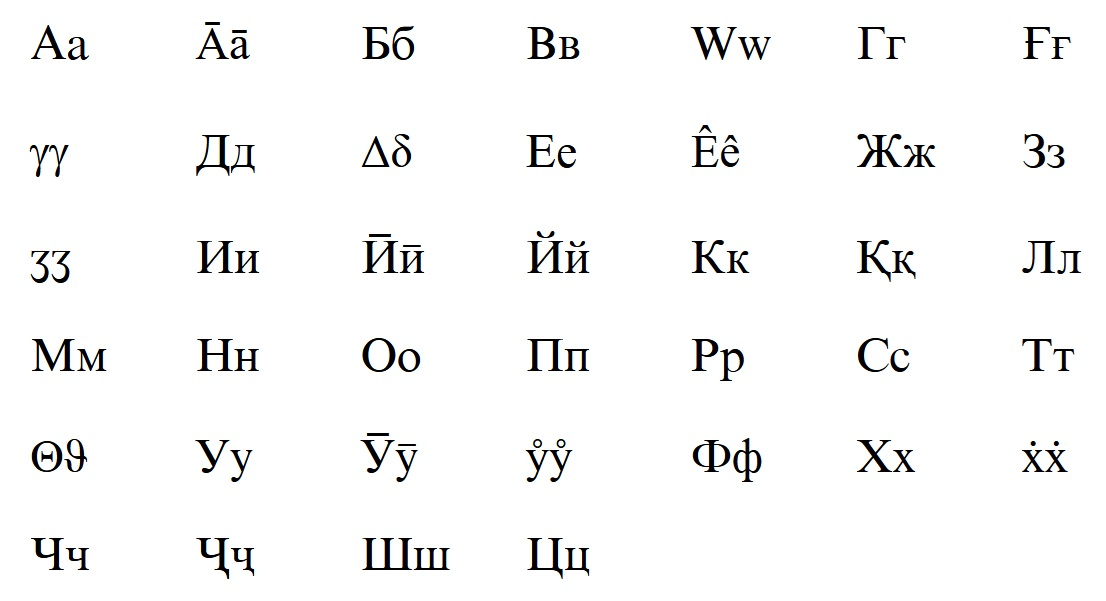
\includegraphics[width=0.8\textwidth]{img/ortho2.jpg}
\end{figure}

\begin{figure}[h]
 \centering
 \caption{Фрагмент публикации \parencite[19]{alinazar2017}}
 \smallskip
 \label{fig:ortho3}
 
\includegraphics[width=0.6\textwidth]{img/ortho3.jpg}
\end{figure}

\pagebreak[4]

Диакритики представляют особую проблему для отображения на~электронных устройствах. Дело в том, что для многих комбинаций букв и диакритик в~Юникоде есть цельный символ. С другой стороны, любые комбинации букв и диакритик можно ввести с помощью композита, то~есть сначала символ буквы, а потом символ диакритики. С точки зрения в~первом случае использован один символ, а~во~втором~— два. Отличие для~рядового пользователя заключается, например, в том, что если на~компьютере набрать цельный символ, а потом нажать клавишу Backspace, то символ удалится целиком; у~композитной буквы же удалится только диакритика. Если возможно, лучше использовать для алфавита цельные символы (об этом подробнее в~\hyperref[ortho-fonts]{Разделе~2.3}).

\subsection{Стандартизированный алфавит} \label{ortho-project}

В этом разделе я представляю свой проект стандартизации шугнанского алфавита, который основан на консенсусном варианте шугнанской кириллицы. Этот вариант наиболее близок к алфавиту, использовавшемуся в последние годы в детских книгах типа \parencite{rizvonshoeva2015} и названному Д.~Эдельман [\cite*[104]{edelman2016}] «наиболее удачным». Он~не~предлагает никаких кардинально новых решений, а наоборот, использует наиболее распространённые практики для передачи шугнанской фонетики на письме. Он является фонематичным и~содержит 39~букв, соответствующих 39~фонемам шугнанского языка. Ниже я перечислю его основные особенности.

Гласная /ɛ/ обозначается символом <Ê~ê>; гласная /ø/ обозначается символом <У̊ у̊>. Долгота гласных обозначается «макроном», то есть горизонтальной чертой сверху. При этом долгота помечается только у~гласных <Ā~ā> /ɑ/, <Ӣ~ӣ> /i/ и <Ӯ~ӯ> /u/ (об этом см.~в~\hyperref[ortho-choice]{Разделе~1.1}). Для~аффрикаты /d͡z/ используется буква «дзе» <Ӡ~ӡ>, заимствованная из~абхазского алфавита. Также используются два очевидных символа из~таджикской кириллицы: <Қ~қ> /q/ и <Ҷ~ҷ> /d͡ʒ/, и латинская буква <W~w>~/w/.

\pagebreak[2]

Межзубные щелевые согласные /ð/ и /θ/ обозначаются греческими буквами «дельта» <Δ~δ> и «тета» <ϴ~θ>. Увулярные щелевые /ʁ/ и /χ/, как~и~в таджикском, обозначаются буквами <Ғ~ғ> и <Х~х>. Для~заднеязычных щелевых /ɣ/ и /x/ используются буквы «латинская гамма» с~гачеком <Ɣ̌~ɣ̌> и «х» с гачеком <Х̌~х̌>\fn{На мой взгляд, наиболее спорным вопросом здесь является необходимость наличия гачека в~букве <Ɣ̌~ɣ̌> /ɣ/. Изначально я считал, что здесь можно обойтись без гачека, так как, в отличие от~<Х̌~х̌>, в предлагаемом алфавите нет соответствующей буквы без гачека, и таким образом, нет~нужды использовать на гамме диакритику. Однако использование диакритики было поддержано сотрудни:цами Института гуманитарных наук г.~Хорог в личной беседе (2023), поэтому я~включаю в~предлагаемый вариант именно гамму с гачеком <Ɣ̌~ɣ̌>.}.

По возможности я использовал цельные символы Юникода (<Ā~ā>, <Ê~ê> и другие). К сожалению, в Юникоде нет цельных символов для~таких букв, как <У̊~у̊>\fn{В Юникоде есть цельный символ <ẙ> (U+1E99), который можно было бы здесь использовать. Однако у этого символа нет заглавного варианта, поэтому он непригоден для полноценного алфавита.}, <Х̌~х̌> и <Ɣ̌~ɣ̌>, поэтому для них использованы композиты, и в некоторых шрифтах их диакритика может «съезжать» в~сторону. Полный проект стандартизации с соответствиями букв и кодов Юникода можно прочитать в~онлайн-документе \parencite{melenchenko2023_unicode} по~ссылке: \i{\href{https://drive.google.com/file/d/1EafEzbr-vX_Y2g6ax41UcUU3RNzY4f0o}{drive.google.com/file/d/1EafEzbr-vX\_Y2g6ax41UcUU3RNzY4f0o}}. Визуально предлагаемый стандартизированный алфавит выглядит так:

\begin{table}[H]
 \centering
 \label{tab:ortho_alphabet}
 \begin{tabular}{cccccccccc}
 Аа & Āā & Бб & Вв & Ww & Гг & Ғғ & Ɣ̌ɣ̌ & Дд & Δδ \\
 Ее & Êê & Жж & Зз & Ӡӡ & Ии & Ӣӣ & Йй & Кк & Ққ \\
 Лл & Мм & Нн & Оо & Пп & Рр & Сс & Тт & Θθ & Уу \\
 Ӯӯ & У̊у̊ & Фф & Хх & Х̌х̌ & Цц & Чч & Ҷҷ & Шш & ~ \\
 \end{tabular}
\end{table}

Для использования этого алфавита на компьютерах я вместе с~Борисом Якубсоном разработал раскладки для Windows и macOS. Расположение букв в этих раскладках основано на стандартной русской схеме ЙЦУКЕН. Некоторые отсутствующие в русском буквы шугнанского алфавита набираются самостоятельными клавишами, другие~— при~помощи вспомогательной клавиши AltGr. Схема раскладок устроена таким образом, чтобы более частотные буквы имели собственные клавиши и располагались ближе к центру для удобства печати\fn{Данные о частотности букв шугнанского алфавита подсчитаны автоматически на материале текста романа Х.~Худобахшова «Зиндаги аз~наw ца~су̊д сар» [\cite*{khudobakhshov2017}].}. Раскладки адаптированы для профессиональной работы с~текстом: кроме букв и~стандартных символов, в них добавлены дополнительные типографские символы (неразрывный пробел, разные виды тире и кавычек и другие знаки пунктуации), схема расположения которых позаимствована из~кириллической раскладки Ильи Бирмана [\cite*{birman}]. Эти раскладки можно скачать на сайте \i{\href{https://shglayouts.pythonanywhere.com}{shglayouts.pythonanywhere.com}}. К~примеру, схема раскладки для Windows выглядит так:

\begin{figure}[H]
 \centering
 \caption{Схема созданной раскладки с шугнанской кириллицей для Windows}
 \smallskip
 \label{fig:ortho4}
 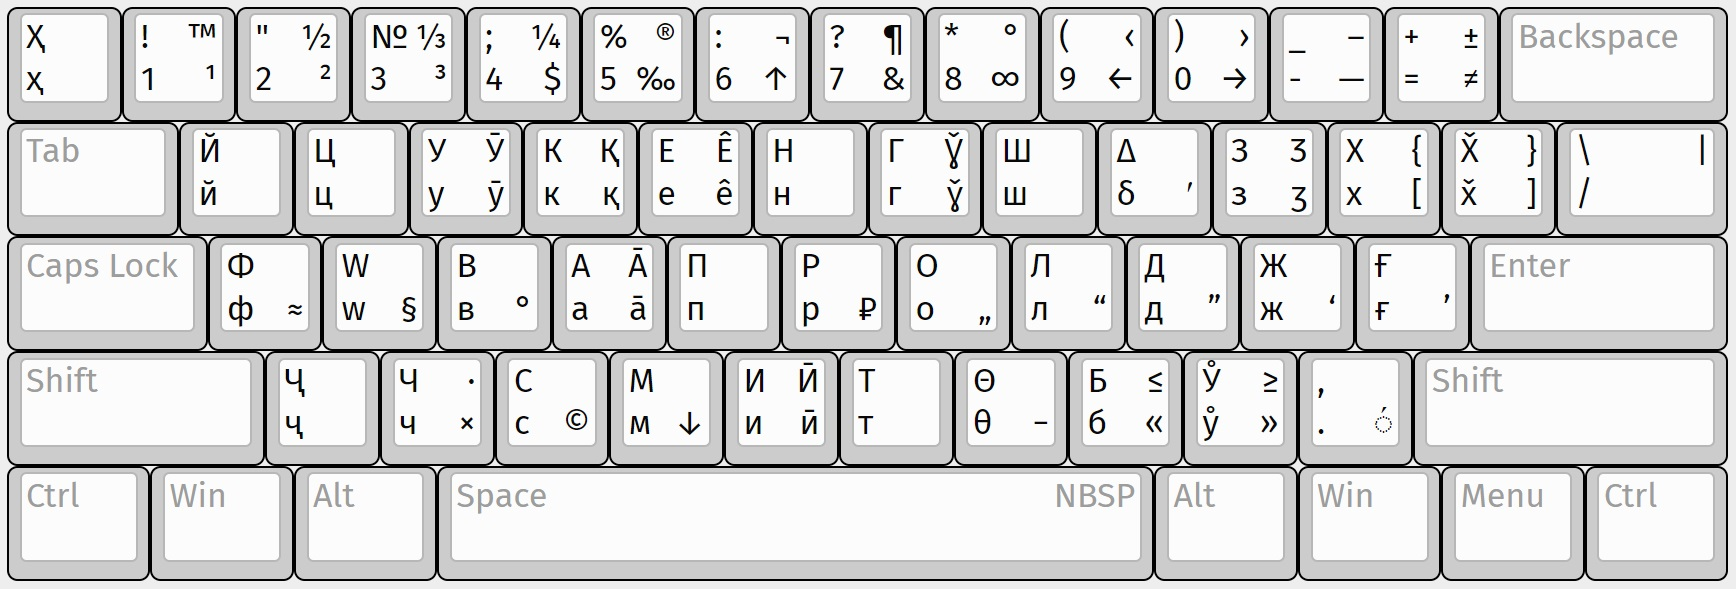
\includegraphics[width=0.8\textwidth]{img/ortho4.jpg}
\end{figure}

Наш проект — далеко не первый опыт создания шугнанской раскладки для компьютеров. К сожалению, в большинстве случаев создаваемые энтузиастами раскладки~не~отличаются удобством и~лёгкостью использования, а кроме того, отражают личные взгляды их~создателей на идеальное устройство шугнанского алфавита, которые только усугубляют проблему разнообразия письменностей. Пример такой раскладки представлен в работе \parencite[21–30]{gulomsafdarov2020}. Во-первых, в~предложенной автором раскладке для обозначения многих согласных используется диакритика «гачек» (<Т̌~т̌> /θ/, <В̌~в̌> /w/ и~другие), что~не~соответствует «консенсусному» алфавиту, представленному выше в~этом разделе. Во-вторых, автор разработал собственную схему расположения шугнанских букв на~клавиатуре вместо того, чтобы модифицировать схемы уже существующих раскладок для~русского или~таджикского. Это означает, что потенциальным пользователям придётся выучить абсолютно новую схему расположения букв, что~кажется мне нецелесообразным. В-третьих, некоторые буквы в~предложенной автором раскладке располагаются на~клавишах для~цифр, а значит, пользователь раскладки лишается возможности использовать цифры. По~этим и другим более мелким причинам я~считаю разработанную нами раскладку более удобной и~рекомендую использовать именно её.

\subsection{Рекомендации по использованию шрифтов} \label{ortho-fonts}

Предложенный выше алфавит и его Юникод-стандарт, на мой взгляд, оптимальны для использования как в быту, так и при профессиональной редактуре текста. При этом в некоторых случаях символы расширенной кириллицы и латиницы, как и диакритики, могут некорректно отображаться на электронных устройствах. Цельные символы Юникода имеют заранее установленное начертание, а начертание композитных букв с~диакритиками зависит от наличия репертуаров. Репертуаром в~Юникоде называется заранее прописанная разработчиками шрифта комбинация буквы и диакритики. Создавая репертуар, разработчики шрифтов указывают, в~каком месте диакритика будет располагаться относительно буквы. Однако разработчики многих шрифтов прописывают репертуары только для самых частых композитов — например, только для композитов с~латинскими буквами. Поэтому при использовании композитов с~кириллическими буквами диакритика может «съезжать» — это связано с~тем, что разработчики не прописали для этой комбинации репертуар, и~тогда диакритика устанавливается в «дефолтном» положении. В~Таблице \ref{tab:ortho3} на~примере буквы <Ê~ê> показано, как отличается отображение цельного символа (слева) и композита (справа) в некоторых известных шрифтах. Можно увидеть, что шрифты Fira Sans и Charis SIL поддерживают кириллические репертуары правильно, а~у~шрифтов Arial и~Times New Roman диакритика «съезжает», если буква записана композитом.

\begin{table}[h]
 \centering
 \caption{Сравнение отображения цельных символов и композитов в~разных шрифтах}
 \smallskip
 \label{tab:ortho3}
 \begin{tabular}{c|cc} \toprule
 шрифт & \makecell{латинская\\«e~с~циркумфлексом»} & \makecell{кириллическая\\«е» + циркумфлекс} \\ \midrule
 {\fontspec{FiraSans-Regular.ttf}Fira Sans} & {\fontspec{FiraSans-Regular.ttf}\large Ê~ê} & {\fontspec{FiraSans-Regular.ttf}\large Е̂~е̂} \\
 {\fontspec{Charis SIL}Charis SIL} & {\fontspec{Charis SIL}\large Ê~ê} & {\fontspec{Charis SIL}\large Е̂~е̂} \\
 {\fontspec{arial.ttf}Arial} & {\fontspec{arial.ttf}\large Ê~ê} & {\fontspec{arial.ttf}\large Е̂~е̂} \\
 {\fontspec{times.ttf}Times New Roman} & {\fontspec{times.ttf}\large Ê~ê} & {\fontspec{times.ttf}\large Е̂~е̂} \\ \bottomrule
 \end{tabular}
\end{table}

\begin{table}[ht]
 \centering
 \caption{Сравнение корректности отображения шугнанских букв с~диакритиками в~разных шрифтах (пример из словарной статьи \i{кур-кур} ‘шорох, шум’ \parencite{karamshoev1991})}
 \smallskip
 \label{tab:ortho4}
 \begin{tabular}{c|l} \toprule
 шрифт & \makecell[l]{пример отображения символов} \\ \midrule
 {\fontspec{arial.ttf}Arial} & \makecell[l]{{\fontspec{arial.ttf}Wāδ пӯрген-ен ас wи ку̊ɣ̌ӡ-ат,} \\ {\fontspec{arial.ttf}~~~каwӣҷ-инд нах̌тойд.}} \\
 {\fontspec{ARIALUNI.ttf}Arial Unicode MS} & \makecell[l]{{\fontspec{ARIALUNI.ttf}Wāδ пӯрген-ен ас wи ку̊ɣ̌ӡ-ат,} \\ {\fontspec{ARIALUNI.ttf}~~~каwӣҷ-инд нах̌тойд.}} \\
 {\fontspec{times.ttf}Times New Roman} & \makecell[l]{{\fontspec{times.ttf}Wāδ пӯрген-ен ас wи ку̊ɣ̌ӡ-ат,} \\ {\fontspec{times.ttf}~~~каwӣҷ-инд нах̌тойд.}} \\
 {\fontspec{Doulos SIL}Doulos SIL} & \makecell[l]{{\fontspec{Doulos SIL}Wāδ пӯрген-ен ас wи ку̊ɣ̌ӡ-ат,} \\ {\fontspec{Doulos SIL}~~~каwӣҷ-инд нах̌тойд.}} \\
 {\fontspec{calibri.ttf}Calibri} & \makecell[l]{{\fontspec{calibri.ttf}Wāδ пӯрген-ен ас wи ку̊ɣ̌ӡ-ат,} \\ {\fontspec{calibri.ttf}~~~каwӣҷ-инд нах̌тойд.}} \\
 {\fontspec{cambria.ttc}Cambria} & \makecell[l]{{\fontspec{cambria.ttc}Wāδ пӯрген-ен ас wи ку̊ɣ̌ӡ-ат,} \\ {\fontspec{cambria.ttc}~~~каwӣҷ-инд нах̌тойд.}} \\
 {\fontspec{CharisSIL-Regular.ttf}Charis SIL} & \makecell[l]{{\fontspec{CharisSIL-Regular.ttf}Wāδ пӯрген-ен ас wи ку̊ɣ̌ӡ-ат,} \\ {\fontspec{CharisSIL-Regular.ttf}~~~каwӣҷ-инд нах̌тойд.}} \\
 {\fontspec{FiraSans-Regular.ttf}Fira Sans} & \makecell[l]{{\fontspec{FiraSans-Regular.ttf}Wāδ пӯрген-ен ас wи ку̊ɣ̌ӡ-ат,} \\ {\fontspec{FiraSans-Regular.ttf}~~~каwӣҷ-инд нах̌тойд.}} \\
 {\fontspec{GentiumBookPlus-Regular.ttf}Gentium Book Plus} & \makecell[l]{{\fontspec{GentiumBookPlus-Regular.ttf}Wāδ пӯрген-ен ас wи ку̊ɣ̌ӡ-ат,} \\  {\fontspec{GentiumBookPlus-Regular.ttf}~~~каwӣҷ-инд нах̌тойд.}} \\
 {\fontspec{helvetica_regular.otf}Helvetica} & \makecell[l]{{\fontspec{helvetica_regular.otf}Wāδ пӯрген-ен ас wи ку̊ɣ̌ӡ-ат,} \\ {\fontspec{helvetica_regular.otf}~~~каwӣҷ-инд нах̌тойд.}} \\
 {\fontspec{Noto Sans}Noto Sans} & \makecell[l]{{\fontspec{Noto Sans}Wāδ пӯрген-ен ас wи ку̊ɣ̌ӡ-ат,} \\ {\fontspec{Noto Sans}~~~каwӣҷ-инд нах̌тойд.}} \\ 
 Noto Serif & \makecell[l]{Wāδ пӯрген-ен ас wи ку̊ɣ̌ӡ-ат, \\ ~~~каwӣҷ-инд нах̌тойд.} \\
 {\fontspec{Roboto-Regular.ttf}Roboto} & \makecell[l]{{\fontspec{Roboto-Regular.ttf}Wāδ пӯрген-ен ас wи ку̊ɣ̌ӡ-ат,} \\  {\fontspec{Roboto-Regular.ttf}~~~каwӣҷ-инд нах̌тойд.}} \\
 {\fontspec{Trebuchet MS}Trebuchet MS} & \makecell[l]{{\fontspec{Trebuchet MS}Wāδ пӯрген-ен ас wи ку̊ɣ̌ӡ-ат,} \\ {\fontspec{Trebuchet MS}~~~каwӣҷ-инд нах̌тойд.}} \\ \bottomrule
 \end{tabular}
\end{table}

Это одна из причин, по которой предпочтительно использовать цельные символы. К примеру, буква <Ê~ê> в стандартизированном алфавите, который я предложил в \hyperref[ortho-project]{Разделе~2.2}, кодируется цельным символом, и поэтому диакритика не съезжает. Однако, к сожалению, не~для~всех предложенных букв с диакритиками в Юникоде есть цельные символы. Буквы <У̊~у̊>, <Х̌~х̌> и <Ɣ̌~ɣ̌> нельзя записать цельно, поэтому для~них мы используем композиты, а они могут некорректно отображаться в некоторых шрифтах. Как можно увидеть в~Таблице \ref{tab:ortho4} ниже, в шрифтах Arial и Times New Roman диакритика расположена некорректно у двух букв: <У̊~у̊> и <Х̌~х̌>. В некоторых шрифтах встречается и~более серьёзная проблема: в шрифте нет даже самого начертания определённых символов, и в современных программах такие символы автоматически отображаются с помощью другого шрифта. К примеру, как~показано в~Таблице \ref{tab:ortho4}, в~шрифте Trebuchet MS нет многих символов шугнанской кириллицы.

Проблема некорректного отображения решается использованием шрифтов, которые поддерживают шугнанские символы. Шрифты Arial Unicode MS, Calibri, Cambria, входящие в стандартный пакет Windows, правильно отображают буквы шугнанской кириллицы. Кроме того, есть ряд подходящих шрифтов, которые распространяются по свободной лицензии (их можно найти и бесплатно скачать в интернете): это Andika, Charis SIL, DejaVu Sans, DejaVu Serif, Doulos SIL, Fira Sans, Gentium Plus, New CM Sans, New CM Serif и Noto Sans.

Для~многих популярных шрифтов, неправильно отображающих шугнанские символы, можно найти более подходящие аналоги. Так,~вместо Times New Roman можно пользоваться бесплатным шрифтом Doulos SIL, который визуально похож на~Times New Roman. Вместо стандартного Arial можно пользоваться его расширенной версией Arial Unicode MS (см.~Таблицу \ref{tab:ortho4}).

\begin{figure}[ht]
 \centering 
 \caption{Сравнение отображения таджикского текста из учебника Аламшоева [\cite*[4]{alamshoev2014}] в~«таджикском» шрифте Times New Roman Tj и обычном Times New Roman}
 \smallskip
 \label{fig:ortho5}

 \begin{quote} \begin{spacing}{1.2}
 \b{Times New Roman Tj}: {\fontspec{Times_New_Roman_Tj.ttf}Ин дастур, ки ба курси шунавандагони забони шуѓнонї, яке аз ќадимтарин забонњои эронї бахшида шудааст, барои хубтар аз худ кардани ин забон пешбинї шудааст. Дастур асосан барои хонандагони тољикзабон, ки мехоњанд забони шуѓнониро аз худ кунанд, тартиб дода шудааст. Пеш аз њама муаллим бояд ба шунавандагон дар бораи  таърихи пайдоиши забонњои эронї ва алалхусус, гурўњи шарќии он — забонњои помирї маълумот дињад.}
 \end{spacing} \end{quote}

 \begin{quote} \begin{spacing}{1.2}
 \b{Times New Roman}: {\fontspec{times.ttf}Ин дастур, ки ба курси шунавандагони забони шуѓнонї, яке аз ќадимтарин забонњои эронї бахшида шудааст, барои хубтар аз худ кардани ин забон пешбинї шудааст. Дастур асосан барои хонандагони тољикзабон, ки мехоњанд забони шуѓнониро аз худ кунанд, тартиб дода шудааст. Пеш аз њама муаллим бояд ба шунавандагон дар бораи  таърихи пайдоиши забонњои эронї ва алалхусус, гурўњи шарќии он — забонњои помирї маълумот дињад.}
 \end{spacing} \end{quote}
\end{figure}

\pagebreak[3]

Наконец, стоит обратиться к такому явлению, как «таджикские шрифты». Это модифицированные версии известных шрифтов, в~которых вместо дополнительных символов таджикской кириллицы используются другие символы, но они отображаются как~таджикские буквы (см.~Рисунок~\ref{fig:ortho5}). Например, буква, которая в одном из самых употребительных «таджикских шрифтов» Times New Roman Tj выглядит как <Ҳ~ҳ>, на самом деле кодируется символом для буквы из~сербского алфавита <Њ~њ>. По-видимому, создание таких кустарных инструментов для работы с текстом приходится на 1990-е годов, когда~распространённые компьютерные шрифты не~поддерживали буквы таджикского алфавита \parencite{graschenko2011}. В~настоящее время буквы как~таджикского, так~и~шугнанского алфавитов поддерживаются огромным количеством шрифтов, и~необходимости в~«таджикских шрифтах»-обманках нет. Однако они всё ещё активно используются в работе как с таджикским, так~и с~шугнанским языком. К~примеру, учебник Аламшоева [\cite*{alamshoev2014}], по-видимому, был напечатан с~помощью Times New Roman Tj.

Я не рекомендую использовать «таджикские шрифты» для~работы с~шугнанскими (как и с таджикскими) текстами. Набранный таким образом текст будет корректно отображаться только в Microsoft Word (или~аналогичных редакторах), но~при копировании текста в~другие программы, где~выбор «таджикских шрифтов» недоступен (например, в~веб-браузер) или~при~открытии на~устройстве, где не установлен нужный шрифт, он~станет нечитаемым (см.~Рисунок~\ref{fig:ortho5}).

С~помощью инструментов, представленных в статье (в частности, с~помощью раскладок для~компьютеров и~рекомендованных шрифтов), любой пользователь компьютеров на~Windows или macOS сможет быстро и~удобно печатать аккуратно выглядящие тексты на~шугнанском языке, не~прибегая к~самостоятельному поиску символов,~«таджикским шрифтам» или~другим сложным техническим находкам.

%%% ЛЕКСИЧЕСКАЯ ТИПОЛОГИЯ
\chapter*{Система глаголов движения вниз в~шугнанском языке}
\addcontentsline{toc}{chapter}{\textit{Е.~Рахилина, Ш.~Некушоева}. \textbf{Система глаголов движения вниз в~шугнанском языке}}
\setcounter{section}{0}
\chaptermark{Система глаголов движения вниз в~шугнанском языке}
\label{chapter-rakh-down}

\begin{customauthorname}
Екатерина Рахилина, Шахло Некушоева
\end{customauthorname}

\begin{englishtitle}
\i{Falling verbs in Shughni\\{\small Ekaterina Rakhilina, Shahlo Nekushoeva}}
\end{englishtitle}

\begin{abstract}
Статья описывает систему глаголов падения в одном из памирских языков (восточно-иранских) — шугнанском. Она опирается как на первичные данные, специально собранные для этой статьи, так и на данные словаря Д.~Карамшоева [\cite*{karamshoev1988}], проверенные во время полевых исследований. Показано, что в шугнанском действует доминантный глагол \i{wêх̌тоw}, который в целом покрывает основные ситуации падения. Параллельно в этом языке имеется несколько «малых» глаголов, для описания резкого обрушения (\i{чук δêдоw}), особой траектории падения (фразовый глагол \i{оле ситтоw} ‘падать кубарем’) и нарушения целостности (\i{нихих̌тоw} ‘разваливаться’). В качестве глаголов падения в шугнанском функционируют и глаголы других, семантически близких, полей — поля вращения (\i{гāх̌тоw} ‘поворачиваться’), поля прыгания (\i{зибидоw} ‘прыгать’) и поля удара (\i{δêдоw} ‘падать, ударяться’). Типологически материал шугнанского ценен тем, что позволяет выявить прототипические фреймы, обеспечивающие семантическое пересечение выделенных глаголов с полем падения. Для вращения это падающие деревья, для прыгания — открепление функционально связанных друг с другом объектов и частей от целых, для удара — падение с акцентом на результат (в первую очередь, падение человека с указанием части тела, приходящей в контакт с твёрдой поверхностью).
\end{abstract}

\begin{keywords}
лексическая типология, метафора, метонимия, падение, памирские языки, топология предметов, шугнанский язык.
\end{keywords}

\vfill

\begin{eng-abstract}
The article deals with the system of falling verbs in Shughni, which is one of the Pamir languages of the Southeastern Iranian group. It presents the original data collected from native speakers and the data from Karamshoev’s dictionary [\cite*{karamshoev1988}], checked during our field work.

The paper argues that the Shughni system of falling verbs, though not dominant in the proper sense of the term, has a central specialized verb \i{wêx̌tow} covering the main situations of falling: falling from an elevated surface (a cup from the table), falling of a person, falling of a vertically oriented artifacts like road poles, etc.

There are also several “minor” verbs of falling: for falling with non-vertical trajectory (etymologically opaque phrasal verb \i{ole sittow}), for collapsing (\i{čuk δêdow}) or falling accompanied with disintegration, like falling into pieces / fragments or falling of a pipe / heap of objects (\i{nixix̌tow}). In addition, there are non-falling verbs which are used for lexification of some important falling frames. For example, the verb of rotation \i{gāx̌tow} with the meaning ‘turn’ is used for trees falling because of the strong wind; the verb of upward motion \i{zibidow} ‘jump’ is used to denote different situations of detachment of one object from another including parts from wholes, like a damaged wheel being detached from the car during the trip. The causative verb of destruction \i{δêdow} ‘hit’ (which by default denotes aggressive physical effect of one person to another), when applied to falling situations, means falling of an object from above with the clear accent on the result.

The Shughni system reveals the main oppositions relevant for falling verbs cross-linguistically. However, this system is quite abnormal, because apart from the central verb \i{wêx̌tow} it does not have dedicated verbs of falling (with some very marginal exceptions): all the other markers are borrowed from other semantic fields. It means that Shughni data may serve as an important source for lexical typology illuminating the points of intersection of {\sc falling} with other semantic domains.
\end{eng-abstract}

\begin{eng-keywords}
lexical typology, metaphor, metonymy, falling, Pamir languages, topological features, Shughni.
\end{eng-keywords}

\begin{initialprint}
\fullcite{rakhilina_nekushoeva2020}\end{initialprint}

\section{Введение} \label{down-intro}

Шугнанский язык является одним из самых крупных памирских языков. Он относится к восточно-иранской группе иранских языков. Шугнанцы (численностью около 90~тысяч) живут в основном в Горно-Бадахшанской автономной области Таджикистана (административный центр — город Хорог, примерно в пятистах километрах от Душанбе, у слияния рек Пяндж и Гунд), в Шугнанском и Рошткалинском районах. Есть шугнанцы и в Бадахшанской провинции Афганистана, на другой стороне Пянджа, но наши данные собраны на территории Таджикистана.

Основные описания шугнанского изданы во второй половине прошлого века. Это, прежде всего, небольшое собрание текстов со словарем \parencite{zarubin1960}, а также замечательный словарь \parencite{karamshoev1988}, который во многом служил для нас точкой отсчёта.

Из грамматических особенностей шугнанского, важных при чтении нашей статьи, отметим, что в шугнанском (как и в других индо-иранских языках) предикатные значения в основном выражаются так называемыми сложными глаголами. Однако поскольку статья касается самой базовой лексики, здесь нам в основном встретятся как раз простые глаголы. Им свойственна нетривиальная глагольная морфология, характерная для шугнанского, и прежде всего, многоосновность. Сложные для анализа фрагменты мы старались снабжать необходимыми морфологическими комментариями помимо глосс.

История нашего описания падения в шугнанском довольно парадоксальна — и в определенном отношении показательна. Дело в том, что языковой материал собирался в два этапа: сначала в Москве с квалифицированным носителем, а затем в условиях совместной Памирской экспедиции Школы лингвистики НИУ~ВШЭ и Института памирских языков. При этом наши первоначальные, московские данные свидетельствовали о том, что в шугнанском действует доминантная система глаголов падения. Другими словами, эти данные говорили о том, что там есть очень общий (то есть доминирующий) глагол \i{wêх̌тоw} (с основой настоящего времени \i{wох̌}- и формой прошедшего времени \i{wêх̌т}), который соотносится с самыми разными типами падения, покрывая и падение человека, и камня в реку, и моста, провалившегося под тяжестью машины, и веревки, соскочившей с гвоздя, и выпавших зубов, и прочее.

Интересно то, что все полученные в ходе этой работы примеры при последующей проверке экспертами полностью подтвердились — однако их интерпретация изменилась: со сбором новых данных, наше исходное представление о шугнанской системе падения подверглось существенной коррекции. Обнаружилось, что на самом деле в зоне падения в шугнанском языке действует дистрибутивная, а не доминантная система, со сложным распределением всего пространства поля между как минимум шестью предикатами, специфику паденческого значения каждого из которых мы будем подробно обсуждать в этой статье, а именно: \i{wêх̌тоw}, \i{гāх̌тоw}, \i{нихих̌тоw}, \i{зибидоw}, \i{δêдоw}, а также фразеологизованной конструкцией \i{оле ситтоw} — если не считать глаголов движения жидкости, которые мы здесь рассмотреть не сможем ввиду объемности имеющегося материала\fn{Заметим, что все это глаголы моментальные, практически всегда они употребляются в перфективных контекстах, соответственно, в формах прошедшего времени: \i{wêх̌т}, \i{гāх̌т}, \i{нихух̌т} [{\sc m.sg}] / \i{нихах̌т} [{\sc f/pl}], \i{зибуд} [{\sc m.sg}] / \i{зибад} [{\sc f/pl}], \i{δод}, \i{оле сут} [{\sc m.sg}] / \i{оле сат} [{\sc f/pl}].}.

В этой системе работают следующие типологически релевантные противопоставления, которые мы подробно рассмотрим в соответствующих разделах статьи:

\begin{itemize}
  \item по топологии падающего объекта (\hyperref[down-topology]{Раздел~2})
  \item по топологии (траектории) самого падения, включая так называемое «рефлексивное» падение (\hyperref[down-geometry]{Раздел~3})
  \item по значимости начальной / конечной точки (\hyperref[down-endpoint]{Раздел~4})
\end{itemize}

В \hyperref[down-conclusion]{Разделе~5} мы подведем итоги анализа этого материала.

\section{Топология падающего субъекта: \i{wêх̌тоw} и~\i{гāх̌тоw}} \label{down-topology}

Как обычно, по этому геометрическому параметру противопоставлены два типа ситуаций: падение с приподнятой поверхности, для которого не важна форма и ориентация объекта (см.~\hyperref[down-wextow]{Раздел~2.1}), и падение жёсткого вертикально ориентированного объекта, в результате которого этот объект оказывается на той же плоскости, но в горизонтальном положении (см.~\hyperref[down-vertical]{Раздел~2.2}).

\subsection{\i{Wêх̌тоw}: падение сверху, сопутствующие значения и метафорика} \label{down-wextow}

Падение с приподнятой поверхности обозначается частотным шугнанским глаголом \i{wêх̌тоw}, который сочетается с предлогом \i{аз} с широким аблативным значением ‘с / из / сверху’\fn{В основном наши примеры собраны во время полевой работы; в словарных примерах указывается источник.}:

\ex<exdown1>
\begingl
\gla Қалам аз му сӯмка=нд \b{wêх̌-т}.//
\glc карандаш {\sc el} {\sc pron.1sg.o} сумка={\sc loc} падать-{\sc pst}//
\glft ‘Из моей сумки \b{выпал} карандаш.’//
\endgl \xe

\ex<exdown2>
\begingl
\gla Жиниҷ аз дишӣд=ти \b{wêх̌-т}.//
\glc снег {\sc el} крыша={\sc sup} падать-{\sc pst}//
\glft ‘Снег \b{упал} с крыши.’//
\endgl \xe

\ex<exdown3>
\begingl
\gla Жӣр аз тӣр=ти \b{wêх̌-т}.//
\glc камень {\sc el} верх={\sc sup} падать-{\sc pst}//
\glft ‘Сверху \b{упал} камень.’//
\endgl \xe

\ex<exdown4>
\begingl
\gla Wиδич-буц аз ху рêӡ=анд \b{wêх̌-т}.//
\glc птица-детёныш.{\sc m} {\sc el} {\sc refl} гнездо={\sc loc} падать-{\sc pst}//
\glft ‘Птенец \b{выпал} из своего гнезда.’//
\endgl \xe

\ex<exdown5>
\begingl
\gla Йу кӯдак аз стӯл=ти \b{wêх̌-т}.//
\glc {\sc d3.m.sg} ребёнок {\sc el} стул={\sc sup} падать-{\sc pst}//
\glft ‘Ребёнок \b{упал} со стула.’//
\endgl \xe

Как мы уже говорили, помимо падения с поверхности, этим глаголом может описываться падение человека (\gethref{exdown6}), но также и обвал ветхого моста, падение самолёта, птицы из гнезда, ключа из кармана, человека с балкона, машины, мяча, шляпы, верёвки, соскочившей с гвоздика, и многое другое (подробнее см.~в следующих разделах).

\ex<exdown6>
\begingl
\gla Ɣ̌иник ху поδ=и пи жӣр=анд ~~~~~~~~~~~~~~~~~~~~~~~~~~~~~~~~~~~~~ ҷук-т=ху \b{wêх̌-т}.//
\glc женщина {\sc refl} нога={\sc 3sg} {\sc up} камень={\sc loc} ~ удариться-{\sc pst=and1} падать-{\sc pst}//
\glft ‘Женщина \b{споткнулась} о камень и упала.’//
\endgl \xe

Глагол \i{wêх̌тоw}, по \parencite[360–361]{karamshoev1988}, имеет довольно широкий круг метафорических значений. Часть из них может быть описана как обычная метафора, то есть переход из семантической зоны физического движения к абстрактному, ср.~‘лишиться должности’ (\gethref{exdown8}) или ‘выпасть’ как ‘родиться’ (\gethref{exdown9})\fn{Для примеров со значением ‘родиться’ возможна и другая трактовка: не исключено, что глагол \i{wêх̌тоw} в таких случаях используется в качестве табу. Например, кто-то из домочадцев входит в дом с известием о рождении телёнка, но для того чтобы потусторонние силы не услышали и не навредили только что родившемуся телёнку, используется глагол \i{wêх̌тоw}, как если бы телёнок упал и умер.}:

\ex<exdown7>
\begingl
\gla Бало аз осму̊н ца \b{wох̌т}, ~~~~~~~~~~~~~~~~~~~~~~~~~~~~~~~~~~~~~~~~~~~~~~~~~~~~~~~~~~~~ бардохт чӣд-оw даркор.//
\glc беда {\sc el} небо {\sc subd} падать.{\sc prs.3sg} ~ терпение делать.{\sc inf-purp} нужно//
\glft ‘Если \b{случится} беда, нужно смириться.’//
\endgl \xe

\ex<exdown8>
\begingl
\gla Йу аз ху амал \b{wêх̌-т}.//
\glc {\sc d3.m.sg} {\sc el} {\sc refl} должность падать-{\sc pst}//
\glft ‘Он лишился (буквально ‘\b{выпал} из’) своего чина.’ \trailingcitation{\parencite[84]{karamshoev1988}}//
\endgl \xe

\ex<exdown9>
\begingl
\gla Шӣг-буц бехилӣwанд-аθ аз ху нāн \b{wêх̌-т}.//
\glc телёнок-детёныш.{\sc m} неожиданный-{\sc adv} {\sc el} {\sc refl} мама падать-{\sc pst}//
\glft ‘Телёнок \b{родился} сразу.’//
\endgl \xe

Другие можно рассматривать как результат частичной грамматикализации, то есть превращения \i{wêх̌тоw} в лёгкий глагол со значением ‘попадать в ситуацию Р / оказываться в Р’, вызванного идеей спонтанности и неконтролируемости, свойственной падению:

\ex<exdown10>
\begingl
\gla Дис гандā wазийат=анд=ум \b{wêх̌-т}.//
\glc такой плохой положение={\sc loc=1sg} падать-{\sc pst}//
\glft ‘Я \b{попал} в тяжёлое положение.’//
\endgl \xe

Эти сдвиги глаголов с семантикой падения широко распространены в языках мира\fn{См. другие статьи в специальном выпуске журнала \i{Acta Linguistica Petropolitana}, в котором была напечатана эта статья: \parencite{rakhilina_etal2020}~— \i{прим.~переиздания}.}. Вместе с тем шугнанский даёт любопытные дополнения к общему стандарту. Действительно, как и в других языках, шугнанское \i{wêх̌тоw}, имеющее довольно общую семантику, используется для выражения потери функциональности, ср. аналогичные шугнанским русские примеры типа \i{трон пал} / \i{власть пала} (= ‘перестала функционировать’). Особенность шугнанского в том, что идея потери функциональности конкретных артефактов (а не только абстрактных сущностей), по крайней мере в некоторых фразеологизмах (возможно, отражающих некоторое предшествующее состояние его лексической системы) тоже может выражаться через апелляцию к идее падения. Ср.~\parencites[531]{karamshoev1991}[360]{karamshoev1988}.

\ex<exdown11>
\begingl
\gla Му рӯшт куртā \b{wêх̌-ч}, ā йу сāвӡ ~~~~~~~~~~~~~ ғал наw-аθ.//
\glc {\sc pron.1sg.o} красный платье падать-{\sc pf} а {\sc d3.m.sg} зеленый ~ ещё новый-{\sc adv}//
\glft ‘Моё красное платье \b{износилось}, а то зелёное ещё совсем новое.’//
\endgl \xe

\ex<exdown12>
\begingl
\gla Йу̊д-ирд ачаθ сандāл нист, фук=аθ=ен \b{wêх̌-ч}.//
\glc {\sc d1-dat} совсем старая\_обувь быть.{\sc neg} все={\sc int=3pl} падать-{\sc pf}//
\glft ‘Здесь нет даже никаких потрёпанных сапог, все \b{порвались}.’//
\endgl \xe

Пример (\gethref{exdown13}) представляет контекст другого рода, где \i{wêх̌тоw} применён к части тела и имеет уникальное значение ‘мёрзнуть, стыть’ с неясной историей, однако он тоже может быть проинтерпретирован как выражение потери функциональности:

\ex<exdown13>
\begingl
\gla Тар дарго дис шито, му δуст-ен=ен тар \b{wêх̌-т}.//
\glc {\sc eq} двор такой холодный {\sc pron.1sg.o} рука-{\sc pl=3pl} {\sc eq} падать-{\sc pst}//
\glft ‘На улице так холодно, мои руки замёрзли (=~букв. мои руки \b{упали})’//
\endgl \xe

\subsubsection*{Примечание}

В связи с только что сказанным обратим внимание на любопытную фразему \i{wêх̌ч-питêwҷ одам}, не отмеченную у Карамшоева: так говорят о неуклюжем, никчёмном человеке. По структуре это конструкция повтора — два глагола близкой семантики идут подряд в одной и той же форме: \i{wêх̌ч} — перфектная форма глагола \i{wêх̌тоw} ‘падать’, а \i{питêwҷ} — перфект от \i{питêwдоw} — ‘бросать, кидать’.

Карамшоев приводит примеры такой последовательности, но в глагольном контексте, где она приобретает значение ‘заброшенный, брошенный’: \i{йу wêх̌ч-питêwҷ ред} — он остался без присмотра (то есть ‘брошенный, безнадзорный, оставленный всеми’ \parencite[335]{karamshoev1988}). См.~там же в значении ‘брошенный’:

\ex<exdown14>
\begingl
\gla Wам пуц [\b{wêх̌-ч} \b{питêw-ҷ}] вуд=ат, ~~~~~~~~~~~~ шич ғулā сут.//
\glc {\sc d3.f.sg.o} сын падать-{\sc pf} бросать-{\sc pf} быть.{\sc pst.m.sg=and2} ~ сейчас большой стать.{\sc pst.m.sg}//
\glft ‘Её сын был \b{безнадзорным}, да вырос теперь.’ \trailingcitation{\parencite[335]{karamshoev1988}}//
\endgl \xe

Значения ‘никчёмный / неуклюжий’ данная фразема в глагольных контекстах не имеет, но, по-видимому, приобретает его в именных — и не исключено, что в этом случае такой метафорический эффект тоже связан с идеей потери функциональности.

\ex<exdown14b>
\begingl
\gla Йи [\b{wêх̌-ч} \b{питêw-ҷ}] одам йу вуд.//
\glc {\sc indef} падать-{\sc pf} бросать-{\sc pf} человек {\sc d3.m.sg} быть.{\sc pst.m.sg}//
\glft ‘Он был таким \b{неуклюжим} человеком.’//
\endgl \xe

Именно широкая сочетаемость \i{wêх̌тоw} и создает иллюзию существования на его основе доминантной системы. Однако, как мы увидим дальше, в шугнанском есть и другие возможности выразить идею падения.

\subsection{Падение вертикальных объектов} \label{down-vertical}

Одна из таких возможностей связана с ситуацией падения вертикального вытянутого предмета, которую в шугнанском часто выражает глагол \i{гāх̌тоw}. Именно он и только он применяется для описания деревьев, вывернутых из земли сильным ветром, или столбов — при похожих обстоятельствах. Применительно к этим ситуациям \i{wêх̌тоw} малоприемлем:

\ex<exdown15>
\begingl
\gla Хах̌ х̌ӯӡ сут=ху, йā дирахт ~~~~~~~~~~~~~~~~ \b{гāх̌-т} / *wêх̌-т.//
\glc твёрдый ветер стать.{\sc pst.m.sg=and1} {\sc d3.f.sg} дерево ~ повернуться-{\sc pst} ~~~~~~ падать-{\sc pst}//
\glft ‘От сильного ветра то дерево \b{упало}.’//
\endgl \xe

В случае срубленных / сломанных деревьев / столбов возможна вариативность в ответах носителей языка, связанная с архаизацией глагола \i{гāх̌тоw}. Старшее поколение для описания падения дерева обязательно использует глагол \i{гāх̌тоw}, однако молодое поколение употребляет глагол \i{wêх̌тоw}. При этом соответствующая каузативная ситуация выражается глаголом \i{гарδентоw}, производным именно от \i{гāх̌тоw}:

\ex<exdown16>
\begingl
\gla Столба ар пу̊нд \b{wêх̌-т} / \b{гāх̌-т}.//
\glc столб {\sc down} дорога падать-{\sc pst} ~~~~~~ повернуться-{\sc pst}//
\glft ‘Столб \b{упал} на дорогу.’//
\endgl \xe

\ex<exdown17>
\begingl
\gla Wуз=ум дам дарахт тавāр қати \b{гарδ-ен-т}.//
\glc {\sc pron.1sg=1sg} {\sc d2.f.sg.o} дерево топор {\sc com} повернуться-{\sc caus-pst}//
\glft ‘Я \b{срубил} это дерево.’//
\endgl \xe

Заметим, что сам класс прототипически вертикальных объектов, которые выделяются особой глагольной лексемой в ситуации падения, в шугнанском не совсем обычен. В частности, падение людей описывается не этим выделенным глаголом, а исключительно общим глаголом \i{wêх̌тоw}, см.~выше пример (\gethref{exdown6})\fn{К ситуации падения других вертикальных природных объектов, таких как цветы или высокая трава, \i{гāх̌тоw} тоже не применяется — чего, впрочем, вполне можно ожидать: топология их падения несколько другая: это нежёсткие объекты, хотя и вертикальные.}. Это удивительно, потому что было бы естественно полагать, что соответствующий топологический тип объектов формируется как антропоцентричный, и все предметы, которые в него попадают (как деревья или столбы), лишь уподобляются человеческим существам. Шугнанский материал показывает, что это предположение далеко не всегда верно.

Падение крупных артефактов, имеющих вертикальную ориентацию (ср.~‘дом’ или ‘шкаф’), допускает вариативность в выборе глагола, но здесь некоторые эксперты разрешают глагол \i{гāх̌тоw}\fn{О других лексических маркерах падения для дома / стены и подобных объектов — см.~ниже.}.

\ex<exdown18>
\begingl
\gla Хах̌ заминҷунби сут=ху, ~~~~~~~~~~~~~~~~~~~~~~~~~~~~~~~~~~~~~~~~~ мāш чӣд \b{гāх̌-т}.//
\glc твёрдый землетрясение стать.{\sc pst.m.sg=and1} ~ {\sc pron.1pl} дом повернуться-{\sc pst}//
\glft ‘Наш дом \b{рухнул} от сильного землетрясения.’//
\endgl \xe

Ещё один характерный для \i{гāх̌тоw} тип употреблений в зоне падения артефактов — это вертикальные контейнеры с содержимым, как например, ведро с водой, см.~пример (\gethref{exdown19})\fn{Ср.~другой вариант того же предложения с глаголом \i{тис ситтоw} ‘сыпаться, литься’: \i{йā х̌ац чалак қати \b{тис сат}} [{\sc d3.f.sg} вода ведро {\sc com} разлитый стать.{\sc pst.f/pl}]. Контекст опрокинутого сосуда достаточно частотный, а варианты с \i{тис ситтоw} и \i{гāх̌тоw} практически синонимичны: фактически глагол \i{гāх̌тоw} в этих контекстах импликативно получает семантику ‘проливаться’. Именно поэтому в \parencite{karamshoev1988} для него отмечается и это значение тоже, хотя строго говоря, это не так.}. Заметим, что и в русском этот тип артефактов лексически выделен: в частности, к ним применяется особый предикат \i{опрокинуться}, совмещающий этот тип падения только с падением людей навзничь.

\ex<exdown19>
\begingl
\gla Х̌ац \b{гāх̌-т} чалак қати.//
\glc вода повернуться-{\sc pst} ведро {\sc com}//
\glft ‘Ведро с водой \b{опрокинулось}.’ \trailingcitation{\parencite[387]{karamshoev1988}}//
\endgl \xe

В отличие от русского, где пустой контейнер может в отношении глаголов падения вести себя точно так же, как и полный, в шугнанском падение пустого контейнера описывается исключительно общим глаголом \i{wêх̌тоw}. Точно так же падение человека навзничь (например, сидящего на стуле), которое в русском объединено с контейнерами, глагол \i{гāх̌тоw} тоже не покрывает: человек вообще исключён из зоны действия \i{гāх̌тоw}.

\pagebreak[4]

Однако падение самого стула назад, на спинку, выражается именно с помощью \i{гāх̌тоw} — а глагол \i{wêх̌тоw}, как мы и ожидаем, соответствует его падению в любую другую сторону. Формально такое распределение вполне мотивировано: ведь только со спинкой стул нам «виден» как вертикальный объект, но в целом избирательность сочетаемости \i{гāх̌тоw} удивляет. Однако объяснение такому распределению легко найти, если учесть, что по своему исходному значению \i{гāх̌тоw} — это \b{доминантный глагол вращения объекта} \parencite[387]{karamshoev1988}, который применим к вращению и вокруг своей, и вокруг внешней оси, и в том числе, по свидетельству автора словаря, описывает множественные обороты. Правда, в качестве подтверждения последнему, Карамшоев приводит только один пример:

\ex<exdown20>
\begingl
\gla Лāк йид хидорҷ жӣр \b{гāрδд}=ат, ~~~~~~~~~~~~~~ wуз=та ди хидорҷ илат wизу̊н-ум.//
\glc пусть {\sc d2.sg} мельница камень повернуться.{\sc prs.3sg=and2} ~~~~~~~~~~~~~~ {\sc pron.1sg=fut} {\sc d2.m.sg.o} мельница секрет знать-{\sc prs.1sg}//
\glft ‘Пусть жернов мельницы \b{вращается}, и я определю дефект мельницы.’//
\endgl \xe

Носители современного шугнанского такого рода употребления не признают: они считают, что у \i{гāх̌тоw} есть только значение одиночного неполного оборота, поворота в сторону или переворота, ср.~также более идиоматичные конструкции: ‘подвернул ногу’, ‘переправился на другую сторону реки’ и другие подобные\fn{Возможно, это исходно отымённый глагол, восходящий к семантике круга, ср.~\i{гарδā} ‘лепёшка’ (только круглая), \i{гарδов} ‘водоворот’.}:

\ex<exdown21>
\begingl
\gla Йā дивӯск пāли \b{гāх̌-т}.//
\glc {\sc d3.f.sg} змея бок повернуться-{\sc pst}//
\glft ‘Змея \b{повернула} в другую сторону.’//
\endgl \xe

\ex<exdown22>
\begingl
\gla Wêδ нихах̌т=ху, йā х̌ац ~~~~~~~~~~~~~~~~~~~~~~~~~~~~~~~~ ар wи тараф \b{гāх̌-т}.//
\glc арык разрушиться.{\sc pst.f/pl=and1} {\sc d3.f.sg} вода ~ {\sc down} {\sc d3.m.sg.o} сторона повернуться-{\sc pst}//
\glft ‘Арык разрушился, и вода \b{изменила направление}.’//
\endgl \xe

\ex<exdown23>
\begingl
\gla Му поδ \b{гāх̌-т}.//
\glc {\sc pron.1sg.o} нога повернуться-{\sc pst}//
\glft ‘У меня нога \b{подвернулась} / Я подвернул ногу.’//
\endgl \xe

\ex<exdown24>
\begingl
\gla Йу=йи йакборāθ гāз жақ-т=ху, ~~~~~~~~~~~~~~~~~~~~~~~~~~~~~~~~~~~~~~~~~~~~ wи мошӣн \b{гāх̌-т}.//
\glc {\sc d3.m.sg=3sg} сразу.{\sc adv} газ давить-{\sc pst=and1} ~ {\sc d3.m.sg.o} машина повернуться-{\sc pst}//
\glft ‘Он сразу нажал на газ, и его машина \b{перевернулась}.’//
\endgl \xe

Ср.~нетривиальный метафорический сдвиг значения этого глагола в зону боли и неприятных физиологических ощущений в примерах типа: \i{му зорδ пāли \b{гāх̌-т}} [{\sc pron.1sg.o} сердце бок повернуться-{\sc pst}]: ‘моё сердце перевернулось’ — о недомогании в области сердца или общем недомогании. (Здесь возможен и дальнейший семантический сдвиг в зону эмоций: то же предложение может пониматься в значении ‘почувствовать что-то’, ср.~аналогичную полисемию между болью и эмоцией в русском для контекстов, подобных \i{сердце щемит}). Заметим, что обычно глаголы вращения описывают физиологические ощущения в области живота или головы, как в примере (\gethref{exdown25}) с глаголом \i{нêɣ̌доw} (см.~подробнее \parencite{reznikova_etal2012}).

В качестве (доминантного) глагола \b{вращения с множественными оборотами} — и вокруг самого объекта, и вокруг внешнего ориентира — в современном шугнанском используется глагол \i{нêɣ̌доw}\fn{Ср.~здесь характерные для исходной семантики множественных оборотов переносные значения, отмеченные в \parencite{krugliakova2010}, свойственные \i{нêɣ̌доw}, которые сохраняют идею множественного движения:

\ex<exdown26>
\begingl
\gla Х̌āр=ард то қишлоқ=ард=ум \b{нêɣ̌-д}.//
\glc город={\sc loc} {\sc lim} кишлак={\sc loc=1sg} кружиться-{\sc pst}//
\glft ‘По городу, по кишлаку я \b{гулял} (бродил).’//
\endgl \xe

\ex<exdown27>
\begingl
\gla Чӣз му кинорā \b{ноɣ̌-и}?//
\glc что {\sc pron.1sg.o} вокруг кружиться-{\sc prs.2sg}//
\glft ‘Что ты \b{вертишься} вокруг меня?’//
\endgl \xe

\ex<exdown28>
\begingl
\gla Йу пис wам=аθ \b{ноɣ̌д}.//
\glc {\sc d3.m.sg} {\sc goal} {\sc d3.f.sg.o=int} кружиться.{\sc prs.3sg}//
\glft ‘Он с ней \b{встречается}.’ \trailingcitation{\parencite[333–334]{karamshoev1991}}//
\endgl \xe

Ср.~также производное \i{ноɣ̌ӣҷ} ‘непоседливый, любящий бродить’:

\ex<exdown29>
\begingl
\gla Йā дис \b{ноɣ̌-ӣҷ} одам.//
\glc {\sc d3.f.sg} такой кружиться-{\sc agn} человек//
\glft ‘Она очень любит гулять / Она \b{непоседа}.’ \trailingcitation{\parencite[334]{karamshoev1991}}//
\endgl \xe}:

\ex<exdown25>
\begingl
\gla Му кāл \b{ноɣ̌д}.//
\glc {\sc pron.1sg.o} голова кружиться.{\sc prs.3sg}//
\glft ‘У меня \b{кружится} голова.’//
\endgl \xe

С точки зрения типологии исторических изменений, приобретение доминантным глаголом вращения значения падения очень интересно в свете его дальнейшего метафорического развития. Дело в том, что именно глагол \i{гāх̌тоw}, совмещающий значение поворота и падения вертикальных объектов (то есть их \i{пере}ворота по вертикальной оси), даёт в шугнанском языке \b{метафору превращения}. Иллюстрацией этому служат, в частности, примеры из \parencite{karamshoev1988}, касающиеся приобретения объектом новых свойств, как (29)\fn{Ср.~также в дополнение к ним пример (\gethref{exdown30}), в котором шугнанский глагол каузации вращения \i{гарδентоw} описывает превращение одного объекта в другой:

\ex<exdown30>
\begingl
\gla Бāд=и δеw ху дивуск \b{гарδ-ен-т}=ху, ~~~~~~~~~~~~~~~~~~~~~ хойих̌=и чӯд wам виро жирих̌-т-оw.//
\glc потом={\sc 3sg} чёрт {\sc refl} змея повернуться-{\sc caus-pst=and1} ~ просьба={\sc 3sg} делать.{\sc pst} {\sc d3.f.sg.o} брат кусать-{\sc inf-purp}//
\glft ‘Потом чёрт \b{превратился} в змею и хотел укусить её брата.’//
\endgl \xe}.

По нашим данным, такая метафора встречается в разных языках, причём она свойственна, с одной стороны, глаголам падения вертикальных объектов (как в коми, см.~\parencite[93]{kashkin2017}), а с другой — глаголам вращения (ср.~англ.~\i{turn into}, рус.~\i{[пре]вращаться} и так далее). В шугнанском этот метафорический сдвиг соединяет оба перехода, поскольку глагол \i{гāх̌тоw} сам совмещает семантику падения и поворота / переворота. Его результирующее значение более специфицированно: метафорически он покрывает большинство наблюдаемых \b{естественных} изменений — прежде всего, касающихся цвета и света:

\ex<exdown31>
\begingl
\gla Мāш=āм ар мам дӯс=га завāрка чӯд=ху, wам чой рāнг \b{гāх̌-т}.//
\glc {\sc pron.1pl=1pl} {\sc down} {\sc d1.f.sg.o} мало={\sc add1} заварка делать.{\sc pst=and1} {\sc d3.f.sg.o} чай цвет повернуться-{\sc pst}//
\glft ‘Мы добавили сюда немного заварки, и цвет чая \b{изменился}.’//
\endgl \xe

\ex<exdown32>
\begingl
\gla Wи ранг \b{гāх̌-т}.//
\glc {\sc d3.m.sg.o} цвет повернуться-{\sc pst}//
\glft ‘У него цвет [лица] \b{изменился} (например, если человеку плохо или если луна осветила его лицо).’//
\endgl \xe

\ex<exdown33>
\begingl
\gla Ди гāп х̌ӣ-д-оw қати, ~~~~~~~~~~~~~~~~~~~~~~~~~~~~~~~~~~~~~~~~~~~~~~~~~~~~ йу \b{гилгӯн} \b{гāх̌-т}.//
\glc {\sc d2.m.sg.o} слово слышать-{\sc inf-purp} {\sc com}, ~ {\sc d3.m.sg} розовый повернуться-{\sc pst}//
\glft ‘Услышав такую речь, он \b{покраснел} (от стыда или от злости).’//
\endgl \xe

\ex<exdown34>
\begingl
\gla Йу лап хах̌ касал сут=ху, ~~~~~~~~~~~~~~~~~~~~~~~~~~ wи рāнг \b{гāх̌-т}.//
\glc {\sc d3.m.sg} очень твёрдый больной стать.{\sc pst.m.sg=and1} ~ {\sc d3.m.sg.o} цвет повернуться-{\sc pst}//
\glft ‘Он тяжело заболел, и у него \b{изменился} цвет лица.’//
\endgl \xe

Метонимически по-шугнански можно сказать и \i{сурат гāх̌т}, с опущением признака: ‘Лицо [у него] изменилось’ (буквально ‘лицо повернулось’) — но тоже только если лицо изменилось \b{самопроизвольно}, а не потому что кто-то приложил к этому усилия: покрасил волосы, отрастил усы и так далее. Никакие искусственные, целенаправленные зрительные изменения объекта не покрываются этим метафорическим значением \i{гāх̌тоw}\fn{В связи со всем сказанным, заметим, что в шугнанском глагол с семантикой бросания (=~каузации падения) метафорически может выражать притворство (то есть осознанное, контролируемое превращение).}. Хорошим примером естественных изменений может быть старение: оно наблюдаемо (появляется седина, морщины, меняется цвет лица и прочее) — и как раз для ситуаций такого рода глагол \i{гāх̌тоw} хорошо применим:

\ex<exdown35>
\begingl
\gla Йу дис \b{пӣр} мис \b{гāх̌-ч}.//
\glc {\sc d3.m.sg} такой старый {\sc add2} повернуться-{\sc pf}//
\glft ‘Он тоже очень \b{постарел}.’//
\endgl \xe

\ex<exdown36>
\begingl
\gla Йу лап хах̌ касал сут=ху, ~~~~~~~~~~ \b{қоқ-и-зор} \b{гāх̌-т}.//
\glc {\sc d3.m.sg} очень твёрдый больной стать.{\sc pst.m.sg=and1} ~ худой-{\sc subst-place} повернуться-{\sc pst}//
\glft ‘Он сильно заболел и очень сильно \b{похудел}.’//
\endgl \xe

Что касается других, не-зрительных каналов восприятия изменений объекта: в принципе, изменение вкуса тоже может обозначаться этим глаголом, но значительно реже, а смену запаха или тактильных ощущений \i{гāх̌тоw}, видимо, не описывает:

\ex<exdown37>
\begingl
\gla Ди аwқот маззā \b{гāх̌-т}.//
\glc {\sc d2.m.sg.o} еда вкус повернуться-{\sc pst}//
\glft ‘У этого блюда \b{изменился} вкус.’//
\endgl \xe

Такого рода метафоры возможны в более абстрактных семантических зонах, с абстрактными же субъектами:

\ex<exdown38>
\begingl
\gla Wазийат wазмин \b{гāх̌-т}.//
\glc ситуация тяжёлый повернуться-{\sc pst}//
\glft ‘Ситуация \b{ухудшилась}.’//
\endgl \xe

Ср.~здесь характерные метафорические употребления \i{гāх̌тоw} в контексте ситуации изменения мнения / отношения / настроения. Допустимость таких контекстов подтверждает и \parencite[387]{karamshoev1988} (\gethref{exdown39}); ср. также (\gethref{exdown40}–\gethref{exdown41}):

\ex<exdown39>
\begingl
\gla Йу йак-ум-аθ мāш қати раwу̊н вуд=ху, бāд wи фикри \b{гāх̌-т}.//
\glc {\sc d3.m.sg} один-{\sc ord-adv} {\sc pron.1sg.o} {\sc com} отправляющийся быть.{\sc pst.m.sg=and1} после {\sc d3.m.sg.o} мысль повернуться-{\sc pst}//
\glft ‘Сначала он собирался поехать с нами, но потом \b{передумал}.’//
\endgl \xe

\ex<exdown40>
\begingl
\gla Wев муносибат wазмин \b{гāх̌-т}.//
\glc {\sc d3.pl.o} отношения тяжёлый повернуться-{\sc pst}//
\glft ‘Их отношения \b{ухудшились}.’//
\endgl \xe

\ex<exdown41>
\begingl
\gla Wам му̊них \b{гāх̌-т}.//
\glc {\sc d3.f.sg.o} настроение повернуться-{\sc pst}//
\glft ‘Она обиделась / У неё настроение испортилось (букв. \b{переменилось}).’//
\endgl \xe

\section{Геометрия движения вниз и рефлексивное падение} \label{down-geometry}

\subsection{Вращение в процессе движения} \label{down-gyrate}

Особая траектория падения может быть связана с резким началом и непроизвольным вращением субъекта в процессе движения, ср.~рус.~\i{свалиться кубарем}. Обычно такое падение происходит в контакте с поверхностью, поэтому чаще русское \i{кубарем} выступает при глаголе \i{скатиться}, который в этом контексте акцентирует ненамеренность и фактически обозначает особый тип падения\fn{Точно так же особый тип падения безусловно представляют собой кружащиеся в воздухе листья: как видим, пересечение между зоной вращения и падения не случайно и достаточно существенно.}.

В шугнанском языке есть специальное выражение \i{оле ситтоw}. По Карамшоеву [\cite*[237]{karamshoev1991}], идеофон \i{оле-оле} значит ‘катясь, кубарем’, но в современном языке это междометное наречие почти исчезло. Правда, засвидетельствовано слово \i{олейак} — в частности, его используют, рассказывая о том, как переворачивается младенец (ср.~русское \i{оп-ля!}). Основные значения глагола \i{ситтоw} — ‘идти’ и ‘стать’. Для \i{оле ситтоw} прототипической ситуацией является падение камней с гор, ср.~также:

\ex<exdown42>
\begingl
\gla Δорг-ен=ен \b{оле} \b{сат}.//
\glc палка-{\sc pl=3pl} катясь стать.{\sc pst.f/pl}//
\glft ‘Дрова \b{покатились}.’//
\endgl \xe

\subsection{«Рефлексивное движение»} \label{down-reflexive}

Особая геометрия падения объекта свойственна и так называемой «ситуации рефлексивного движения», когда сам он остается неподвижен, а перемещаются только его части — все или некоторые.

К рефлексивному падению можно отнести такое быстрое и резкое падение, обычное следствие которого в том, что предмет разваливается на части, ср.~рус.~\i{рухнуть}. В шугнанском оно обозначается глаголом \i{нихих̌тоw} ‘разрушаться, спускаться’.

В соответствующей ситуации этот глагол применим к дому, стене, камням, мосту и подобным объектам. Со всеми этими объектами (в зависимости от контекстной ситуации) возможен ещё и глагол \i{wêх̌тоw} ‘падать’. Кроме того, уже как единственно возможный, \i{нихих̌тоw} описывает падение / разрушение дорог, лавин, стопок матрасов\fn{Надо признаться, что «стопка» в данном случае не вполне удачный термин. Лучше было бы сказать \i{гора} или \i{груда}, потому что в высоту эти матрасы, сложенные в шугнанском доме в специальной комнате и предназначенные как для хозяев и всех родственников, так и для гостей, могут достигать почти человеческого роста. Однако матрасы никогда не сваливают в кучу, они всегда сложены очень аккуратно, как бумаги в стопку.} и даже стопок книг. С ними глагол \i{wêх̌тоw} не употребляется, поскольку они не подпадают ни под прототип падения с высоты (ср.~мост, который попадает в зону вариативности \i{нихих̌тоw} / \i{wêх̌тоw}), ни под прототип вертикального падения (как дом, стена — они тоже в зоне вариативности). Ср.:

\ex<exdown43>
\begingl
\gla Йā йед лап кӣнā вад=ху, wазмин мошӣн йам=ти наɣ̌ҷӣд=ху, йā \b{wêх̌-т}.//
\glc {\sc d3.f.sg} мост очень старый быть.{\sc pst.f/pl=and1} тяжёлый машина {\sc d1.sg=sup} проходить.{\sc pst.m.sg=and1} {\sc d3.f.sg} падать-{\sc pst}//
\glft ‘Мост был очень старый и \b{рухнул}, когда проехала тяжёлая машина.’//
\endgl \xe

\ex<exdown44>
\begingl
\gla Йу чӣд / йу бурҷ / йā йед ~~~~~~~~~~~~~~~~~~~~~~~~~~~~~~ пиδид=ху \b{нихух̌т}.//
\glc {\sc d3.m.sg} дом ~~~~~~ {\sc d3.m.sg} стена ~~~~~~ {\sc d3.f.sg} мост ~~~~~~~~~~~~~~~~~~~~~~~~~~~~~~ гореть.{\sc pst=and1} разрушиться.{\sc pst.m.sg}//
\glft ‘Дом / стена / мост загорелся и \b{рухнул} (в контексте землетрясения).’//
\endgl \xe

\ex<exdown45>
\begingl
\gla Йу бӣреҷ \b{нихух̌т} / *wêх̌-т.//
\glc {\sc d3.m.sg} постель разрушиться.{\sc pst.m.sg} ~~~~~~ падать-{\sc pst}//
\glft ‘Стопка матрасов \b{рухнула}.’//
\endgl \xe

\ex<exdown46>
\begingl
\gla Кӯ / бар \b{нихух̌т}.//
\glc гора ~~~~~~ обрыв разрушиться.{\sc pst.m.sg}//
\glft ‘Гора / обрыв \b{обвалился}.’//
\endgl \xe

\ex<exdown47>
\begingl
\gla Йā сêр \b{нихах̌т}.//
\glc {\sc d3.f.sg} умолот разрушиться.{\sc pst.f/pl}//
\glft ‘Та [гора] обмолоченного и провеянного зерна (ссыпанного горой = ‘умолот’) \b{развалилась}.’//
\endgl \xe

Метафорически глагол \i{нихих̌тоw} описывает, как «разваливается» сыр / творог (не собирается в твёрдое тело, а распадается на части):

\ex<exdown48>
\begingl
\gla Му δу̊ғ \b{нихах̌т}.//
\glc {\sc pron.1sg.o} пахтанье разрушиться.{\sc pst.f/pl}//
\glft ‘У меня творог \b{развалился}.’//
\endgl \xe

\subsubsection*{Примечание}

Карамшоев [\cite*[314]{karamshoev1991}] даёт ещё одно значение \i{нихих̌тоw}: ‘спуститься (о людях) с горы пешком’ и приводит следующий пример:

\ex<exdown49>
\begingl
\gla Мардум фук=аθ ас баройи видӣрм \b{нихух̌т} ~~~~~~~~~~~ ар Сох̌чāрв.//
\glc люди все={\sc int} {\sc el} для веник разрушиться.{\sc pst.m.sg} ~ {\sc down} Сохчарв//
\glft ‘Все [люди] \b{спустились} в Сохчарв за веником.’//
\endgl \xe

Между тем не все современные носители подтверждают такого рода употребления \i{нихих̌тоw}. Некоторые согласны принять этот пример исключительно как ироничный: дикорастущий веник (некоторое специальное растение) раньше можно было найти везде, потому что в быту такой веник необходим, люди даже сажали это растение во дворе — а тут они вдруг все спустились из-за какого-то веника в Сохчарв (возможный русский аналог, тоже с оттенком иронии: \i{все повалили в Сохчарв за вениками}).

В нейтральном контексте со значением ‘спуститься’ используются другие глаголы, \i{хāвдоw} ‘спуститься’ или \i{йатоw} ‘прийти’, одинаково применимые и к людям, и к животным:

\ex<exdown50>
\begingl
\gla Йā жоw аз пух̌тā \b{хāв-д} / \b{йат}.//
\glc {\sc d3.f.sg} корова {\sc el} холм спуститься-{\sc pst} ~~~~~~ прийти.{\sc pst}//
\glft ‘Корова \b{спустилась} с горы.’//
\endgl \xe

\ex<exdown51>
\begingl
\gla Мāш=ам ар тагов \b{хāв-д}.//
\glc {\sc pron.1pl=1pl} {\sc down} вниз спуститься-{\sc pst}//
\glft ‘Мы \b{спустились} вниз.’//
\endgl \xe

Что касается \i{нихих̌тоw}, то для значения, близкого к ‘спуститься / опуститься’ уверенно можно говорить только о вторичных, метафорических употреблениях этого глагола:

\ex<exdown52>
\begingl
\gla Бало мāш тора \b{нихух̌т}.//
\glc беда {\sc pron.1pl} макушка разрушиться.{\sc pst.m.sg}//
\glft ‘Беда \b{свалилась} на нашу голову.’//
\endgl \xe

\ex<exdown53>
\begingl
\gla Wāδ=ен мāш тора \b{нихах̌т}.//
\glc {\sc d3.pl=3pl} {\sc pron.1sg.o} макушка разрушиться.{\sc pst.f/pl}//
\glft ‘Они \b{свалились} на нашу голову.’//
\endgl \xe

\subsection{Отделение частей} \label{down-parting}

Продолжая разговор об отпадении частей, остановимся на отделении части объекта, сопровождающейся её падением вниз: так, например, может упасть колесо во время движения машины. В шугнанском эта ситуация не описывается общим глаголом \i{wêх̌тоw}, для неё требуется особый глагол — \i{зибидоw} с исходным значением ‘прыгать’ (\gethref{exdown54}), ср.~русское \i{от}- / \i{соскакивать}:

\ex<exdown54>
\begingl
\gla Йу мис ар х̌ац \b{зибуд}.//
\glc {\sc d3.m.sg} {\sc add2} {\sc down} вода прыгать.{\sc pst.m.sg}//
\glft ‘Он тоже \b{прыгнул} в воду.’//
\endgl \xe

\ex<exdown55>
\begingl
\gla Му велик балу̊н \b{зибуд}.//
\glc {\sc pron.1sg.o} велик колесо прыгать.{\sc pst.m.sg}//
\glft ‘У моего велосипеда отскочило (букв. \b{отпрыгнуло}) колесо.’//
\endgl \xe

Ср. также примеры из \parencite[451]{karamshoev1991}:

\ex<exdown56>
\begingl
\gla Wам бӯт пох̌нā \b{зибуд}.//
\glc {\sc d3.f.sg.o} ботинок каблук прыгать.{\sc pst.m.sg}//
\glft ‘У её ботинка \b{отлетел} каблук.’//
\endgl \xe

\ex<exdown57>
\begingl
\gla Му чиллā=нд=та к=ам к=у̊=ва ~~~~~~~~~~~~~~ нāла \b{зибӣнт}.//
\glc {\sc pron.1sg.o} перстень={\sc loc=fut} {\sc emph=d1.sg} {\sc emph=d1=prol} ~ {\sc quot} прыгать.{\sc prs.3sg}//
\glft ‘Говорят, что стержень на моём перстне \b{отвалится}.’//
\endgl \xe

Во всех приведённых примерах фигурируют части\fn{Интересно, что точно так же, как прототипические части, в шугнанском себя ведут брызги: если в реку бросить камень, то брызги как бы отскакивают (\i{зибуд}) от «цельной» поверхности воды. Сюда же относятся капли-слёзы (ср.~рус.~\i{брызнули слёзы}), ср.~следующий пример из \parencite[549]{karamshoev1988}:

\ex<exdown58>
\begingl
\gla А ҷу̊н ку чис, дам маркāб ~~~~~~~~~~~~~~~~~~~~~~~~~~~~~~~~~~~~~~~~ йӯх̌к-ен=ен \b{зибад}=о?//
\glc {\sc voc} душа {\sc ptcl} смотреть[{\sc imp}] {\sc d2.f.sg.o} осёл ~ слеза-{\sc pl=3pl} прыгать.{\sc pst.f/pl=q}//
\glft ‘Дорогой, взгляни-ка, \b{капают} ли у осла слёзы?’//
\endgl \xe}, однако и ситуация отскочившей подковы у лошади, и отлетевшей пуговицы, и соскочившей с петель двери, которые выходят за пределы отношения часть–целое, допускают \i{зибидоw} — наряду с наиболее общим (доминантным) глаголом падения \i{wêх̌т}. В то же время такие ситуации, как падение лошади с обрыва или полотенца с верёвки (если оно там сохло), исключают \i{зибидоw} и требуют только глагола \i{wêх̌тоw}. По-видимому, прототипически «отскакивают» (\i{зибидоw}) действительно прежде всего части целого или похожие на них независимые (как подкова и лошадь), но функционально тесно и достаточно постоянно связанные с «целым» объекты (в нашей терминологии, «дополнители», см.~\parencite{rakhilina2000}). Мгновенное неконтролируемое нарушение вре́менной пространственной связи между объектами (такой, которая возникает, например, у обрыва и лошади) описывается дефолтным глаголом \i{wêх̌тоw}, а не более специальным \i{зибидоw}. Ср.~пример неконтролируемого движения человека, именно с глаголом \i{зибидоw}:

\ex<exdown59>
\begingl
\gla Аз ху ҷой=ти=йум \b{зибуд}.//
\glc {\sc el} {\sc refl} место={\sc sup=1sg} прыгать.{\sc pst.m.sg}//
\glft ‘Я вскочил (более буквально, видимо: \b{соскочил}) с места (чаще всего от испуга, от неожиданности).’//
\endgl \xe

Однако если в ситуации открепления (так же как и в любой другой ситуации падения) конечная точка оказывается по какой-то причине более значима, чем начальная, используется ещё один глагол поля падения, \i{δêдоw}, о котором речь пойдёт в следующем разделе.

\section{Значимость конечной точки} \label{down-endpoint}

Глагол \i{δêдоw} (непереходный; с основой настоящего времени \i{δи}- и формой прошедшего времени \i{δод}), о котором пойдёт речь в этом разделе, имеет значения ‘падать, ударяться’ и ‘стучать’ (например, ‘стучать в дверь’) (\gethref{exdown60}); ср.~также переходный глагол \i{δêдоw} ‘дать; ударить’ (\gethref{exdown61}–\gethref{exdown62}):

\ex<exdown60>
\begingl
\gla Пи диви=йен тақ-тақ \b{δод}.//
\glc {\sc up} дверь={\sc 3pl} стук-{\sc redup} упасть.{\sc pst}//
\glft ‘В дверь \b{постучались}.’//
\endgl \xe

\ex<exdown61>
\begingl
\gla Wуз=ум диви йет чӯд, wи=йум на-wӣн-т=ху, диви қати=йум wи \b{δод}.//
\glc {\sc pron.1sg=1sg} дверь открытый делать.{\sc pst} {\sc d3.m.sg.o=1sg} {\sc neg}-видеть-{\sc pst=and1} дверь {\sc com=1sg} {\sc d3.m.sg.o} ударить.{\sc pst}//
\glft ‘Когда я открывал дверь, я не увидел его и \b{ударил} его дверью.’//
\endgl \xe

\ex<exdown62>
\begingl
\gla Йу қāр=анд йат=ху, ~~~~~~~~~~~~~~~~~~~~~~~~~~~~~~~~~~~~~~~~~~~~~~~~~~~~~~ бāд=и мут wи \b{δод}.//
\glc {\sc d3.m.sg} гнев={\sc loc} приходить.{\sc pst=and1} ~ потом={\sc 3sg} кулак {\sc d3.m.sg.o} ударить.{\sc pst}//
\glft ‘Он в гневе пришёл и \b{ударил} его кулаком.’//
\endgl \xe

В то же время этот глагол можно считать принадлежащим полю падения. Действительно, именно \i{δêдоw} используется в шугнанском для обозначения падения осадков, и, по понятным причинам, это самое частотное его употребление. Вообще говоря, переход из зоны удара в зону падения можно трактовать как исходно метонимический, основывающийся на смежности ситуаций: например, падение капель дождя всегда связано со звуком удара — как если бы дождь бил или стучал по поверхности, но в современном шугнанском этот сдвиг давно уже лексикализован:

\ex<exdown63>
\begingl
\gla Бору̊н \b{δод}.//
\glc дождь упасть.{\sc pst}//
\glft ‘\b{Шёл} дождь.’//
\endgl \xe

Другая область семантической смежности для удара и падения возникает не на базе результирующего звукового эффекта падения (сопровождающего зрительный), который совпадает со звуком удара, а на базе совпадения физиологического ощущения (боли) при восприятии человеком удара о внешний объект или при падении такого объекта на человека. В обоих случаях возможен \i{δêдоw}, с некоторой разницей в моделях управления, ср.:

\pex<exdown64>
\a \begingl
\gla Му кāл пи жӣр=анд \b{δод}.//
\glc {\sc pron.1sg.o} голова {\sc up} камень={\sc loc} ударить.{\sc pst}//
\glft ‘Я \b{ударился} головой об камень.’//
\endgl
\a \begingl
\gla Жӣр му кāл=ти \b{δод}.//
\glc камень {\sc pron.1sg.o} голова={\sc sup} упасть.{\sc pst}//
\glft ‘Камень \b{упал} мне на голову.’//
\endgl \xe

Между тем в значении падения \i{δêдоw} используется гораздо шире, чем только для выпадения осадков. Этот глагол можно встретить и в самых обычных прототипических контекстах падения с приподнятой поверхности, таких как: ‘ребёнок упал с крыши’, ‘козлёнок упал с горы’ (\gethref{exdown64}), где он, по свидетельству носителей языка, может конкурировать с глаголом \i{wêх̌тоw}.

\ex<exdown65>
\begingl
\gla Кирпӣч му кāл=ти \b{δод}.//
\glc кирпич {\sc pron.1sg.o} голова={\sc sup} упасть.{\sc pst}//
\glft ‘Кирпич \b{упал} мне на голову.’//
\endgl \xe

Конкуренция \i{δêдоw} / \i{wêх̌тоw} не свободная, выбор между ними семантически мотивирован и связан с идеей выделенности конечной точки падения или акцента на среду, в которой в результате оказывается объект. Профилирование \b{конечной точки / среды} задаётся глаголом \i{δêдоw}; глагол \i{wêх̌тоw} в этом отношении более нейтрален, но, как мы увидим из примеров, склонен к выделению начальной точки падения. Поэтому именно \i{δêдоw} используется для обозначения таких ситуаций, как ‘проваливаться в снег’, ‘окунаться в воду’, ‘падать в ущелье’:

\pex<exdown66>
\a \begingl
\gla Ар жиниҷ=ум \b{δод}.//
\glc {\sc down} снег={\sc 1sg} упасть.{\sc pst}//
\glft ‘Я \b{свалился/ась} в снег.’//
\endgl
\a \begingl
\gla Ар х̌ац=ум \b{δод}.//
\glc {\sc down} вода={\sc 1sg} упасть.{\sc pst}//
\glft ‘Я \b{упал(а)} в воду.’//
\endgl
\a \begingl
\gla Ар дарā=йум \b{δод}.//
\glc {\sc down} ущелье={\sc 1sg} упасть.{\sc pst}//
\glft ‘Я \b{упал(а)} в ущелье.’//
\endgl \xe

При этом глагол \i{δêдоw} предпочитает предлог \i{ар} ‘к (вниз)’; глагол \i{wêх̌тоw} — предлог \i{аз} ‘от’. В случае, если сами контексты специально акцентирует начальную или конечную точку, семантическое распределение \i{wêх̌тоw} / \i{δêдоw} в них подтверждается:

\pex<exdown67>
\a \begingl
\gla Му wих̌ӣӡ-ен=ен аз му ҷебак=ард \b{wêх̌-т}.//
\glc {\sc pron.1sg.o} ключ-{\sc pl=3pl} {\sc el} {\sc pron.1sg.o} карман={\sc dat} падать-{\sc pst}//
\glft ‘У меня ключи из кармана \b{выпали}.’//
\endgl 
\a \begingl
\gla Му wих̌ӣӡ-ен=ен зимāδ=ард \b{δод}.//
\glc {\sc pron.1sg.o} ключ-{\sc pl=3pl} земля={\sc dat} упасть.{\sc pst}//
\glft ‘У меня ключи на землю \b{упали}.’//
\endgl \xe

Дополнительным аргументом в пользу такого распределения служит то, что \i{δêдоw} (но не \i{wêх̌тоw}) используется для выражения ситуации, так сказать, контактного падения, когда эксплицируется точка результирующего контакта упавшего объекта и поверхности, на которую он упал, что особенно важно в отношении живых существ, ср.~\i{упал на колени}, \i{на спину}, \i{на бок} и так далее\fn{Обратим внимание, что в контексте (\gethref{exdown70}) можно употребить и глагол \i{гāх̌тоw}, исходно вращения (см.~\hyperref[down-vertical]{Раздел~2.2}), ведь упав, машина перевернулась.}.

\ex<exdown69>
\begingl
\gla Wи кāл=и нêɣ̌-д=ху, ~~~~~~~~~~~~~~~~~~~~~~~~~~~~~~~~~~~~ йу чи дāм / қӣч \b{δод} / *wêх̌-т.//
\glc {\sc d3.m.sg.o} голова={\sc 3sg} кружиться-{\sc pst=and1} ~ {\sc d3.m.sg} {\sc cont} спина ~~~~~~ живот упасть.{\sc pst} ~~~~~~ падать-{\sc pst}//
\glft ‘У него голова закружилась, и он \b{упал} на спину (букв. на живот).’//
\endgl \xe

\ex<exdown70>
\begingl
\gla Йā мошӣн=и пи жӣр=анд ҷук-т=ху, ~~~~~~~~~~~~ чи пāли \b{δод} / *wêх̌-т.//
\glc {\sc d3.f.sg} машина={\sc 3sg} {\sc up} камень={\sc loc} удариться-{\sc pst=and1} ~ {\sc cont} бок упасть.{\sc pst} ~~~~~~ падать-{\sc pst}//
\glft ‘Машина врезалась в камень и \b{упала} на бок.’//
\endgl \xe

\ex<exdown71>
\begingl
\gla Йу лап мот сут=ху, ~~~~~~~~~~~~~~~~~~~~~~~~~~~~~~~~~~~~ чи зу̊н \b{δод} / *wêх̌-т.//
\glc {\sc d3.m.sg} очень уставший стать.{\sc pst.m.sg=and1} ~ {\sc cont} колено упасть.{\sc pst} ~~~~~~ падать-{\sc pst}//
\glft ‘Он очень устал и \b{упал} на колени.’//
\endgl \xe

Таким образом, если мы хотим просто констатировать, что человек или неодушевлённый предмет упал, то в этом случае всегда используется глагол \i{wêх̌тоw}, но если упоминается часть тела или предмета как место его контакта с поверхностью, представляющей нижний предел движения, то нужен глагол \i{δêдоw}.

Ещё одна характерная (и вполне предсказуемая) группа употреблений \i{δêдоw} может быть аналогом русского ‘расшибиться’: ‘упасть вниз с высоты с серьёзными повреждениями’. Соответственно, наиболее естественные примеры экспертов касаются детей и детёнышей — ср.~‘ребёнок упал с крыши’ (из специального отверстия в крыше, это часто бывает в быту шугнанцев ввиду конструктивных особенностей их домов), ‘козлёнок свалился с горы’ и так далее.

\ex<exdown72>
\begingl
\gla Йā ғāц ар ру̊ӡ \b{δод}.//
\glc {\sc d3.f.sg} девочка {\sc down} окно\_в\_крыше упасть.{\sc pst}//
\glft ‘Девочка \b{упала} из отверстия в крыше [дома].’//
\endgl \xe

\ex<exdown73>
\begingl
\gla Йу ворҷ ар дарā \b{δод}.//
\glc {\sc d3.m.sg} конь {\sc down} ущелье упасть.{\sc pst}//
\glft ‘Тот конь \b{сорвался} вниз с обрыва.’//
\endgl \xe

\ex<exdown74>
\begingl
\gla Wи пуц ар тāх \b{δод}.//
\glc {\sc d3.m.sg.o} сын {\sc down} скала упасть.{\sc pst}//
\glft ‘Его сын \b{сорвался} со скалы.’//
\endgl \xe

Среди артефактов ярким аналогом этой ситуации является ‘разбиться’ — о посуде, которая тоже требует глагола \i{δêдоw}, в отличие от падения вниз камня, для которого прототипическим оказывается не \i{δêдоw}, а \i{wêх̌тоw}.

Все описанные ситуации, в которых выбор делается в пользу \i{δêдоw}, а не \i{wêх̌тоw}, характеризует специальное внимание к результирующей ситуации, которая сопровождается:

\begin{itemize}
  \item звуком (‘осадки’)
  \item значимым или наблюдаемым результатом удара-падения (‘расшибся’ / ‘ощутил боль’)
  \item выделенным местом падения (‘в воду’)
  \item или части объекта, которая соприкасается с этим местом (‘[упал] на колени’)
\end{itemize}

Значимость \i{δêдоw} для зоны падения подтверждается тем, что именно этот глагол — в сочетании с «лексическим» компонентом \i{чук} — участвует в образовании сложного глагола падения \i{чук δêдоw}, с достаточно узким и с семантической точки зрения действительно сложным значением падения частей (или целого объекта по частям) ‘(про)валиться, (об)рушиться; упасть внутрь’, см. \parencite[388]{karamshoev1999} Семантика падения частей (проваливание) не покрывается стандартным \i{wêх̌тоw}, так что пересечение с этим глаголом здесь периферийно.

\ex<exdown75>
\begingl
\gla Чӣд дишӣд чук \b{δод}.//
\glc дом потолок обвал упасть.{\sc pst}//
\glft ‘Потолок дома \b{провалился}.’//
\endgl \xe

(Ср.~также: \i{қāбар чук δод} ‘могила (=~традиционная для шугнанцев надгробная плита) провалилась’; \i{пурхи чук δод} ‘кизяк (в очаге) провалился’).

\ex<exdown76>
\begingl
\gla Бе ситан-аθ=та ғиҷӣδ чук \b{δед}.//
\glc без столб-{\sc adv=fut} хлев обвал упасть.{\sc prs.3sg}//
\glft ‘Без столба хлев \b{рухнет}.’ \trailingcitation{\parencite[388]{karamshoev1999}}//
\endgl \xe

По-видимому, именно присутствие вспомогательного \i{δêдоw} в составе \i{чук δêдоw} придает оттенок результативности всей ситуации — за счёт акцента на конечной точке падения.

Заметим, что метафорические употребления \i{δêдоw} также профилируют конечную точку: метафорически \i{δêдоw} приобретает значение неконтролируемого и неожиданного контакта со средой или объектом, ср.~‘попасть’ (\gethref{exdown77}–\gethref{exdown78}) или ‘наткнуться’ (\gethref{exdown79}):

\ex<exdown77>
\begingl
\gla Wӯрҷ пи мол=анд \b{δод}.//
\glc волк {\sc up} стадо={\sc loc} упасть.{\sc pst}//
\glft ‘Волк \b{попал} в стадо.’//
\endgl \xe

\ex<exdown78>
\begingl
\gla Хāт тар му δуст \b{δод}.//
\glc письмо {\sc eq} {\sc pron.1sg.o} рука упасть.{\sc pst}//
\glft ‘Письмо \b{попало} мне в руки.’//
\endgl \xe

\ex<exdown79>
\begingl
\gla Йу пи му-нди \b{δод}.//
\glc {\sc d3.m.sg} {\sc up} {\sc pron.1sg.o-loc} упасть.{\sc pst}//
\glft ‘Он \b{наткнулся} на меня.’//
\endgl \xe

Ср.~также любопытные фразеологизации с этим глаголом: \i{рух δод} ‘наступило утро’ (букв. ‘свет выпал’) или (с полностью противоположным значением):

\ex<exdown80>
\begingl
\gla Хӣр ар ку / абри \b{δод}.//
\glc солнце {\sc down} гора ~~~~~~ туча упасть.{\sc pst}//
\glft ‘Солнце \b{зашло} за гору / тучу.’//
\endgl \xe

Помимо этого, у глагола \i{δêдоw} засвидетельствована хорошо известная метафора ‘впасть в состояние’. Существенно, что в шугнанском она выводится (как того и требует в данном случае последовательный семантический переход) из фрейма, который соответствует глаголу падения (а не удара). Этот фрейм профилирует конечную точку падения, которая легко метафоризуется в конечное состояние субъекта:

\ex<exdown81>
\begingl
\gla тар хӯδм δêд-оw//
\glc {\sc eq} сон упасть.{\sc inf-purp}//
\glft ‘заснуть’//
\endgl \xe

\ex<exdown82>
\begingl
\gla фāнд δêд-оw//
\glc обман упасть.{\sc inf-purp}//
\glft ‘обмануть’//
\endgl \xe

Ср.~также другие подобные сложные глаголы с именной частью: \i{δар} (‘далеко’) \i{δêдоw} ‘удаляться’, буквально ‘падать в даль’; \i{ғалт} (‘кувырок’) \i{δêдоw} ‘кувыркаться’, буквально ‘падать в кувырок’, \i{дāрδ δêдоw} ‘заболеть’ (о каком-то органе или части тела), буквально ‘падать в боль’ и так далее\fn{Интересен случай некомпозициональной метафоры (уже устаревшей) с участием \i{δêдоw}, которая возникает при метафоризации конструкции в целом, а не только одного глагола, ср.:

\ex<exdown84>
\begingl
\gla бӣw=ат δод ар лой//
\glc рыдать={\sc and2} упасть.{\sc pst} {\sc down} грязь//
\glft букв. ‘с рыданием упала в грязь’ — использовалось для выражения состояния, когда, что называется, «на душе погано»//
\endgl \xe}. Интересно, что составной глагол \i{чук δêдоw} тоже метафоризуется, причем по стандартной дейктической модели, когда отрицательные события падают на говорящего-наблюдателя. Для глаголов с семантикой ‘провалиться’, которую передаёт этот глагольный комплекс в целом, такой перенос не типичен. Однако для глагола с акцентом на конечной точке — которым является \i{δêдоw} как «несущий» элемент в этой конструкции — этот сдвиг вполне естественен (подробнее см.~вводную статью к сборнику \parencite{rakhilina_etal2020}):

\ex<exdown83>
\begingl
\gla Бало / қӣни-гар-и му тора ~~~~~~~~~~~~~ чук \b{δод}.//
\glc беда ~~~~~~ трудность-{\sc agn-subst} {\sc pron.1sg.o} вершина.{\sc dat} ~ обвал упасть.{\sc pst}//
\glft ‘Беда обрушилась / трудности \b{обрушились} на меня.’//
\endgl \xe

\section{Итоги} \label{down-conclusion}

Структура поля падения в шугнанском представляет несомненный теоретический интерес. Дело в том, что в нём действительно, как мы и полагали в начале исследования, параллельно с другими предикатами действует достаточно сильный глагол \i{wêх̌тоw} ‘падать’, с широкой семантикой. Такая конфигурация поля достаточно распространена — в частности, так устроено поле падения в русском языке. Однако шугнанское поле обладает гораздо более мощной периферией, чем русское.

В русском (как это часто бывает) наряду с доминантным \i{падать} / \i{упасть} в поле присутствуют узко специальные глаголы типа \i{рухнуть} или \i{опрокинуться}. Их семантика полностью покрывается значением падения и создаёт частные противопоставления внутри поля, привнося идею мгновенного перемещения с отделением всех частей объекта, как \i{рухнуть} / \i{обрушиться} или движения вертикально ориентированного объекта ввиду внезапной потери устойчивости, как \i{опрокинуться}. Важно, что такая система нестабильна и меняется в сторону упрощения: глаголы узкой семантики исчезают. Падение частотности хорошо видно на графике НКРЯ для \i{опрокинуться} или \i{обрушиться}. Сложнее устроен этот график для \i{рухнуть}: до 1940~года — ожидаемое падение, а потом внезапный рост. Рост связан с усилением метафорических контекстов типа: \i{режим} / \i{государство} / \i{экономика} / \i{финансовая система} и особенно — \i{валюта} (ср.~\i{крона рухнула}). Фактически этот глагол тоже постепенно покидает поле падения: из конкретного предиката, который обозначает физическое движение, он постепенно становится абстрактным. Эту метаморфозу претерпел в свое время главный глагол поля — двувидовой \i{пасть}, который остался в русском языке исключительно в виде фиксированных и стилистически маркированных фразем (\i{пал на колени}, \i{пал ниц}) и метафор (\i{низко пал}, \i{пал в бою} и другие). Его заместил глагол \i{падать} и в совершенном виде — приставочный дериват \i{упасть} \parencite{plungian2017}.

На этих примерах видно, как дробная система постепенно стремится к более простой доминантной за счёт редукции «малых» глаголов. В основном мы в своей практике сталкивались именно с такими системами.

В шугнанском тоже есть такие «малые» глаголы — к ним можно отнести \i{нихих̌тоw} ‘разрушаться’, \i{оле ситтоw} ‘падать кубарем’ и \i{чук δêдоw} ‘резко обрушиться’. Они имеют очень узкую сочетаемость и в принципе, видимо, обречены на исчезновение. Этим объясняется их отсутствие в нашем первоначальном материале. Однако в остальном конкуренцию доминантному \i{wêх̌тоw} составляют полноценные частотные лексемы: именно они создают в шугнанском семантическое разнообразие поля падения.

Особенным для шугнанского оказывается устройство зоны падения вертикальных объектов — лексически выделены в нём (и не конкурируют с доминантным \i{wêх̌тоw}) только два довольно периферийных фрейма: полные контейнеры и вывороченные с корнем деревья. (В силу своей периферийности, они вначале и ускользнули от нашего внимания.) В то же время маркером для них выступает глагол \i{гāх̌тоw}, который обозначает в шугнанском все повороты и перевороты, а следовательно, имеет большой круг употреблений далеко за пределами поля падения. Такой предикат, конечно, совершенно не склонен к исчезновению из языка. Теоретически, он мог бы постепенно «захватывать» всё бо́льшую семантическую территорию, «вбирая», например, контексты падения человека и сужая применимость \i{wêх̌тоw}. Такое развитие усиливало бы дистрибутивность системы. В реальном шугнанском ситуация, по-видимому, иная: система упрощается, и в следующем поколении говорящих заметна экспансия и доминантность \i{wêх̌тоw} в зоне вертикально ориентированных объектов.

Ещё одна нетривиальная семантическая область — падение закреплённых объектов, то есть падение как открепление. Её тоже интересно сравнить с русским: и в русском, и в шугнанском такой тип падения маркируется лексикой поля со значением ‘прыгать’. Таким образом, для обоих языков это значение оказывается пограничным полю падения. Однако в русском в зону падения проникает второстепенный для современного языка глагол прыгания \i{отскочить} с корнем \i{скок}- (основным в этом поле является совсем другой глагол — \i{прыгать}), тогда как шугнанское \i{зибидоw} — стандартный предикат для прыжков самого разного свойства. В то же время, в русском доминантный глагол \i{упасть} / \i{падать} практически невозможен ни для какого контекста этой зоны, тогда как в шугнанском \i{wêх̌тоw} повсеместно конкурирует с \i{зибидоw}, за исключением отпадения / открепления частей целого. Понятно, что с точки зрения (исходной) прикреплённости одного объекта к другому это и есть самые центральные контексты, но, по понятным причинам, части и целые отделяются друг от друга гораздо реже других пар, состоящих из временно сопряжённых между собой объектов. Поэтому с точки зрения ситуации падения (от)падающие части как раз являются сугубой периферией (и снова — именно по этой причине могут не попасться на глаза исследователю).

Наконец, последний, самый главный игрок на периферии поля падения — \i{δêдоw} с прототипическим значением ‘падать, ударяться’. Он обслуживает самую идиоматичную зону падения — осадки. Эта зона обычно заполняется какой-то специально предназначенной для неё застывшей метафорой, как в русском — \i{дождь / снег идёт}. Поэтому естественно, что на начальном этапе нам показалось, что и здесь прошла простая метафоризация, ср.~русск.~\i{дождь стучал по крыше}, и мы не считали этот глагол значимым.

На деле, глагол \i{δêдоw} как глагол падения оказался много шире, чем результат метонимического переноса со звука падающих капель на ситуацию выпадения осадков целиком. Он работает и в основной части поля, составляя существенную конкуренцию доминантному \i{wêх̌тоw}, и покрывает очень значимую с семантической точки зрения область результативного падения. Понятно, что акцент на результат падения может быть совмещен с ударом (эта метонимия и есть семантический источник присутствия \i{δêдоw} в «чужом» поле). Однако ситуация в шугнанском такова, что независимо от удара / звука удара при указании результирующей точки падения выбирается \i{δêдоw}, а не \i{wêх̌тоw}. Можно с уверенностью прогнозировать, что \i{δêдоw} не исчезнет как глагол падения в ближайшее время, так что поле удара останется пограничным для поля падения.

Как видим, шугнанская система, о нестабильности которой мы говорили в начале, как и русская, тоже обнаруживает динамику, хотя и несколько иного рода. Она обогатилась почти исключительно за счёт внедрения когнитивно смежных полей: это поля вращения, прыгания и стука / удара. Понятно, что их смежность с падением семантически нагружена, и так или иначе будет проявляться и в других языках, но обнаружить её «лексические следы» можно, только зная заранее о её существовании и о том, в каких точно контекстах её нужно искать. Так, в русском мы действительно говорим \i{дождь / град стучит} (а не: *\i{падает}), \i{деревья выворачивает с корнем от сильного ветра} (а не: *\i{деревья падают с корнем от сильного ветра}) или: \i{ножка стула отскочила} (а не: *\i{упала}). Поиск аналогов в других языках был бы здесь очень показателен.
\chapter*{К~истории понятий: лингвистический ракурс. Шугнанское \fakesc{ПРЯТАТЬ}}
\addcontentsline{toc}{chapter}{\textit{Е.~Рахилина, Ш.~Некушоева, Е.~Арманд}. \textbf{К~истории понятий: лингвистический ракурс. Шугнанское \fakesc{ПРЯТАТЬ}}}
\setcounter{section}{0}
\chaptermark{К~истории понятий: лингвистический ракурс. Шугнанское \fakesc{ПРЯТАТЬ}}
\label{chapter-rakh-hide}

\begin{customauthorname}
Екатерина Рахилина, Шахло Некушоева, Елена Арманд
\end{customauthorname}

\begin{englishtitle}
\i{On the history of concepts: a linguistic perspective. The verb ‘to hide’ in Shughni\\{\small Ekaterina Rakhilina, Shahlo Nekushoeva, Elena Armand}}
\end{englishtitle}

\begin{abstract}
Статья посвящена исследованию лексической семантики глаголов со значением ʽпрятатьʼ в одном из малых восточноиранских языков Памира — шугнанском, на котором говорят в Горно-Бадахшанской АО Таджикистана. Материалом для статьи послужили словарные данные шугнанского языка [\cite{karamshoev1988}–\cite*{karamshoev1999}], а также полевые материалы 2021~года (г.~Хорог), собранные авторами по типологической анкете, которая была создана Московской лексико-типологоической группой в рамках работы над проектом «Проблема семантической непрерывности в лексико-типологическом аспекте». В работе последовательно рассматриваются все шугнанские лексемы со значением ʽпрятатьʼ и проводится анализ примеров их употреблений. Проанализированный материал показывает, что исходно лексическая система шугнанского языка была практически лишена поля \fakesc{ПРЯТАТЬ}. Формирование этого поля происходило постепенно путём заимствования соответствующих лексем из доминантного для этого региона таджикского языка. Парадоксальным образом, в результате шугнанская система не стала идентичной таджикской в этой лексической зоне. Дело в том, что в качестве основного глагола для обозначения самых разных ситуаций прятания шугнанский язык выбрал таджикский глагол со значением ʽкласть, помещатьʼ и со временем развил у него значение ʽпрятатьʼ. Основные же для таджикского языка глаголы со значением ‘прятать’ — образованные на базе признаков ʽскрытый, тайныйʼ — в шугнанской системе оказались на переферии. В работе прослеживаются семантические переходы, как те, что свойственны глаголам со значением ‘прятать’, так и те, что приводят к образованию предикатов с таким значением.
\end{abstract}

\begin{keywords}
лексическая типология, \fakesc{ПРЯТАТЬ}, памирские языки, шугнанский язык.
\end{keywords}

\begin{eng-abstract}
In this paper, we undertake a study of the lexical semantics of verbs with the meaning ‘hideʼ in one of the small Eastern Iranian languages of the Pamirs — Shughni, spoken in the Gorno-Badakhshan Autonomous Province of Tajikistan. Data for the paper were extracted from the published dictionary of the Shughni language [Karamshoev \cite*{karamshoev1988}–\cite*{karamshoev1999}], as well as field materials collected by the authors in 2021 (Khorog) on the basis of a typological questionnaire, created by the Moscow Lexico-typological group as part of the work on the project “The problem of semantic continuity in the lexico-typological aspect”. The paper consistently examines all Shughni lexemes with the meaning ʽhideʼ and analyzes examples of their use. The analyzed material shows that the original lexical system of the Shughni language was practically devoid of the semantic field ‘hide’. The formation of this field took place gradually by borrowing the corresponding lexemes from the dominant language for this region (Tajik). Paradoxically, the Shughni system did not, as a result, become identical to Tajik in this lexical area. In reality, the Shughni language chose the Tajik verb with the meaning ʽto put, to placeʼ as the main verb to designate a variety of situations of hiding, and over time developed for it the general meaning of ʽhideʼ. At the same time, the principal Tajik verbs for the the meaning ʽto hideʼ — formed on the basis of the semantic features ʽhidden, secretʼ — in the Shughni system turned out to be on the periphery. Our work traces semantic shifts — both those typical of verbs with the meaning ‘hide’ and those that lead to the formation of predicates with such a meaning.
\end{eng-abstract}

\begin{eng-keywords}
lexical typology, \i{{\sc to~hide}}, Pamir languages, Shughni.
\end{eng-keywords}

\begin{acknowledgements}
Работа выполнена при поддержке гранта РФФИ 20-012-00240 «Проблема семантической непрерывности в лексико-типологическом аспекте».
\label{hide-acknow}
\end{acknowledgements}

\begin{initialprint}
\fullcite{rakhilina_etal2021}\end{initialprint}

\section{Введение} \label{hide-intro}

Исходная задача нашей статьи — сугубо лингвистическая: исследование лексической семантики глаголов со значением \fakesc{ПРЯТАТЬ} в шугнанском языке\fn{\label{hide-fn1}Шугнанский язык относится к шугнано-рушанской группе памирских языков (восточноиранские языки). Шугнанский язык играет роль лингва франка для памирцев, он распространён на территории Горно-Бадахшанской автономной области Республики Таджикистан, а также в прилегающей с юго-запада провинции Бадахшан Исламской Республики Афганистан. О шугнанском языке см.~\parencites[225–226]{edelman_dodykhudoeva2009_shughni}.}. В этом качестве она вкладывается, с одной стороны, в более широкий типологический проект исследования глаголов с недоопределённой семантикой, к которым относятся глаголы этой небольшой группы (см.~выше \hyperref[hide-acknow]{раздел «Благодарность»}). С другой стороны, этот сюжет вкладывается в более общее и сугубо практическое исследование, уточняющие в семантическом плане словарное описание шугнанских глаголов. Мы проводим его в рамках совместной работы Школы лингвистики НИУ~ВШЭ и Института гуманитарных наук им.~Б.~Искандарова Национальной академии наук Таджикистана по редактированию знаменитого шугнанско-русского словаря Д.~Карамшоева [\cite*{karamshoev1988}, \cite*{karamshoev1991}, \cite*{karamshoev1999}], основная работа над которым велась полвека назад. Для практически бесписьменного языка (литература на шугнанском крайне скудна) такая временная дистанция оказывается очень значительной — особенно в условиях существенных социальных перемен последних десятилетий. Пересмотр данных Д.~Карамшоева важен и для мониторинга динамики лексико-семантических изменений в языках мира.

Однако, как мы покажем, осмысление лексического материала может выходить за рамки простого типологического или лексикографического описания. Представленные здесь данные отражают сложное и динамичное взаимодействие двух языков — шугнанского и таджикского, сосуществующих в общем географическом и политическом пространстве. Это взаимодействие затрагивает и процесс формирования абстрактных понятий: приобретение новых значений через заимствование слов и калькирование, но одновременно и постепенную утрату «лишних» единиц, и упрощение фрагмента лексической системы. Отследить такой сложный процесс своего рода лингвистической «истории понятий» \parencites{zhivov1996} обычно очень трудно, но кажется, в данном случае это может получиться.

Выбор глаголов прятанья как объекта данного исследования определялся их семантической спецификой, представляющей для нас особый интерес. В отличие от обычных процессных глаголов, скажем, глаголов с семантикой движения (‘идти’, ‘ползти’, ‘катиться’), смены посессора (‘красть’, ‘давать’, ‘меняться’) или, например, поглощения пищи (‘есть’, ‘пить’, ‘прихлёбывать’), глаголы прятанья сами по себе не описывают никакой конкретной ситуации, предсказуемым образом развивающейся во времени. Действительно, ни для какого глагола этой группы способ прятанья никогда не определён: можно прятать, перемещая лицо или объект, можно — закрывая его от посторонних глаз, можно даже комбинировать эти действия — важно только, чтобы всегда присутствовала общая цель: \b{сокрытие объекта}. Именно эта цель, а не жёсткая последовательность конкретных ситуаций (ср.:~перенести центр тяжести на одну ногу, поднять другую, переместить её вперед, опустить до соприкосновения с поверхностью… — как в случае \fakesc{ИДТИ}) объединяет все возможные ситуации прятанья. Заметим, что глаголы прятанья безоценочны. Их особенность именно в недоопределённости значения, как бы исключающей суть основного процесса\fn{Ср.~близкий класс интерпретативов (термин Ю.~Д.~Апресяна) как оценочных слов с «пропущенным» процессом, типа \i{баловать}, \i{грешить}, \i{нарушать закон} \parencite{apresian2014}, ср.~также \parencite{kustova2000}.}, которое не мешает им существовать и образовывать нетривиальные системы со сложными оппозициями в самых разных языках мира \parencite{reznikova2022}.

Важно, что ввиду абстрактности недоопределённого значения оно может передаваться не непосредственно — специализированной лексемой или группой лексем, а переносно, с опорой на какие-то уже существующие в языке конкретные значения. Эта особенность ставит задачу исследования семантических источников недоопределённых предикатов (ср.~в их числе \fakesc{НАХОДИТЬ}) — и среди них источников для семантики ‘прятать’. Предварительные\fn{Во время выхода данной статьи упомянутая работа Т.~И.~Резниковой была в печати; впоследствии она вышла в журнале «Вопросы языкознания» — \i{прим.~переиздания}.} исследования в этом направлении \parencite{reznikova2022} довольно хорошо соотносятся с данными базы CLICS~3 \parencite{clics2020} (а в некоторых позициях дополняют её) и выделяют несколько важных сдвигов, которые оказываются релевантны и для шугнанского языка:

\begin{itemize}
  \item ‘хранить / \i{keep}’ $\rightarrow$ ‘прятать’
  \item ‘накрывать / укрывать / \i{cover}’ $\rightarrow$ ‘прятать’
  \item ‘помещать’ $\rightarrow$ ‘прятать’
\end{itemize}

С семантической точки зрения эти сдвиги вполне ожидаемы, потому что каждый из них представляет конкретное действие, которое можно совершить, чтобы скрыть некоторый объект: переместить этот объект куда-то, накрыть его чем-то, хранить / сохранять его — не используя и тем самым не демонстрируя другим. Именно этому принципу подчиняются источники и других недоопределённых глаголов, ср.~семантические переходы в зону ‘искать’, описанные в \parencite{tolstaya2011} для славянских языков, и в [ЕВРика! \cite*{eureka2018}] в широкой типологической перспективе: они описывают какой-то частный вид деятельности для поиска объекта. Ср.:

\begin{itemize}
  \item ‘смотреть’ $\rightarrow$ ‘искать’
  \item ‘ощупывать руками (например, в темноте)’ $\rightarrow$ ‘искать’
  \item ‘ходить (в поисках)’ $\rightarrow$ ‘искать’
  \item ‘копать(ся), рыть(ся)’ $\rightarrow$ ‘искать’
  \item ‘охотиться’ $\rightarrow$ ‘искать’ и~другие
\end{itemize}

Поэтому статья будет строиться следующим образом. В разделах \ref{hide-joy}, \ref{hide-pano} и \ref{hide-rare} мы подробно рассмотрим шугнанскую систему глаголов прятанья. Порядок описания системы будет соответствовать порядку только что обозначенных источников для ‘прятать’. Мы начнём с обсуждения центрального глагола с наиболее широкой сочетаемостью и потом перейдём к рассказу о более маргинальных глаголах с нетривиальной семантикой. В \hyperref[hide-conclusion]{разделе~5} мы подведём итог этому исследованию и обсудим его в более широкой перспективе. Все примеры даются либо по материалам [\cite{karamshoev1988}; \cite*{karamshoev1991}; \cite*{karamshoev1999}], проверенным нами с точки зрения их актуальности для сегодняшнего узуса, либо собраны авторами статьи по анкете \parencite{reznikova2022} в рамках работы над проектом «Проблема семантической непрерывности в лексико-типологическом аспекте»\fn{Все примеры в статье, для которых источник не указан отдельно, были получены в ходе анкетирования.}.

\section{Доминантный глагол \i{ҷо(й) чӣдоw}} \label{hide-joy}

Шугнанскую систему поля прятанья можно отнести к доминантным: в ней доминирует сложный глагол \i{ҷо(й) чӣдоw} на базе существительного \i{ҷо(й)} со значением ‘место, определённое пространство; край, область, местность; местонахождение, местожительство’ \parencite[556]{karamshoev1999}. Таким образом, буквальным значением основного глагола прятанья в шугнанском оказывается ‘делать место’, то есть ‘помещать’\fn{По-видимому, в этом значении он был калькирован из таджикского \i{ҷо кардан} ʽпомещать, размещать, укладывать, наполнятьʼ [Таджикско-русский словарь \cite*[1057]{mirboboev2006}].}. В шугнанском этот же глагол развивает и связанное с прятаньем значение ‘хранить, беречь’. Таким образом, в отношении глагола \i{ҷо(й) чӣдоw} шугнанская система хорошо вкладывается в общую лексико-типологическую картину.

Как мы уже сказали, сам этот глагол играет в шугнанском ключевую роль как маркер значения ‘прятать’: он применим и к ситуации сокрытия людей (\gethref{exhide1}), и к ситуации тайного хранения артефактов, представляющих ценность (\gethref{exhide2}) или опасность (\gethref{exhide3}), и к ситуации хранения объекта в специально отведённом месте (\gethref{exhide4}), и в ситуации не-использования объекта при бережном с ним обращении (\gethref{exhide5}), и наконец, при укрывании части тела от внешнего воздействия или наблюдения (\gethref{exhide6}):

\ex<exhide1>
\begingl
\gla Wуз=та йи кунҷ=ард ту \b{ҷой} \b{кин-ум}.//
\glc {\sc pron.1sg=fut} один угол={\sc dat} {\sc pron.2sg} место делать-{\sc prs.1sg}//
\glft ‘Я \b{спрячу} тебя в каком-нибудь уголке.’ \trailingcitation{\parencite[146]{karamshoev1991}}//
\endgl \xe

\ex<exhide2>
\begingl
\gla циф-ч-ин \b{ҷой} \b{чӣд-оw}//
\glc красть-{\sc pf-ptcp1} место делать.{\sc inf-purp}//
\glft ‘\b{прятать} украденное’//
\endgl \xe

\ex<exhide3>
\begingl
\gla \b{Чӯд}=и \b{ҷой} wам чêд.//
\glc делать.{\sc pst=3sg} место {\sc d3.f.sg.o} нож//
\glft ‘\b{Спрятал} [он] тот нож.’ \trailingcitation{\parencite[556]{karamshoev1999}}//
\endgl \xe

\ex<exhide4>
\begingl
\gla Дам wих̌ӣӡ пи пилес бӣр \b{ҷой} \b{кин}.//
\glc {\sc d2.f.sg.o} ключ {\sc up} палас под место делать[{\sc imp}]//
\glft ‘\b{Положи} (спрячь) тот ключ под паласом.’//
\endgl \xe

\ex<exhide5>
\begingl
\gla Йид ху курта-йен зорδ на-виред, ~~~~~~~~~~~~~~~~~~~~~~~~~~~~~~ \b{ҷой} wев \b{ких̌т}.//
\glc {\sc d2.sg} {\sc refl} платье-{\sc pl} сердце {\sc neg}-найти.{\sc prs.3sg} ~ место {\sc d3.pl.o} делать.{\sc prs.3sg}//
\glft ‘Ему жалко (надевать) рубашки, \b{бережёт} их.’ \trailingcitation{\parencite[148]{karamshoev1991}}//
\endgl \xe

\ex<exhide6>
\begingl
\gla Му пуц=и ху δуст-ен ас ху зибо \b{ҷой} \b{чӯд}.//
\glc {\sc pron.1sg.o} сын={\sc 3sg} {\sc refl} рука-{\sc pl} {\sc el} {\sc refl} зад место делать.{\sc pst}//
\glft ‘Мой сын \b{спрятал} руки за спиной.’//
\endgl \xe

В значении ‘прятать’ может также употребляться вариант \i{бар ҷо чӣдоw} ‘положить, помещать, определить на место’, где перед именной частью глагола добавляется предлог \i{бар} ‘на’:

\ex<exhide7>
\begingl
\gla \b{Бар} \b{ҷо(й)} ди \b{кин}, лāк уз ди мā-вирӣм.//
\glc на место {\sc d2.m.sg.o} делать[{\sc imp}] чтобы {\sc pron.1sg} {\sc d2.m.sg.o} {\sc proh}-найти.{\sc prs.1sg}//
\glft ‘\b{Положи} это куда-нибудь, чтоб я не нашёл.’//
\endgl \xe

\ex<exhide8>
\begingl
\gla Ар цу̊нд=ат йу̊д=анд=ат йам=анд wи ~~~~~~~~~~~~~~~~~~~ \b{бар} \b{ҷой} \b{чӯд}, уз=ум wи вирӯд.//
\glc каждый сколько={\sc 2sg} {\sc d1=loc=and2} {\sc d3=loc} {\sc d3.m.sg.o} ~ на место делать.{\sc pst} {\sc pron.1sg=1sg} {\sc d3.m.sg.o} найти.{\sc pst}//
\glft ‘Сколько ты ни \b{перепрятывал} это то тут, то там, я это нашёл.’//
\endgl \xe

\i{\b{Примечание}}. Работа над анкетой показала, что часть ситуаций, в принципе релевантных для зоны прятанья, в шугнанском по разным причинам выходит за её пределы. Например, ситуация, которая могла бы интерпретироваться как ‘спрятать волосы под платок’ может передаваться исключительно конверсно, как ‘покрыть волосы платком’, с помощью глагола \i{биɣ̌ӣн чӣдоw} в его прямом значении ‘накрыть, покрыть’ (см.~\hyperref[hide-rare]{раздел~4}). Ситуация ‘поджать / спрятать хвост (о собаке)’ культурно не значима и не маркируется лексически потому, что собака считается нечистым животным.

\section{Близкая семантика, разная судьба: \i{пано} \& \i{пину̊н}} \label{hide-pano}

Помимо \i{ҷо(й) чӣдоw}, в словаре Д.~Карамшоева для перевода русского ‘прятать’ приводится два похожих сложных глагола — \i{пано чӣдоw} и \i{пину̊н чӣдоw}, оба таджикизмы\fn{\i{Панаҳ кардан}~— а) прикрывать, заслонять что-л.; б) прятать, укрывать; в) скрывать; таить; утаивать [Таджикско-русский словарь \cite*[463]{mirboboev2006}]. \i{Пинҳон}~— скрытый, тайный, секретный, \textasciitilde~\i{кардан}~— прятать, скрывать, утаивать [Таджикско-русский словарь \cite*[478]{mirboboev2006}].}, на базе прилагательных с уже изначально абстрактным значением ‘скрытый’ или ‘тайный’ (\gethref{exhide71})–(\gethref{exhide81}). Тем самым, для этих глаголов речь о внешнем семантическом источнике ‘прятать’ не идёт. Обратим внимание, однако, что в параллель к абстрактному значению базового признака центральными употреблениями этих глаголов являются контексты с абстрактным именем ситуации как объектом сокрытия, ср.~(\gethref{exhide9}).

\ex<exhide71>
\begingl
\gla Йу му-рд \b{пано} вуд.//
\glc {\sc d3.m.sg} {\sc pron.1sg.o-dat} скрытый быть.{\sc pst.m.sg}//
\glft ‘Он был от меня \b{скрыт} [мне не виден].’ \trailingcitation{\parencite[372]{karamshoev1991}}//
\endgl \xe

\ex<exhide81>
\begingl
\gla Му-нд йи чӣз ас ту \b{пину̊н} нист.//
\glc {\sc pron.1sg.o-loc} {\sc indef} вещь {\sc el} {\sc pron.2sg} скрытый есть.{\sc neg}//
\glft ‘У меня нет ничего \b{тайного} от тебя.’ \trailingcitation{\parencite[414]{karamshoev1991}}//
\endgl \xe

\ex<exhide9>
\begingl
\gla Wуз ху кор ас wи ~~~~~~~~~~~~~~~~~~~~~~~~~~~~~~~~~~~~~~~~~~~~~~~~~~~~~~ \b{пано~/~пину̊н} \b{на-кин-ум}.//
\glc {\sc pron.1sg} {\sc refl} поступок {\sc el} {\sc d3.m.sg.o} ~ скрытый {\sc neg}-делать-{\sc prs.1sg}//
\glft ‘Я \b{не таю} от него свои поступки.’//
\endgl \xe

При этом глагол \i{пано чӣдоw} воспринимается в шугнанском как устаревший и, в частности, не выдерживает конкуренции с \i{ҷой чӣдоw} в сочетании с объектом-лицом или предметным именем типа (\gethref{exhide1}) (‘я спрячу тебя’) или (\gethref{exhide3}) (‘спрятал [он] тот нож’). Как часть глагола, продуктивным признаковое слово \i{пано} осталось в основном в составе непереходного сложного глагола \i{пано δêдоw} ‘скрываться, становиться не видным’:

\ex<exhide10>
\begingl
\gla Уз=ум \b{пано} \b{δод}=ат, wāδ=ен мис фирӣп-ч.//
\glc {\sc pron.1sg=1sg} скрытый ударить.{\sc pst=and2} {\sc d3.pl=3pl} тоже дойти-{\sc pf}//
\glft ‘Я \b{скрылся} (из глаз), и они тоже добрались.’//
\endgl \xe

Другое частотное употребление \i{пано} — в составе сакральных формул типа \i{пано бар Хуδой} ‘Да хранит [тебя, нас, их, вас] Бог’.

В этом отношении второй глагол, \i{пину̊н чӣдоw} встроен в современный шугнанский гораздо лучше — в частности, он допустим с объектами-артефактами (\gethref{exhide11}), хотя чаще — с абстрактными объектами (\gethref{exhide12}):

\ex<exhide11>
\begingl
\gla Кампӣр=и ху пӯл-ен \b{пину̊н} \b{чӯд}=ху, ~~~~~~~~~~~ шич wеф на-виред.//
\glc старушка={\sc 3sg} {\sc refl} деньги-{\sc pl} скрытый делать.{\sc pst=and1} ~ сейчас {\sc d3.pl.o} {\sc neg}-найти.{\sc prs.3sg}//
\glft ‘Старая женщина \b{спрятала} свои деньги и не может теперь их найти.’//
\endgl \xe

\ex<exhide12>
\begingl
\gla Ди кор=ат \b{пину̊н} ца \b{на-чӯɣ̌ҷ-ат}, ~~~~~~~~~~~~~~~~~~ wахт=анд=ам ту-рд йордам чӯɣ̌ҷ-ат.//
\glc {\sc d2.m.sg.o} работа={\sc 2sg} скрытый {\sc subd} {\sc neg}-делать.{\sc pf-pqp} ~ время={\sc loc=1pl} {\sc pron.2sg-dat} помощь делать.{\sc pf-pqp}//
\glft ‘Если бы ты \b{не скрыл} это [дело] от нас, мы бы тебе вовремя помогли.’//
\endgl \xe

И всё-таки узус \i{пину̊н чӣдоw} тоже ограничен. Недоступной для него оказывается зона одушевлённых объектов — никто не скажет по-шугнански:

\ex<exhide13>
\begingl
\gla \ljudge*Wāδ=та ту \b{пину̊н} \b{кин-ен}.//
\glc {\sc d3.pl=fut} {\sc pron.2sg} скрытый делать-{\sc prs.3pl}//
\glft {\small ожидаемое значение:} ‘Они \b{спрячут} тебя.’//
\endgl \xe

Это не случайное для \i{пину̊н чӣдоw} ограничение: по нашему мнению, сочетаемость с именами лиц всегда «последний рубеж» на пути освоения словом новой лексической зоны. Сочетаемость с природными объектами (к которым относятся в том числе люди) осваивается позже, чем область абстрактных понятий или артефактов, к которым легче применить новый предикат или оператор. В нашей лексикологической практике это обстоятельство подтверждалось на множестве примеров — начиная с цветообозначений (см.~\parencite[175–179]{rakhilina2008} о судьбе русского \i{коричневый}, а также других заимствований — например, \i{проблема} \parencite{lyashevskaya_rakhilina2010}, и заканчивая процессами квазиграмматикализации на примере \i{куча} и его синонимов в \parencite{rakhilina_sukhoen2010}).

\section{Редкие и исчезнувшие лексемы} \label{hide-rare}

Помимо описанных, в словаре Д.~Карамшоева упоминается ещё пять глаголов со значением ʽпрятать’: \i{туптā чӣдоw}, \i{рӯпӯх̌ чӣдоw}, \i{биɣ̌ӣн чӣдоw}, \i{ғарқ чӣдоw}, \i{риӡен} / \i{ризӣн}, так что в целом поле выглядит очень объёмным. Это, однако, не так: все эти глаголы в сегодняшнем шугнанском либо утрачены, по крайней мере в нужном нам значении, либо маргинальны. Например, сложный глагол \i{туптā чӣдоw}, образованный на базе прилагательного \i{туптā} ‘спрятанный, укрытый, покрытый’, возможно, остался только в баджувском диалекте и не опознаётся носителями хорогского шугнанского.

Между тем сам переход ‘закрыть, укрыть (cover)’ $\rightarrow$ ‘спрятать’, как мы уже говорили, вполне стандартен и засвидетельствован, в частности, в романских языках \parencite{reznikova2022}. Поэтому неудивительно, что в шугнанском похожей исходной семантикой, согласно Карамшоеву [\cite*{karamshoev1988}], обладают ещё два признака, задействованные в структуре глаголов прятанья: заимствованное из таджикского прилагательное \i{рӯпӯх̌} ‘закрытый; покрытый’ и собственная шугнанская лексема \i{биɣ̌ӣн} ‘накрытый, покрытый; крытый, застланный’. Оба они образуют сложные глаголы \i{рӯпӯх̌ чӣдоw} и \i{биɣ̌ӣн чӣдоw} с исходным значением ‘покрывать, накрывать’ и производным ‘скрывать’. Между тем для \i{рӯпӯх̌ чӣдоw} эта лексикографическая информация в современном шугнанском устарела: он в довольно большой степени вышел из употребления и остался прежде всего в сочетаниях с \i{гуно} ‘грех, недостаток’ (\gethref{exhide14})\fn{В этом значении существует ещё одно частотное выражение \i{ғаθ=ти сит чӣдоw}, букв. ‘экскременты сыпать песком’ в значении ‘покрывать кого-то’, ср.:

\ex[belowexskip=4pt]<exhide14fn1>
\begingl
\gla Wи ғаθ=ти муду̊м \b{сит} \b{кин-и}.//
\glc {\sc d3.m.sg.o} экскременты={\sc sup} всегда песок делать-{\sc prs.2sg}//
\glft ‘Его грехи всегда \b{покрываешь}.’//
\endgl \xe

Ср.~похожую русскую метафору \i{заметать следы} в значении ‘скрывать последствия проступков и преступлений’. Судя по данным НКРЯ [Савчук и~др. \cite*{nkrya2024}], в буквальном значении субъектом выступают природные явления: снег, ветер, которые приносят снег или пыль и скрывают под ними дороги и следы:

\ex[belowexskip=4pt]<exhide14fn2>
\i{<…> ветер взвизгивал, касаясь земли, заметал следы и выл протяжно, грустно.} \trailingcitation{[Максим Горький. Злодеи (1901)]}
\xe

Однако соответствующая русская метафора, как в:

\ex[belowexskip=4pt]<exhide14fn3>
\i{Возможно, там попросту «заметали следы» — убирали то, что может вызвать подозрение?} \trailingcitation{[Известия, 2009.10.26]}
\xe

принципиально отлична от шугнанской: в русской субъект, как бы наметая снег или пыль на следы, уничтожает свидетельства исключительно \b{своих} преступлений — а в шугнанском он, как бы насыпая песок на экскременты, покрывает \b{чужие} грехи. Чужие следы стереть гораздо легче, чем свои, которые возникают за спиной идущего: ему пришлось бы идти задом наперёд, чтобы воплотить такую метафору. Единственный способ оправдать русскую метафору по сравнению с шугнанской в том, чтобы возвести её не к ветру или вьюге, а к лисе с пушистым хвостом.}, а \i{биɣ̌ӣн чӣдоw} остался основным глаголом для прямого значения ‘покрывать’, ср.~(\gethref{exhide15})–(\gethref{exhide16}):

\ex<exhide14>
\begingl
\gla Wи гуно-йен муду̊м \b{рӯпӯх̌-и}.//
\glc {\sc d3.m.sg.o} грех-{\sc pl} всегда покрытый-{\sc prs.2sg}//
\glft ‘Его грехи всегда \b{покрываешь}.’//
\endgl \xe

\ex<exhide15>
\begingl
\gla Тар чӣд ди пāй риб-и, ~~~~~~~~~~~~~~~~~~~~~~~~~~~~~~~~~ \b{биɣ̌ӣн} ди \b{ки}=ху, лāк.//
\glc {\sc eq} дом {\sc d2.m.sg.o} кислое\_молоко ставить-{\sc prs.2sg} ~ покрытый {\sc d2.m.sg.o} делать[{\sc imp}]={\sc and1} оставить[{\sc imp}]//
\glft ‘Поставь кислое молоко в доме, \b{покрой} его и оставь.’ \trailingcitation{\parencite[260]{karamshoev1988}}//
\endgl \xe

\ex<exhide16>
\begingl
\gla Wам қалā=йен \b{биɣ̌ӣн} \b{чӯɣ̌ҷ-ат}.//
\glc {\sc d3.f.sg.o} крепость={\sc 3pl} покрытый делать.{\sc pf-pqp}//
\glft ‘Ту крепость давно \b{покрыли} крышей.’ \trailingcitation{\parencite[261]{karamshoev1988}}//
\endgl \xe

Однако как переносное \i{биɣ̌ӣн чӣдоw} употребляется в предельно малом числе абстрактных контекстов, с объектом-ситуацией, очень напоминающих контексты русского \i{покрывать}, ср.~(\gethref{exhide17}):

\ex<exhide17>
\begingl
\gla Йā ху чор гуно-йен \b{биɣ̌ӣн} \b{ких̌т}.//
\glc {\sc d3.f.sg} {\sc refl} муж грех-{\sc pl} покрытый делать.{\sc prs.3sg}//
\glft ‘Она \b{скрывает} проделки своего мужа.’ \trailingcitation{\parencite[261]{karamshoev1988}}//
\endgl \xe

— правда, без возможности метонимического переноса на человека. Это значит, что естественный в русском смысл, возникающий благодаря метонимическому переносу с деятельности на субъекта деятельности:

\begin{itemize}
  \item ‘она скрывает проделки своего мужа’ $\rightarrow$ ‘она его [мужа] покрывает’
\end{itemize}

(то есть ‘скрывает его проступки или преступления’), в шугнанском не возникает для \i{биɣ̌ӣн чӣдоw}. Соответствующее предложение с этим глаголом будет пониматься буквально, ср.:~‘она мужа [чем-то] покрывает / укрывает (например, одеялом)’.

Четвёртый глагол — тоже исходно таджикский — \i{ғарқ чӣдоw}, необычайно интересен с точки зрения семантического источника. Он строится на базе прилагательного \i{ғарқ} ‘потонувший, погружённый (в жидкость, в грязь)ʼ, и согласно данным Д.~Карамшоева, подтверждённым опросами носителей, имеет переносное значение ʽукрывать, скрывать’ — а прямое значение у него уже утрачено (и даже Д.~Карамшоев не даёт на него примеров). Ни наши данные, ни данные CLICS~3 перехода:

\begin{itemize}
  \item ‘погружать в жидкость / грязь’ $\rightarrow$ ‘прятать’
\end{itemize}

не дают. Вместе с тем, по своей семантической природе он близок к известному

\begin{itemize}
  \item ‘bury’ $\rightarrow$ ‘hide’,
\end{itemize}

который встречается в удмуртском, ненецком, мари, гунзибском, кофан, отоми и других языках (данные CLICS~3 \parencite{clics2020}), — разница только в субстанции, в которую погружается объект: земля это или жидкость / грязь. Интересно, что результирующий смысл оказывается интенсифицирован по сравнению с обычным ‘прятать’: \i{ғарқ чӣдоw} больше похоже на русское \i{запрятать}, \i{задевать} или устаревшее \i{запропастить} — то есть спрятать так, что никто не может найти\fn{Примеры (\gethref{exhide18})–(\gethref{exhide20}) взяты из Национального корпуса русского языка, см.~[Савчук и~др. \cite*{nkrya2024}] — \i{прим.~переиздания}.}:

\ex<exhide18>
\i{Бабы, куда рукавицы-то \b{запропастили}?} \trailingcitation{[Артём Весёлый. Россия, кровью умытая (1924–1932)]} \xe

\ex<exhide19>
\i{На заставе меня спутают, а увидя золотые деньги, \b{запропастят} навеки.} \trailingcitation{[В.~Т.~Нарежный. Гаркуша, малороссийский разбойник (1825)]} \xe

\ex<exhide20>
\i{Значит, в мае теперь? ― и смотрит с улыбкой, и обиды нет, а если обида, то \b{запрятанная}.} \trailingcitation{[Владимир Маканин. Отдушина (1977)]} \xe

Ср.~русский фразеологизм для некаузативной ситуации \i{как в воду канул}, который довольно точно отражает суть дела: в качестве русского эквивалента \i{ғарқ чӣдоw} следовало бы придумать что-то вроде *\i{кануть кого-то / что-то как в воду}, ср.~(\gethref{exhide21}):

\ex<exhide21>
\begingl
\gla Wи мардум мол=и \b{ғарқ} \b{чӯд}.//
\glc {\sc d3.m.sg.o} народ скот={\sc 3sg} потонувший делать.{\sc pst}//
\glft ‘(Так) он \b{спрятал} скотину людей [так, что они не могут её найти — может быть, даже продал].’//
\endgl \xe

По-видимому, это как раз хороший пример оценочного интерпретативного глагола, о которых мы говорили в \hyperref[hide-intro]{первом разделе}. Об обязательности оценки свидетельствует, в частности, то, что говорящий не может употребить этот глагол применительно к себе, даже если он так спрятал, например, деньги, что теперь сам не может ничего найти.

\ex<exhide22>
\begingl
\gla Уз=ум вегā ху пӯл \b{ҷой} / *ғарқ \b{чӯд}, ғал=аθ вирêд-оw на-вāрδӣм.//
\glc {\sc pron.1sg=1sg} вчера {\sc refl} деньги место ~~~~~~ потонувший делать.{\sc pst} ещё={\sc int} найти.{\sc inf-purp} {\sc neg}-мочь.{\sc prs.1sg}//
\glft ‘Я вчера деньги \b{спрятал}, но до сих пор найти не могу.’//
\endgl \xe

Наконец, последний глагол — собственно шугнанский, простой и единственный из всех не имеющий внешних семантических источников — \i{риӡен} (бадж.~\i{\i{ризӣн}})\fn{В тексте статьи допущена ошибка: слово \i{риӡен} названо простым глаголом. На самом деле оно является именем, которое используется как «именной» элемент сложного глагола. Нетривиальным, однако, является тот факт, что, согласно словарю Карамшоева, оно не употреблялось самостоятельно и встречалось исключительно в составе сложных глаголов — \i{прим.~переиздания}.}. По Д.~Карамшоеву, он имеет очень узкое значение ‘припрятывать после охоты’ и одновременно другое значение — ‘поджаривать мясо после охоты в раскалённых камнях’. Сегодня он вышел из употребления — или, может быть, сохранился исключительно как профессиональный среди охотников, но в принципе шугнанцы помнят, что когда-то мясо зверя действительно оставляли среди камней — а поскольку камни в горах сильно накаляются под солнцем, такое хранение означает одновременно и поджаривание, так что связь этих двух значений вовсе не случайна. Однако примеры (\gethref{exhide23})–(\gethref{exhide24}), которые приводит Д.~Карамшоев, уже не опознаются обычными носителями:

\ex<exhide23>
\begingl
\gla Нахчӣр=ум δод=ху, даδ=ум \b{риӡен} \b{wеδд}.//
\glc киик={\sc 1sg} ударить.{\sc pst=and1} потом={\sc 1sg} спрятанный класть.{\sc pst}//
\glft ‘Я подстрелил киика и его тушу \b{спрятал}.’ \trailingcitation{\parencite[497]{karamshoev1991}}//
\endgl \xe

\ex<exhide24>
\begingl
\gla Δу цицӯ=м δод, wи йӣw=ум сêд=тӣр \b{ризӣн} \b{чӯд}.//
\glc два улар={\sc 1sg} ударить.{\sc pst} {\sc d3.m.sg.o} один={\sc 1sg} плоский\_камень={\sc sup} спрятанный делать.{\sc pst}//
\glft ‘Я убил двух уларов, одного \b{изжарил} среди камней.’ \trailingcitation{\parencite[497]{karamshoev1991}}//
\endgl \xe

\section{Заключение} \label{hide-conclusion}

История с полем ʽпрятать’ в шугнанском интересна сама по себе, потому что вносит определённый вклад в типологию соответствующего поля. Шугнанский подтверждает и дополняет уже замеченные в других языках семантические переходы и стратегии колексификации, такие как:

\begin{itemize}
 \item ‘помещать’ $\rightarrow$ ‘прятать’ (доминантный глагол \i{ҷо(й) чӣдоw})
 \item ‘накрывать / укрывать / cover’ $\rightarrow$ ‘прятать’ (исходно таджикские глаголы \i{туптā чӣдоw}, \i{рӯпӯх̌ чӣдоw} и шугнанский \i{биɣ̌ӣн чӣдоw})
 \item ‘хранить / keep’ $\rightarrow$ ‘прятать’ (доминантный глагол \i{ҷо(й) чӣдоw})
\end{itemize}

— и даже обогащает их, добавляя переход:

\begin{itemize}
 \item ‘погружать в жидкость / грязь’ $\rightarrow$ ‘прятать’ (\i{ғарқ чӣдоw})
\end{itemize}

симметричный засвидетельствованному:

\begin{itemize}
 \item ‘bury’ $\rightarrow$ ‘hide’
\end{itemize}

с точностью до субстанции, в которую при этом тайно погружают объект.

Однако есть и ещё одна интересная особенность шугнанской системы, а именно способ её взаимодействия с конкурирующей и усиливающей своё влияние таджикской — и отчасти русской. В шугнанском нет собственного глагола с семантикой ‘прятать’. Фактически, все действующие предикаты этой группы: \i{ҷо(й) чӣдоw}, \i{пину̊н чӣдоw}, \i{ғарқ чӣдоw}, практически утраченные \i{туптā чӣдоw}, \i{пано чӣдоw} и \i{рӯпӯх̌ чӣдоw} — это сложные глаголы, заимствованные из таджикского.

Единственный «настоящий» и собственно шугнанский глагол прятанья\fn{Имеется в виду: глагол с «именной» частью \i{риӡен}.} — \i{риӡен} — имеет крайне специфическую семантику: это прятанье добычи (причём очень особенное — среди камней, ср.~дополнительное метонимическое значение ‘жарить на камнях’) от зверей, а не от людей.

Заметим, что собственно шугнанский глагол \i{биɣ̌ӣн чӣдоw} с исходным значением ‘закрывать, покрыватьʼ, которое представляет собой известный семантический источник для ʽпрятать’, фактически не развивает этого значения (хотя мог бы!) — если не считать очень скромного набора контекстов, вероятнее всего, поздних и калькированных с русского. Таджикские заимствования со значением прятанья с этим источником (\i{туптā чӣдоw} и \i{рӯпӯх̌ чӣдоw}) в шугнанском, как мы видели, тоже почему-то не прижились.

Таким образом, основной шугнанский глагол для ‘прятать’ — \i{ҷо(й) чӣдоw} — тоже заимствование. Его значение описывается широко распространённым в языках переходом от конкретного ‘класть / хранить’ к более абстрактному ввиду недоопределённости ‘прятать’. Однако в таджикском этот глагол не играет такой важной роли, там он находится скорее на периферии системы. В таджикском основным для прятанья является глагол \i{пинҳон кардан} на базе прилагательного \i{пинҳон} с абстрактным значением ‘тайный, скрытый’, так что семантика основного таджикского глагола не метафорична. Это известный нам когнат шугнанского \i{пину̊н чӣдоw} (вспомним, что таджикизм \i{пано чӣдоw}, сохранившийся в шугнанском только в формуле \i{пано бар Хуδой} ‘Да хранит Бог’, имел практически то же значение).

Между тем в шугнанском этот доминантный для таджикского глагол, когнат \i{пину̊н чӣдоw}, имеет довольно ограниченную сочетаемость — в частности, он не применим к объекту-человеку и в целом тяготеет к абстрактным контекстам (хотя уже употребляется с артефактами). То есть массовое заимствование таджикской лексики для освоения семантики прятанья произошло, и произошло в отношении почти всех глаголов — но в результате системы все равно не оказались идентичными: новая шугнанская построена на именной метафоре, а уже освоенная таджикская — на сложном глаголе с абстрактным признаком в его составе.

Ясно, что исходная система в шугнанском была практически лишена поля \fakesc{ПРЯТАТЬ}, и то, что мы видим на разобранном нами лексическом материале — это процесс формирования поля, который мы до некоторой степени можем отслеживать. Мы видим, что в нашем случае формирование поля происходит путём заимствования лексем из таджикского, и происходит оно, во-первых, постепенно, а во-вторых, с некоторым своего рода «сопротивлением» шугнанской лексической системы. Оно проявляется в периферийности основных для таджикского глаголов на базе абстрактных признаков ‘скрытый, тайный’ и в выборе другого, совершенно конкретного источника для семантической доминанты: ‘класть / хранить’.

\chapter*{Глаголы ʽлить(ся)ʼ и~ʽсыпать(ся)ʼ в~шугнанском языке}
\addcontentsline{toc}{chapter}{\textit{Е.~Арманд, Ш.~Некушоева}. \textbf{Глаголы ʽлить(ся)ʼ и~ʽсыпать(ся)ʼ в~шугнанском языке}}
\setcounter{section}{0}
\chaptermark{Глаголы ʽлить(ся)ʼ и~ʽсыпать(ся)ʼ в~шугнанском языке}
\label{chapter-armand-pour}

\begin{customauthorname}
Елена Арманд, Шаҳло Некушоева
\end{customauthorname}

\begin{englishtitle}
\i{The verbs meaning ‘to pour’ in Shughni\\{\small Elena Armand, Shahlo Nekushoeva}}
\end{englishtitle}

\begin{abstract}
Статья посвящена исследованию лексической семантики глаголов со значением ʽлить(ся)ʼ и ʽсыпать(ся)ʼ в шугнанском языке, одном из памирских языков, на котором говорят в Горно-Бадахшанской АО Таджикистана. Материалом для статьи послужили словарные данные шугнанского языка [\cite{karamshoev1988}; \cite*{karamshoev1991}; \cite*{karamshoev1999}], а также полевые материалы 2021~года, собранные во время экспедиции в г.~Хорог. В работе последовательно рассматриваются шугнанские лексемы со значением ʽлить(ся)ʼ и ʽсыпать(ся)ʼ и проводится анализ примеров их употреблений. Работа завершается построением типологической карты, основанной на шугнанском материале.
\end{abstract}

\begin{keywords}
лексическая типология, \fakesc{ЛИТЬ(СЯ)}–\fakesc{СЫПАТЬ(СЯ)}, шугнанский язык, памирские языки.
\end{keywords}

\begin{eng-abstract}
In this paper, we undertake a study of the lexical semantics of verbs with the meaning ‘to pourʼ in one of the Eastern Iranian languages of the Pamirs — Shughni, spoken in the Gorno-Badakhshan Autonomous Province of Tajikistan. Data for the paper were extracted from the published dictionary of the Shughni language [Karamshoev \cite*{karamshoev1988}–\cite*{karamshoev1999}], as well as field materials collected by the authors in 2021 (Khorog). The paper consistently examines all Shughni lexemes with the meaning ‘pour’ and analyzes examples of their use. The work ends with the construction of a typological map based on the Shughni material.
\end{eng-abstract}

\begin{eng-keywords}
lexical typology, \i{{\sc to~pour}}, Shughni, Pamir languages.
\end{eng-keywords}

\begin{acknowledgements}
Публикация подготовлена в ходе проведения исследования (проект №~22-00-034) в рамках Программы «Научный фонд Национального исследовательского университета “Высшая школа экономики” (НИУ ВШЭ)» в 2022~г.
\label{pour-acknow}
\end{acknowledgements}

\begin{initialprint}
\fullcite{armand_nekushoeva2022}\end{initialprint}

\section{Введение} \label{pour-intro}

Статья посвящена описанию ситуаций перемещения жидкостей и сыпучих веществ, то есть глаголов со значением ʽлить(ся)ʼ и ʽсыпать(ся)ʼ в шугнанском языке\fn{Шугнанский язык относится к шугнано-рушанской группе, принадлежащей северно-памирской подгруппе восточноиранской группы иранских языков. Внутри восточноиранских языков принято выделять группу памирских языков, к которым, кроме шугнанского, относятся также рушанский, язгулямский, ваханский, ишкашимский, бартангский и другие. Эти бесписьменные языки распространены на территории современной Горно-Бадахшанской автономной области Республики Таджикистан, а также на территории Афганистана, Пакистана и КНР. Шугнанский язык распространён в Рошткалинском и Шугнанском районах Таджикистана и в Афганском Бадахшане. Шугнан находится в долине реки Пяндж и в долине её притоков — Гунт, Шахдара (Рошткалинский район) и Баджув. Число говорящих на шугнанском — примерно 100~тысяч человек \parencite{edelman_yusufbekov1999_shughni}.}.

Из известных нам работ по описанию данного семантического поля отметим статьи «Глаголы перемещения веществ в некоторых финно-угорских языках» \parencite{kashkin2020} и «Глаголы перемещения веществ в типологической перспективе» \parencite{dzedzic2016} (на материале 11~языков), а также дипломную работу «Глаголы движения и перемещения веществ: семантика и типология» \parencite{dzedzic2017}.

Обе эти статьи и дипломная работа написаны в рамках \i{MLexT} / фреймового подхода \parencite{rakhilina_reznikova2013} и опираются на семь основных фреймов, значимых для семантического поля перемещения веществ, выделенных в \parencite{dzedzic2016}: дождь; снег; вода в реке; вода из крана; вещество из контейнера (дыра в контейнере); жидкость из контейнера (опрокинутый контейнер); вещество из контейнера (чрезмерное количество вещества в контейнере). В той же статье отмечается, что для лексикализации идеи перемещения вещества релевантными оказываются следующие параметры: 1)~тип вещества (жидкость — сыпучее вещество); 2)~количество вещества (перемещение отдельными квантами — перемещение сплошным потоком); 3)~свойства исходного контейнера (полное освобождение от содержимого — частичное освобождение от содержимого) \parencite[29–30]{dzedzic2016}.

В дипломной работе Е.~А.~Дзедзич используются данные 13~языков. В этой работе добавлен четвертый параметр «характер движения»: плавное или бурным потоком. Для каузированного перемещения веществ, по мнению автора, имеет значение: 1)~контролируемость — неконтролируемость действия; 2)~направление перемещения: в контейнер — из контейнера; 3)~тип конечной точки: контейнер или поверхность. В одной из подглав анализируется шугнанский материал, взятый в основном из шугнанско-русского словаря Д.~Карамшоева. К сожалению, в данной работе учтены не все шугнанские глаголы, попадающие в семантическое поле \fakesc{ЛИТЬ(СЯ)}–\fakesc{СЫПАТЬ(СЯ)}.

В целом развивая эти идеи, мы рассматриваем как непереходные глаголы и ситуации (семантически декаузативные), так и переходные (семантические каузативные)\fn{В иранистике и индоевропеистике термин «каузативные глаголы» используется для описания определённой глагольной словообразовательной модели — ср.~шугнанские глаголы с суффиксом -\i{ен}-, например, \i{разентоw} ‘заставлять падать; высыпать’. В связи с этим в настоящей работе для обозначения соответствующей семантики, а не суффикса каузативности мы употребляем термин «семантически (де)каузативный»~— \i{прим.~переиздания}.}, а также отдельно рассматриваем ситуации перемещения жидких и сыпучих веществ, связанных с физиологией человеческого тела, такие как выпадение волос, течение крови, пота, слюны, слёз и тому подобные.

Языковые данные изначально были собраны по шугнанско-русскому словарю Д.~Карамшоева [\cite*{karamshoev1988}; \cite*{karamshoev1991}; \cite*{karamshoev1999}], затем эти данные были проанализированы и скорректированы во время экспедиции, которая проходила в июне 2021~года в городе Хорог Горно-Бадахшанской автономной области Республики Таджикистан. После опроса информантов нам пришлось отказаться от анализа нескольких глаголов, отмеченных в словаре и попадающих в исследуемое семантическое поле, поскольку носители языка эти глаголы не знают и не употребляют. К сравнению мы будем иногда привлекать данные таджикского как доминирующего языка, опираясь на современный таджикско-русский словарь \parencite{mirboboev2006}.

В статье последовательно рассмотрены следующие ситуации, входящие в семантическую зону перемещения жидких и сыпучих веществ:

\pagebreak[2]

\begin{enumerate}
	\setcounter{enumi}{1}
	\item Переходные глаголы. Действия человека с жидким и сыпучим веществом
	\begin{enumerate}
		\item Ситуации намеренного высыпания или выливания (контролируемое действие)
		\begin{enumerate}
			\item переливание / пересыпание из сосуда в сосуд, зачерпывание
			\item переливание / пересыпание из сосуда в открытое пространство
		\end{enumerate}
		\item Ситуации неаккуратного обращения с жидким или сыпучим объектом (неконтролируемое действие)
	\end{enumerate}
	
	\item Непереходные глаголы
	\begin{enumerate}
		\item Самопроизвольное перемещение вещества при нарушении целостности сосуда
		\item Природные явления, в которых задействованы жидкие и сыпучие объекты (явления окружающего мира), к ним относятся
		\begin{enumerate}
			\item выпадение осадков
			\item сезонные природные явления или природное нарушение целостности (падение снега с веток, листьев с деревьев, лепестков с цветов, камней с горы и~т.~п.)
			\item течение рек и разных потоков жидкостей
		\end{enumerate}
		\item Движение жидкостей и сыпучих веществ, связанных с физиологией человеческого тела
		\begin{enumerate}
			\item течение слёз, слюны, пота
			\item течение крови
			\item выпадение зубов и волос
		\end{enumerate}
	\end{enumerate}
	
\end{enumerate}

\section{Переходные глаголы. Действия человека с~жидким или сыпучим веществом} \label{pour-2}

\subsection{Ситуации намеренного высыпания или выливания} \label{pour-21}

\subsubsection{2.1.a. Переливание / пересыпание из сосуда в сосуд, зачерпывание} \label{pour-21a}

Процесс активного перемещения жидкого или сыпучего объекта подразумевает определенное действие с сосудом, содержащим в себе вещество: например, его надо наклонить над другим, чтобы вещество переместилось в другой сосуд, или же вещество можно зачерпнуть из большого сосуда, погрузив в него сосуд меньшего объема. В шугнанском языке переходные глаголы со значением ʽналитьʼ и ʽнасыпатьʼ не различают жидкий или сыпучий тип вещества-объекта, поскольку для обоих процессов используются одни и те же глаголы — они перечислены далее.

Сложный глагол \i{холи чӣдоw}\fn{Как и в других иранских языках, в шугнанском довольно употребительны так называемые сложноимённые глаголы, представляющие собой устойчивое сочетание именной (существительное, прилагательное или наречие) и глагольной части, которая и несёт всю грамматическую информацию (глаголов, входящих в такие сочетания, немного).} (\gethref{expour1})–(\gethref{expour2}) состоит из именной части \i{холи}, которая является  заимствованным из таджикского языка прилагательным ʽпустой, порожнийʼ, и глагольной части \i{чӣдоw} ʽделатьʼ. В результате получается переходный глагол со значением ‘опорожнять, высыпать, переливать, освобождатьʼ (про жидкое и сыпучее) \parencite[218–219]{karamshoev1999}. Он используется в большинстве бытовых ситуаций обращения человека с пищевыми продуктами: налить / вылить / перелить чай / суп, насыпать / высыпать / пересыпать сахар / муку. По всей видимости, этот глагол передает идею освобождения, опустошения сосуда, содержащего вещество, от объекта, жидкого или сыпучего, и не важно, перемещается ли объект из большего по объёму сосуда в меньший, или из меньшего в больший, важно, что ориентиром является исходный сосуд, а цель действия — его освобождение от объекта.

\pagebreak[4]

В тех же ситуациях употребляется простой многозначный глагол \i{чӣдоw} ‘делать, изготовлятьʼ (\gethref{expour1})–(\gethref{expour4})\fn{Ширчой — традиционный напиток памирцев, состоящий из молока (\i{шӣр}) и чая (\i{чой}) с добавлением соли, перца и топлёного жира.}\fn{Примеры, приведённые в статье, получены методом элицитации, если не указано иное.}: одним из его значений, отмеченных в словаре, зафиксировано ʽкласть, помещать, сыпать, литьʼ \parencite[123–124]{karamshoev1991}. Однако \i{чӣдоw} попадает в семантическую зону \fakesc{ЛИТЬ(СЯ)–СЫПАТЬ(СЯ)} лишь частично, поскольку обслуживает ситуацию ʽпереместить объектʼ, при этом качество объекта для этого глагола не имеет значения — он может быть жидким (‘налить супа’), сыпучим (‘насыпать муки’) или цельным, не членимым на кванты (‘положить мясо в мешок’).

\ex<expour1>
\begingl
\gla Сāраки=йи му мӯм мāш-ард чой (\b{холи}) \b{чӯд}.//
\glc утро={\sc 3sg} {\sc pron.1sg.o} бабушка {\sc pron.1pl-dat} чай пустой делать.{\sc pst}//
\glft ‘Утром бабушка \textbf{налила} нам чай.’//
\endgl \xe

\ex<expour2>
\begingl
\gla Му нāн=и қанд ар банка (\b{холи}) \b{чӯд}.//
\glc {\sc pron.1sg.o} мать={\sc 3sg} сахар {\sc down} банка пустой делать.{\sc pst}//
\glft ‘Мама \textbf{насыпала} сахар в банку.’//
\endgl \xe

\ex<expour3>
\begingl
\gla Шӣрчой му-рд дӯс-аθ (\textbf{холи}) \textbf{кин}.//
\glc ширчай {\sc pron.1sg.o-dat} немного-{\sc adv} пустой делать[{\sc imp}]//
\glft ‘\textbf{Налей} мне самую малость ширчая.’//
\endgl \xe

\ex<expour4>
\begingl
\gla Ар му пуц мут дӯс йоɣ̌ҷ=и \textbf{чӯд}.//
\glc {\sc down} {\sc pron.1sg.o} сын горсть немного мука={\sc 3sg} делать.{\sc pst}//
\glft ‘Он(а) \textbf{насыпал(а)} в ладонь моему сыну немного муки.’//
\endgl \xe

При погружении меньшего по объёму сосуда в больший — для жидких веществ, или перемещения сыпучих, состоящих из относительно крупных элементов («картошка»), а также для пересыпания зерна лопатой из большой кучи в мешок или другую ёмкость используется глагол \i{бих̌чӣдоw} ʽчерпать, зачерпывать, разливать, насыпать (жидкости и сыпучие вещества)ʼ (\gethref{expour5})–(\gethref{expour6}). Этот глагол используется для обозначения ситуации разделения вещества большого объема на отдельные порции. Например, в соответствующей словарной статье приводятся примеры разлить в миски или разлить по цистернам для жидких веществ и насыпать зерно в мешок для сыпучего объекта \parencite[257–258]{karamshoev1988}.

\ex<expour5>
\begingl
\gla Дам х̌ац йāх ди=ху, wуз \textbf{бих̌чāм}.//
\glc {\sc d2.f.sg.o} вода лёд бить[{\sc imp}]={\sc and1} {\sc pron.1sg} черпать.{\sc prs.1sg}//
\glft ‘Расколи лёд на воде, и я \textbf{зачерпну} [воды].’ \trailingcitation{\parencite[257]{karamshoev1988}}//
\endgl \xe

\ex<expour6>
\begingl
\gla Дам сêр ар бӯҷӣн \textbf{бих̌ча}.//
\glc {\sc d2.f.sg.o} зерно {\sc down} мешок сыпать[{\sc imp}]//
\glft ‘\textbf{Насыпь} то зерно в мешок.’ \trailingcitation{\parencite[258]{karamshoev1988}}//
\endgl \xe

\subsubsection{2.1.b. Переливание / пересыпание из сосуда в открытое пространство} \label{pour-21b}

Эта группа ситуаций отличается от (\hyperref[pour-21a]{2.1.a}) направлением перемещения и типом конечной точки — из контейнера в открытое пространство. В ситуации ʽвылить, высыпатьʼ используются глаголы, различающие способ рассыпания / разливания, но не различающие тип объекта по признаку «жидкое — сыпучее». Здесь важным признаком оказывается движение руки и интенсивность процесса.

При равномерном, спокойном высыпании, например, зерна из сосуда на землю, или выливании воды из ведра используется тот же, что и в ситуации намеренного высыпания из сосуда в сосуд, глагол \i{холи чӣдоw} (буквально ʽосвобождать, делать пустымʼ), при этом целью действия является освобождение исходного контейнера, а ориентиром перемещения вещества может быть как сосуд (примеры \gethref{expour1}–\gethref{expour3}), так и открытое пространство.

\ex<expour7>
\begingl
\gla Ках̌т ситол=ти \textbf{холи} \textbf{кин}.//
\glc зерно стол={\sc sup} пустой делать[{\sc imp}]//
\glft ‘\textbf{Высыпь} (из сосуда) зерно на стол.’//
\endgl \xe

Если для рассыпания или выливания производится резкое движение руками при переворачивании сосуда, то есть для обозначения интенсивного перемещения объекта, а также при ненамеренном, неаккуратном действии используется глагол \i{тис чӣдоw} ʽвыливать, проливать; рассыпать, просыпатьʼ \parencite[82]{karamshoev1999}. Этот глагол также попадает в группу (\hyperref[pour-22]{2.2}).

\ex<expour8>
\begingl
\gla Дам х̌ац \textbf{тис} \textbf{кин}.//
\glc {\sc d2.f.sg.o} вода разлитый делать[{\sc imp}]//
\glft ‘\textbf{Вылей} эту воду.’//
\endgl \xe

Когда же акцент делается на способе рассыпания вещества, жидкого или сыпучего, а именно — равномерно по поверхности широким горизонтальным движением руки от себя (то есть когда объект намеренно рассыпают или разбрасывают), используется глагол \i{ɣ̌ӣбтоw} / \i{ɣ̌ӣптоw} ʽбрызгать, разбрызгивать; разбрасывать; рассыпать; разливать; выплескиватьʼ \parencite[483–484]{karamshoev1999}.

\ex<expour9>
\begingl
\gla Ках̌т зимāδ=ард \textbf{ɣ̌ӣп}, чах̌-ен wи хен.//
\glc зерно земля={\sc dat} рассыпать[{\sc imp}] курица-{\sc pl} {\sc d3.m.sg.o} кушать.{\sc prs.3pl}//
\glft ‘\textbf{Насыпь} (по большой поверхности) это зерно на землю, куры его склюют.’//
\endgl \xe

В эту же группу попадает глагол \i{пирех̌тоw} ‘сыпать, рассыпать, высыпатьʼ \parencite[416]{karamshoev1991}, отличающийся способом движения руки — здесь акцентируется движение пальцами, при этом объект движется строго по вертикали, этот глагол правильно было бы перевести ʽсыпать щепотьюʼ; он употребляется для перемещения сыпучих веществ, состоящих из мелких частиц: например, соли, молотого перца, различных специй, сахарного песка (\gethref{expour10}). Согласно этимологическому словарю иранских языков Д.~И.~Эдельман, это глагол состоит из глагольного корня, к которому восходит современный шугнанский глагол \i{рих̌тоw} ʽлить(ся), сыпать(ся)ʼ, и древнего преверба *\i{пати}- ʽпротив, перед, к, уʼ \parencite[243]{edelman2020_dict} или *\i{пари}-. Глагольный префикс указывает на усиление действия, на завершение, на действие, направленное сквозь, через что-либо \parencite[177]{edelman2020_dict}.

\ex<expour10>
\begingl
\gla Бāд ху йингах̌т wирех̌-т=ху, ~~~~~~~~~~~~~~~~~~~~~~~~~~~~~~~~~~~~~~~~~~~ wим-ирд намак \textbf{пирех̌-т}.//
\glc потом {\sc refl} палец разрезать-{\sc pst=and1} ~ {\sc d3.f.sg.o-dat} соль сыпать-{\sc pst}//
\glft ‘Тогда он разрезал свой палец и \textbf{посыпал} на него соль.’ \trailingcitation{\parencite[416]{karamshoev1991}}//
\endgl \xe

Лишь отчасти в эту группу попадает сложный глагол \i{тихӣрм чӣдоw} ʽразбрасывать, раскидыватьʼ (\i{тихӣрм} ʽразбросанныйʼ) \parencite[83]{karamshoev1999}. Судя по примерам, приведённым в словаре (‘разбросать солому, золу, навоз, подстилки под коровами’), объект действия может быть сыпучим или членимым на отдельные кванты, но не может быть жидким. В отличие от первых четырёх глаголов этой группы, для \i{тихӣрм чӣдоw} не важен способ движения руки или орудия.

\ex<expour11>
\begingl
\gla Wох̌=ат δӣд=ен \textbf{тихӣрм} \textbf{чӯɣ̌ҷ}.//
\glc трава={\sc and2} навоз={\sc 3pl} разбросанный делать.{\sc pf}//
\glft ‘\textbf{Разбросали} солому и навоз.’//
\endgl \xe

В ситуации намеренного перемещения сыпучего объекта с одной открытой поверхности на другую употребляется простой переходный глагол \i{питêwдоw} ʽбросать, кидатьʼ \parencite[387–388]{karamshoev1991} (\gethref{expour12}). Этот глагол используется также в ситуациях намеренного перемещения отдельных предметов, не членимых на кванты (‘бросать яблоко’, ‘закладывать табак’), поэтому он лишь частично попадает в исследуемую семантическую зону.

\ex<expour12>
\begingl
\gla Ахмед сит=и бел қати \textbf{питêw-д}.//
\glc Ахмед песок={\sc 3sg} лопата {\sc com} кидать-{\sc pst}//
\glft ‘Ахмед \textbf{пересыпал} песок лопатой.’//
\endgl \xe

Также в шугнанском языке есть специализированный глагол \i{wиӡêртоw} ʽразбрасывать (навоз), удобрять навозомʼ \parencite[353]{karamshoev1988} (\gethref{expour13}).

\ex<expour13>
\begingl
\gla Δӣд=ен йод тар замӣн=ху, ~~~~~~~~~~~~~~~~~~~~~~~~~~~~~~~~~~~~~~~~~~~~~~~~~~~~~ даδ=ен \textbf{wиӡêр-т} wам.//
\glc навоз={\sc 3pl} нести.{\sc pst} {\sc eq} поле={\sc and1} ~ потом={\sc 3pl} разбрасывать-{\sc pst} {\sc d3.f.sg.o}//
\glft ‘Привозили навоз в поле и потом \textbf{разбрасывали} его.’ \trailingcitation{\parencite[353]{karamshoev1988}}//
\endgl \xe

В ситуации намеренного перемещения жидкости из сосуда в открытое пространство используется сложный глагол \i{х̌ац δêдоw} ʽполивать, орошатьʼ, состоящий из именной части \i{х̌ац} ʽводаʼ и простого многозначного глагола \i{δêдоw} в своем прямом значении ʽдавать, отдаватьʼ \parencite{karamshoev1999}.

\ex<expour14>
\begingl
\gla Зимāδ \textbf{х̌ац} \textbf{δа}, йу̊д-ард лап қоқ.//
\glc земля вода дать[{\sc imp}] {\sc d1-dat} очень сухой//
\glft ‘\textbf{Полей} землю, тут очень сухо.’//
\endgl \xe

Если речь идет о поливе большой поверхности (сельскохозяйственных угодий), используется простой глагол \i{видêӡдоw} ʽорошать, поливатьʼ \parencite[303]{karamshoev1988} (\gethref{expour15}) или синонимичный ему сложный глагол с тем же корнем в именной части \i{видоҷ чӣдоw} ʽорошать, поливать поляʼ, состоящий из существительного \i{видоҷ} ʽорошение, поливʼ и глагольной части \i{чӣдоw} ʽделатьʼ (\gethref{expour16}).

\ex<expour15>
\begingl
\gla Ху жиндам=ат \textbf{видӯйд}=о?//
\glc {\sc refl} пшеница={\sc 2sg} поливать.{\sc pst=q}//
\glft ‘Ты \textbf{полил} свою пшеницу?’ \trailingcitation{\parencite[303]{karamshoev1988}}//
\endgl \xe

\ex<expour16>
\begingl
\gla Асӣд=та wуз пӣнӡ гектāр замӣн \textbf{видоҷ} \textbf{кин-ум}.//
\glc этот\_год={\sc fut} {\sc pron.1sg} пять гектар земля полив делать-{\sc prs.1sg}//
\glft ‘В этом году я буду \textbf{орошать} пять гектаров земли.’ \trailingcitation{\parencite[304]{karamshoev1988}}//
\endgl \xe

\subsection{Ситуации неаккуратного обращения с жидким или сыпучим объектом} \label{pour-22}

Для описания ситуации неаккуратного обращения с жидкими или сыпучими веществами (твёрдыми, членимыми на отдельные кванторы, например, ягоды, спички и тому подобное) используются сложные глаголы с именной частью \i{тис}: семантически каузативный \i{тис чӣдоw} ‘выливать, проливать; рассыпать, просыпатьʼ, при котором жидкое или сыпучее вещество становится прямым объектом, и его декаузативная пара \i{тис ситтоw} ‘выливаться; рассыпаться’. Значение \i{тис} в словаре не определено, поскольку как самостоятельное слово эта единица не употребляется.

\ex<expour17>
\begingl
\gla — Йу̊д-анд чӣз \textbf{тис} \textbf{суδҷ}? ~~~~~~~~~~~~~~~~~~~~~~~~~~~~~~~~~~~~~~~~~~~~ — Йу̊д-анд(ӣр) Фариза рӯған \textbf{тис} \textbf{чӯд}.//
\glc ~~~~~ {\sc d1-loc} вещь разлитый стать.{\sc pf.m.sg} ~ ~~~~~~ {\sc d1-loc} Фариза масло разлитый делать.{\sc pst}//
\glft ‘— Что здесь \textbf{разлилось}? — Здесь Фариза \textbf{разлила} масло.’//
\endgl \xe

Залоговой парой к нему становится глагол \i{тис ситтоw}\fn{В шугнанском языке, как и во многих других иранских языках, залоговые пары сложноимённых глаголов образуются путём замены глагольной части \i{чӣдоw} ‘делать’ (активный залог) на глагольную часть \i{ситтоw} ‘делаться, становиться’ (пассивный залог).} ‘выливаться, проливаться, разливаться; высыпаться, рассыпаться, просыпатьсяʼ \parencite[82]{karamshoev1999}. Это пассивный глагол, в котором сыпучее или жидкое вещество становится логическим субъектом действия. Важным элементом значения обоих глаголов является процесс переливания или пересыпания через край сосуда или любого другого вместилища — например, мешка для сыпучих веществ (\gethref{expour17}–\gethref{expour20}).

\ex<expour18>
\begingl
\gla Ар wам чайнак х̌ац лап вад=ху, ~~~~~~~~~~~~ йā чой \textbf{тис} \textbf{сат}.//
\glc {\sc down} {\sc d3.f.sg.o} чайник вода много быть.{\sc pst.f/pl=and1} ~ {\sc d3.f.sg} чай разлитый стать.{\sc pst.f/pl}//
\glft ‘В том чайнике было много воды, и чай \textbf{перелился}.’//
\endgl \xe

\ex<expour19>
\begingl
\gla Х̌увд ҷу̊х̌ δод=ху, ~~~~~~~~~~~~~~~~~~~~~~~~~~~~~~~~~~~~~~~~~~~~~~~~~~~~~~~~ плитка-йард \textbf{тис} \textbf{сут}.//
\glc молоко кипение упасть.{\sc pst=and1} ~ плита-{\sc dat} разлитый стать.{\sc pst.m.sg}//
\glft ‘Молоко закипело и \textbf{разлилось} на плите.’//
\endgl \xe

\ex<expour20>
\begingl
\gla Wи-нд қāп биринҷ қати аз wи сӣвд=ти wех̌-т=ху, биринҷ \textbf{тис} \textbf{сут}.//
\glc {\sc d3.m.sg.o-loc} мешок рис {\sc com} {\sc el} {\sc d3.m.sg.o} плечо={\sc sup} падать-{\sc pst=and1} рис разлитый стать.{\sc pst.m.sg}//
\glft ‘Мешок с рисом свалился у него с плеча, и рис \textbf{рассыпался}.’//
\endgl \xe

Только для сыпучих веществ используется каузативный глагол \i{разентоw} ‘осыпать, рассыпать, высыпатьʼ \parencite[474]{karamshoev1991} — он образован от основы настоящего времени глагола \i{рих̌тоw} ʽсыпатьсяʼ, который используется только по отношению к сыпучим веществам\fn{Например, ‘не пролей!’ — \i{тис мак!}}.

\ex<expour21>
\begingl
\gla Дим биринҷ \textbf{мā-разен}!//
\glc {\sc d2.f.sg.o} рис {\sc proh}-сыпать[{\sc imp}]//
\glft ‘Не \textbf{просыпь} этот рис!’//
\endgl \xe

\section{Непереходные глаголы} \label{pour-3}
\subsection{Самопроизвольное перемещение вещества при нарушении целостности сосуда или любого другого вместилища} \label{pour-31}

В шугнанском языке глаголы, обозначающие движение жидкости или сыпучих веществ при потере функциональности сосуда или любого другого вместилища, различают жидкое или сыпучее вещество и траекторию движения; важным элементом значения оказывается также интенсивность движения вещества. При перемещении сыпучих веществ сверху вниз используется глагол \i{рих̌тоw} ʽсыпатьсяʼ, который употребляется при строго вертикальном движении объекта (\gethref{expour22}–\gethref{expour23}). Глагол с этим же корнем \fn{Перс.~\i{рихтан}, тадж.~\i{рехтан} 1)~лить, наливать; 2)~литься, течь; проливаться; 3)~впадать, втекать, вливаться (о реке, ручье); 4)~сыпать, осыпать; 5)~сыпаться, просыпаться; 6)~осыпаться, опадать (о листьях); 7)~падать, выпадать (о зубах, волосах) \parencite[695]{mirboboev2006}.} в персидском и таджикском языках имеет более широкое применение, является доминирующим в семантическом поле \fakesc{ЛИТЬ(СЯ)–СЫПАТЬ(СЯ)} и употребляется по отношению к жидким и сыпучим веществам. В обоих языках этот глагол двузалоговый, то есть обозначает активное и пассивное действие.

\ex<expour22>
\begingl
\gla Аз дишид сит \textbf{рих̌-т}.//
\glc {\sc el} крыша почва сыпаться-{\sc pst}//
\glft ‘С крыши \textbf{сыпался} песок.’//
\endgl \xe

\ex<expour23>
\begingl
\gla Му сифц-ен=ен ас му мāк тӣр \textbf{рих̌-т}.//
\glc {\sc pron.1sg.o} бусы-{\sc pl=3pl} {\sc el} {\sc pron.1sg.o} шея {\sc sup} сыпаться-{\sc pst}//
\glft ‘Мои бусы \textbf{рассыпались} [упав] с моей шеи.’//
\endgl \xe

Если же траектория движения не важна, а важно, что в результате перемещения вещество, разделившись на кванторы, стало занимать большую поверхность чего-либо, употребляется (а)~сложный глагол \i{тихӣрм ситтоw}\fn{См.~комментарий к \i{тихӣрм} в \hyperref[pour-21b]{разделе~2.1.b}.} ʽстановиться разбросаннымʼ \parencite[83]{karamshoev1999}, где \i{тихӣрм} — ʽразбросанныйʼ, а глагольная часть — \i{ситтоw} ʽстановиться, делаться, превращатьсяʼ, или (б)~сложный глагол \i{тис ситтоw} ‘выливаться, проливаться, разливаться; высыпаться, рассыпаться, просыпатьсяʼ, для которого важным элементом значения является ʽперемещение через край контейнераʼ (\gethref{expour24}).

\ex<expour24>
\begingl
\gla Пӯрг=и бӯҷӣн δод=ху, биринҷ ~~~~~~~~~~~~~~~~~ \textbf{тихӣрм} / \textbf{тис} \textbf{сат}.//
\glc мышь={\sc 3sg} мешок ударить.{\sc pst=and1} рис ~ рассыпанный ~~~~~~ рассыпанный стать.{\sc pst.f/pl}//
\glft ‘Мышь прогрызла мешок, и рис \textbf{просыпался}.’//
\endgl \xe

При нарушении целостности сосуда, вмещающего в себе жидкое вещество, в зависимости от интенсивности течения используются глаголы \i{чиктоw} / \i{чактоw} ʽкапать, течьʼ для слабого течения (\gethref{expour26}) или глагол \i{тӣдоw} ʽидти, течь, струитьсяʼ для больших потоков жидкости (\gethref{expour27}).

\ex<expour26>
\begingl
\gla Тар кухни кран \textbf{чак-т}, соз wи чӣд-оw.//
\glc {\sc eq} кухня кран капать-{\sc prs.3sg} целый {\sc d3.m.sg.o} делать.{\sc inf-purp}//
\glft ‘В кухне \textbf{течёт} кран, его нужно починить.’//
\endgl \xe

\ex<expour27>
\begingl
\gla Чалак ку̊ɣ̌ӡ виц=ху, х̌ац аз wам-анд \textbf{тӣзд}.//
\glc ведро дыра быть.{\sc pf.f/pl=and1} вода {\sc el} {\sc d3.f.sg.o-loc} идти.{\sc prs.3sg}//
\glft ‘Ведро оказалось дырявым, и из него \textbf{течёт} вода.’//
\endgl \xe

\subsection{Природные явления, в которых задействованы жидкие и сыпучие объекты (явления окружающего мира)} \label{pour-32}

\subsubsection{3.2.a. Выпадение осадков} \label{pour-32a}

Ситуации природных явлений, связанных с выпадением осадков, пересекаются с семантической зоной ʽпадатьʼ; подробнее о глаголах падения в шугнанском языке см.~[\hyperref[chapter-rakh-down]{Рахилина, Некушоева 2020}].

В отличие от таджикского и персидского, где есть специализированный глагол перс.~\i{бāридан} ʽидти (о дожде, снеге)ʼ \parencite{rubinchik1983} (подробнее о глаголах, использующихся для описания процесса выпадения осадков в персидском языке, см.~\parencite{armand_nikitenko2020}), тадж.~\i{боридан} 1)~ʽидти (об осадках)ʼ; 2)~пер.~ʽсыпаться; литьсяʼ \parencite[157]{mirboboev2006}, в шугнанском языке специализированного глагола нет.

Чаще всего для природных явлений, связанных с выпадением осадков, дождя или снега, используется глагол \i{δêдоw}\fn{О поле падения см.~статью [\hyperref[chapter-rakh-down]{Рахилина, Некушоева 2020}] в настоящем сборнике — \i{прим.~переиздания}.}, одним из значений которого является ‘падать, выпадать, идти (об осадках)ʼ \parencite[501–502]{karamshoev1988} (\gethref{expour28}), а также глагол \i{анҷафцтоw} ‘начинаться, идти (об осадках)ʼ \parencite[107]{karamshoev1988}, при этом глаголе само слово ‘снегʼ или ‘дождьʼ употребляется факультативно (\gethref{expour29}).

\ex<expour28>
\begingl
\gla Ката-рӯз бору̊н \textbf{δод}=ху, сел=и фук йод.//
\glc много-день дождь упасть.{\sc pst=and1} сель={\sc 3sg} всё нести.{\sc pst}//
\glft ‘Весь день \textbf{шёл} дождь, и сель все унёс.’//
\endgl \xe

\ex<expour29>
\begingl
\gla Динйо=та нур \textbf{анҷафц-т}.//
\glc мир={\sc fut} сегодня идти\_осадки-{\sc prs.3sg}//
\glft ‘Сегодня \textbf{пойдёт дождь} (снег).’//
\endgl \xe

Для обозначения слабого дождя используют специализированный глагол \i{цирактоw} ʽморосить, капать, накрапыватьʼ \parencite[305]{karamshoev1999} (\gethref{expour30}), также для слабых осадков, дождя и снега, используется звукоподражательный глагол \i{цуртоw} ʽкапать, моросить, шуршать (например, об осадках)ʼ \parencite[315]{karamshoev1999} с основным значением ʽшуршать, шелестетьʼ (\gethref{expour31}).

\ex<expour30>
\begingl
\gla Бору̊н \textbf{цирак-т}.//
\glc дождь моросить-{\sc prs.3sg}//
\glft ‘Дождь \textbf{моросит}.’//
\endgl \xe

\ex<expour31>
\begingl
\gla Жиниҷ ғал ас қāст-аθ \textbf{цар-т}.//
\glc снег({\sc f}) ещё {\sc el} чуть-{\sc adv} шуршать.{\sc f-prs.3sg}//
\glft ‘Cнег ещё \textbf{идёт} (букв. шуршит).’//
\endgl \xe

\subsubsection{3.2.b. Природное нарушение целостности или сезонные природные явления} \label{pour-32b}

Глагол \i{рих̌тоw} ʽсыпаться, осыпаться, опадать, высыпаться, выпадатьʼ \parencite[474]{karamshoev1991} используется для обозначения условно вертикального падения сыпучих (не жидких) объектов, например, падения снега с веток, опадания листьев или семян с деверьев и кустарников или лепестков с цветов (\gethref{expour32}), (\gethref{expour33}). Существительное, образованное от того же глагольного корня, \i{рӣх̌т}, означает ʽснежный обвал, снежная лавинаʼ. Возможно, в таких ситуациях проявляется исходное значение этого общеиранского корня — ʽпокидать, освобождатьʼ. Так, в этимологическом словаре иранских языков для праиранского корня *\i{raik}-:\i{rik}- отмечается: «В древнеиранских диалектах от глаголов со значением ʽпокидать, отпускать, выпускать, освобождатьʼ отделилась группа глаголов с развившейся семантикой ʽлить(ся), сыпать(ся), выливать(ся), осыпать(ся)ʼ, образовав затем в некоторых языках омонимичные пары» \parencite[342]{edelman2020_dict}. Как и в персидском языке, этот глагольный корень обозначает потерю целостности некоторого объекта путём разделения его на более мелкие составляющие части и их последующего падения. Эту идею подтверждают однокоренные глаголы, например, глагол \i{вирих̌тоw} ʽломать(ся), разбивать(ся); раскалывать(ся)ʼ. То же относится и к падению листьев с дерева осенью — так, шугнанское слово \i{пāркрез} ʽлистопадʼ состоит из существительного \i{пāрк} ʽлист (растения)ʼ и глагольной части \i{рез} ʽпадениеʼ. В примере (\gethref{expour32}) снежный сугроб, лежащий на вершине горы, сначала разделился на части, а затем одна или несколько его частей упали вниз.

\ex<expour32>
\begingl
\gla Жиниҷ ас кӯ ну̊л=ти \textbf{рих̌-т}.//
\glc снег {\sc el} гора пик={\sc sup} сыпаться-{\sc pst}//
\glft ‘Снег \textbf{осыпался} с вершины горы.’//
\endgl \xe

\ex<expour33>
\begingl
\gla Тӣрамо=та парк-ен \textbf{раз-ен}.//
\glc осень={\sc fut} лист-{\sc pl} сыпаться-{\sc prs.3pl}//
\glft ‘Осенью листья \textbf{осыпаются}.’//
\endgl \xe

Для падения большого количества снега с горы также используется глагол \i{хато ситтоw} ʽпадать, сваливаться; скользить, выскальзыватьʼ, где \i{хато} — ʽошибка; заблуждение, оплошностьʼ, однако этот глагол, видимо, следует отнести к семантическому полю \fakesc{ПАДАТЬ}, а не \fakesc{СЫПАТЬСЯ}, поскольку он обозначает падение большого количества снега как нечленимого на отдельные кванты целого.

\ex<expour34>
\begingl
\gla Жиниҷ ас кӯ=ти \textbf{хато} \textbf{сут}.//
\glc снег {\sc el} гора={\sc sup} соскользнувший стать.{\sc pst.m.sg}//
\glft ‘Снег \textbf{сорвался} с горы.’//
\endgl \xe

Для описания процесса осыпания мелких, не связанных единством, предметов, то есть падения не вертикально вниз, а соприкасаясь с поверхностью, используется сложный глагол \i{оле ситтоw} ʽкатиться, валитьсяʼ (\gethref{expour35}), состоящий из слова \i{оле} ʽкувырком, катясьʼ (судя по словарной статье, оно употребляется только в составе сложных глаголов) и глагол \i{ситтоw} ‘стать’.

\ex<expour35>
\begingl
\gla Бāд=и бору̊н ас кӯ жӣр-ен=ен \textbf{оле} \textbf{сат}.//
\glc после={\sc ez} дождь {\sc el} гора камень-{\sc pl=3pl} кувырком стать.{\sc pst.f/pl}//
\glft ‘После дождя с горы \textbf{посыпались} мелкие камни.’//
\endgl \xe

\subsubsection{3.2.c. Течение рек и разных потоков жидкости (природные явления, не связанные с деятельностью человека)} \label{pour-32c}

Для больших потоков жидкости в большинстве случаев используется глагол \i{тӣдоw} ‘идти; течьʼ \parencite[71–72]{karamshoev1999}, при этом не различается горизонтальное или вертикальное перемещение, а ориентиры движения ʽоткудаʼ, ʽкудаʼ, ʽвнизʼ задаются пространственными предлогами и послелогами (\gethref{expour36}–\gethref{expour38}). Этот же глагол употребляется в случае движения большого потока воды сверху вниз по поверхности стены (\gethref{expour39}) или движения селевых потоков, свойственных горной местности (\gethref{expour40}). По всей видимости, глагол \i{тӣдоw} обозначает перемещение жидкости, которая движется, соприкасаясь с поверхностью чего-либо (земли/стены/горы и~т.~п.).

\ex<expour36>
\begingl
\gla Кӯ бӣрӣн х̌ац \textbf{тӣзд}.//
\glc гора {\sc sub} вода идти.{\sc prs.3sg}//
\glft ‘Под горой \textbf{течёт} река.’//
\endgl \xe

\ex<expour37>
\begingl
\gla Аз мāш қишлоқ ар тагов-ди дарйо \textbf{тӣзд}.//
\glc {\sc el} {\sc pron.1pl} кишлак {\sc down} внизу-{\sc comp} река идти.{\sc prs.3sg}//
\glft ‘От нашего кишлака вниз \textbf{течёт} река.’//
\endgl \xe

\ex<expour38>
\begingl
\gla Ар wи кӯ-йаθ шар.шара \textbf{тӣзд}.//
\glc {\sc down} {\sc d3.m.sg.o} гора-{\sc adv} водопад идти.{\sc prs.3sg}//
\glft ‘По той горе \textbf{идёт} водопад.’//
\endgl \xe

\ex<expour39>
\begingl
\gla Ар ди деwол-аθ х̌ац \textbf{тӣзд}.//
\glc {\sc down} {\sc d2.m.sg.o} стена-{\sc adv} вода идти.{\sc prs.3sg}//
\glft ‘По этой стене \textbf{течёт} вода.’//
\endgl \xe

\ex<expour40>
\begingl
\gla Wӯвд х̌абу̊на-рӯз ми Мӯн=анд сел \textbf{тӯйд}.//
\glc семь ночь-день {\sc d1.m.sg.o} Мун={\sc loc} сель идти.{\sc pst.m.sg}//
\glft ‘Семь суток в Муне \textbf{шёл} сель.’ \trailingcitation{\parencite[72]{karamshoev1999}}//
\endgl \xe

Для обозначения движения сильного потока воды используется глагол \i{рахнā чӣдоw}, для которого в словаре даётся значение ʽпробивать отверстие, проламыватьʼ, где именная часть \i{рахнā} — ʽпролом, пробоина, брешь; щель, отверстиеʼ \parencite[479]{karamshoev1991}, однако этот глагол употребляется в значении ʽхлынуть, течь потокомʼ в тех ситуациях, когда вода пробивает отверстие в чём-либо.

\ex<expour41>
\begingl
\gla Х̌ац=и ас тӣр-аθ \textbf{рахнā} \textbf{чӯд}.//
\glc вода={\sc 3sg} {\sc el} {\sc sup-adv} поток делать.{\sc pst}//
\glft ‘Вода сверху потоком \textbf{текла}.’//
\endgl \xe

Изредка для обозначения движения селевых потоков используется сложный глагол \i{раwу̊н ситтоw} ʽидти, отправляться в путь, трогаться, начинать движениеʼ \parencite[472–473]{karamshoev1991}, состоящий из именной части \i{раwу̊н} ʽидущий, отправляющийся, намеревающийся идтиʼ и глагольной части \i{ситтоw} ʽстатьʼ. \i{Раwу̊н} — это заимствованное из таджикского языка причастие настоящего времени глагола \i{рафтан} ʽидти, уходитьʼ, которое в шугнанском языке немного изменило исходное значение ʽидущий, движущийсяʼ и во многих контекстах приобрело проспективное значение ʽсобираться идтиʼ.

\ex<expour42>
\begingl
\gla Тарма.тари δед δед=ху, ~~~~~~~~~~~~~~~~~~~~~~~~~~~~~~~~~ сел=ат санг \textbf{раwу̊н} \textbf{су̊д}.//
\glc распутица упасть.{\sc prs.3sg} упасть.{\sc prs.3sg=and1} ~ сель={\sc and2} камень идущий стать.{\sc prs.3sg}//
\glft ‘Если идёт дождь и снег, \textbf{случится} горный обвал.’ \trailingcitation{\parencite[554–555]{karamshoev1991}}//
\endgl \xe

Для обозначения слабого течения жидкости используется глагол \i{нах̌тӣдоw} ʽвыходить; возникать, появлятьсяʼ, так можно сказать о смоле дерева, текущей по стволу, однако этот глагол с трудом можно отнести к семантическому полю ʽлитьсяʼ.

\ex<expour43>
\begingl
\gla Буор=анд дарахт шӣрā \textbf{нах̌тӣзд}.//
\glc весна={\sc loc} дерево сок выйти.{\sc prs.3sg}//
\glft ‘Весной сок \textbf{сочится} из дерева (смола).’//
\endgl \xe

\subsection{Движение жидкостей и сыпучих веществ, связанных с физиологией человеческого тела} \label{pour-33}

\subsubsection{3.3.a. Течение слёз, пота, слюны} \label{pour-33a}

Глаголы, обозначающие перемещение жидких и сыпучих веществ, употребляются и по отношению к процессам, связанным с физиологией человеческого тела (например, у человека текут слёзы, слюна, кровь, пот, выпадают зубы, и сыпятся волосы).

В ситуации ʽтечьʼ о слезах употребляются четыре разных глагола. Если слеза воспринимается как отдельная капля, а не как текущая жидкость употребляется глагол \i{рих̌тоw} ʽсыпатьсяʼ, который, как правило, обслуживает сыпучие, а не жидкие вещества; при этом глагол стоит в форме 3~лица мн.~ч. и согласуется со словом ‘слёзы’ по числу.

\ex<expour44>
\begingl
\gla Потх̌о=нд=ен мис wи йӯх̌к-ен \textbf{рих̌-т}.//
\glc царь={\sc loc=3pl} тоже {\sc d3.m.sg.o} слеза-{\sc pl} литься-{\sc pst}//
\glft ‘И у царя \textbf{полились} слёзы.’ \trailingcitation{\parencite[474]{karamshoev1991}}//
\endgl \xe

Если же слёзы льются обильно и воспринимаются как большой поток жидкости, используется тот же глагол, что и для обозначения течения рек и больших потоков жидкости: \i{тӣдоw} ʽидти, течь, струитьсяʼ, при этом глагол \i{тӣдоw} стоит в форме 3~лица ед.~ч., а слово ʽслёзыʼ — во множественном числе (\gethref{expour45}). Глагол \i{тӣдоw} также используется в ситуациях, когда течёт пот (\i{арāқ}) или слюни (\i{шāф}), как в случае перемещения больших потоков жидкости, поскольку слёзы, пот и слюни текут, соприкасаясь с какой-нибудь поверхностью, в данном случае — с поверхностью человеческого тела (\gethref{expour46}).

\ex<expour45>
\begingl
\gla Йӯх̌к-ен ас цем=анд \textbf{ти-йен}.//
\glc слеза-{\sc pl} {\sc el} глаз={\sc loc} идти-{\sc prs.3pl}//
\glft ‘Слёзы \textbf{льются} из глаз.’ (‘слеза’ как капля $\rightarrow$ \i{рих̌тоw}, а если поток $\rightarrow$ \i{тӣдоw})//
\endgl \xe

\ex<expour46>
\begingl
\gla Ту шāф \textbf{тӣзд}, ху ғêв ҷāм ки.//
\glc {\sc pron.2sg} слюна идти.{\sc prs.3sg} {\sc refl} рот закрытый делать[{\sc imp}]//
\glft ‘У тебя \textbf{текут} слюни, закрой рот.’ \trailingcitation{\parencite[414]{karamshoev1999}}//
\endgl \xe

Также со слезами может употребляться глагол \i{зибидоw} ʽпрыгать, отваливаться, отскакивать; падать, валитьсяʼ.

\ex<expour47>
\begingl
\gla Wи нāн wи ба-йоδ δод=ат, ~~~~~~~~~~~~~~~~~~~~~~~~ wи йу̊х̌к мис \textbf{зибуд}.//
\glc {\sc d3.m.sg.o} мама {\sc d3.m.sg.o} {\sc all}-память упасть.{\sc pst=and2} ~ {\sc d3.m.sg.o} слеза тоже прыгать.{\sc pst.m.sg}//
\glft ‘Он вспомнил свою маму, и у него слёзы \textbf{покатились} (из глаз).’//
\endgl \xe

Для обозначения начала действия используется сложный глагол \i{раwу̊н ситтоw}, как в примере (\gethref{expour48}).

\ex<expour48>
\begingl
\gla Wи ғиδā=нд=ен wи йӯх̌к-ен \textbf{раwу̊н} \textbf{сат}.//
\glc {\sc d3.m.sg.o} мальчик={\sc loc=3pl} {\sc d3.m.sg.o} слеза-{\sc pl} идущий стать.{\sc pst.f/pl}//
\glft ‘У юноши \textbf{потекли} слёзы.’ \trailingcitation{\parencite[65]{karamshoev1991}}//
\endgl \xe

\subsubsection{3.3.b. Течение крови} \label{pour-33b}

Глаголы, обозначающие перемещение крови из тела, различаются по интенсивности движения. Если течение крови слабое, используется глагол \i{чиктоw} / \i{чактоw} ʽкапать, течьʼ, который обозначает перемещение жидкости отдельными квантами, каплями, или \i{тӣдоw} ʽидти, течь, струитьсяʼ, то~есть течь по поверхности тела или повязки (\getfullhref{expour49.a}). Если кровь сочится, появляется на поверхности тела или, например, на повязке, употребляется глагол \i{нах̌тӣдоw} ʽвыходить, возникать, появлятьсяʼ (\getfullhref{expour49.b}). При очень сильном кровотечении используется сложный глагол \i{тармезак δêдоw} ‘струиться с напором, бить фонтаномʼ \parencite[41]{karamshoev1999}, где именная часть \i{тармезак} — ʽмочаʼ, а глагольная часть — многозначный глагол \i{δêдоw} (\gethref{expour52}). Также для сильного течения крови используется глагол \i{ташрā ситтоw}, который не зафиксирован в словаре Карамшоева (\gethref{expour53}).

\pex<expour49>
\a<a> \begingl
\gla Хӯн пӣс wи бӣнт-аθ \textbf{чак-т} ~~~~~~~~~~~~~~~~~~~~~~~~ / \textbf{тӣзд}.//
\glc кровь {\sc goal} {\sc d3.m.sg.o} повязка-{\sc adv} капать-{\sc prs.3sg} ~ ~~~~~~ идти.{\sc prs.3sg}//
\glft ‘Кровь \textbf{сочится} сквозь повязку.’//
\endgl
\a<b> \begingl
\gla Хӯн тар wи бӣнт мис \textbf{нах̌тӯйд}.//
\glc кровь {\sc eq} {\sc d3.m.sg.o} повязка {\sc add2} выйти.{\sc pst.m.sg}//
\glft ‘Кровь \textbf{сочилась} сквозь повязку.’//
\endgl \xe

\ex<expour52>
\begingl
\gla Дис хах̌ захм=и вуд, ~~~~~~~~~~~~~~~~~~~~~~~~~~~~~~~~~~~~~~~~~~~~~~~~~~~~~ йу хӯн=и \textbf{тармезак} \textbf{δод}.//
\glc такой сильный рана={\sc 3sg} быть.{\sc pst.m.sg} ~ {\sc d3.m.sg} кровь={\sc 3sg} моча дать.{\sc pst}//
\glft ‘Рана была такой глубокой, что кровь \textbf{хлестала фонтаном}.’ \trailingcitation{\parencite[41]{karamshoev1999}}//
\endgl \xe

\ex<expour53>
\begingl
\gla Уз=ум δод чи-пӣц, му нêӡ хӯн ~~~~~~~~~~~~~ \textbf{ташрā} \textbf{сут}.//
\glc {\sc pron.1sg=1sg} упасть.{\sc pst} {\sc cont1}-лицо {\sc pron.1sg.o} нос кровь ~ хлынувший стать.{\sc pst.m.sg}//
\glft ‘Я упала вниз лицом, и у меня кровь \textbf{хлынула} из носа.’//
\endgl \xe

\subsubsection{3.3.c. Выпадение зубов и волос} \label{pour-33c}

Процесс выпадения зубов и волос различает интенсивность процесса, точнее — единичность или множественность ситуации. Поскольку интенсивное выпадение зубов и волос приводит к нарушению целостности объекта, в таких случаях употребляется глагол \i{рих̌тоw} ʽсыпатьсяʼ (\gethref{expour54})–(\gethref{expour55}), здесь также можно восстановить этимологическое значение ʽпокидать [привычное место]ʼ. Если же выпадает один зуб или один волос, то используется глагол \i{wêх̌тоw} ʽпадать, валиться; рушитьсяʼ (\gethref{expour56}).

\ex<expour54>
\begingl
\gla Wи мӯсафед=анд wи δинду̊н-ен=ен \textbf{рих̌-т}.//
\glc {\sc d3.m.sg.o} старик={\sc loc} {\sc d3.m.sg.o} зуб-{\sc pl=3pl} сыпаться-{\sc pst}//
\glft ‘У старика \textbf{выпали} все зубы.’//
\endgl \xe

\ex<expour55>
\begingl
\gla Wи-нд wи ғӯнҷ ач.га \textbf{на-раз-д}.//
\glc {\sc d3.m.sg.o-loc} {\sc d3.m.sg.o} волосы больше {\sc neg}-сыпаться-{\sc prs.3sg}//
\glft ‘У него перестали выпадать волосы (букв. больше \textbf{не выпадают}).’//
\endgl \xe

\ex<expour56>
\begingl
\gla Wи кудак=анд wи δинду̊н \textbf{wêх̌-т}.//
\glc {\sc d3.m.sg.o} ребёнок={\sc loc} {\sc d3.m.sg.o} зуб падать-{\sc pst}//
\glft ‘У мальчика \textbf{выпал} молочный зуб.’//
\endgl \xe

\section{Выводы} \label{pour-conclusions}

В семантическое поле перемещения жидких и сыпучих веществ \fakesc{ЛИТЬ(СЯ)–СЫПАТЬ(СЯ)} попадает примерно 30~глаголов. Их можно классифицировать, во-первых, по признаку переходности–непереходности (в группе переходных глаголов есть также разделение на контролируемое–неконтролируемое действие), во-вторых, по тому, различают ли они тип вещества (жидкое или сыпучее) или нет, в-третьих, по признаку интенсивности перемещения вещества (слабо–нейтрально–сильно), а также по признаку широты охвата поверхности. Для переходных глаголов в качестве признака также выделяется способ движения рукой или наличие инструмента для переливания / пересыпания.

Из 30 глаголов два встречаются в наших примерах чаще остальных. Это непереходный глагол \i{рих̌тоw} ʽсыпатьсяʼ, который используется, во-первых, в ситуациях самопроизвольного перемещения вещества при нарушении целостности сосуда, во-вторых, при природном нарушении целостности, то~есть падении снега с веток, листьев с деревьев, лепестков с цветов и~т.~п., в том числе при выпадении зубов и волос. Этот глагол обозначает вертикальное перемещение сыпучих веществ или объектов, членимых на отдельные кванты, при нарушении целостности или разрушении объекта.

Непереходный глагол \i{тӣдоw} ʽидти; течьʼ используется, во-первых, в ситуации самопроизвольного перемещения жидкости при нарушении целостности сосуда, во-вторых, течения рек и разных потоков жидкостей, в-третьих, течения слез, пота, слюны, крови, то~есть для обозначения перемещения относительно больших объемов жидкости сплошным потоком по поверхности.

По признаку интенсивности действия глаголу \i{тӣдоw} противопоставлен глагол \i{чиктоw} / \i{чактоw} ʽкапатьʼ, который используется в ситуациях самопроизвольного перемещения вещества при нарушении целостности сосуда и течения крови у человека или животного.

Для контролируемого действия при перемещении объекта из контейнера в контейнер не различается тип объекта, однако важным признаком оказывается цель действия. Для глагола \i{холи чӣдоw} ʽналивать, насыпатьʼ цель действия — освобождение сосуда от объекта. Для описания процесса разделения объекта на части / порции с помощью другого сосуда или инструмента используется глагол \i{бих̌чӣдоw} ʽчерпать, зачерпывать, разливать, насыпать (жидкости и сыпучие вещества)ʼ. Для обозначения перемещения объекта, в том числе жидкого или сыпучего, из одного места в другое используется глагол \i{чӣдоw} в значениях ʽкласть; помещать; сыпать; литьʼ.

Для ситуаций контролируемого перемещения жидкого или сыпучего вещества в открытое пространство важными параметрами оказываются интенсивность перемещения и способ движения рукой: \i{тис чӣдоw} ʽвыливать, рассыпатьʼ — резким движением, \i{пирех̌тоw} ʽсыпатьʼ — пальцами, \i{ɣ̌ӣбтоw} / \i{ɣ̌ӣптоw} ʽразбрасывать; разливатьʼ — широким движением руки по большой поверхности, \i{питêwдоw} ʽбросать, разбрасыватьʼ — с помощью орудия, например, лопатой. Специализированные глаголы для перемещения жидкости различают площадь поверхности: при небольшой площади поверхности употребляется глагол \i{х̌ац δêдоw} ʽполиватьʼ, а если площадь поверхности большая, используются однокоренные глаголы \i{видêӡдоw} и \i{видоҷ чӣдоw} ʽорошатьʼ.

Непереходные глаголы различают естественное (природное) перемещение жидких или сыпучих объектов и перемещения, являющиеся результатом человеческой деятельности. К первой группе относятся глаголы, различающие интенсивность движения. Это глаголы, обозначающие выпадение осадков: нейтральный глагол \i{δêдоw} ʽидти (об осадках)ʼ, \i{цирактоw} и \i{цуртоw} ʽморосить, капать, накрапыватьʼ о слабых осадках, а также \i{анҷафцтоw} ʽначинаться, идти (об осадках)ʼ.

Глаголы, обозначающие самопроизвольное перемещение жидкостей, различаются интенсивностью: \i{чиктоw} / \i{чактоw} ʽкапать, течьʼ — слабое движение, \i{нах̌тӣдоw} ʽструитьсяʼ — среднее, \i{тармезак δêдоw} ʽструиться с напором, бить фонтаномʼ — сильное движение. Сюда же относится стилистически маркированный \i{раwу̊н ситтоw} ‘начинать движение, идти (о слезах)ʼ — этот калькированный по таджикской модели глагол с заимствованной именной частью употребляется, как правило, в сказках.

Только два глагола из нашего списка образуют залоговые пары, это \i{тис чӣдоw} ʽвыливать, высыпать, рассыпатьʼ — \i{тис ситтоw} ʽвыливаться, рассыпатьсяʼ (через край сосуда, в котором находится объект, о жидких и сыпучих объектах) и \i{тихӣрм чӣдоw} ʽразбрасывать, раскидыватьʼ — \i{тихӣрм ситтоw} ʽбыть разбросаннымʼ (не только о сыпучих, но и о нечленимых объектах, в результате действия объект занимает большое пространство).

Непереходный глагол \i{оле ситтоw} ʽкатиться, валитьсяʼ обычно обозначает движение мелких предметов, например, камней, определённым способом — перекатываясь. Глагол \i{wêх̌тоw} ʽпадатьʼ не входит в семантическое поле \fakesc{ЛИТЬ(СЯ)–СЫПАТЬ(СЯ)}.

По всей видимости, для шугнанского языка мы не должны выделять в отдельную группу глаголы, обозначающие движение жидкостей и сыпучих веществ, связанных с физиологией человеческого тела. В таком случае подгруппу ситуаций \hyperref[pour-33a]{3.3.а} «течение слёз, слюны, пота» мы можем объединить с подгруппой \hyperref[pour-32c]{3.2.c} «течение рек и разных потоков жидкостей»; ситуации течения крови выделить в отдельную подгруппу \hyperref[pour-33b]{3.3.b}, а подгруппу \hyperref[pour-33c]{3.3.c} «выпадение волос и зубов» — отнести к семантическому полю \fakesc{ПАДАТЬ}.

Таким образом, лексическая карта семантического поля \fakesc{ЛИТЬ(СЯ)–СЫПАТЬ(СЯ)} для шугнанского языка будет выглядеть так:

\begin{sidewaysfigure}
\def\arraystretch{1.2}
\centering
\caption{Семантическое поле \fakesc{ЛИТЬ(СЯ)–СЫПАТЬ(СЯ)} в шугнанском языке (переходные глаголы)}
\medskip
\begin{forest}
  for tree={
    child anchor=north,
    parent anchor=south,
    grow'=south, text centered,
    draw, fit=tight,
    anchor=south,
    inner sep=1mm,
    font=\scriptsize}
    [переходные глаголы
      [ненамеренное\\действие
        [сыпучее\\(\i{разентоw}), tier=2]
        [жидкое\\и сыпучее\\(\i{тис чӣдоw}), tier=2]
      ]
      [намеренное действие
        [переливание /\\пересыпание\\из сосуда в сосуд, tier=2
          [перемещение объекта\\из одной точки\\в другую\\(\i{чӣдоw})]
          [освобождение\\от объекта\\исходного сосуда\\(\i{холи чӣдоw})]
          [деление объекта\\на части / порции\\(\i{бих̌тоw})]
        ]
        [переливание /\\пересыпание\\из сосуда\\на поверхность, tier=2
          [рассыпать /\\разливать\\равномерно\\по поверхности, calign=child, calign child=-2
            [жидкое\\по большой\\поверхности\\(\i{видêӡдоw} /\\\i{видоҷ чӣдоw})]
            [разбрасывать\\навоз\\(\i{wиӡêртоw})]
            [жидкое\\(\i{х̌ац δêдоw})]
            [сыпучее\\(\i{ɣ̌ӣптоw})]
            [разбрасывать\\разделяя\\на части\\(\i{тихӣрм чӣдоw})]
		  ]
          [рассыпать\\пальцами\\(\i{пирех̌тоw})]
          [пересыпать\\лопатой\\(\i{питêwдоw})]
		  [освобождать\\сосуд\\наклоняя
            [нейтрально\\(\i{холи чӣдоw})]
            [интенсивно\\(\i{тис чӣдоw})]
          ]
	]
      ]
    ]
\end{forest}

\end{sidewaysfigure}

\begin{sidewaysfigure}
\def\arraystretch{1.2}
\centering
\caption{Семантическое поле \fakesc{ЛИТЬ(СЯ)–СЫПАТЬ(СЯ)} в шугнанском языке (непереходные глаголы)}
\medskip
\begin{forest}
  for tree={
    child anchor=north,
    parent anchor=south,
    grow'=south, text centered,
    draw, fit=tight,
    anchor=south,
    inner sep=1mm,
    font=\scriptsize}
    [непереходные глаголы, tier=0
        [природные явления, tier=1
		[природное\\нарушение\\целостности, tier=2
		      [катясь\\по поверх-\\ности\\(\i{оле ситтоw}), tier=3]
		      [верти-\\кально\\(\i{рих̌тоw}), tier=3]
		]
		[течение рек\\и других\\потоков\\жидкости, calign=last, tier=3
		      [сильно;\\пробивая\\брешь\\(\i{рахнā чӣдоw}), tier=4]
		      [начало\\действия\\(\i{раwу̊н}\\i{ситтоw}), tier=4]
		      [по поверх-\\ности\\(\i{тӣдоw}), tier=4]
		]
	    [выпадение\\осадков, tier=4
		      [шурша\\(\i{цуртоw}), tier=5]
		      [слабо\\(\i{цирактоw}), tier=5]
		      [начинаться\\(\i{анҷафцтоw}), tier=5]
		      [нейтрально\\(\i{δêдоw}), tier=5]
		]
		[течение крови, tier=2
		      [слабо\\(\i{чиктоw} /\\\i{чактоw}), tier=3]
		      [сильно, tier=3
		          [фонтаном\\(\i{тармезак}\\\i{δêдоw}), tier=4]
    		      [струёй\\(\i{ташрā}\\\i{ситтоw}), tier=4]
		      ]
		      [нейтрально\\(\i{тӣдоw}), tier=3]
		]
	  ]
        [самопроизвольное\\перемещение\\вещества\\при нарушении\\целостности, tier=3
	    [сыпучее, tier=4
		      [по большой\\поверхности\\(\i{тихӣрм ситтоw}), tier=5]
    		  [вертикально\\(\i{рих̌тоw}), tier=5]
		]
		[жидкое, tier=4
		      [слабо\\(\i{чиктоw} /\\\i{чактоw}), tier=5]
		      [сильно\\(\i{тӣдоw}), tier=5]
		]
	  ]
    ]
\end{forest}

\end{sidewaysfigure}
\chapter*{Поле \fakesc{ИСКАТЬ}: шугнанские данные в~свете лексической типологии}
\addcontentsline{toc}{chapter}{\textit{Е.~Рахилина, Д.~Рыжова, М.~Ардабаева}. \textbf{Поле \fakesc{ИСКАТЬ}: шугнанские данные в~свете лексической типологии}}
\setcounter{section}{0}
\chaptermark{Поле \fakesc{ИСКАТЬ}: шугнанские данные в~свете лексической типологии}
\label{chapter-rakh-search}

\begin{customauthorname}
Екатерина Рахилина, Дарья Рыжова, Мадина~Ардабаева
\end{customauthorname}

\begin{englishtitle}
\i{Semantic field {\sc seek}: Shughni data in the light of lexical typology\\{\small Ekaterina Rakhilina, Daria Ryzhova, Madina Ardabaeva}}
\end{englishtitle}

\begin{abstract}
В статье рассматриваются глаголы и глагольные конструкции с семантикой поиска в шугнанском языке на типологическом фоне. На материале словарных данных и результатов элицитационных сессий с носителями языка выявляются особенности лексикализации поля \fakesc{ИСКАТЬ} в современном шугнанском языке, а также делаются предположения относительно динамики развития этой системы с середины ХХ~века до сегодняшнего дня. Мы показываем, что в этой зоне выделяется лексическая доминанта — глагол \i{х̌икӣдоw} — с очень широкой сферой употребления, включающей поиск объектов разных типов (референтных и нереферентных) разными субъектами (людьми или животными) и разными способами (зрительно, тактильно, с помощью речевой деятельности и~т.~п.). В отдельных зонах он конкурирует с другими глаголами и конструкциями: в зоне обыскивания пространства употребляется конструкция \i{тӣр чи бӣр чӣдоw} ‘переворачивать вверх дном’, а также глаголы \i{чӣх̌тоw} ‘смотреть’ и \i{қилāптоw} ‘рыться’, обозначающие поиск глазами и руками соответственно; конструкция \i{сироқ чӣдоw} (буквально ‘поиск делать’) может описывать поиск, осуществляемый посредством расспросов окружающих. Несколько глаголов, обозначавших, согласно словарным данным, поиск в темноте (\i{wарθāптоw}, \i{зи(р)ғāптоw} и \i{wарwарθтоw}), вышли из узуса, еще два — \i{тилāптоw} ‘просить’ и \i{х̌иқāптоw} ‘болтать, выдумывать’ — утратили значение поиска. Описание системы шугнанских глаголов поля \fakesc{ИСКАТЬ} дополняется анализом их полисемии: выделяются случаи употребления этих глаголов вне зоны поиска и объясняется природа таких семантических связей.
\end{abstract}

\vfill

\begin{keywords}
глаголы поиска, иранские языки, колексификация, лексика, лексическая типология, памирские языки, полисемия, шугнанский язык.
\end{keywords}

\begin{eng-abstract}
The paper deals with verbs and verbal constructions with the meaning ‘to seek, to search, to look for’ (the semantic field {\sc seek}) in the Shughni language against a typological background. On the basis of dictionary data and the results of elicitation sessions with native speakers, the peculiarities of the lexicalization of the {\sc seek} field in modern Shughni are revealed, and assumptions are made regarding the dynamics of the development of this system from the middle of the XXth century to the present day. We show that, in this semantic field, there is a clear lexical dominant — the verb \i{x̌ikīdow} — with a very wide scope of use, including search for objects of different types (specific and non-specific) by different subjects (humans or animals) and in different ways (visually, tactually, with the help of speech activity, etc.). In some semantic domains within the field of seeking, it competes with other verbs and constructions: in the domain of searching a space, the construction \i{tīr či bīr čīdow} ‘to turn upside down’ is used, as well as the verbs \i{čīx̌tow} ‘to look’ and \i{qilāptow} ‘to rummage’, denoting visual and tactual search, respectively; the construction \i{siroq čīdow} (lit.~‘search do’) can describe a search carried out by asking others around. Several verbs denoting, according to the dictionary data, a search in the dark (\i{warθāptow}, \i{zi(r)ɣāptow}, and \i{warwarθtow}), went out of use, two more — \i{tilāptow} ‘to ask’ and \i{x̌iqāptow} ‘to chatter, make things up’ — lost the meaning of seeking. The description of the system of the Shughni verbs of seeking is supplemented by an analysis of their polysemy: cases of using these verbs outside the {\sc seek} field are highlighted, and the nature of such colexifications is discussed.
\end{eng-abstract}

\begin{eng-keywords}
colexification, Iranian, lexical typology, lexicon, Pamir area, polysemy, Shughni, verbs of search.
\end{eng-keywords}

\begin{acknowledgements}
Статья подготовлена в ходе проведения исследования №~23-00-012 «Смежность семантических полей в типологической перспективе» в рамках Программы «Научный фонд Национального исследовательского университета «Высшая школа экономики» (НИУ~ВШЭ).
\end{acknowledgements}

\begin{initialprint}
\fullcite{rakhilina_etal2023}\end{initialprint}

\section{Введение} \label{search-intro}

Настоящая работа посвящена полю \fakesc{ИСКАТЬ} в шугнанском языке — в типологическом контексте. Контекстом служат системные исследования поля {\sc искать–находить} на материале более 30~языков из индоевропейской, абхазо-адыгской, нахско-дагестанской, чукотско-камчатской, уральской, алтайской и сино-тибетской семей в \parencite{eureka2018}, выполненные в рамках подхода к анализу лексики, разработанного Московской лексико-типологической группой. В ходе этих исследований, как обычно в лексической типологии определённой семантической зоны, ср.~\parencites{maisak_rakhilina2007}{rakhilina_etal2020}, были выявлены такие семантические противопоставления, которые в языках мира могут выражаться лексически — а значит порождать квазисинонимы со значением ‘искать’. Как неоднократно было показано на разном лексическом материале, в глагольной лексике источником противопоставлений такого рода является аргументная структура глаголов, включая типичные способы заполнения аргументных слотов. Поэтому в наших работах мы, следуя филморовской фреймовой семантике \parencite{fillmore1976}, говорим о \b{фреймовой типологии} глагольной лексики \parencite{rakhilina_reznikova2013}, имея в виду ситуации, обозначаемые глаголом, и их типовых участников.

Для семантического поля \fakesc{ИСКАТЬ} тоже характерны лексические противопоставления, связанные с меной типов аргументов: субъекта, объекта и места поисков. Помимо этого, искать можно разными способами — и глаголы с семантикой поиска отличаются друг от друга в том числе тем, специфицируют ли они тип действий, совершаемых субъектом с целью найти искомый объект. Часто оказывается, что на синхронном уровне способ поиска не закреплён в семантике глагола (такие слова мы называем «недоспецифицированными», см.~\hyperref[search-unspec]{Раздел~2}), но внутренняя форма или диахронические данные показывают, что семантическим источником для этого глагола были вполне определённые действия, ср.~англ.~\i{look for}, очевидно восходящее к значению ‘смотреть’. Поэтому, говоря о глаголах поля \fakesc{ИСКАТЬ}, мы принимаем во внимание не только их сегодняшнее значение, но и по возможности их этимологию.

Шугнанский язык, с которым мы будем работать, принадлежит к восточноиранским языкам, на нем говорит порядка 100~000 человек в Горно-Бадахшанской автономной области в Таджикистане и в провинции Бадахшан в Афганистане. Ареально шугнанский принадлежит к памирским языкам. В нашем исследовании мы опираемся на словарные и собственные полевые данные. В словаре шугнанского языка Д.~Карамшоева [\cite*{karamshoev1988}; \cite*{karamshoev1991}; \cite*{karamshoev1999}] имеется порядка десяти лексических единиц, способных выражать значение поиска. Мы уточнили этот материал, а также дополнили его с помощью элицитации по типологической анкете в ходе экспедиции НИУ~ВШЭ в г.~Хорог (Таджикистан) при поддержке Университета Центральной Азии в 2022~году. Каждый контекст обсуждался не менее чем с четырьмя носителями шугнанского языка. В результате мы получили представление о синхронном состоянии лексической системы в этой зоне и благодаря более ранним словарным данным можем строить предположения о динамике развития этой системы примерно с середины XX~века до сегодняшнего дня.

В статье, помимо введения, четыре раздела. В следующем, \hyperref[search-unspec]{втором разделе} мы обсудим понятие недоспецифицированности в применении к лексике. Далее, в \hyperref[search-frames]{Разделе~3}, мы обозначим типологически релевантные противопоставления и фреймы \fakesc{ИСКАТЬ}, представленные в шугнанском, а в \hyperref[search-sources]{четвёртом разделе} обсудим возможные источники для лексификации зоны поиска в этом языке. Итоги разбора данных подводятся в \hyperref[search-results]{Разделе~5 «Результаты и обсуждение»}. Там же мы предложим наше понимание значимости шугнанских данных как для методики работы с недоспецифицировнными глаголами (в частности, глаголами поиска), так и для лексической типологии в целом.

\section{Недоспецифицированная лексика} \label{search-unspec}

Типичная для глагольной семантической зоны ситуация (или фрейм), как правило, определяется набором аргументов-слотов и их свойствами (тоже типичными): разные объекты по-разному прыгают, падают, плавают, качаются, вращаются, звучат и пр. Одно дело, когда качается маятник (и другие похожие на него жестко закреплённые сверху объекты, как люстра), а другое дело — мягкая вертикальная поверхность, как занавеска, и совсем иначе — жёсткий объект, закреплённый снизу, как дерево \parencites{rakhilina_prokofieva2005}{shapiro2015}. Мена свойств аргумента естественным образом трансформирует, так сказать, облик ситуации в целом, семантистам остается только исчислить возможный круг таких аргументов.

Тем более очевиден переход от одного фрейма к другому, если меняется или перепрофилируется \b{набор} аргументов. В теоретической семантике эти эффекты обычно связываются с явлением метонимии, которая порождает полисемию глагола в конкретном языке \parencites{langacker1987}{paducheva2004}, — но типологический взгляд на полисемию, вызванную меной аргументной структуры, заставляет ожидать не только расхождения значений, но и расхождений лексем. Именно так устроено поле вращения. Для вращения вокруг собственной оси ось как бы инкорпорирована в семантику глагола и не соответствует никакому аргументу — такие фреймы, как, например, ‘поворачиваться’ или ‘вращаться (о двери)’ одноместны. Но если ориентир вращения внешний, как в (\gethref{exsearch1}–\gethref{exsearch2}), глагол становится двухместным — и может, как видно уже на этих примерах, лексически отличаться от одноместных \parencite{krugliakova2010}.

\ex<exsearch1>
\i{…\underline{лодка} стала \b{описывать круги} вокруг плавающего в море хозяина.} \trailingcitation{[«Столица», 13.10.1997 (НКРЯ)]}
\xe

\ex<exsearch2>
\i{…\underline{птицы} \b{кружат над} кронами гигантских тополей…} \trailingcitation{[«Дорога в снегопад», А.~Уткин, 2008–2010 (НКРЯ)]}
\xe

Существенно, что добавление и упразднение одного аргумента сразу же затрагивает остальные и поэтому кардинально меняет то, что мы только что назвали «обликом» ситуации, а могли бы назвать «гештальтом»: птицы, как правило, кружат над, а не вертятся или вращаются, тогда как двери не могут двигаться вокруг внешних объектов, и так далее. Гештальтность в этом смысле — как взаимообусловленность свойств аргументов — в принципе свойственна многоместным предикатам, ср.~представление о том, что звери иначе едят жидкое, чем люди \parencite{croft2009}. Она усиливает противопоставления между фреймами и приводит к возникновению лексических противопоставлений, ср.~русск. \i{лакать} vs \i{пить} (подробнее о глаголах еды и питья в языках мира см.~\parencite{newman2009}). Как исследователям нам могут быть удивительны отдельные лексикализации, которые встречаются в языках мира. Так, для глаголов плавания локативный аргумент кажется незначимым для всех фреймов — плавания человека, плавания судов, плавания по течению воды или на поверхности жидкости \parencite{maisak_rakhilina2007} и практически фиксированным как водная субстанция (плавание в супе или в крови глубоко периферийно на общем фоне). Однако в индонезийском \parencite{lander_kramarova2007} обнаруживается возможность продуктивных лексикализаций плавания по типу водоёма (буквально:~‘озерить’ как ‘плавать по озеру’ или ‘проливить’ как ‘переплывать пролив’).

Все сказанное касается общих методов лексической типологии — и общего устройства лексически выраженных противопоставлений глаголов в языках мира, как мы их себе представляем — и в полной мере относится и к глаголам с семантикой ‘искать’ (соответствующие противопоставления в применении к шугнанскому материалу мы рассмотрим подробнее в \hyperref[search-frames]{Разделе~3}). Между тем поле \fakesc{ИСКАТЬ} обладает и некоторыми особенными свойствами, которые усложняют соответствующие ему лексические системы по сравнению с обычными. Парадокс \fakesc{ИСКАТЬ} состоит в следующем. Очевидно, что глаголы с семантикой ‘искать’ обозначают последовательность физических действий, всегда имеющую определённую цель, и во многих случаях предполагают и заранее заданный конкретно-референтный объект (как в русск. \i{искал свои очки}). Такие глаголы должны были бы быть похожи на другие глаголы с физическим значением — как ‘пилить’, ‘солить’ или ‘поливать’ — и получить похожее описание, в котором последовательно «прописаны» все действия субъекта (и возможных инструментов) над объектом, ср.~(1)~взять пилу, (2)~привести её в контакт с объектом (обычно деревом), (3)~двигать пилу определённым образом — чтобы с её помощью разделить объект на части. Однако такого описания глаголу \i{искать} мы дать не можем, потому что не знаем, из каких именно действий состоит свойственная ему последовательность. Толкование \fakesc{ИСКАТЬ}, таким образом, остаётся так сказать «недоспецифицированным»: мы знаем, что субъект хочет получить себе некоторый объект, которого у него нет (но, возможно, был некоторое время назад), и предпринимает ряд действий, в каждом случае свой. В зависимости от обстоятельств он заглядывает под диван, осматривает местность, шарит в темноте и прочее — эти действия вполне конкретные, но закрепить их в толковании глагола \i{искать} (как мы это делаем для \i{пилить} или \i{солить}) мы не можем.

Поле \fakesc{ИСКАТЬ} не вполне уникально в этом отношении. Полностью недоспецифицированных предикатов, у которых не определено всё пространство от презумпции до результата, действительно не так много, но глаголы со значением ‘прятать’, ‘исчезать’, ‘готовиться’ или, например, ‘мстить’ устроены так же (специальному исследованию глаголов прятания как недоспецифицированных в типологическом аспекте посвящена статья \parencite{reznikova2022}, данные адыгейского в том же ключе освещены в \parencite{bagirokova_ryzhova2022}, ср.~также близкий, но не тождественный недоспецифицированным глаголам класс «интерпретационных» глаголов, выделяемых в \parencite{apresjan2004}, и понятие \i{underspecification} в \parencite{geeraerts2016}). С теоретической точки зрения недоспецифицированные предикаты в определённом смысле похожи на абстрактные значения — например, эмоции. У абстрактных значений основная ситуация часто не может быть названа и тоже остается «невидимой», но только по другой причине: потому что не принадлежит физическому миру. Абстрактные ситуации «находят выход» в том, что лексифицируются за счет метафорических переносов предикатов с физическим значением, ср.~\i{кипеть} или \i{расстраиваться}. Эти предикаты служат для них семантическими источниками \parencite{koevecses2000}, своими для каждой отдельной семантической зоны. Они составляют интереснейший объект типологического исследования (см.,~например, \parencite{apresjan1997}). Лексификация недоспецифицированных предикатов тоже имеет свои источники. Другое дело, что поскольку это предикаты физического, а не абстрактного плана, здесь нет метафоризации, и действуют иные общие для них механизмы. Однако семантические источники тоже каждый раз свои и тоже представляют объект для типологизации. Мы поговорим о них в \hyperref[search-frames]{Разделе~3} и предложим их описание для шугнанского.

\section{Фреймы \fakesc{ИСКАТЬ} и их лексификация в шугнанском} \label{search-frames}

\subsection{Типологический экскурс}

Как уже было сказано, основные противопоставления внутри семантической зоны обычно связаны с аргументной структурой. Предикаты со значением ‘искать’ можно считать трёхместными: Х ищет Y в Z, где X — прототипически одушевлённый (обычно человек), Y — объект поиска, единичный или множественный, Z — место (пространство, контейнер, а также, метонимически, вещество, занимающее такое место). Такая трактовка аргументной структуры строится на таком представлении о семантике \fakesc{ИСКАТЬ}, согласно которому Х не знает, где находится Y; хочет это узнать (и, возможно, получить Y в собственность или пользование); предполагает, что Y находится в месте или местах Z и производит в этих местах некоторые действия (ср.~толкование для первого значения русского глагола \i{искать} в \parencite{uryson2023}). Косвенным свидетельством в пользу такой трактовки и такой аргументной структуры служат и противопоставления в зоне \fakesc{ИСКАТЬ}, которые, как показывают типологические исследования в \parencite{eureka2018}, связаны либо с типом субъекта Х, либо с типом объекта Y, либо с местом Z.

Для субъекта X речь идет о таксономической оппозиции человек / животное: в языках встречаются глаголы поиска, относящиеся исключительно к животным и маркирующие в этом случае совершенно особый фрейм поиска животным еды или добычи (но не, например, потерянного детеныша, убежища, собственного хвоста и прочего), ср.~именно в этом исходном значении русск. \i{рыскать} (преимущественно о волках\fn{В современном русском это исходное значение не так употребительно. Чаще рыскать используется метафорически — и в этом качестве применимо к людям: \i{…перепуганные фанаты принялись \b{рыскать} по интернету в поисках какой-либо информации} [Lenta.ru, 2017.11].}). Применительно к объекту поиска Y таксономия оказывается не важна, зато важна референтность искомого объекта: представляет ли он конкретную вещь, конкретного человека / животного, ср.~‘искать потерянные ключи / очки’ — или задано только множество свойств, которым должен обладать объект, ср.~пример Е.~В.~Падучевой \i{Он ищет новую секретаршу} \parencite[94]{paducheva1985}. В русском языке референтный и нереферентный объект поиска противопоставлены в приставочных глаголах \i{разыскивать} (только о референтном, конкретном и утраченном) vs. \i{подыскивать} (о нереферентном объекте, носителе определённых интересующих субъекта свойств), ср.~(\gethref{exsearch3}–\gethref{exsearch4}). Наконец, возможны такие лексикализации ситуации поиска, которые переносят фокус с объекта поиска на зону поиска, ср.~англ.~\i{search} в противовес \i{look for}, или узко специализированный русский глагол \i{обыскивать}, при котором объект поиска, по выражению Е.~В.~Падучевой, «уходит в тень» настолько, что вообще не может быть поверхностно выражен непосредственно при \fakesc{ИСКАТЬ}, ср.~(\gethref{exsearch5}).

\ex<exsearch3>
\i{И долго потом пришлось \b{разыскивать} таксиста, чтобы вернуть ему девяносто девять рублей.} \trailingcitation{[«Иллюзии без иллюзий», И.~Кио, 1995–1999 (НКРЯ)]}
\xe

\ex<exsearch4>
\i{Я вспомнил рассказы охотников о встречах с медведями и начал даже \b{подыскивать} дерево, куда можно будет залезть, если вдруг покажется зверь.} \trailingcitation{[«Первое дело», Ф.~Искандер, 1956 (НКРЯ)]}
\xe

\pex<exsearch5>
\a<a> \i{\b{Искали} пропажу по всему городу.}
\a<b> \i{\b{Обыскали} весь город (*от / *для пропажи) в поисках пропажи.}
\xe

\subsection{Доминантный глагол \i{х̌икӣдоw}}

Обсуждение современного шугнанского материала мы начнём со стоящего особняком глагола \i{х̌икӣдоw}, который можно назвать доминантным. В словаре он иллюстрируется несколькими однотипными примерами, в которых в роли объекта поиска всегда выступает одушевлённое существо. Обычно этот объект референтный, ср.~(\gethref{exsearch6})\fn{Поиск по словарю, транслитерация и (частично) глоссирование примеров произведены с помощью платформы \i{\href{https://pamiri.online}{pamiri.online}} \parencite{makarov_etal2022}.}, хотя без более широкого контекста это не всегда очевидно, ср.~(\gethref{exsearch7}–\gethref{exsearch8}). Как видно по примерам, глагол \i{х̌икӣдоw} переходный, то есть участник с ролью объекта поиска занимает при нём позицию синтаксического прямого объекта (прямой объект выделен в примерах подчёркиванием)\fn{В современном шугнанском языке субъект и объект в переходной клаузе в большинстве случаев никак не маркируются, и определение синтаксических ролей производится на основе порядка слов, который в шугнанском обычно SOV, и/или глагольного согласования с субъектом. Исключение составляют местоимения, у которых есть прямая и косвенная формы, а также некоторые особые контексты, в которых прямой объект может маркироваться элативным предлогом \i{аз}. Подробнее о шугнанских переходных клаузах и дифференцированном объектном маркировании см.~[\hyperref[chapter-chist-dom]{Чистякова 2022a}].}.

\ex<exsearch6>
\begingl
\gla Ту=та мāш \b{х̌икар-и}=йо?//
\glc {\sc pron.2sg=fut} {\sc pron.1pl} искать-{\sc prs.2sg=q}//
\glft ‘Ты нас \b{ищешь}, что ли?’ \trailingcitation{\parencite[264]{karamshoev1999}}//
\endgl \xe

\ex<exsearch7>
\begingl
\gla Одам-ен=ен дузд \b{х̌икӯд}.//
\glc человек-{\sc pl=3pl} вор искать.{\sc pst}//
\glft ‘Люди \b{разыскивали} вора.’ \trailingcitation{\parencite[264]{karamshoev1999}}//
\endgl \xe

\ex<exsearch8>
\begingl
\gla Ага wам вирод йак сол=ец чӣр ~~~~~~~~~~~~~~~~~~~~~~~~~~~~~~~~~ ца \b{х̌икӣрт}, на-виред.//
\glc если {\sc d3.f.sg.o} брат один год={\sc lim2} горный\_козёл ~ {\sc subd} искать.{\sc prs.3sg} {\sc neg}-найти.{\sc prs.3sg}//
\glft ‘Если её брат даже целый год \b{будет искать} горного козла — не найдёт.’ \trailingcitation{\parencite[264]{karamshoev1999}}//
\endgl \xe

Общение с носителями языка показывает, что этот глагол используется значительно шире. Так, в позиции субъекта при нём может быть не только человек, но и животное (\gethref{exsearch9})\fn{Примеры, при которых не указан источник, получены авторами в ходе элицитации.}; объект может быть и неодушевлённым (\gethref{exsearch10}), и нереферентным (\gethref{exsearch11}).

\ex<exsearch9>
\begingl
\gla Пиш тар дарго ху-рд аwқот \b{х̌икӣрт}.//
\glc кошка {\sc eq} двор {\sc refl-dat} пища искать.{\sc prs.3sg}//
\glft ‘Кошка во дворе \b{ищет} себе еду.’//
\endgl \xe

\ex<exsearch10>
\begingl
\gla Уз=ум бийор рӯз=и дароз ху кашилйок \b{х̌икӯд}.//
\glc {\sc pron.1sg=1sg} вчера день={\sc ez} длинный {\sc refl} кошелек искать.{\sc pst}//
\glft ‘Я вчера весь день \b{искал} свой кошелёк.’//
\endgl \xe

\ex<exsearch11>
\begingl
\gla Уз англиси муалим \b{х̌икар-ум}.//
\glc {\sc pron.1sg} английский учитель искать-{\sc prs.1sg}//
\glft ‘Я \b{ищу} учителя по английскому языку [в новую школу].’//
\endgl \xe

Поиск нереферентного объекта предполагает перебор различных элементов некоторого множества с целью подобрать такой, который будет соответствовать изначально заданным свойствам, однако множество этих элементов заранее не определено и может даже полностью отсутствовать. Семантически близкая ситуация — перебор конкретных, определённых элементов с целью выбора одного или нескольких из ограниченного множества — обычно получает своё собственное лексическое оформление, ср.~русск. \i{выбирать} или английское \i{choose}. В шугнанском, однако, и на эту область распространяется базовый глагол поиска \i{х̌икӣдоw}, см.~(\gethref{exsearch12}).

\ex<exsearch12>
\begingl
\gla Уз=ум wи кӯдак=ард мӯн дāк-т=ат, ~~~~~~~~~ йу=йи дер=ец \b{х̌икӯд}, чиду̊м зêз-д.//
\glc {\sc pron.1sg=1sg} {\sc d3.m.sg.o} ребёнок={\sc dat} яблоко дать-{\sc pst=and2} ~ {\sc d3.m.sg=3sg} долго={\sc lim2} искать.{\sc pst} какой брать-{\sc prs.3sg}//
\glft ‘Я дала ребенку яблоки, и он долго \b{выбирал}, какое [из них] взять.’//
\endgl \xe

Более того, некоторые носители допускают помещение локативного участника~Z (пространство поиска) в позицию прямого объекта~Y, ср.~(\gethref{exsearch13}–\gethref{exsearch14})\fn{Примеры, которые не всем носителям кажутся допустимыми, мы помечаем знаком «?».}. Однако чаще участник, обозначающий пространство поиска при глаголе \i{х̌икӣдоw}, вводится тем или иным локативным показателем: предлогом \i{ар} с базовой семантикой перемещения вниз, лативным послелогом =\i{(а)рд} (\gethref{exsearch15})\fn{Отметим, что вариант \i{ху сӯмкā=рд} в примере (\gethref{exsearch15}) некоторыми носителями интерпретируется как поиск не внутри сумки, а на её поверхности.} или посессивно-локативным послелогом =\i{ҷа}, который присоединяется к обозначениям людей (\gethref{exsearch16}).

\ex<exsearch13>
\begingl
\gla \ljudge{\b{?}}Уз=ум фук=аθ ҷо \b{х̌икӯд}.//
\glc {\sc pron.1sg=1sg} весь={\sc int} место искать.{\sc pst}//
\glft ‘Я всё \b{обыскал}’. (букв. ‘всё пространство’)//
\endgl \xe

\ex<exsearch14>
\begingl
\gla \ljudge{\b{?}}Wи дузд=ен \b{х̌икӯд}=ат, пӯл-ен ~~~~~~~~~~~~~~~~ wи=ҷа на-вирӯд.//
\glc {\sc d3.m.sg.o} вор={\sc 3pl} искать.{\sc pst=and2} деньги-{\sc pl} ~ {\sc d3.m.sg.o=p.loc} {\sc neg}-найти.{\sc pst}//
\glft ‘Вора \b{обыскали}, но денег у него не нашли.’//
\endgl \xe

\ex<exsearch15>
\begingl
\gla Уз=ум ар ху сӯмкā / ху сӯмкā=рд ~~~~~~~~~~~~~~~~~~~~~ чӣд wих̌ӣӡ-ен \b{х̌икӯд}.//
\glc {\sc pron.1sg=1sg} {\sc down} {\sc refl} сумка ~~~~~~ {\sc refl} сумка={\sc dat} ~ дом ключ-{\sc pl} искать.{\sc pst}//
\glft ‘Я \b{искал(а)} в сумке ключи от дома.’//
\endgl \xe

\ex<exsearch16>
\begingl
\gla Ку ди=ҷа \b{х̌икар}.//
\glc {\sc ptcl} {\sc d2.m.sg.o=p.loc} искать[{\sc imp}]//
\glft ‘\b{Обыщи}-ка его. ’ \trailingcitation{\parencite[264]{karamshoev1999}}//
\endgl \xe

\subsection{Обыск пространства}

Чтобы подчеркнуть интенсивность поиска в ограниченном пространстве, используют конструкцию \i{тӣр чи бӣр чӣдоw} (верх {\sc cont1} низ делать) ‘переворачивать вверх дном’, буквально ‘верх на низ делать’, при которой обозначение пространства поиска занимает позицию прямого дополнения. Это выражение лучше всего подходит для описания поиска (обычно безрезультатного) неодушевлённого объекта в небольшом контейнере, как в примере (\gethref{exsearch17}). Примеры типа (\gethref{exsearch18}), где объект одушевлённый, а пространство поиска довольно большое, допускаются не всеми носителями. Для описания поиска одушевлённого объекта может использоваться глагол \i{чӣх̌тоw} ‘смотреть’ (\gethref{exsearch19}). Этот глагол переходный, но в позицию прямого объекта при нём помещается объект, а не пространство поиска.

\ex<exsearch17>
\begingl
\gla Уз=ум ху сӯмкā \b{тӣр} \b{чи} \b{бӣр} \b{чӯд} ~~~~~~~~~~~~~~~ ас.рӯйи ху wих̌ӣӡ-ен.//
\glc {\sc pron.1sg=1sg} {\sc refl} сумка верх {\sc cont1} низ делать.{\sc pst} ~ из\_за {\sc refl} ключ-{\sc pl}//
\glft ‘Я \b{перерыл(а)} всю сумку в поисках ключей.’//
\endgl \xe

\ex<exsearch18>
\begingl
\gla \ljudge{\b{?}}Одам-ен=ен фук х̌āр \b{тӣр} \b{чи} \b{бӣр} \b{чӯд}=ат, wи дузд=ен на-вирӯд.//
\glc человек-{\sc pl=3pl} весь город верх {\sc cont1} низ делать.{\sc pst=and2} {\sc d3.m.sg.o} вор={\sc 3pl} {\sc neg}-найти.{\sc pst}//
\glft ‘Люди \b{обыскали} (=~перевернули) весь город, но вора не нашли.’//
\endgl \xe

\ex<exsearch19>
\begingl
\gla Мāш=ам фук=аθ ҷо ху жоw \b{чӯх̌-т}.//
\glc {\sc pron.1pl=1pl} весь={\sc int} место {\sc refl} корова смотреть-{\sc pst}//
\glft ‘Мы \b{искали} свою корову повсюду.’ (букв. ‘по всему пространству’)//
\endgl \xe

Еще более узкой сферой действия в этой зоне, чем конструкция \i{тӣр чи бӣр чӣдоw} ‘переворачивать вверх дном’, характеризуется глагол \i{қилāптоw}, который по словарю \parencite{karamshoev1999} имеет два значения: ‘искать’ и ‘возиться, работать’. Значение ‘работать’ не подтверждается носителями, однако этот глагол известен всем опрошенным в значении ‘рыться, возиться (о животных)’, в том числе в поисках еды, ср.~(\gethref{exsearch20}–\gethref{exsearch21}). Аналогично и про человека можно сказать, что он «роется» в своих вещах в поисках чего-либо (\gethref{exsearch22}). Этот глагол в значении обыска пространства используется только в том случае, если человек действительно перебирает что-то руками. Глагол \i{қилāптоw} непереходный: участник с ролью пространства поиска вводится пространственными предлогами (как правило, предлогом \i{ар} ‘вниз’, ср.~(\gethref{exsearch20})), а объект поиска маркируется послелогом =\i{ҷāт} — показателем причины или цели, ср.~(\gethref{exsearch21}–\gethref{exsearch22}).

\ex<exsearch20>
\begingl
\gla Йу куд ар зимāδ \b{қилāп-т}.//
\glc {\sc d3.m.sg} собака {\sc down} земля рыться-{\sc pst}//
\glft ‘Собака \b{рылась} в земле.’//
\endgl \xe

\ex<exsearch21>
\begingl
\gla Пиш дарго=ра аwқот=ҷāт \b{қилāп-т}.//
\glc кошка двор={\sc dat} пища={\sc cause} рыться-{\sc pst}//
\glft ‘Кошка \b{рылась} во дворе в поисках еды.’//
\endgl \xe

\ex<exsearch22>
\begingl
\gla Йā ɣ̌иник=и фук бӯӣн-ен=ард \b{қилап-т} мӯн=ҷāт.//
\glc {\sc d3.f.sg} женщина={\sc 3sg} весь мешок-{\sc pl=dat} рыться-{\sc pst} яблоко={\sc cause}//
\glft ‘Женщина \b{перерыла} все мешки в поисках яблока.’//
\endgl \xe

К последним двум глаголам — \i{чӣх̌тоw} и \i{қилāптоw} — мы вернёмся в следующем разделе в связи с проблемой семантических источников.

\section{Семантические источники \fakesc{ИСКАТЬ} и утраченные шугнанские глаголы} \label{search-sources}

Источниками недоспецифицированных глаголов во многих случаях становятся предикаты, которые уточняют «пропущенную» в их семантике зону — в нашем случае, способ поиска. Значит, нам нужно представить себе, какого рода усилия предпринимает человек, когда он ищет, и какие инструменты использует. Оказывается, что часто с точки зрения языков мира человек ищет глазами, то есть смотрит (ср.~русск.~\i{высматривать}, англ.~\i{look for} или чешск. \i{hledat}), но может пользоваться и другими каналами восприятия, например, слушать (ср.~\i{подслушивать}), — а звери обычно полагаются на нюх (ср.~здесь метафорическое \i{вынюхивать}). Ещё один значимый инструмент поиска — это руки (тактильный поиск): именно руками \i{шарят} в темноте, \i{переворачивают} (\i{всё вверх дном}), а также, с помощью дополнительных инструментов и исключительно метафорически, \i{шерстят}, \i{прочёсывают}, \i{перерывают}, \i{копают}, \i{перебирают} и так далее. В основном это можно делать только в поисках потерянного, а в поисках неопределённого предмета с нужными свойствами подходят глаголы речи, ср.~\i{выведывать}, \i{(вы/рас)спрашивать}, \i{допрос}\fn{Понятно, что жёсткого распределения функций между тактильными глаголами и глаголами речи быть не может. Например, в группу поиска предмета по свойствам попадает и русск.~\i{подбирать} — как в \i{подбирать персонал}.}. И наконец, человек, как охотник, может \i{выслеживать кого-то}, а также просто \i{ходить в поисках} (ср.~русск.~\i{находить} / \i{найти}), и тогда главным инструментом оказываются ноги\fn{О том, что, в частности, русское \i{следить} восходит именно к идее движения за кем-то следом, а не наблюдения, см.~\parencite{rakhilina_bychkova2022}.}. Некоторые из этих источников описаны С.~М.~Толстой на славянском материале \parencite{tolstaya2013}, более широкая типологическая картина дана в \parencite{eureka2018}.

Имея в виду эту картину, посмотрим теперь на шугнанский материал. Во-первых, заметим, что наш доминантный глагол \i{х̌икӣдоw}, будучи недоспецифицированным, не различает способы поиска и охватывает почти все типологически выделенные возможности, ср.~(\gethref{exsearch23}) для поиска глазами, (\gethref{exsearch24}) для поиска руками или поиска, предполагающего разного рода речевую деятельность (ср.~пример (\gethref{exsearch11}), который подразумевает собеседование с претендентом на должность учителя).

\ex<exsearch23>
\begingl
\gla Йу=йи ху ну̊м ар wи рӯйихāт \b{х̌икӯд}.//
\glc {\sc d3.m.sg=3sg} {\sc refl} имя {\sc down} {\sc d3.m.sg.o} список искать.{\sc pst}//
\glft ‘Он \b{искал} своё имя в списке.’//
\endgl \xe

\ex<exsearch24>
\begingl
\gla Уз=ум ху δуст қати ар х̌ац ху тин \b{х̌икӯд}.//
\glc {\sc pron.1sg=1sg} {\sc refl} рука {\sc com} {\sc down} вода {\sc refl} монета искать.{\sc pst}//
\glft ‘Я \b{искал} рукой в воде свою монету.’//
\endgl \xe

Однако в шугнанской системе есть и специализированные глаголы со своими источниками, подпадающие под семантический переход ‘конкретный способ поиска’ $\rightarrow$ ‘общий поиск’. Д.~Карамшоев выделяет целую серию лексических единиц, демонстрирующих такие модели.

Первыми назовем глагол \i{тилāптоw} и конструкцию \i{сироқ чӣдоw} — их объединяет значение поиска как расспроса, причем обе единицы заимствованы из таджикского. Глагол \i{тилāптоw}, согласно \parencite[138]{dodykhudoeva1988}, восходит к таджикскому \i{талабидан} ‘требовать, просить, желать, приглашать’. В таджикско-русском словаре \parencite{saymiddinov_etal2006} есть также сложный глагол \i{талаб кардан} (букв. ‘требование делать’), который выражает значения ‘требовать; просить; искать’, — они же представлены в словаре Д.~Карамшоева для шугнанского \i{тилāптоw}. Однако в современном языке, по нашим полевым данным, у \i{тилāптоw} осталось только значение ‘просить’, а метафора поиска полностью утрачена. Существительное \i{сироқ} связано с таджикским \i{суроғ} ‘осведомление, расспрашивание, разыскивание, розыск, поиск’ (в дарвазских говорах — \i{сироҳ}, см.~\parencite[269]{rozenfeld1956}) и, согласно словарю Д.~Карамшоева, в шугнанском языке тоже имеет значение ‘расспросы, поиски’ (а также ‘визит, поход в гости’ и ‘признание, уважение’). Шугнанский сложный глагол \i{сироқ чӣдоw} (буквально ‘поиск делать’) может обозначать поиск одушевлённого объекта посредством долгих расспросов окружающих, причем объект поиска при этом сложном глаголе занимает позицию прямого дополнения (\gethref{exsearch25}). В словаре Д.~Карамшоева выделяется также фразеологизованное предложное сочетание с аналогичным значением \i{дар-сироқ δêдоw}, где \i{дар} — таджикский локативный предлог ‘в’, а \i{δêдоw} — глагол ‘падать, ударяться’. Опрошенные нами носители эту конструкцию не употребляют.

\ex<exsearch25>
\begingl
\gla Ку wи му нархар ар Пастев \b{сироқ} \b{кин}.//
\glc {\sc ptcl} {\sc d3.m.sg.o} {\sc pron.1sg.o} осёл {\sc down} Пастев поиск делать[{\sc imp}]//
\glft ‘\b{Расспроси}-ка в Пастеве про моего осла.’ \trailingcitation{\parencite[579]{karamshoev1991}}//
\endgl \xe

Два других глагола, соответствующих типологическим ожиданиям, мы уже упоминали: это \i{чӣх̌тоw} ‘смотреть’ и \i{қилāптоw} ‘рыться’. Глагол \i{чӣх̌тоw} ‘смотреть’ ожидаемо обозначает «зрительный поиск» (\gethref{exsearch26}), но может употребляться и шире. Заметим здесь, что в более широких и общих, семантически производных употреблениях \i{чӣх̌тоw} часто выступает в форме Императива, см.~(\gethref{exsearch27}).

\ex<exsearch26>
\begingl
\gla Ақоби фук=аθ ҷо риwух̌-т=ат, аwқот \b{чӯх̌-т}.//
\glc орёл весь={\sc int} место летать.{\sc m-pst=and2} пища смотреть-{\sc pst}//
\glft ‘Орёл повсюду летает, \b{высматривает} добычу.’//
\endgl \xe

\ex<exsearch27>
\begingl
\gla Ку ар му нāн ебак дӯсик пӯл \b{чис}=ху, му-рд дāк.//
\glc {\sc ptcl} {\sc down} {\sc pron.1sg.o} мать карман немного деньги смотреть[{\sc imp}]={\sc and1} {\sc pron.1sg.o-dat} дать[{\sc imp}]//
\glft ‘\b{Поищи} в кармане моей матери немного денег и дай мне.’ \trailingcitation{\parencite[367]{karamshoev1999}}//
\endgl \xe

Второй из уже упомянутых глаголов, \i{қилāптоw}, тоже развивался в полном соответствии с типологическим каноном: как мы помним, основное его значение — ‘рыться (о животных)’ — развило зооморфную метафору ‘перебирать что-то руками в поисках чего-то (о человеке)’, см.~примеры (\gethref{exsearch20}–\gethref{exsearch22}) выше\fn{Здесь нужно заметить, что словарная статья для этого глагола устроена иначе. Д.~Карамшоев первым его значением называет ‘искать’, а вторым — ‘возиться, работать’, однако, по всей видимости, оба они производны от более конкретного образа — поведения животного, — «пропущенного» в словарном толковании, но хорошо известного всем опрошенным нами носителям.}. Однако он может употребляться и шире: обозначать поиск ощупью (\gethref{exsearch28}) или даже просто без зрительной поддержки, ср.~(\gethref{exsearch29})\fn{Правда, последнее расширение допускается не всеми носителями.}. При этом объект поиска должен быть обязательно неодушевлённым, даже если поиск не зрительный (\gethref{exsearch30}) — это сочетаемостное свойство наследуется из исходных контекстов, но синтаксис новых употреблений меняется, сближаясь с синтаксической моделью ‘искать’: в новых употреблениях \i{қилāптоw} может принимать прямой объект, см.~(\gethref{exsearch28}–\gethref{exsearch29}).

\ex<exsearch28>
\begingl
\gla Ту писен=āм ар х̌ац ~~~~~~~~~~~~~~~~~~~~~~~~~~~~~~~~~~~~~~~~~~~ цу̊нд \b{қилāп-т}, на-вӯд=āм.//
\glc {\sc pron.2sg} точильный\_камень={\sc 1pl} {\sc down} вода ~ сколько рыться-{\sc pst} {\sc neg}-нести.{\sc pst=1pl}//
\glft ‘Твой точильный камень [мы] сколько ни \b{искали} в воде, не нашли.’ \trailingcitation{\parencite[508]{karamshoev1999}}//
\endgl \xe

\ex<exsearch29>
\begingl
\gla \ljudge{\b{?}}Уз=ум торик-и=нди дер=ец ху чӣд \b{қилāп-т}.//
\glc {\sc pron.1sg=1sg} темно-{\sc subst=loc} долго={\sc lim2} {\sc refl} дом искать-{\sc pst}//
\glft ‘В темноте я долго \b{искал} свой дом.’ \trailingcitation{\parencite[508]{karamshoev1999}}//
\endgl \xe

\ex<exsearch30>
\begingl
\gla Ужи торик сут=ат, уз=ат му вирод=āм дер=ец йакдигар \b{х̌икӯд} / *қилāп-т.//
\glc уже темно стать.{\sc pst.m.sg=and2} {\sc pron.1sg=and2} {\sc pron.1sg.o} брат={\sc 1pl} долго={\sc lim2} {\sc recp} искать.{\sc pst} ~~~~~~ рыться-{\sc pst}//
\glft ‘Уже стемнело, и мы с братом долго \b{искали} друг друга.’//
\endgl \xe

Заметим, что это типичный сценарий формирования глагола поиска на основе лексемы из другого семантического поля: исходный глагол семантически связан с обработкой или преодолением пространства и управляет локативом или предложной группой, но по мере формирования семантики общего поиска приобретает возможность употребляться переходно, ср.~сербск. \i{тражити за неким} ‘идти по следу \b{за} кем-то’ $\rightarrow$ \i{тражити књигу} ‘искать книгу’ \parencites{tolstaya2013}{ryzhova_stankovich2018}.

Согласно данным Д.~Карамшоева, поиск ощупью может передавать также глагол \i{х̌иқāптоw}, совмещающий значения ‘искать, разыскивать, шарить, нащупывать’ и ‘болтать, говорить впустую, разглагольствовать’, см.~следующий словарный пример:

\ex<exsearch31>
\begingl
\gla Цу̊нд=и тар торик-и \b{х̌иқāп-т}, на-вӯд=и.//
\glc сколько={\sc 3sg} {\sc eq} темно-{\sc subst} шарить-{\sc pst} {\sc neg}-нести.{\sc pst=3sg}//
\glft ‘Сколько он ни \b{шарил} в темноте, не нашёл (ничего).’ \trailingcitation{\parencite[276]{karamshoev1999}}//
\endgl \xe

Современные носители такое употребление не подтверждают, но этот глагол известен им в несколько ином значении: ‘выдумывать, нести чушь’ (\gethref{exsearch32}).

\ex<exsearch32>
\begingl
\gla Йā=йи бийор дарс=анд дис \b{х̌иқāп-т}=ху, ~~~~~~~~~~~~~~ wам-ард=ен ду нêδ-д.//
\glc {\sc d3.f.sg=3sg} вчера урок={\sc loc} так выдумывать-{\sc pst=and1} ~ {\sc d3.f.sg.o-dat=3pl} два сажать-{\sc pst}//
\glft ‘Вчера на уроке она \b{выдумывала} / говорила глупости, и ей поставили двойку.’//
\endgl \xe

Связь с семантикой поиска кажется здесь сомнительной — прежде всего ввиду уникальности такого перехода: типологически он не подтверждается нашими данными \parencite{eureka2018} (ср.~также многоязычные базы данных колексификаций и семантических переходов \parencite{clics2020} и \parencite{datsemshift}, где такая связь тоже не засвидетельствована), и в целом трудно установить сколько-нибудь объяснимые непосредственные отношения между таким значением-источником и таким значением-целью. Однако и ставить под сомнение данные Д.~Карамшоева не хотелось бы: известно, что ошибку лексикографа стоит подозревать в последнюю очередь. Нам кажется, что некоторую гипотезу по поводу этого перехода можно сформулировать, если рассмотреть \i{х̌иқāптоw} в ряду оставшихся трёх словарных глаголов поиска, — к сегодняшнему дню, как показывают наши полевые данные, полностью утраченных.

Два глагола — \i{wарθāптоw} и \i{зи(р)ғāптоw}, — которые ещё употреблялись в 1960–70-е годы, когда собирали словник, отражены в словаре очень похоже на \i{х̌иқāптоw}, как имеющие два значения: ‘искать’ и ‘болтать’. Разница в том, что у первого исходным значится ‘болтать’, а у второго (как у \i{х̌иқāптоw}) — ‘искать’. Сама возможность разного порядка значений, когда лексикографу — носителю языка — всё равно, как их расположить, свидетельствует о том, что ни одно из них не исходно. Это \b{первый вывод}, который даёт нам этот словарный материал. Условия поиска, которые заложены во всех трёх глаголах (по словарным толкованиям), тоже очень схожи: это нащупывание рукой, обычно необходимое для поиска небольшого предмета \b{в темноте} — как в \i{wарθāптоw} ‘разыскивать, шарить, нащупывать’, ср.~(\gethref{exsearch33}), или \i{х̌иқāптоw} ‘искать, разыскивать, шарить, нащупывать’, ср.~(\gethref{exsearch31}) выше, а также менее конкретная в отношении способа (глазами? ногами?) ситуация поиска больших предметов — но тоже в темноте: например, нужного дома, как в \i{зи(р)ғāптоw} ‘искать, разыскивать (в темноте)’, ср.~(\gethref{exsearch34}). Таким образом, для шугнанского поиск в темноте выделен и имел разные способы выражения. Важно, что каждый раз он оказывался сопряжён со значением ‘болтать, говорить чепуху, выдумывать, фантазировать’. Такая повторяемость, пусть и в одном и том же языке, подтверждает правдоподобие такого семантического соседства — и это \b{второй вывод}, который дает анализ этих словарных данных.

\ex<exsearch33>
\begingl
\gla Йу тар х̌āб-и wих̌ӣӡ=и \b{wарθāп-т}, на-вӯд=и.//
\glc {\sc d3.m.sg} {\sc eq} ночь-{\sc subst} ключ={\sc 3sg} шарить-{\sc pst} {\sc neg}-нести.{\sc pst=3sg}//
\glft ‘Он \b{нащупывал} ключ в темноте, но не нашёл.’ \trailingcitation{\parencite[319]{karamshoev1988}}//
\endgl \xe

\ex<exsearch34>
\begingl
\gla Х̌āб-и=ндê=м ту чӣд \b{зиғāп-т} \b{зиғāп-т}, ~~~~~~~~~~~~~~~~~~~~ байелā=м wи вӯд.//
\glc ночь-{\sc subst=loc=1sg} {\sc pron.2sg} дом искать-{\sc pst} искать-{\sc pst} ~ насилу={\sc 1sg} {\sc d3.m.sg.o} нести.{\sc pst}//
\glft ‘[Я] \b{искал-искал} ночью твой дом, насилу нашёл.’ \trailingcitation{\parencite[565]{karamshoev1988}}//
\endgl \xe

Между тем у Д.~Карамшоева есть ещё глагол \i{wарwарθтоw}. Он тоже уже ушёл из узуса, он тоже поисковый во втором значении, и он тоже обозначал тактильный поиск в темноте, ср.~(\gethref{exsearch35}). Однако в отличие от предыдущих, его первое значение очень прозрачно: это мелкие физические движения, без направления и определённой цели: ‘возиться, двигаться; шевелиться; барахтаться’, ср.~(\gethref{exsearch36}). В паре ‘возиться’ $\rightarrow$ ‘шарить’ понятна и связь, и направление связи. Действительно, ‘шарить’ предполагает мелкие движения руками, беспорядочные при поиске в темноте, у которых, тем не менее, есть цель, тогда как ‘возиться / барахтаться’ тоже предполагает мелкие движения — правда, не только рук, а всего человеческого тела, — но бесцельно. При семантическом переходе ‘возиться’ $\rightarrow$ ‘шарить’ исходная затронутость движением всего тела сужается до рук, а к беспорядочности добавляется цель. Эти попутные семантические изменения не случайны и не исключительны. Действительно, при переходе глагола движения в сферу человеческой деятельности, которая всегда целенаправленна, мы обычно наблюдаем возникновение цели, ср.~этот эффект для \i{крутиться}: \i{он крутится как умеет} ‘много делает, чтобы все успеть’. Естественно и сужение, ср.~для \i{возиться}:

\begin{itemize}
  \item (исходное) \i{возится в луже} как движение всего \b{тела} $\rightarrow$
  \item (производное) \i{она возится на кухне} как ‘готовит’ (прежде всего, движение \b{рук})
\end{itemize}

\ex<exsearch35>
\begingl
\gla Цу̊нд=ум тар х̌āб-и \b{wарwарθ-т}, нā-вӯд=ум.//
\glc сколько={\sc 1sg} {\sc eq} ночь-{\sc subst} возиться-{\sc pst} {\sc neg}-нести.{\sc pst=1sg}//
\glft ‘Сколько я ни \b{шарил} в темноте, ничего не нашёл.’ \trailingcitation{\parencite[317]{karamshoev1988}}//
\endgl \xe

\ex<exsearch36>
\begingl
\gla Ар жиниҷ=ум δод=ху, \b{wарwарθ-т}=ум.//
\glc {\sc down} снег={\sc 1sg} упасть.{\sc pst=and1} возиться-{\sc pst=1sg}//
\glft ‘Я увяз в снегу и \b{барахтался} в нём.’ \trailingcitation{\parencite[317]{karamshoev1988}}//
\endgl \xe

Сужение исходного значения беспорядочного движения может дать в результате не только движение рук, но и движение языка, то есть процесс говорения как беспорядочного болтания (болтовни) языком, ср.~русск.~\i{болтать}, а также \i{трепаться}. Возникающая при этом стилистическая сниженность может затронуть и содержание разговора / рассказа собеседника: он говорит не дельное, а чепуху и/или неправду, выдумывает, фантазирует, врёт и тому подобное. Именно таков, как нам представляется, источник неожиданного, на первый взгляд, значения ‘болтать’ в шугнанских данных.

Таким образом, исходным для всего этого кластера глаголов, по-видимому, как и у \i{wарwарθтоw}, является значение мелких бесцельных беспорядочных движений (утраченное у многих глаголов к моменту сбора словника), которое преобразуется, с одной стороны, в ‘беспорядочно двигать [~= шарить] руками’ (а затем в более общее ‘искать в темноте’), а с другой стороны, той же операцией сужения, оно же (а не ‘шарить руками’) преобразуется в ‘беспорядочно двигать [~= болтать / трепать] языком’, то есть говорить чепуху и сочинять бредни.

\section{Результаты и обсуждение} \label{search-results}

Задача этой статьи была поставлена максимально комфортно для исследователя: поле \fakesc{ИСКАТЬ}, которое мы выбрали, уже в определённой степени структурировано и описано в \parencite{eureka2018}, причем его предварительные исследования были проведены на немалом языковом материале. Правда, семантика \fakesc{ИСКАТЬ}, как мы показали, устроена не совсем канонически с точки зрения лингвистической теории: она может быть определена как «недоспецифицированная», то есть лишённая конкретики в отношении физических действий, которые предпринимает субъект Х для достижения цели ‘найти Y’. Для таких предикатов нужна не только фреймовая типология, апеллирующая к аргументной структуре (субъект X ищет объект Y в месте Z), но еще и типология источников лексификации. Другими словами, для них нужен обоснованный список / классификация семантических областей, из которых заимствуются глаголы, моделирующие возможную физическую активность человека при поиске.

Мы показали, что шугнанская система \fakesc{ИСКАТЬ} доминантная: по нашим данным, она имеет глагол \i{х̌икӣдоw}, способный покрывать любую ситуацию поиска. Поэтому фактически в ней нет аргументных противопоставлений за счёт субъекта (Х), объекта (Y) или места (Z): нет ни специального глагола для поиска особых Х-ов — например, для поиска животными (типа русск.~i{рыскать}), — ни лексически противопоставленных предикатов поиска референтных или нереферентных Y, ни особого глагола «прочёсывания территории» Z типа русского \i{обыскать}. Однако на периферии поля \fakesc{ИСКАТЬ} у доминантного \i{х̌икӣдоw} есть несколько конкурентов: конструкция \i{тӣр чи бӣр чидоw} ‘переворачивать вверх дном’ в зоне обыска пространства, а также глаголы \i{чӣх̌тоw} ‘смотреть’ и \i{қилāптоw} ‘рыться’, первый из которых обозначает зрительный или не очень старательный, «поверхностный» поиск, а второй — наоборот, тщательный обыск небольшой области или просто поиск руками. Кроме того, оказалось, что шугнанская система разнообразна в отношении источников, особенно если учитывать не только современный шугнанский, но и шугнанский 50–60-летней давности, сохранённый в словаре Д.~Карамшоева. В этой расширенной системе есть беспорядочное движение и ощупывание, зрительное восприятие и — в заимствованных словах и конструкциях — просьбы и расспросы. Ещё один типологически распространённый источник — движение следом — в шугнанском не зафиксирован, но зато в шугнанской системе на некотором этапе её развития, вероятно, лексически выделялся поиск больших объектов в темноте, который технически (но, видимо, не этимологически) предполагает перемещение, то есть «поиск ногами».

Всё это источники, с которыми мы уже сталкивались в других языках. В этой части шугнанский материал подтверждает и уточняет уже имеющиеся у нас типологические данные. В то же время, встраивая шугнанские данные в общую типологию поля недоспецифицированных глаголов поиска, мы получили новый опыт того, как с такими полями работать. Это позволяет нам сделать целый ряд выводов, в том числе методологического характера.

Во-первых, правильно было разбить работу на два этапа. Сначала, на первом этапе — обследовать фреймы, которые задает аргументная структура, чтобы оценить, в какой степени новый язык способен лексифицировать уже известные нам противопоставления, и нет ли новых. На втором этапе — классифицировать семантические источники, «восполняющие» неопределённость в значении глаголов.

Во-вторых, на примере шугнанского мы увидели важность исторического материала: без привлечения к анализу уже утраченных лексем поле выглядело бы гораздо беднее. С точки зрения типолога (а не лексикографа) не играет роли, устарели словарные данные или нет, главное — их достоверность (хотя в далёкой перспективе, когда лексическая типология накопит большой материал, было бы интересно посмотреть, какие противопоставления сохраняются лучше, а какие уходят раньше).

В-третьих, шугнанский дал нам хороший пример нестандартной и необъяснимой колексификации ‘искать’–‘болтать’ и опыт работы с такого рода парами. Понятно, что ровно эта колексификация может и не встретиться в другом языке, но похожая проблема может возникнуть на другом материале. Мы убедились в неслучайности такой пары, показали, что её члены связаны не напрямую и нашли для них общий семантический источник, который и был причиной их колексификации.

\pagebreak[4]

Наконец, четвёртое, что показал шугнанский: семантическая зона может быть покрыта лексикой неравномерно — в конкретном языке отдельные её фрагменты могут оказаться лексифицированы особенно плотно. В нашем случае это поиск руками, ср.~\i{қилāптоw} ‘рыться’, а также \i{х̌иқāптоw}, \i{wарθāптоw}, \i{зи(р)ғāптоw} и \i{wарwарθтоw}, которые, согласно словарным данным, некогда выражали значение ‘шарить, нащупывать, искать в темноте’. Пока у нас нет статистики по поводу того, насколько значим этот тип поиска по сравнению с другими для языков мира как семантический источник. Однако несомненно, что в шугнанском именно поиск руками (а также связанный с ним поиск в темноте) имеет своего рода привилегии перед остальными — особенно в исторической перспективе. Даже доминантный глагол поиска \i{х̌икӣдоw} оказывается семантически сопряжён с семантикой выбора, производной от перебора объектов руками.

Как видим, частная задача описания системы шугнанского как очередного языка в зоне \fakesc{ИСКАТЬ} существенно продвигает нас в понимании принципов организации лексики в целом.

%%% ФОНЕТИКА
\chapter*{К~описанию шугнанской морфонологии: предварительные замечания}
\addcontentsline{toc}{chapter}{\textit{Ю.~Макаров, В.~Плунгян}. \textbf{К~описанию шугнанской морфонологии: предварительные замечания}}
\setcounter{section}{0}
\chaptermark{К~описанию шугнанской морфонологии: предварительные…}
\label{chapter-makplun-morphon}

\begin{customauthorname}
Юрий Макаров, Владимир Плунгян
\end{customauthorname}

\begin{englishtitle}
\i{Towards the description of Shughni morphophonology: Preliminary notes\\{\small Yury Makarov, Vladimir Plungian}}
\end{englishtitle}

\begin{abstract}
В настоящих заметках мы хотели бы привлечь внимание к чрезвычайно богатой и разнообразной системе вокалических и консонантных чередований, засвидетельствованных в шугнанском языке. Мы ограничимся только шугнанским материалом (как наилучшим образом документированным на сегодняшний день), хотя рассматриваемые явления в большинстве случаев характерны и для других памирских языков и могут считаться их общей чертой. Своеобразные системы чередований памирских языков, безусловно, представляют значительный интерес не только для иранистики, но и для ареальной типологии и для той части общей теории языка, которая занимается взаимодействием морфологии и фонологии (или, как сейчас модно говорить, проблематикой интерфейса).
\end{abstract}

\begin{keywords}
морфонология, шугнанский язык, памирские языки, иранские языки, чередования.
\end{keywords}

\begin{eng-abstract}
In these notes, we would like to draw attention to the extremely rich and diverse system of vocalic and consonantal alternations attested in the Shughni language. We will consider only the Shughni material (as best documented to date), although the phenomena in question are in most cases characteristic of other Pamir languages and can be considered their common feature. The peculiar systems of alternations of Pamir languages, of course, are of considerable interest not only for Iranian studies, but also for areal typology and for that part of general language theory that deals with morphology/phonology interface.
\end{eng-abstract}

\begin{eng-keywords}
morphophonology, Shughni, Pamir languages, Iranian languages, alternations.
\end{eng-keywords}

\begin{initialprint}
\fullcite{makarov_plungian2023}\end{initialprint}

В настоящих заметках мы хотели бы привлечь внимание к чрезвычайно богатой и разнообразной системе вокалических и консонантных чередований, засвидетельствованных в шугнанском\fn{Шугнанский язык, насчитывающий около~100~тысяч носителей, распространён в нескольких районах таджикского и афганского Бадахшана (в том числе в центре Горно-Бадахшанской автономной области городе Хорог) и является наиболее крупным и социолингвистически значимым языком так называемой памирской подгруппы восточноиранской ветви иранской группы. Он входит в состав шугнано-рушанского кластера, объединяющего около десятка близкородственных памирских языков и диалектов, но с гораздо меньшим числом говорящих.} языке. Мы ограничимся только шугнанским материалом (как наилучшим образом документированным на сегодняшний день), хотя рассматриваемые явления в большинстве случаев характерны и для других памирских языков и могут считаться их общей чертой. Своеобразные системы чередований памирских языков, безусловно, представляют значительный интерес не только для иранистики, но и для ареальной типологии и для той части общей теории языка, которая занимается взаимодействием морфологии и фонологии (или, как сейчас модно говорить, проблематикой интерфейса).

При описании чередований шугнанского языка мы используем как (немногочисленные) данные существующих грамматических описаний (прежде всего \parencite{karamshoev1963}, а также \parencite{edelman_yusufbekov1999_shughni}) и словаря \parencite{karamshoev1988}\fn{Электронная версия этого словаря с рядом исправлений и дополнений размещена на сайте \i{\href{https://pamiri.online}{pamiri.online}}, см.~также \parencite{makarov_etal2022}.}, так и собственные полевые материалы, полученные в ходе работы с носителями шугнанского языка в 2017–2022~годах. Особое значение для нашего исследования имеет статья \parencite{muravieva1975}, являющаяся единственной известной нам публикацией, специально посвящённой данной тематике. Работа И.~А.~Муравьёвой была написана до появления обширного словаря Д.~Карамшоева, но в ней, помимо полевых материалов автора, учтены данные словаря в издании шугнанских текстов И.~И.~Зарубина [1960], а также базовые сведения о шугнанской фонетике, приведённые в исследовании \parencite{sokolova1953}. Важную роль для решения нашей задачи играют также данные сравнительно-исторических исследований (ср.,~например, \parencites{pakhalina1983}{edelman1986}).

В шугнанском языке можно выделить два различных класса чередований (между которыми, однако, нет абсолютно жёсткой границы). С одной стороны, это чередования, которые сами по себе являются носителями различных грамматических значений — как правило, единственными, без поддержки сегментных средств. С другой стороны, это чередования, которые можно считать обусловленными фонологическим контекстом: последовательность фонем A заменяется на последовательность фонем B в определённом фонетическом окружении (либо всегда, либо только в определённых условиях, характер которых также важен для классификации чередований).

Данное различие хорошо известно в теоретической лингвистике и фигурирует под разными названиями. Чередования первого типа могут называться, например, «непозиционными» (как у И.~А.~Муравьёвой) или «апофониями» (как это предлагал И.~А.~Мельчук, ср.~\parencite{melchuk2000} и, более специально, \parencite{melchuk1996}). Чередования второго типа — соответственно «позиционные» или «альтернации» — далее подразделяются по степени обязательности появления чередования в соответствующем контексте и по типу ограничений на реализацию чередования: так, известно противопоставление «автоматических» и «исторических» чередований \parencite{maslov1979}, а также различение внутри «исторических» чередований тех, реализация которых связана с лексическими или с грамматическими признаками, и тому подобных; подробнее см.~обзор этой проблематики в \parencite{plungian2009}.

В шугнанском языке представлены все эти типы чередований; попробуем ниже дать предварительную характеристику основным явлениям в этой обширной области. Поскольку фонетические различия между вариантами языка могут быть достаточно значительны, заранее условимся, что в отсутствие специальных замечаний ниже описывается та разновидность шугнанского языка, на которой говорят в Хороге. Перед этим кратко охарактеризуем шугнанский сегментный инвентарь в сопоставлении с латинской иранистической орфографией (приводится в скобках, когда отличается от символа МФА)\fn{Вообще для фонологического описания шугнанского вокализма не обязательно использовать понятие долготы. Несмотря на наличие фонетических свидетельств существования различий по длительности между фонемами типа /i/ и /ɪ/, вполне достаточно качественного противопоставления между этими сегментами (по ряду и подъёму, по напряжённости). В первой части нашей статьи, однако, мы придерживаемся более традиционных взглядов на шугнанский вокализм, чтобы не создавать слишком сильного разрыва с предшествующими описаниями.}\fn{Таблицы~1 и 2 и транскрипция шугнанских примеров в статье были отредактированы в соответствии с нынешними представлениями авторов о шугнанской фонетике. В таблицах в угловых скобках <> указаны буквы, соответствующие этим фонемам в шугнанской кириллице, — \i{прим.~переиздания}.}.

\begin{sidewaystable}
 \centering
 \caption{Консонантизм шугнанского языка}
 \smallskip
 \label{tab:morphon2}
 \begin{tabular}{r|ccccccccc} \toprule
 {\small \makecell[r]{\\\\\\способ~$\downarrow$ и место~$\rightarrow$\\образования}} & \rotatebox[origin=l]{270}{\hspace{-20pt}{\small билабиальные~~~}} & \rotatebox[origin=l]{270}{\hspace{-20pt}{\small \makecell[l]{лабио-\\дентальные}}} & \rotatebox[origin=l]{270}{\hspace{-20pt}{\small дентальные}} & \rotatebox[origin=l]{270}{\hspace{-20pt}{\small альвеолярные}} & \rotatebox[origin=l]{270}{\hspace{-20pt}{\small \makecell[l]{палато-\\альвеолярные}}} & \rotatebox[origin=l]{270}{\hspace{-20pt}{\small палатальные}} & \rotatebox[origin=l]{270}{\hspace{-20pt}{\small велярные}} & \rotatebox[origin=l]{270}{\hspace{-20pt}{\small увулярные}} \\ \midrule
 \multirow{2}{*}{{\small взрывные}} & p <п> & & t <т> & & & & k <к> & q <қ> \\
 & b <б> & & d <д> & & & & ɡ <г> & \\
 \multirow{2}{*}{{\small фрикативные}} & & f <ф> & θ <θ> & s <с> & ʃ <ш> & & x <х̌> & χ <х> \\
 & & v <в> & ð <δ> & z <з> & ʒ <ж> & & ɣ <ɣ̌> & ʁ <ғ> \\
 \multirow{2}{*}{{\small аффрикаты}} & & & ʦ <ц> & ʧ <ч> & & & & \\
 & & & ʣ <ӡ> & ʤ <ҷ> & & & & \\
 {\small носовые} & m <м> & & n <н> & & & & & \\
 {\small дрожащие} & & & & & r <р> & & & \\
 {\small аппроксиманты} & w <w> & & & & & j <й> & & \\
 {\small боковые аппроксиманты} & & & l <л> & & & & & \\ \bottomrule
 \end{tabular}
\end{sidewaystable}

\begin{table}
 \centering
 \caption{Вокализм шугнанского языка}
 \smallskip
 \label{tab:morphon1}
 \begin{tabular}{r|cccccc} \toprule
 подъём~$\downarrow$ и ряд~$\rightarrow$ & \multicolumn{2}{c}{передний} & \multicolumn{3}{c}{средний} & задний \\ \midrule
 верхний & \multicolumn{2}{c}{i <ӣ>} & & & & u <ӯ>
 \\
 средне-верхний & e <е> & ø <у̊> & ɪ <и> & & ʊ <у> & \\
 средне-верхний & & & ɛ <ê> & & ɔ <о> & \\
 нижний & & & & a <а> & & ɑ <ā> \\ \bottomrule
 \end{tabular}
\end{table}

\section{Непозиционные («грамматические») чередования} \label{morphon-nepozic}

Яркая особенность памирских языков, как уже было сказано, — это обилие несегментных морфологических средств, используемых для выражения разнообразных грамматических значений. В области именной морфологии чередованиями выражаются граммемы рода у указательных местоимений и некоторых прилагательных\fn{А также у группы наречий образа действия (типа \i{θуппаст} [м.] $\sim$ \i{θаппаст} [ж.] ‘быстро; сразу’) и производных от прилагательных существительных, обозначающих свойство (типа \i{ӡулики} ‘детство (мужчины)’ $\sim$ \i{ӡалики} ‘детство (женщины)’ от \i{ӡулик} $\sim$ \i{ӡалик} ‘маленькая’).} (и у тех существительных, которые обозначают пары гендерно противопоставленных живых существ типа \i{ворҷ} ‘жеребец’ $\sim$ \i{вêрӡ} ‘кобыла’). У существительных чередование возможно также в основе множественного числа некоторых лексем (ср.~\i{пуц} ‘сын’ $\sim$ \i{пацен} ‘сыновья’), однако в современном языке такие формы утрачиваются.

В области глагольной морфологии чередования имеют существенно бо́льшую функциональную нагрузку и выражают граммемы практически всех базовых глагольных категорий: Претерита, Перфекта, Инфинитива, а также лица, числа и рода подлежащего; аффиксальная морфология в выражении этих значений либо вовсе не участвует, либо участвует минимально.

Важно отметить также, что дистрибуция гласных в глагольных словоформах в большинстве случаев подчиняется дополнительным (мор)фонологическим правилам, применение которых накладывается на непозиционные чередования гласных и усложняет общую картину. К важнейшим из этих правил относятся:

\begin{enumerate}[(1)]
	\item \label{exmorphon1} \b{Морфонологическое удлинение} гласного глагольного корня перед группой согласных, последний из которых — показатель 3-го~лица ед.~ч. Презенса -\i{д} / -\i{т} (ср. \i{wинум} ‘вижу’ $\sim$ \i{wӣнт} ‘видит’)\fn{Существенно, что показатель 3-го~лица ед.~ч. — единственный чисто консонантный аффиксальный показатель лица/числа подлежащего; все остальные показатели начинаются с гласной.}; в случае гласных /a/ или /ɑ/ в аналогичных контекстах происходит чередование с /ɔ/ (ср.~\i{вираɣ̌ен} ‘ломаются’ $\sim$ \i{вироɣ̌д} ‘ломается’, \i{wāфум} ‘плету’ $\sim$ \i{wофт} ‘плетёт’).
	\item \label{exmorphon2} \b{Морфонологическая монофтонгизация}, предписывающая чередование дифтонга /ɑw/ в глагольном корне с гласной /ø/ перед тем же показателем 3-го~лица ед.~ч., ср.: \i{нāwен} ‘плачут’ $\sim$ \i{ну̊д} ‘плачет’, \i{сирāwен} ‘отделяются’ $\sim$ \i{сиру̊д} ‘отделяется’. Характерное исключение — \i{мāwен} ‘мяукают’ $\sim$ \i{мāwт} ‘мяукает’; ср.~также отсутствие подобного чередования у имён, например, \i{кāwҷ} ‘щенок (оскорбительное)’\fn{В статье И.~А.~Муравьёвой указывается и на монофтонгизацию /ɑj/ в /e/, однако, по данным \i{\href{https://pamiri.online}{pamiri.online}}, это актуально не для собственно шугнанского (где финаль \i{ай} реализуется как \i{и} перед вокалическими и как e перед консонантными аффиксами), но для его диалектных вариантов (например, баджувского и барвазского).}.
	\item \label{exmorphon3} \b{Преназальное повышение}, при котором /ɔ/ чередуется с /ø/, а /ɛ/ с /e/ перед носовыми, см.~также (\hyperref[exmorphon7]{7})–(\hyperref[exmorphon8]{8}) ниже.
\end{enumerate}

Несмотря на позиционный характер, само применение указанных правил происходит далеко не во всех случаях, когда контекст это в принципе позволяет; существуют многочисленные исключения, связанные с индивидуальными особенностями глагольных лексем. Чередования также нередко не действуют в недавних заимствованиях и ономатопоэтических словах.

Собственно же непозиционных чередований гласных в шугнанском языке имеется два типа: в традиционных терминах их можно назвать \i{i}- и \i{a}-перегласовкой. При \i{i}-перегласовке производной ступенью оказывается либо /ɛ/ (в случае исходных /ø/ или /ɔ/; перед носовыми выступает в виде алломорфа с /e/), либо /ɪ/ (при исходных /a/, /ɪ/, /ʊ/) или /i/ (при исходных /ɑ/, /i/, /u/). При \i{a}-перегласовке производной ступенью оказывается либо /ɔ/ (в случае исходной гласной /u/), либо /a/ или /ɑ/ (длительность наследуется от исходной гласной). В работе И.~А.~Муравьёвой эти чередования обозначаются как «\i{i}-ступень» и «\i{a}-ступень» соответственно (диахронически по крайней мере некоторые из них действительно восходят к «умлауту», то~есть регрессивной ассимиляции гласной корня под влиянием древней \i{i}-образной или \i{a}-образной гласной суффикса, впоследствии исчезнувшей)\fn{Ср. последовательное использование той же терминологии у Дж.~И.~Эдельман: «<…> в языках шугнано-рушанской группы <…> в результате действия \i{i}- и \i{a}-умлаута с последующим отпадением заударных слогов <…>, обусловивших умлаутные перегласовки в корне, вырабатываются определённые чередования гласных и согласных <…>, играющие морфонологическую роль» \parencite[205]{edelman1986}.}.

Каждое из указанных чередований является носителем большого количества разнообразных грамматических значений как в области именной, так и в области глагольной морфологии. 

Начнём с именной морфологии. Категория рода (состоящая из двух граммем, мужского и женского рода) является словоклассифицирующей для существительных и словоизменительной для прилагательных, указательных местоимений и непереходных глаголов в формах прошедших времён. Противопоставление по роду возможно только в формах единственного числа; при этом регулярность в морфологическом выражении словоизменительных различий по роду свойственна только указательным местоимениям. В шугнанском представлены три дейктических серии этих местоимений (противопоставленные, на первый взгляд, по степени близости к дейктическому центру); дейктические местоимения всех серий различают также формы прямого и косвенного падежа. Из возможных таким образом 12~форм единственного числа (3~степени дальности × 2~рода × 2~падежа) род различают формы косвенных падежей во всех сериях\fn{Ниже в примерах, если специально не оговорено иное, первой всегда приводится форма мужского рода, второй — форма женского.} (I~\i{м.и} $\sim$ \i{м.ам}, II~\i{д.и} $\sim$ \i{д.ам}, III~\i{w.и} $\sim$ \i{w.ам}) и формы прямых падежей в III~серии (\i{й.у} $\sim$ \i{й.ā}); формы прямых падежей I~(\i{йа.м}) и II~(\i{йи.д}) серий рода не различают. Как можно видеть, в целом различие по роду у местоимений выражается скорее супплетивно, однако элементы морфемного (или субморфемного) членения в их составе прослеживаются (выше они показаны точками внутри словоформ): так, показателями дейктической серии являются консонантные элементы \i{м}- / \i{д}- / \i{w}- соответственно, показателями косвенного падежа являются суффиксы -\i{и} для мужского и -\i{ам} для женского рода, а показателем прямого падежа — префикс с начальным \i{й}-. Наиболее затруднено морфемное членение как раз у форм прямого падежа III~серии, различающих род (\i{йу} $\sim$ \i{йā}), но и в их составе выделяется гласный /ʊ/, связанный с выражением мужского рода, и гласные /a ɑ/, связанные с выражением женского рода (подробнее см.~ниже). 

Итак, указательные местоимения в целом хорошо вписываются в одну из моделей выражения рода: все формы женского рода характеризуются наличием гласных /a ɑ/, а все формы мужского рода — наличием гласных /ɪ/ или /ʊ/.

Что касается прилагательных (и других согласуемых классов слов), то они для выражения рода могут использовать как чередование гласных, так и чередование финальных согласных корня\fn{Уже в работе \parencite{muravieva1975} справедливо отмечалось, что чередованиям в шугнанских словоформах могут подвергаться только две последние фонемы основы: в первую очередь это гласная, но в непозиционные чередования могут быть вовлечены и финальные шипящие аффрикаты в основе Перфекта, чередующиеся в этом случае со свистящими. Кроме того, особый класс чередований согласных корня возможен перед альвеолярным показателем основы Претерита в глаголе: в первую очередь это чередования \i{б}/\i{в}, \i{с}/\i{х̌} и \i{з}/\i{х̌}. Их можно описывать как позиционные, но при этом перед омонимичным показателем 3-го~лица ед.~ч. Презенса подобных чередований не происходит, ср.~(первой приводится форма 3-го~лица ед.~ч. Презенса, второй — основа Претерита): \i{х̌ебт}:\i{х̌ӣвд} ‘колотить’, \i{дивест}:\i{дивих̌т} ‘показывать’, \i{абêзд}:\i{абох̌т} ‘глотать’; в то же время имеются глаголы типа \i{ниwозд}:\i{ниwêзд} ‘играть (на струнном инструменте)’, где конечная согласная такому чередованию не подвергается.}. Наиболее распространенным способом выражения граммемы женского рода является \i{a}-перегласовка: она представлена в прилагательных и в формах Претерита непереходных глаголов (переходные глаголы род не различают). Для выражения женского рода при образовании феминитивов от существительных мужского рода используется \i{i}-перегласовка (\i{a}-перегласовка в этой функции тоже встречается, но значительно реже), а также в формах женского рода Перфекта непереходных глаголов (таким образом, претерит и Перфект женского рода почти всегда имеют в шугнанском разные огласовки). Огласовка форм мужского рода при этом может быть различной, но чаще всего встречаются гласные /ʊ/, /u/ или /ɔ/; у прилагательных и глаголов (а также местоимений) в мужском роде иногда встречается огласовка /i/. 

При \i{i}-перегласовке гласных финальные согласные /ʧ/ и /ʤ/ также чередуются с /ʦ/ и /ʣ/ соответственно.

Примеры на \i{а}-перегласовку:

\begin{itemize}
	\item{у прилагательных: \i{шут} $\sim$ \i{шат} ‘хромой/ая’, \i{журн} $\sim$ \i{жарн} ‘круглый/ая’, \i{кут} $\sim$ \i{кат} ‘короткий/ая’, \i{рӯшт} $\sim$ \i{рошт} ‘красный/ая’; \i{цӣх̌} $\sim$ \i{цāх̌} ‘горький/ая’;}
	\item{у существительных: \i{чух̌} $\sim$ \i{чах̌} ‘петух $\sim$ курица’, \i{вӯйд} $\sim$ \i{войд} ‘чёрт $\sim$ ведьма’;}
	\item{у глаголов в Претерите: \i{зибуд} $\sim$ \i{зибад} ‘прыгнул(а)’, \i{тӯйд} $\sim$ \i{тойд} ‘уехал(а)’; \i{сифӣд} $\sim$ \i{сифāд} ‘поднялся $\sim$ поднялась’.}
\end{itemize}

Примеры на \i{i}-перегласовку:

\begin{itemize}
	\item{у прилагательных: \i{маɣ̌ӡу̊нҷ} $\sim$ \i{маɣ̌ӡенӡ} ‘голодный/ая’ (едва ли не единственный пример; следует иметь в виду, что в этих формах представлены «глубинные» \i{о} $\sim$ \i{ê}, подвергшиеся преназальному повышению, см.~выше);}
	\item{у существительных: \i{буц} $\sim$ \i{биц} ‘детёныш, дитя’, \i{куд} $\sim$ \i{кид} ‘кобель $\sim$ сука’, \i{пуш} $\sim$ \i{пиш} ‘кот $\sim$ кошка’, \i{гуҷ} $\sim$ \i{гиҷ} ‘козлёнок $\sim$ козочка’; \i{нибос} $\sim$ \i{нибêс} ‘внук $\sim$ внучка’, \i{ворҷ} $\sim$ \i{вêрӡ} ‘конь $\sim$ кобыла’;}
	\item{у глаголов в Перфекте: \i{зибуδҷ} $\sim$ \i{зибиц} ‘прыгнул(а)’; \i{тӯйҷ} $\sim$ \i{тиц} (< *\i{тӣйц}) ‘уехал(а)’; \i{сифӣδҷ} $\sim$ \i{сифӣц} ‘поднялся $\sim$ поднялась’ (следует обратить внимание также на сложные консонантные преобразования в исходе форм женского рода). У существительных и прилагательных данные чередования имеют весьма ограниченное применение: субстантивные феминитивы в целом немногочисленны и непродуктивны, а прилагательные, чередующиеся по роду, составляют явное меньшинство (так, в грамматике \parencite{karamshoev1963} таких пар перечислено менее сорока). Не подвергаются чередованию такие частотные прилагательные, как, например, \i{ғулā} ‘большой, старший’, \i{дах̌т} ‘ровный, широкий’, \i{тунд} ‘острый, едкий’, \i{х̌ӣн} ‘серый, голубой’ и многие другие. Большинство адъективных лексем с родовой перегласовкой либо теряют чередование в речи молодых носителей, либо вовсе неизвестны младшему поколению. В то же время в глагольных формах Претерита и Перфекта чередование по роду сохраняется; представляет особый интерес тот факт, что показатель женского рода в формах Претерита и Перфекта формально разный: в первом случае это \i{a}-перегласовка, во втором случае — \i{i}-перегласовка.}
\end{itemize}

Обратимся теперь к глагольной морфологии. В шугнанском глаголе морфологически выражаются следующие словоизменительные граммемы: Презенс, Претерит, Перфект, Инфинитив; в формах Презенса морфологически выражаются лицо и число подлежащего, в формах Претерита и Перфекта непереходных глаголов морфологически выражается число и (в формах единственного числа) род подлежащего. В выражении всех этих значений участвуют непозиционные чередования, формируя так называемые основы глагола: в общем случае могут различаться 1)~общая основа Презенса ({\sc npst}), 2)~основа 3-го~лица ед.~ч. Презенса, 3)~основа Претерита ед.~ч. мужен.~р., 4)~основа Претерита ед.~ч. жен.~р. и множ.~числа, 5)~основа Перфекта ед.~ч. мужен.~р., 6)~основа Перфекта ед.~ч. жен.~р., 7)~основа Перфекта множ.~числа, 8)~основа Инфинитива\fn{Формально может выделяться также особая основа Императива, однако для рассматриваемой здесь проблематики она нерелевантна: в общем случае Императив образуется от основы Презенса, и особая основа Императива всегда нерегулярна, тогда как перечисленные выше основы образуются путём чередований. Правила образования основ глагола наиболее подробно рассмотрены в \parencite{karamshoev1963} и в статье \parencite{muravieva1975}, где предпринимается попытка установить общие закономерности образования глагольных основ и выделить основные словоизменительные типы шугнанского глагола; к сожалению, в статье И.~А.~Муравьёвой из рассмотрения исключены основы Перфекта, с образованием которых в шугнанском связаны дополнительные сложности.}. При этом основа Презенса не имеет сегментных показателей (выражаясь только чередованием). Показателем 3-го~лица ед.~ч. Презенса, основы Претерита и основы Инфинитива замечательным образом является один и тот же омонимичный суффикс -\i{д} / -\i{т} (в первом приближении, алломорф -\i{т} употребляется после глухих согласных, а также после сонорных, что необычно, ср.~англ.~\i{merged} /məːʤd/, но также и \i{wined} /wɑjnd/ или \i{killed} /kɪld/. Сегментными показателями основы Перфекта являются аффрикаты (со сложным распределением глухих, звонких, шипящих и свистящих алломорфов), присоединяемые к основе Претерита, однако часто с нерегулярными преобразованиями последней, на которых мы не будем подробно останавливаться: ограничимся общим указанием на то, что дентальный взрывной показатель основы Претерита в основах на согласный исчезает (как в глаголе ‘плести’: Претерит \i{wӣфт} $\sim$ Перфект \i{wӣфч}), а в основах на гласный может в основе Перфекта (а)~подвергаться спирантизации, переходя в дентальный фрикативный, как в \i{зинод}~$\rightarrow$ \i{зиноδҷ} ‘мыть’, (б)~заменяться на велярный фрикативный, как в \i{мӯд}~$\rightarrow$ \i{мӯɣ̌ҷ} ‘умирать’, \i{чӯд}~$\rightarrow$ \i{чӯɣ̌ҷ} ‘делать’, (в)~исчезать, как в \i{дӣт}~$\rightarrow$ \i{дӣч} ‘бить’.

Таким образом, во всех случаях, кроме основы Презенса, чередования сопровождаются некоторой минимальной суффиксацией, однако роль чередований в образовании всех восьми возможных основ глагола является ведущей. Вместе с тем, следует подчеркнуть, что в современном шугнанском языке чередования не являются обязательными: существуют глаголы, часть или даже все основы которых полностью совпадают, причём даже одинаковые или сходные в фонетическом отношении основы могут вести себя по-разному. Так, глагол \i{палойс}- ‘работать’ имеет неизменяемую основу (с общей основой Презенса \i{палойс}-, Презенсом 3-го~лица ед.~ч., основой Претерита и Инфинитива \i{палойс.т}, основой Перфекта \i{палойс.ч} и~т.~п.), а глагол \i{риwойс}- ‘голодать’ противопоставляет обе основы Презенса (\i{риwойс}-) всем остальным основам (\i{риwêй}- с основой Претерита и Инфинитива \i{риwêй.д}, Перфекта \i{риwêй-ҷ} и~т.~п.; в баджувском диалекте имеется также другой корень, общий в основах Претерита и Перфекта \i{риwӯй}-). Аналогичным образом глагол \i{тāр}- ‘чистить, убирать грязь’ имеет неизменяемую основу во всех формах, тогда как глагол \i{вāр}- ‘приносить’ обладает максимальным разнообразием основ: общая През.~\i{вāр}-, През. 3-го~лица ед.~ч. \i{вӣр.т}, Прет.~\i{вӯ.д}, Перф.~\i{вӯɣ̌.ҷ}, Инф.~\i{вӣ-д}.

Разумеется, полное описание шугнанской глагольной морфологии выходит далеко за рамки настоящей статьи, поэтому ограничимся констатацией следующих фактов.

\begin{itemize}
	\item{У каждой глагольной граммемы имеется выражающий её тип непозиционного чередования; в некоторых случаях таких типов может быть несколько; возможно также отсутствие чередования.}
	\item{Выбор из возможных для каждой граммемы типов чередований (включая отсутствие чередований) является индивидуальным словарным свойством глагольной лексемы.}
\end{itemize}

Имея это в виду, заметим, что (i)~в общей основе Презенса возможна \i{a}-перегласовка, (ii)~в основе 3-го~лица ед.~ч. Презенса — \i{i}-перегласовка, (iii)~в основе Претерита ед.~ч. жен.~рода и множ.~числа возможна \i{a}-перегласовка (как в формах прилагательных и маргинальных формах множ.~числа существительных типа \i{куд} $\sim$ \i{кад.ен} ‘собаки’), (iv)~в основе Перфекта ед.~ч. жен.~рода возможна \i{i}-перегласовка, (v)~в основе Перфекта множ.~числа возможна \i{a}-перегласовка (аналогично Претериту и именному множ.~числу) и, наконец, (vi)~в основе Инфинитива возможна \i{i}-перегласовка. Таким образом, по типу огласовок объединяются, с одной стороны, 3-е~лицо ед.~ч. Презенса, Перфект ед.~ч. жен.~рода и Инфинитив (\i{i}-образные модели) и, с другой стороны, общий Презенс и Претерит ед.~ч. жен.~рода / множ.~числа (\i{a}-образные модели). Всё это — основы с преобразованной огласовкой (точнее, те, где преобразование огласовки возможно); нетрудно заметить, что оставшаяся вне этого перечня основа претерита мужского рода сохраняет (точнее, может сохранять) «исходную» огласовку (как правило, это /ʊ/, /u/ или /i/, аналогично прилагательным мужского рода).

Дальнейшие преобразования, наблюдаемые в различных глагольных формах, объясняются уже (нерегулярными и неавтоматическими) позиционными чередованиями фонем; часть из них мы упоминали выше.

\section{Позиционные и автоматические чередования} %\label{morphon-pozic}

На другом конце шкалы находятся такие чередования, реализация которых полностью или почти полностью обусловлена фонетическим контекстом; они происходят наиболее «автоматически» и меньше поддаются контролю говорящего.

Одним из наиболее заметных таких чередований является аллофоническое варьирование фонем /ɪ/ и /ʊ/ в конечной позиции. Тогда как внутри слова в закрытом слоге они реализуются закрытыми аллофонами, оказываясь в конце фонетического слова, /ɪ/ реализуется как [ɛ], а /ʊ/ — как [o] или даже [ɔ]: /dɪl/ [dɪl] ‘сердце’, но /dɪ/ [dɛ] ‘бей!’; /kʊt/ [kʊt] ‘короткий’, но /kʊ/ [kɔ] ‘ну-ка’. Такие реализации /ɪ/ и /ʊ/ отмечались уже в середине XX~века (ср.~\parencite{sokolova1953}, где этот процесс описан как собственно фонетический). Итак, соответствующее фонологическое правило формулируется просто\fn{Здесь и ниже долгота в транскрипции обозначается только у /ɑ/ {[}+tense{]} (ср.~/a/ {[}–tense{]}); длительность частично соответствует признаку {[}±tense{]}.}:

\ex[exno=4] \begingl[everygla=] \label{exmorphon4}
\gla \phonr{\phonfeat[l]{–low \\ –tense}}{\phonfeat[l]{+tense}}{\#},//
\glft {\small где \# обозначает границу фонетического слова.}//
\endgl \xe

Однако в действительности ситуация сложнее. Если указать границу фонетического слова в качестве контекста, отсекаются случаи присоединения энклитик, хотя, например, вопросительная частица /ɔ/ не препятствует действию правила (contra \parencite{sokolova1953}): \i{Йид пари.} /ˈjɪd paˈrɪ/ [ˈjɪt paˈɾɛ] ‘Это пери (волшебное существо)’, \i{Йид пари=о?} /ˈjɪd paˈrɪɔ/ [ˈjɪt paˈɾɛjɔ] ‘Это пери?’. Подходящим решением на данном этапе было бы отнести это правило к области морфонологии и использовать следующую формулировку\fn{Стоит отметить, что [–low –tense]~$\rightarrow$~[+tense] / \_\_]\textsubscript{σ}, где ]\textsubscript{σ} — слоговая граница, просто неверно: \i{Йид дил=о?} [ˈjɪd‿ ˈdɪ.lɔ], *[ˈjɪd‿ ˈdɛ.lɔ] ‘Это сердце?’.}:

\ex[exno=5] \begingl[everygla=] \label{exmorphon5}
\gla \phonr{\phonfeat[l]{–low \\ –tense}}{\phonfeat[l]{+tense}}{{]}\textsubscript{корень}},//
\glft {\small где {]}\textsubscript{корень} обозначает границу корня слова.}//
\endgl \xe

Фонема /ʊ/ также подчиняется правилу (\hyperref[exmorphon5]{5}): \i{ду=йи х̌āб=анд} /ˈdʊjɪ~ˈxɑband/ [ˈdɔjɛ~ˈxɑbant] ‘в два (часа) ночи’.

При определении домена действия правила нужно учесть не только клитики, но и морфемы. Формулировка (\hyperref[exmorphon5]{5}) предсказывает, что суффиксы, присоединяющиеся к основе, не будут препятствием для процесса. В действительности это верно лишь для некоторых из них. Так, суффикс множественного числа -\i{ен}, присоединяясь к корню на /ɪ/\fn{Проверить, что будет происходить с основами на /ʊ/ в аналогичной ситуации, весьма трудно: в основном это слова незнаменательных частей речи (частица /kʊ/ ‘ну-ка’), или местоимения (/mʊ/ ‘{\sc 1sg.o}’), или заимствования, которые потенциально могут быть переосмыслены как имеющие /u/. Более того, по данным \i{\href{https://pamiri.online}{pamiri.online}}, отношение словарных входов, оканчивающихся на /ʊ/, ко входам, оканчивающимся на /ɪ/, — 1 к 55.}, не оказывает никакого влияния на (\hyperref[exmorphon5]{5}): \i{пари-йен} /parɪˈen/ [paɾɛˈjen] ‘пери-{\sc pl}’; аналогично — с корнями на /ʊ/: \i{ҷоду} /ʤɔˈdʊ/ [ʤɔˈdɔ] ‘колдун’, \i{ҷоду-йен} /ʤɔˈdʊen/ [ʤɔdɔˈjen] ‘колдун-{\sc pl}’. С глагольными суффиксами всё иначе: \i{си.ц} [sɪʦ], *[sɛʦ] ‘идти.{\sc pf.f.sg}’; \i{ву.д} [vʊt], *[vot] и *[vɔt] ‘быть.{\sc pst.m.sg}’. Видимо, формулировка должна содержать информацию о типе суффикса:

\ex[exno=6] \begingl[everygla=] \label{exmorphon6}
\gla \phonr{\phonfeat[l]{–low \\ –tense}}{\phonfeat[l]{+tense}}{{]}\textsubscript{корень}}   {\oneof{\textsubscript{клитики~или неглагольные суффиксы} {[} \\ \#}},//
\glft {\small где фигурные скобки обозначают вариативную часть правила («или»).}//
\endgl \xe

Наконец, возможно ещё одно решение. По крайней мере для фонемы /ɪ/ ясно, что в современном языке она не встречается в своём основном виде в конечной позиции. Это же с некоторыми оговорками верно и для /ʊ/. Если в середине XX~века, по описанию \parencite{sokolova1953}, ещё были ситуации, когда конечная /ɪ/ могла реализоваться как [ɪ], то для современных носителей произнесения типа [paˈɾɪ] ‘пери’ представляются неверными. Это же отображается в практической орфографии, которой шугнанцы пользуются в повседневной жизни; в ней данное слово могло бы быть записано как \i{паре}, но никак не *\i{пари}. Правило наподобие (\hyperref[exmorphon6]{6}) можно исключить из синхронного описания фонологии, если принять, что все словоформы, кончающиеся на /ɪ/, на самом деле уже содержат в исходе фонему /ɛ/, то есть (\hyperref[exmorphon6]{6}) — часть диахронии\fn{Тем не менее для описания заимствований это правило синхронно необходимо.}.

Более фонологичным, на первый взгляд, является правило преназального повышения, ср.~также (\hyperref[exmorphon3]{3}) выше:

\ex[exno=7] \begingl[everygla=] \label{exmorphon7}
\gla \phonr{ɔ}{ø}{\phonfeat[l]{+nasal}},//
\endgl \xe

Несмотря на обилие примеров с сочетаниями \i{у̊н} и \i{у̊м} в базе \i{\href{https://pamiri.online}{pamiri.online}} (их около 1200), есть и словарные входы с \i{он} и \i{он} (около 150). Часть из них объясняется тем, что в других вариантах шугнанского, например в барвазском, правило (\hyperref[exmorphon7]{7}) не действует, ср.~барвазское слово \i{фағон} ‘постель’. Другая часть, однако, содержит лексику, использующуюся и в собственно шугнанском. Так, в слове \i{қонӯн} ‘закон, обычай’ преназального повышения не наблюдается.

Проблема кроется в том, что формулировка (\hyperref[exmorphon7]{7}), соответствующая известным нам описаниям \parencites{sokolova1953}{edelman_yusufbekov1999_shughni}{edelman_dodykhudoeva2009_shughni}{olson2017}, не учитывает слоговые границы, имеющие в преназальном повышении существенный вес. Слова \i{қонӯн} /qɔ.ˈnun/ ‘закон, обычай’, \i{фонӣ} /fɔ.ˈni/ ‘тленный’, \i{даромад} /da.rɔ.ˈmad/ ‘доход’, \i{гому} /ɡɔ.ˈmʊ/ ‘тулуп, овчина (крытая материей)’ и другие имеют слоговую границу между /ɔ/ и носовым, и правило не применяется. Уточнённая формулировка такова:

\ex[exno=8] \begingl[everygla=] \label{exmorphon8}
\gla \phonb{ɔ}{ø}{{[}C\textsubscript{1}}{\phonfeat[l]{+nasal}(C\textsubscript{1}){]}\textsubscript{σ}},//
\glft {\small где C\textsubscript{1} значит «по крайней мере один согласный», а скобки обозначают факультативную часть.}//
\endgl \xe

И всё же как объяснить то, что в словах типа \i{арзу̊ни} /a.rzø.ˈnɪ/ ‘дешевизна, доступность’ (<~тадж.~\i{арзонӣ}) преназальное повышение имеет место? Оказывается, что значимо ещё и то, от чего словоформа производна (\i{арзу̊ни} $\leftarrow$ \i{арзу̊н} /aˈ.rzøn/ ‘дешёвый’). Если производящая основа удовлетворяет условиям правила (\hyperref[exmorphon8]{8}), то результат его применения сохраняется и в производных лексемах. Итак, снова оказывается, что «чисто фонетическое правило» всё-таки требует обращения к морфологии.

В (\hyperref[exmorphon3]{3}) упоминается действие этого правила и для /ɛ/, которое «повышается» до /e/. Действительно, есть ряд причин полагать, что это так. Например, по данным \i{\href{https://pamiri.online}{pamiri.online}}, /ɛ/ встречается перед носовыми лишь в 20~словоформах. Бо́льшая их часть на самом деле не является исключением из-за слоговых границ, ср.~\i{мêнат} /mɛ.ˈnat/ ‘труд’. Тем не менее ряд факторов говорит о меньшей категоричности этого чередования по сравнению с (\hyperref[exmorphon8]{8}). Так, в стяжённых формах типа \i{зêм} ‘беру’ (ср.~полную форму \i{зêзум}) /ɛ/ перед носовым встречается в закрытом слоге. Более того, нередко возможна вариативность внутри шугнанских форм типа \i{мему̊н}~$\sim$ \i{мêму̊н} ‘гость’, что может говорить либо о разнообразных способах передачи таджикского сочетания \i{еҳ} (ср.~тадж.~\i{меҳмон} ‘гость’), либо о том, что чередование /ɛ/ с /e/ менее последовательно и/или регулируется другими правилами.

В заключение обратимся к консонантным процессам. Шугнанские шумные согласные могут быть подвержены конечному оглушению: /kʊd/ [kʊt] ‘собака’. В определённых ситуациях (например, при нарочито отчётливом чтении) глубинная звонкость может сохраняться путём добавления гласного призвука после конечного звонкого; более того, на сохранение звонкости (в том числе и без гласного призвука) может влиять и глубина просодического шва (см.~подробнее об этом понятии в \parencite{krivnova2015}). Суффиксы и энклитики, как правило, препятствуют оглушению: /kʊden/ [kʊˈden] ‘собаки’\fn{Существует вариант /kaden/ ‘собаки [ж.]’, содержащий корневое чередование. У современных носителей, по нашему опыту, этот вариант с перегласовкой встречается реже; см.~также замечание о корневых перегласовках в именных частях речи выше.}, \i{Йид куд=о?} /ˈjɪd ˈkʊdɔ/ [ˈjɪt ˈkʊdɔ] ‘Это собака?’. Можно постулировать следующее правило конечного оглушения:

\ex[exno=9] \begingl[everygla=] \label{exmorphon9}
\gla \phonr{\phonfeat[l]{+consonantal \\ +voiced}}{\phonfeat[l]{–voiced}}{\#},//
\endgl \xe

Несмотря на (\hyperref[exmorphon9]{9}), глубинная глухость/звонкость конечного сегмента всё равно выражается фонетически. Во-первых, как было показано в \parencite{makarov2022_plosives}, гласный перед глубинно звонким конечным сегментом реализуется более длительно, чем перед глубинно глухим. Во-вторых, в полном произношении конечные взрывные, оглушаясь, различаются количеством придыхания и интенсивностью взрыва: у глубинно звонких оно в целом короче, чем у глухих (см.~также \parencite{makarov2023_aspiration}).

Если принять, что эти акустические параметры значимы перцептивно, встаёт вопрос о том, как это должно моделироваться фонологически. Должен ли вводиться специальный признак [±long]\fn{Традиционные описания шугнанского вокализма оперируют терминами «долгий» и «краткий» гласный. В правилах (\hyperref[exmorphon9]{4}–\hyperref[exmorphon9]{9}) им частично соответствует признак [±tense], см.~также примечания на этот счет выше.} для гласных? Чем различаются придыхательные аллофоны на месте конечных взрывных? Адекватно ли такое простое правило конечного оглушения, как (\hyperref[exmorphon9]{9})?

Оставляя поиск ответов на эти и другие вопросы будущим исследованиям, отметим, что автоматические чередования лишь на первый взгляд просты и поверхностны. С одной стороны, за кажущейся «чистой фонетикой» может скрываться морфонология, а с другой, даже за привычным (например, русскоязычному читателю) автоматическим чередованием может скрываться нечто более сложное.

%%% ГРАММАТИКА
\chapter*{Синтаксические и~семантические свойства клитики~\textit{=и} в~шугнанском языке}
\addcontentsline{toc}{chapter}{\textit{Д.~Чистякова}. \textbf{Синтаксические и~семантические свойства клитики \textit{=и} в~шугнанском языке}}
\setcounter{section}{0}
\chaptermark{Синтаксические и~семантические свойства клитики~\textit{=и}…}
\label{chapter-chist-clitic}

\begin{customauthorname}
Дарья Чистякова
\end{customauthorname}

\begin{englishtitle}
\i{Syntactic and semantic features of the clitic =\textit{i} in Shughni\\{\small Daria Chistiakova}}
\end{englishtitle}

\begin{abstract}
В статье на материале корпусного исследования и элицитированных примеров описывается факультативный энклитический показатель 3-го лица единственного числа =\i{и} в шугнанском языке (памирские языки ‹~восточноиранская группа иранских языков), появляющийся при переходных глаголах в прошедших временах. В большинстве случаев этот показатель занимает ваккернагелевскую позицию после первой полной составляющей, однако может занимать и более дальнюю от начала клаузы позицию в зависимости от действия ритмико-синтаксических барьеров. В статье описаны два барьера, влияющие на позицию энклитики. Первый тип барьера (подлежащее в первой позиции) обусловлен синтаксическими факторами, действует только на показатель {\sc 3sg} =\i{и} и постепенно исчезает в современном языке. Второй тип барьера (обстоятельство в первой позиции) зависит от коммуникативной ситуации и соблюдается факультативно как в текстах первой половины XX~века, так и в современном языке. Также описываются взаимодействие барьеров при одновременном появлении и частотность барьеров как в современном языке, так и в текстах 1915–1949~годов.
\end{abstract}

\begin{keywords}
энклитики, ритмико-синтаксические барьеры, шугнанский язык, памирские языки, ваккернагелевская позиция.
\end{keywords}

\vfill

\begin{eng-abstract}
This article describes the optional 3\textsuperscript{rd} person singular enclitic =\i{i} in Shughni (the Pamir group of the Eastern branch of the Iranian languages), which appears with transitive verbs in the past tenses. The study is based on a corpus study as well as elicited examples. Generally, the enclitic =\i{i} occupies the Wackernagel position after the first constituent, but can shift due to rhythmic-syntactic barriers. Two barriers that affect the position of the enclitic are described. The first type of barrier (the subject in the first position) is caused by syntactic factors, it affects only on the enclitic 3Sg =\i{i} and is gradually disappearing in the modern language. The second type of barrier (the adverbial in the first position) depends on the communicative situation and is observed optionally both in the texts of the first half of the XX\textsuperscript{th} century and in the modern language. This study also describes the interaction of barriers, if they appear simultaneously, and the frequency of barriers both in the modern language and in the texts of 1915–1949.
\end{eng-abstract}

\begin{eng-keywords}
enclitics, rhythmic-syntactic barriers, Shughni, Pamir languages, Wackernagel position.
\end{eng-keywords}

\begin{acknowledgements}
Я бы хотела поблагодарить за помощь в работе над статьей моего научного руководителя Романа Витальевича Ронько, руководителей нашей памирской экспедиции Владимира Александровича Плунгяна и Екатерину Владимировну Рахилину, а также Степана Михайлова за его ценные советы, Александра Сергиенко, собравшего для меня часть данных, и анонимных рецензентов за комментарии к статье. Публикация подготовлена в результате проведения исследования (проекта №~22-00-034) в рамках Программы «Научный фонд Национального исследовательского университета “Высшая школа экономики” (НИУ~ВШЭ)» в 2022~г.
\end{acknowledgements}

\begin{initialprint}
\fullcite{chistiakova2022_clitic}\end{initialprint}

\vfill

\section{Введение} \label{clit-intro}

Настоящая статья посвящена позиции подвижного показателя 3-го лица единственного числа в шугнанском языке. Лицо и число глагола в шугнанском языке в прошедших временах выражаются при помощи подвижных аналитических показателей, которые являются ваккернагелевскими энклитиками и занимают вторую позицию после первой полной составляющей. Единственное исключение составляет показатель 3-го лица единственного числа, чья позиция в предложении может варьироваться от второй до четвёртой.

Шугнанский язык не имеет письменной традиции, в данной работе мы обращаемся к транскрипции, используемой И.~И.~Зарубиным в текстах, записанных им в 1915–1927~годах\fn{В настоящем переиздании транскрипция была заменена на кириллическую (см.~\hyperref[chapter-intro]{введение}) — \i{прим.~переиздания}.}. Базовый порядок слов в шугнанском языке — SOV.

В существующих описаниях шугнанского языка говорится, что отделимые показатели лица и числа в прошедших временах примыкают энклитически к «первому ударному члену (или блоку) предложения» \parencite[237]{edelman_yusufbekov1999_shughni}, в другой работе \parencite[799]{edelman_dodykhudoeva2009_shughni} уточняется, что энклитики, как правило, присоединяются к первой составляющей клаузы. Иными словами, энклитика присоединяется не после первого ударного слова (строгий закон Ваккернагеля), а после первой полной составляющей (нестрогий закон Ваккернагеля). Ранее в восточноиранской группе языков клитики второй позиции, следующие нестрогому закону Ваккернагеля, были зафиксированы, например, для пушту \parencite[82]{tegey1977} и осетинского языков \parencite[157]{abaev1959}.

Уточняя правило выбора позиции, следует сказать, что в шугнанском языке энклитики не могут разрывать именные группы, но могут присоединяться к первой (именной) составляющей конструкций с лёгкими глаголами. Чтобы было удобнее ориентироваться в примерах, все составляющие, предшествующие энклитике, оформлены квадратными скобками.

\ex<exclit1>
\begingl
\gla {[}инҷу̊м{]}=\b{и} чӯд//
\glc вещи={\sc 3sg} делать.{\sc pst}//
\glft ‘всё подготовил’ \trailingcitation{\parencite[20]{zarubin1960}}//
\endgl \xe

\ex<exclit2>
\begingl
\gla {[}салу̊м{]}=\b{и} чӯд//
\glc приветствие={\sc 3sg} делать.{\sc pst}//
\glft ‘он поздоровался’ \trailingcitation{\parencite[54]{zarubin1960}}//
\endgl \xe

В шугнанском языке нет ограничений на часть речи опорного слова для клитики: она может присоединяться к именам, местоимениям, наречиям, глаголам и послелогам, замыкающим именную группу.

Если опорное слово оканчивается на гласный, перед энклитикой появляется протетический согласный /\i{й}/:

\ex<exclit3>
\begingl
\gla {[}Wи ғидорā{]}=\b{йи} зох̌т ху-рд.//
\glc {\sc d3.m.sg.o} кувшин={\sc 3sg} брать.{\sc pst} {\sc refl-dat}//
\glft ‘Тот кувшин взял себе.’ \trailingcitation{\parencite[72]{zarubin1960}}//
\endgl \xe

\ex<exclit4>
\begingl
\gla {[}тамошо{]}=\b{йен} чӯд//
\glc наблюдение={\sc 3pl} делать.{\sc pst}//
\glft ‘посмотрели’ \trailingcitation{\parencite[59–60]{zarubin1960}}//
\endgl \xe

Д.~К.~Карамшоев выделяет в шугнанском языке баджувский диалект и шахдаринский говор (см.~\parencite[5]{karamshoev1988}). В грамматике баджувского диалекта \parencite[152]{karamshoev1963} отмечается различие в распределении между показателем 3-го лица единственного числа =\i{и} и другими аналитическими показателями лица и числа. В баджувском диалекте показатель {\sc 3sg} не может присоединяться к первой составляющей, если она выражена подлежащим\fn{«Показатель -\i{и} не может присоединиться к первому члену-подлежащему, в то время как остальные показатели всегда присоединяются к нему» \parencite[152]{karamshoev1963}.}. Показатель {\sc 3sg} обладает большей подвижностью и присоединяется к дополнению или к сказуемому, в то время как остальные показатели чаще присоединяются к первой составляющей, чаще всего выраженной подлежащим (так как базовый порядок слов — SOV). Можно сказать, что в баджувском диалекте действует правило барьера, запрещающее показателю {\sc 3sg} присоединяться к подлежащему.

Пример стандартной позиции лично-числового показателя\fn{В примере (\gethref{exclit6}) использована форма \i{биδовд}, которая в словаре Карамшоева [\cite*{karamshoev1988}] обозначена как форма Презенса 3-го~лица единственного числа женского рода, но предложение переведено в прошедшем времени (в источнике: \i{худ ба худ пӯшида шуданд}); возможно, это ошибка автора грамматики, Тупчи~Бахтибекова — \i{прим.~переиздания}.}:

\ex<exclit5>
\begingl
\gla {[}Wуз{]}=\b{ум} wи ба-дил на-чӯд.//
\glc {\sc pron.1sg=1sg} {\sc d3.m.sg.o} {\sc all}-сердце {\sc neg}-делать.{\sc pst}//
\glft ‘А я не сделал по-его.’ \trailingcitation{\parencite[76]{zarubin1960}}//
\endgl \xe

\ex<exclit6>
\begingl
\gla {[}Wи цем-ен{]}=\b{ен} худ ба худ-аθ биδовд.//
\glc {\sc d3.m.sg.o} глаз-{\sc pl=3pl} сам {\sc all} сам-{\sc adv} закрыться.{\sc prs.f.3sg}//
\glft ‘Его глаза сами по себе закрылись.’ \trailingcitation{\parencite[38]{bakhtibekov1979}}//
\endgl \xe

Пример с перемещением клитики:

\ex<exclit7>
\begingl
\gla {[}Йā ру̊пц{]} {[}лу̊д{]}=\b{и}: <…>//
\glc {\sc d3.f.sg} лиса сказать.{\sc pst=3sg} ~//
\glft ‘Лисица сказала: <…>’ \trailingcitation{\parencite[78]{zarubin1960}}//
\endgl \xe

Рассмотрим некоторые термины, необходимые для дальнейшего рассуждения. В работе \parencite[6]{zwicky1977} выделяются два типа клитик: простые и специальные. Под простыми клитиками понимаются сокращённые безударные формы слов, которые возникают при определённых условиях, или «сокращённые морфологические компоненты» \parencite[132]{nikolaeva2008}. Специальные клитики также не имеют собственного ударения, но их поведение в предложении определяется характерными лишь для них дистрибутивными правилами и синтаксическими принципами размещения. С точки зрения данной классификации изучаемая нами энклитика 3-го лица единственного числа =\i{и} относится к специальным, и её поведение должно описываться определёнными правилами, которые мы попробуем охарактеризовать.

В нашей работе мы будем обращаться к понятию ритмикосинтаксических барьеров — составляющих, которые могут влиять на расположение клитик. Анализ с использованием ритмико-синтаксических барьеров применял А.~А.~Зализняк при описании системы энклитик в древнерусском языке \parencite{zalizniak2008}. В своём исследовании А.~А.~Зализняк утверждал, что, согласно закону Ваккернагеля, клитика всегда занимает вторую позицию, однако существуют также дополнительные ограничения, в результате действия которых «начальная часть клаузы может быть как бы отчленена» \parencite[48]{zalizniak2008}, и отсчёт составляющих начинается после неё. Эти частные правила, модифицирующие закон Ваккернагеля, устанавливают новую точку «условного начала», которую Зализняк называет ритмико-синтаксическим барьером. Под барьером понимается «синтаксическая вершина или полная группа, добавление которой в состав предложения меняет позиции отдельной клитики или цепочки клитик» \parencite[387]{zimmerling2013}.

Выделяют обязательные, полуобязательные и факультативные барьеры. Обязательный барьер реализуется всегда и определяется чёткими правилами. Факультативный барьер связан скорее с коммуникативной ситуацией, он может появляться или отсутствовать в зависимости от намерения говорящего выделить что-либо в речи; существуют семантические и синтаксические факторы, повышающие вероятность возникновения факультативного барьера, но нет формальных правил, детерминирующих его появление. Понятие полуобязательного барьера неактуально в данной статье, поэтому оно не рассматривается \parencite[54]{zalizniak2008}.

В ходе нашего исследования были выявлены и описаны два барьера. Для удобства было решено ввести в оформление дополнительные обозначения: если составляющая является барьером, она отмечена подписью «\i{Б}» с номером барьера. В примере ниже первая полная составляющая \i{{[}йу ешу̊н{]}} является барьером~I.

\ex<exclit72>
\begingl
\gla {[}Йу ешу̊н{]}\textsubscript{\b{Б1}} {[}дуо{]}=\b{йи} чӯд.//
\glc {\sc d3.m.sg} ишан молитва={\sc 3sg} делать.{\sc pst}//
\glft ‘Ишан прочитал молитву.’ \trailingcitation{\parencite[62]{zarubin1960}}//
\endgl \xe

Далее в тексте статьи будут описаны данные, на основе которых было проведено исследование, в \hyperref[clit-position]{третьем разделе} мы перечислим позиции, которые может занимать подвижный показатель 3-го лица единственного числа, а в \hyperref[clit-barone]{четвёртом} и \hyperref[clit-bartwo]{пятом} разделах мы обратимся к описанию двух барьеров, влияющих на расположение энклитики. В \hyperref[clit-distrib]{шестом разделе} мы рассмотрим, как данные барьеры могут влиять на другие энклитики, и какие есть закономерности в появлении барьеров в зависимости от времени создания текста.

\section{Материал исследования} \label{clit-data}

Основными материалами для исследования послужили данные, собранные методом элицитации в городе Хорог и в близлежащих кишлаках в ходе экспедиций на Памир в 2018–2019~годах. Другими источниками данных послужили тексты, записанные в 1915–1917 и 1927~годах. И.~И.~Зарубиным [\cite*{zarubin1960}] и собранные в 1948–1949 годах В.~С.~Соколовой (цит. по~\parencite{pakhalina1969_pamir}). Также использовались данные словарей [\cite{karamshoev1988}; \cite*{karamshoev1991}; \cite*{karamshoev1999}; \cite{zarubin1960}], грамматика баджувского диалекта шугнанского языка \parencite{karamshoev1963}, существующие очерки шугнанского языка и описания памирских языков \parencites{edelman_yusufbekov1999_shughni}{edelman_dodykhudoeva2009_shughni}{pakhalina1969_pamir}{bakhtibekov1979}.

Всего в ходе элицитации были опрошены девять информантов, семь женщин и двое мужчин. Возраст информантов варьируется от 18 до 50~лет.

Анкеты семи информантов были собраны в 2019~году во время экспедиции на Памир, у каждого из них были собраны две анкеты, одна из которых представляла собой связный текст, а вторая состояла из набора предложений. Запись одного текста была сделана в Душанбе в феврале 2020~года с двумя информантами, расшифровка проводилась с носителями шугнанского в Москве.

На данный момент рассмотрено 539~примеров, из которых 228 были собраны путем элицитации во время экспедиций 2018 и 2019~годов и в 2020~году. Ещё 311~примеров взяты из текстов, записанных в 1915–1917~годах \parencite{zarubin1960} (289~примеров) и в 1948–1949~годах \parencite{sokolova1953} (22~примера). Таким образом, можно говорить о двух синхронных «срезах» языка, между которыми прошло почти сто лет.

\section{Позиция показателя {\sc 3sg}} \label{clit-position}

И в текстах, записанных в начале XX~века, и в современных записях были примеры, демонстрирующие, что позиция показателя {\sc 3sg} =\i{и} может отличаться от позиций всех остальных лично-числовых клитик. Во-первых, употребление всех лично-числовых показателей, кроме показателя {\sc 3sg} =\i{и}, является строго обязательным. Напротив, подвижный показатель {\sc 3sg} =\i{и} используется нерегулярно, он факультативно появляется при переходных глаголах и опускается при непереходных. Это почти единственный маркер переходности глаголов, который, однако, ведёт себя непоследовательно: он может присоединяться к таким вроде бы непереходным глаголам, как ‘чихнуть’ (\i{йу=\b{йи} пиршт} ‘он={\sc 3sg} чихнул’) или ‘смеяться’ (\i{йу ғиδā=\b{йи} шӣнч} ‘этот парень={\sc 3sg} засмеялся’) \parencite[236]{edelman_yusufbekov1999_shughni}, и опускаться при переходных глаголах.

Во-вторых, при употреблении показателя {\sc 3sg} часто нарушается закон Ваккернагеля, и энклитика =\i{и} вместо ожидаемой позиции после первой составляющей может занимать позицию после второй или даже третьей составляющей.

В элицитированных примерах в 47~случаях (20,5\%) энклитика отсутствовала, один пример был исключен как неоднозначный, а в 12~примерах (6,7\%) энклитика была смещена вправо.

\begin{table}[H]
 \centering
 \caption{Позиция энклитики в XX и XXI~веках}
 \smallskip
 \label{tab:clit1}
 \begin{tabular}{c|cc} \toprule
 время записи & \makecell{энклитика\\на 1-ой составляющей\\(вторая позиция)} & \makecell{энклитика правее\\1-ой составляющей} \\ \midrule
 \makecell{1915–1917,\\1948–1949~гг.} & 202 (65\%) & 109 (35\%) \\
 2019–2020~гг. & 168 (93,3\%) & 12 (6,7\%) \\ \bottomrule
 \end{tabular}
\end{table}

В приведённой таблице сравниваются данные из текстов, записанных И.~И.~Зарубиным в первой половине XX~века (верхняя строка), и данные, собранные при помощи элицитации в 2019–2020~годах (нижняя строка). Видно, что и в старых текстах, и в новых энклитика чаще занимает вторую позицию. Количество примеров, где энклитика по какой-либо причине смещается дополнительно вправо, в старых текстах значительно выше, чем в современных элицитированных примерах: в старых текстах примеры с перемещением клитики составляют 35\% от общего количества примеров с энклитикой, в новых — 6,7\%. По критерию ${\chi}$-квадрат различия между текстами 1915–1949 и 2019–2020~годов значимы.

Рассмотрим примеры с разными типами расположения энклитик.

В примерах (\gethref{exclit9}–\gethref{exclit11}) все лично-числовые показатели занимают стандартную вторую позицию после первой полной составляющей:

\ex<exclit9>
\begingl
\gla {[}Wуз{]}=\b{ум} деф йум-анд ача на-wӣн-т.//
\glc {\sc pron.1sg=1sg} {\sc d2.pl.o} {\sc d1.sg-loc} совсем {\sc neg}-видеть-{\sc pst}//
\glft ‘Я их там совсем не видел.’ \trailingcitation{\parencite[38]{bakhtibekov1979}}//
\endgl \xe

\ex<exclit10>
\begingl
\gla {[}Ца wахт{]}=\b{āм} мāш рӯбā ваδҷ?//
\glc {\sc subd} время={\sc 1pl} {\sc pron.1pl} лиса быть.{\sc pf.pl}//
\glft ‘А когда мы были лисицей?’ \trailingcitation{\parencite[64]{zarubin1960}}//
\endgl \xe

\ex<exclit11>
\begingl
\gla {[}ху моθ{]}=\b{и} вирух̌-т//
\glc {\sc refl} посох={\sc 3sg} ломать-{\sc pst}//
\glft ‘свой посох разломал’ \trailingcitation{\parencite[81]{zarubin1960}}//
\endgl \xe

Именные группы могут быть развёрнутыми, как, например, первые составляющие в примерах (\gethref{exclit12}–\gethref{exclit13}): “труп своей матери”, “руки своих тестя и тёщи”. Энклитика не разрывает их, но по правилу занимает позицию после первой полной составляющей.

\ex<exclit12>
\begingl
\gla {[}Ху нāн мурδа{]}=\b{йи} маркаб=ти саwор чӯд.//
\glc {\sc refl} мать труп={\sc 3sg} осёл={\sc sup} верхом делать.{\sc pst}//
\glft ‘Труп своей матери посадил на осла.’ \trailingcitation{\parencite[51]{pakhalina1969_pamir}}//
\endgl \xe

\ex<exclit13>
\begingl
\gla {[}Ху хӣх̌=ат хисур δус=тӣр{]}=\b{и} бā чӯд.//
\glc {\sc refl} тесть={\sc and2} тёща рука={\sc sup=3sg} поцелуй делать.{\sc pst}//
\glft ‘Своим тестю и тёще руки (буквально: руки своих тестя и тёщи) поцеловал.’ \trailingcitation{\parencite[73]{zarubin1960}}//
\endgl \xe

В примерах (\gethref{exclit14}–\gethref{exclit16}) энклитика {\sc 3sg} =\i{и} занимает позицию после двух полных составляющих:

\ex<exclit14>
\begingl
\gla {[}Йу ғиδā{]} {[}wи хадāр ризӣн{]}=\b{и} зох̌-т.//
\glc {\sc d3.m.sg} парень {\sc d3.m.sg.o} старший.{\sc f} дочь={\sc 3sg} брать-{\sc pst}//
\glft ‘Парень взял его старшую дочь.’ \trailingcitation{\parencite[51]{pakhalina1969_pamir}}//
\endgl \xe

\ex<exclit15>
\begingl
\gla {[}Бāд{]} {[}δорг{]}=\b{и} хуб лап тилāп-т…//
\glc потом дерево={\sc 3sg} достаточно много просить-{\sc pst}//
\glft ‘Он выпрашивает достаточно дерева…’ \trailingcitation{\parencite[20]{zarubin1960}}//
\endgl \xe

\ex<exclit16>
\begingl
\gla Атā {[}Йесо{]} {[}даwу̊м{]}=\b{и} чӯд: <…>//
\glc {\sc and3} Иисус начало={\sc 3sg} делать.{\sc pst} ~//
\glft ‘И Иисус начал: <…>’ \trailingcitation{Лк. 15:11, \parencite[54]{dodixudoev2001}}//
\endgl \xe

В примере (\gethref{exclit17}) энклитика занимает позицию после трех полных составляющих:

\ex<exclit17>
\begingl
\gla {[}Йā{]} {[}даδ{]} {[}wи колā{]}=\b{йи} вӯд=ху, <…>//
\glc {\sc d3.f.sg} тогда {\sc d3.m.sg.o} материя={\sc 3sg} нести.{\sc pst=and1} ~//
\glft ‘Тогда она вынесла материю…’ \trailingcitation{\parencite[66]{zarubin1960}}//
\endgl \xe

Очевидно, на расположение энклитики влияют дополнительные факторы. Наша гипотеза заключается в том, что все клитики, включая показатель 3-го лица единственного числа =\i{и}, являются ваккернагелевскими, однако в шугнанском языке существуют определённые барьеры, провоцирующие смещение энклитики 3-го лица единственного числа =\i{и} вправо. Видимо, в течение ХХ~века изменился характер этих барьеров, а вследствие этого изменилась и позиция энклитики.

\section{Барьер~I. Первая составляющая, выраженная подлежащим} \label{clit-barone}

\subsection{Тексты и элицитация} \label{clit-barone-texts}

Анализируя тексты, собранные И.~И.~Зарубиным в 1915–1917 и 1927~годах и В.~С.~Соколовой в 1948–1949~годах, мы заметили, что использование энклитики =\i{и} во всех найденных в них примерах соответствует ограничению, описанному Д.~К.~Карамшоевым для баджувского диалекта: возникает правило барьера, запрещающее энклитике =\i{и} присоединяться к первой составляющей, если она является подлежащим. Это правило барьера\fn{Далее в примерах мы будем использовать помету «\i{Б1}» для указания на этот барьер.} соблюдается в в работе \parencite{pakhalina1969_pamir} и в семи разных текстах, записанных с семью носителями \parencite{zarubin1960}.

\ex<exclit18>
\begingl
\gla {[}Му тāт{]}\textsubscript{\b{Б1}} {[}wам х̌итур муор{]}=\b{и} ~~~~~~~~~~~~~~~~~~~~~~~~~~~~~ пи ху хез тӣж-д.//
\glc {\sc pron.1sg.o} отец {\sc d3.f.sg.o} верблюд кольцо={\sc 3sg} ~ {\sc up} {\sc refl} {\sc apud} тянуть-{\sc pst}//
\glft ‘Мой отец потянул к себе верблюжье кольцо.’ \trailingcitation{\parencite[11]{zarubin1960}}//
\endgl \xe

В примере (\gethref{exclit18}) по закону Ваккернагеля энклитика должна была бы присоединиться к первой составляющей ‘мой отец’, но вместо этого показатель оказывается после второй полной составляющей ‘кольцо этого верблюда’. Точно такое же смещение вправо на одну составляющую наблюдается ниже в примерах (\gethref{exclit19}–\gethref{exclit21}):

\ex<exclit19>
\begingl
\gla {[}Йу{]}\textsubscript{\b{Б1}} {[}лап-аθ тилло{]}=\b{йи} вӯɣ̌ҷ.//
\glc {\sc d3.m.sg} много-{\sc adv} золото={\sc 3sg} нести.{\sc pf}//
\glft ‘Он принёс много золота.’ \trailingcitation{\parencite[298]{karamshoev1988}}//
\endgl \xe

\ex<exclit20>
\begingl
\gla {[}Wи ризӣн{]}\textsubscript{\b{Б1}} {[}пех̌с-т{]}=\b{и}…//
\glc {\sc d3.m.sg.o} дочь спросить-{\sc pst=3sg}//
\glft ‘Его дочь спросила…’ \trailingcitation{\parencite[76]{zarubin1960}}//
\endgl \xe

\ex<exclit21>
\begingl
\gla {[}Йу{]}\textsubscript{\b{Б1}} {[}лу̊д{]}=\b{и}: <…>//
\glc {\sc d3.m.sg} сказать.{\sc pst=3sg} ~//
\glft ‘Он сказал: <…>’ \trailingcitation{\parencite[51]{pakhalina1969_pamir}}//
\endgl \xe

\ex<exclit22>
\begingl
\gla {[}Йу мис{]}\textsubscript{\b{Б1}} {[}ик=дис=га йи ҷундор{]}=\b{и} кух̌-ч=ат…//
\glc {\sc d3.m.sg} тоже {\sc emph}=такой={\sc add} {\sc indef} баран={\sc 3sg} убить-{\sc pf=and2}//
\glft ‘Он тоже уже зарезал скотину…’ \trailingcitation{\parencite[69]{zarubin1960}}//
\endgl \xe

Несмотря на то, что в приведённых примерах энклитика присоединяется в основном к прямому дополнению, это не является строгим правилом: в качестве опорного слова могут выступать косвенные дополнения (\gethref{exclit23}), обстоятельства (\gethref{exclit24}), сказуемое (\gethref{exclit20}–\gethref{exclit21}).

\ex<exclit23>
\begingl
\gla {[}Худоwанд{]}\textsubscript{\b{Б1}} {[}ди одам-ард{]}=\b{и} дāкчӯҷ тусби-йен.//
\glc Господь {\sc d2.m.sg.o} человек-{\sc dat=3sg} дать.{\sc pf} чётки-{\sc pl}//
\glft ‘Творец дал тому человеку чётки.’ \trailingcitation{\parencite{shakarmamadov2005}}//
\endgl \xe

\ex<exclit24>
\begingl
\gla …{[}даδ{]}=\b{и} wи потх̌обачā ғêв анҷӯв-д.//
\glc затем={\sc 3sg} {\sc d3.m.sg.o} принц рот держать-{\sc pst}//
\glft ‘…тогда принцу рот закрыла.’ \trailingcitation{\parencite{shakarmamadov2005}}//
\endgl \xe

Описанный выше барьер влияет только на показатель 3-го лица единственного числа, остальные лично-числовые показатели свободно присоединяются к подлежащему. В примерах (\gethref{exclit25}–\gethref{exclit26}) видно, что, хотя в обеих клаузах первая составляющая выражена подлежащим, энклитика =\i{и} присоединяется после второй составляющей, а энклитики =\i{ум} (показатель {\sc 1sg}) и =\i{ен} (показатель {\sc 3pl}) — после первой:

\ex<exclit25>
\begingl
\gla {[}Йу{]}\textsubscript{\b{Б1}} {[}лу̊д{]}=\b{и}: «Wуз=\b{ум} wи пех̌с-т <…>».//
\glc {\sc d3.m.sg} сказать.{\sc pst=3sg} {\sc pron.1sg=1sg} {\sc d3.m.sg.o} спросить-{\sc pst} ~//
\glft ‘Он сказал: «Я его спросил <…>»’ \trailingcitation{\parencite[76]{zarubin1960}}//
\endgl \xe

\ex<exclit26>
\begingl
\gla {[}Чор=ат ɣ̌ин{]}=\b{ен} нах̌тойд тар ваҷ=ху…//
\glc муж={\sc and2} жена={\sc 3pl} выйти.{\sc pst.f/pl} {\sc eq} наружу={\sc and1}//
\glft ‘Муж и жена вышли наружу…’ \trailingcitation{\parencite[60]{zarubin1960}}//
\endgl \xe

\subsection{Случаи с нарушением барьера I} \label{clit-barone-cases}

В отличие от текстов первой половины XX~века, в элицитированных примерах энклитика в 93\%~случаев присоединяется к первой составляющей вне зависимости от того, каким членом предложения она выражена. В примерах (\gethref{exclit27}–\gethref{exclit29}) первая составляющая — это подлежащее, однако правило барьера не работает:

\ex<exclit27>
\begingl
\gla {[}Wи куд{]}=\b{и} Мукбилшо пуц пирен-т.//
\glc {\sc d3.m.sg.o} собака={\sc 3sg} Мукбилшо сын кусать-{\sc pst}//
\glft ‘Его собака укусила сына Мукбилшо.’ \trailingcitation{[элицитация, 2019]}//
\endgl \xe

\ex<exclit28>
\begingl
\gla {[}Махбуб{]}=\b{и} му қанфет-ен хӯд.//
\glc Махбуб={\sc 3sg} {\sc pron.1sg.o} конфета-{\sc pl} кушать.{\sc pst}//
\glft ‘Махбуб съел мои конфеты.’ \trailingcitation{[элицитация, 2019]}//
\endgl \xe

\ex<exclit29>
\begingl
\gla {[}Аҳмед{]}=\b{и} Саӣдā жӣwҷ чӯд.//
\glc Ахмед={\sc 3sg} Саида любить делать.{\sc pst}//
\glft ‘Ахмед полюбил Саиду.’ \trailingcitation{[элицитация, 2019]}//
\endgl \xe

При этом в речи некоторых носителей в точно таком же контексте барьер возникает (\gethref{exclit30}). Однако такая вариативность была редкой и непоследовательной, в другом контексте тот же самый носитель мог поместить клитику сразу после подлежащего.

\ex<exclit30>
\begingl
\gla {[}Аҳмед{]}\textsubscript{\b{Б1}} Саӣдā=\b{йи} жӣwч чӯд.//
\glc Ахмед Саида={\sc 3sg} любить делать.{\sc pst}//
\glft ‘Ахмед полюбил Саиду.’ \trailingcitation{[элицитация, 2019]}//
\endgl \xe

Таким образом, в текстах 1915–1948~годов во всех найденных примерах строго соблюдается правило барьера~I, запрещающее использование клитики после группы подлежащего. В современных текстах и элицитированных примерах барьер~I возникает в 4,7\% случаев от общего числа примеров, где первая составляющая — подлежащее. Можно сказать, что в современном языке этот барьер постепенно исчезает и в большинстве случаев (93,3\%) энклитика стремится располагаться после первой составляющей вне зависимости от того, выражена она подлежащим или другим членом предложения (ещё 2\% перемещений связаны с другим барьером).

\subsection{Барьер~I: эксперимент} \label{clit-barone-exp}

Мы решили дополнительно проверить, насколько часто возникает барьер в современном языке по сравнению с записями 1915–1917 и 1948–1949~годов. Для этого в ходе экспедиции в Таджикистан с двумя шугнанскими носителями был заново записан текст «Сказка о трёх братьях», впервые записанный В.~С.~Соколовой в 1948~году в Сталинабаде (современный Душанбе) в четырёх вариантах: шугнанском, рушанском, бартангском и сарыкольском (цит.~по~\parencite{pakhalina1969_pamir}).

Разумеется, записанный текст не идентичен версии 1948~года, часть предложений были построены иначе и не требовали наличия энклитики. Однако часть совпавших примеров подтвердила наши предположения: в современном языке правило барьера постоянно нарушается. Сравним примеры (\getfullhref{exclit31.a}) и (\getfullhref{exclit31.b}), первый из которых записан в 1948~году, а второй — в 2020~году.

Клауза в них начинается с обращения. В шугнанском языке обращение является обязательным барьером для всех энклитик, но в нашей статье мы не рассматриваем этот барьер подробнее. В примере (\getfullhref{exclit31.a}) правило барьера соблюдается, и энклитика занимает позицию после третьей составляющей (после двух барьеров), а в примере (\getfullhref{exclit31.b}) энклитика присоединяется к подлежащему, следовательно, правило барьера~I не работает.

\pex<exclit31>
\a<a> \begingl
\gla {[}Е вирод{]}, {[}ту х̌итур{]}\textsubscript{\b{Б1}} ~~~~~~~~~~~~~~~~~~~~~~~~~~~~~~~~~~~~~~~~~~~~~~~~~~~~~~~~~~~~~~~~~ {[}му шӣг{]}=\b{и} хӯд.//
\glc {\sc voc} брат {\sc pron.2sg} верблюд ~ {\sc pron.1sg.o} телёнок={\sc 3sg} кушать.{\sc pst}//
\glft ‘Эй, брат, твой верблюд съел моего телёнка.’ \trailingcitation{\parencite[50]{pakhalina1969_pamir}}//
\endgl
\a<b> \begingl
\gla {[}Е вирод{]}, {[}ту х̌итур{]}=\b{и} ~~~~~~~~~~~~~~~~~~~~~~~~~~~~~~~~~~~~~~~~~~~~~~~~~~~~~~~ {[}му шӣг-буц{]} хӯд.//
\glc {\sc voc} брат {\sc pron.2sg} верблюд={\sc 3sg} ~ {\sc pron.1sg.o} телёнок-детёныш.{\sc m} кушать.{\sc pst}//
\glft ‘Эй, брат, твой верблюд съел моего телёнка.’ \trailingcitation{[элицитация, 2020]}//
\endgl \xe

Сравним ещё несколько примеров, где в тексте 1948~года энклитика располагается на второй составляющей, а в современной элицитации — на первой:

\pex<exclit33>
\a<a> \begingl
\gla {[}Йу чорик{]}\textsubscript{\b{Б1}} {[}маркāб{]}=\b{и} δод қӣмб.//
\glc {\sc d3.m.sg} мужчина осёл={\sc 3sg} ударить.{\sc pst} камень//
\glft ‘Тот человек ударил осла камнем.’ \trailingcitation{\parencite[51]{pakhalina1969_pamir}}//
\endgl
\a<b> \begingl
\gla {[}Йу чорик{]}=\b{и} wи маркāб ~~~~~~~~~~~~~~~~~~~~~~~~~~~~~~~~ жӣр қати δоδҷ.//
\glc {\sc d3.m.sg} мужчина={\sc 3sg} {\sc d3.m.sg.o} осёл ~ камень {\sc com} ударить.{\sc pf}//
\glft ‘Тот человек осла камнем ударил.’ \trailingcitation{[элицитация, 2020]}//
\endgl \xe

\pex<exclit35>
\a<a> \begingl
\gla {[}Йу{]}\textsubscript{\b{Б1}} {[}лу̊д{]}=\b{и}…//
\glc {\sc d3.m.sg} сказать.{\sc pst=3sg}//
\glft ‘Он сказал: <…>’ \trailingcitation{\parencite[51]{pakhalina1969_pamir}}//
\endgl
\a<b> \begingl
\gla {[}Йу{]}=\b{йи} лу̊в-ҷ…//
\glc {\sc d3.m.sg=3sg} сказать-{\sc pf}//
\glft ‘Он сказал: <…>’ \trailingcitation{[элицитация, 2020]}//
\endgl \xe

Если сравнить данные только этих двух текстов 1948 и 2020~годов записи, то мы получим Таблицу~\ref{tab:clit2}, где есть 11~примеров с барьером~I в старом тексте и ни одного в новом. Общее количество примеров с использованием энклитики различается, поэтому приведён также процент, который составляет указанное число примеров с барьером от всех примеров с энклитикой в данном тексте.

\begin{sidewaystable}
\begin{table}[H]
 \centering
 \caption{«Сказка о трёх братьях» в двух записях}
 \smallskip
 \label{tab:clit2}
 \begin{tabular}{c|cccc} \toprule
 \multirow{2}{*}{\makecell{год\\записи}} & \multirow{2}{*}{\makecell{1-я составляющая\\\b{не} подлежащее $\rightarrow$\\клитика на 1-ой\\составляющей}} & \multicolumn{2}{c}{\makecell{1-я составляющая —\\подлежащее}} & \multirow{2}{*}{\makecell{всего\\примеров}} \\
 & & \makecell{барьер~I не соблюдается $\rightarrow$\\клитика на 1-й составляющей} & \makecell{барьер~I соблюдается $\rightarrow$\\клитика смещается} & \\ \midrule
 1948 & 9 (45\%) & 0 & 11 (55\%) & 20 \\
 2020 & 7 (43\%) & 9 (57\%) & 0 & 16 \\ \bottomrule
 \end{tabular}
\end{table}
\end{sidewaystable}

Можно видеть, что в тексте 1948~года записи в половине случаев возникал барьер, и энклитика присоединялась ко второй составляющей, если первая была выражена подлежащим, однако ни одного подобного случая нет в тексте 2020~года записи\fn{По критерию Фишера данные статистически значимы. Каждый столбец сравнивался с каждым, полученные значения были: $p = 0,0077$ для столбцов 1 и 2, $p = 0,0215$ для столбцов 1 и 3, $p < 0,0001$ для столбцов 2 и 3.}. Таким образом подтверждается гипотеза о том, что в современном языке барьер стал факультативным.

\section{Барьер~II. Обстоятельство, относящееся ко~всей клаузе} \label{clit-bartwo}

\subsection{Описание барьера} \label{clit-bartwo-desc}

Помимо барьера, связанного с позицией подлежащего, как в примерах из текстов, так и в элицитированных примерах возникает также барьер другого характера. Правило, запрещающее клитике присоединяться к подлежащему, мы условно назвали барьером~I, а правило барьера, которое рассматривается ниже, — барьером~II. Барьер~II возникает, если первая составляющая — это обстоятельство, относящееся по смыслу ко всей клаузе, причем в отличие от барьера~I, барьер~II был и остаётся факультативным. Данный тип барьера, видимо, можно считать характерным для разных языков: так, приводя пример факультативного барьера в древнерусском языке, А.~А.~Зализняк называет «начальное слово или словосочетание, относящееся по смыслу ко всей остальной части фразы в целом» \parencite[56]{zalizniak2008}, которое также соотносится по смыслу с предыдущей фразой. Обстоятельства-барьеры, которые будут рассмотрены нами ниже, соответствуют этому описанию, так как они связывают предложение с предыдущим контекстом и задают временные рамки для всей клаузы. Так как примеров со смещением энклитики вследствие появления барьера-обстоятельства было найдено мало\fn{12~случаев с перемещением энклитики из 28~контекстов, где барьер~II теоретически мог возникнуть; ср.~187~контекстов и 85~примеров со смещением клитики для барьера~I.}, в статье приведено только описание барьера без статистических данных.

Посмотрим на пример (\gethref{exclit37}), где в обеих клаузах, начинающихся с обстоятельства, энклитика пропускает первую составляющую и занимает позицию после второй составляющей\fn{Далее для обозначения второго барьера в примерах мы будем использовать нотацию «\i{Б2}».}:

\ex<exclit37>
\begingl
\gla {[}Бāд{]}\textsubscript{\b{Б2}} {[}поɣ̌ӡā{]}=\b{и} wам зох̌-т=ху, ~~~~~~~~~~~~~~~~~~~~~~~~~~~~~ {[}даδ{]}\textsubscript{\b{Б2}} {[}х̌ирн{]}=\b{и} wам маскā чӯд.//
\glc потом начисто={\sc 3sg} {\sc d3.f.sg.o} брать-{\sc pst=and1} ~ затем гладкий={\sc 3sg} {\sc d3.f.sg.o} масло делать.{\sc pst}//
\glft ‘Начисто его [масло] выбирает (=~достаёт из маслобойки), потом выравнивает это масло’ \trailingcitation{\parencite[45]{zarubin1960}}//
\endgl \xe

Так же, как и барьер~I, этот барьер в основном действует на клитику 3-го лица единственного числа. Те же самые обстоятельства становятся опорными словами в сочетании с другими лично-числовыми показателями, ср.~примеры (\gethref{exclit38}–\gethref{exclit40}):

\ex<exclit38>
\begingl
\gla {[}Во{]}=\b{йāм} раwу̊н сат.//
\glc опять={\sc 1pl} идущий стать.{\sc pst.f/pl}//
\glft ‘[Мы] опять пустились в путь’ \trailingcitation{\parencite[10]{zarubin1960}}//
\endgl \xe

\ex<exclit39>
\begingl
\gla {[}Даδ{]}=\b{ен} тойд тар ху чӣд-ен.//
\glc тогда={\sc 3pl} идти.{\sc pst.f/pl} {\sc eq} {\sc refl} дом-{\sc pl}//
\glft ‘Потом [они] разошлись по домам’ \trailingcitation{\parencite[67]{zarubin1960}}//
\endgl \xe

\ex<exclit40>
\begingl
\gla {[}Сойа-δêд=ард{]}=\b{āм} ар Δӣ-Рих̌у̊н фирӣп-т.//
\glc тень-упасть.{\sc inf=dat=1pl} {\sc down} Нижний-Рушан достигнуть-{\sc pst}//
\glft ‘К вечеру [мы] добрались до Нижнего Рушана’ \trailingcitation{\parencite{zarubin1960}}//
\endgl \xe

Однако надо отметить, что было найдено несколько примеров, где барьер~II влияет также на позицию показателя 3-го лица множественного числа =\i{ен}, ср.~пример (\gethref{exclit41}):

\ex<exclit41>
\begingl
\gla {[}Даδ{]}\textsubscript{\b{Б2}} {[}ҷӣдо{]}=\b{ен} сат.//
\glc затем отдельный={\sc 3pl} стать.{\sc pst.f/pl}//
\glft ‘Потом [они] разделились’ \trailingcitation{\parencite[75]{zarubin1960}}//
\endgl \xe

Примеров с передвижением =\i{ен} всего~4 на 351~случай употребления (1,1\%), но сама возможность подобного перемещения показывает разницу между барьером~I, который обусловлен синтаксическими правилами и не затрагивает никакие энклитики, кроме =\i{и}, и барьером~II, который зависит скорее от коммуникативной ситуации и факультативно может действовать на разные энклитики.

Однако поведение энклитики =\i{и} и в этом случае непоследовательно: рассмотрим примеры (\gethref{exclit42}–\gethref{exclit44}), где вышеописанные \i{даδ} и \i{во} становятся опорными словами для клитики, вместо того чтобы выступать в роли барьера:

\ex<exclit42>
\begingl
\gla {[}Во{]}=\b{йи} йод пи ниwенц хез.//
\glc опять={\sc 3sg} нести.{\sc pst} {\sc up} невеста {\sc apud}//
\glft ‘Потом понёс к невесте’ \trailingcitation{\parencite[72]{zarubin1960}}//
\endgl \xe

\ex<exclit43>
\begingl
\gla {[}Даδ{]}=\b{и} wам х̌ац зох̌-т.//
\glc потом={\sc 3sg} {\sc d3.f.sg.o} вода брать-{\sc pst}//
\glft ‘Потом он взял воду’ \trailingcitation{\parencite[72]{zarubin1960}}//
\endgl \xe

\ex<exclit44>
\begingl
\gla {[}Даδ{]}=\b{и} чêд зох̌-т.//
\glc потом={\sc 3sg} нож брать-{\sc pst}//
\glft ‘Потом взял нож’ \trailingcitation{\parencite[72]{zarubin1960}}//
\endgl \xe

Как и в случае с барьером~I, первая составляющая-обстоятельство может быть выражена именной группой:

\ex<exclit45>
\begingl
\gla {[}Йи меθ{]}\textsubscript{\b{Б2}} {[}δод{]}=\b{и} wи-рд ҷуwоб.//
\glc {\sc indef} день дать.{\sc pst=3sg} {\sc d3.m.sg.o-dat} ответ//
\glft ‘Однажды [имам] дал ему ответ’ \trailingcitation{\parencite[80]{zarubin1960}}//
\endgl \xe

При анализе данных примеров острее всего встает проблема омонимии, так как у некоторых обстоятельств есть формы-алломорфы, которые сложно отличить от тех же форм с энклитикой =\i{и}. Например, при элицитации были получены три разных варианта перевода одного предложения:

\pex<exclit46>
\a<a> \begingl
\gla {[}Соат=и панҷ=анд{]} {[}ар.чāй.ца{]} диви=ти ~~~~~~~~~~~~~~~~~~~~~~~~~~~~~~~~~~~~~~~~ туқ-туқ δод.//
\glc час={\sc ez} пять={\sc loc} кто\_то дверь={\sc sup} ~ стук-{\sc redup} ударить.{\sc pst}//
\endgl
\a<b> \begingl
\gla {[}Соат=и панҷ=анд{]}\textsubscript{\b{Б2}} {[}ар.чāй.ца{]}=\b{йи} диви=ти ~~~~~~~~~~~~~~~~~~~~~~~~~~~~~~ туқ-туқ δод.//
\glc час={\sc ez} пять={\sc loc} кто\_то={\sc 3sg} дверь={\sc sup} ~ стук-{\sc redup} ударить.{\sc pst}//
\endgl
\a<c> \begingl
\gla {[}Соат=и панҷ=анд{]}=\b{и} ар.чāй.ца диви=ти ~~~~~~~~~~~~~~~~~~~~~~~~~~~~~~~~~~~~~~~~~ туқ-туқ δод.//
\glc час={\sc ez} пять={\sc loc}=\b{?} кто\_то дверь={\sc sup} ~ стук-{\sc redup} ударить.{\sc pst}//
\glft ‘В пять часов кто-то постучал в дверь’ \trailingcitation{[элицитация, 2019]}//
\endgl \xe

Если в примере (\getfullhref{exclit46.a}) энклитика пропущена, а в примере (\getfullhref{exclit46.b}) помещается на вторую составляющую, то относительно примера (\getfullhref{exclit46.c}) было получено два комментария от носителей (такой вариант предложения был дан дважды): по одной версии, \i{и} (\i{панҷ=анд=и}) — это лично-числовая энклитика {\sc 3sg}, по другой — просто одна из форм локативного послелога \i{=анд(и)}. Видимо, мы не можем с уверенностью говорить здесь об однозначной интерпретации\fn{Данный пример не учитывался в основном подсчёте как неоднозначный.}.

Если в тексте появляются два барьера одновременно, энклитика присоединяется к третьей составляющей, пропуская и подлежащее (по правилу барьера~I), и обстоятельство (по правилу барьера~II)\fn{Таким образом, оба барьера являются кумулятивными. Кумулятивный барьер, возникая в предложении, не влияет на уже существующий барьер и просто смещает клитику дополнительно вправо. Привативный же барьер отменяет действие первого барьера, возвращая исходный порядок слов в клаузе \parencite[117]{zimmerling2013}.}. Порядок составляющих-барьеров в клаузе не имеет значения: в примере (\gethref{exclit49}) сначала появляется барьер~II, а потом барьер~I, в примерах (\gethref{exclit50}–\gethref{exclit51}) на первом месте оказывается барьер~I, а барьер~II на втором. Клитика во всех трёх случаях занимает третью позицию.

\ex<exclit49>
\begingl
\gla {[}Даδ{]}\textsubscript{\b{Б2}} {[}wи wазир{]}\textsubscript{\b{Б1}} {[}ди{]}=\b{йи} х̌уд.//
\glc тогда {\sc d3.m.sg.o} визирь {\sc d2.m.sg.o=3sg} слышать.{\sc pst}//
\glft ‘Тогда его везир услышал это’ \trailingcitation{\parencite[79]{zarubin1960}}//
\endgl \xe

\ex<exclit50>
\begingl
\gla {[}Йу{]}\textsubscript{\b{Б1}} {[}во{]}\textsubscript{\b{Б2}} {[}лу̊д{]}=\b{и}.//
\glc {\sc d3.m.sg} опять сказать.{\sc pst=3sg}//
\glft ‘Опять тот сказал: <…>’ \trailingcitation{\parencite[75]{zarubin1960}}//
\endgl \xe

\ex<exclit51>
\begingl
\gla {[}Йā{]}\textsubscript{\b{Б1}} {[}даδ{]}\textsubscript{\b{Б2}} {[}wи колā{]}=\b{йи} вӯд.//
\glc {\sc d3.f.sg} тогда {\sc d3.m.sg.o} материя={\sc 3sg} нести.{\sc pst}//
\glft ‘Тогда она вынесла материю’ \trailingcitation{\parencite[66]{zarubin1960}}//
\endgl \xe

\subsection{Барьер~II: цепочка энклитик} \label{clit-bartwo-chain}

Барьер~II, в отличие от барьера~I, может также влиять на позиции других энклитик. Ниже мы рассмотрим примеры с другой энклитикой, которая тоже может смещаться под действием барьера~II\fn{В этом подразделе частицы \i{х̌о} и \i{мис} анализируются как ваккернагелевские энклитики. Несмотря на то, что представленный анализ кажется нам верным, синтаксические и фонологические свойства этих частиц и их клитический статус нуждаются в дальнейшем изучении — \i{прим.~переиздания}.}.

Модальная частица \i{х̌о} (‘вероятно’, ‘очевидно’, ‘по-видимому’, ‘кажется’) внутри клаузы обычно располагается по закону Ваккернагеля после первой полной составляющей. Если в предложении возникают лично-числовые энклитики (в том числе энклитика =\i{и}), занимающие вторую позицию, то сперва присоединяются лично-числовые энклитики, а потом частица \i{х̌о}, см.~примеры (\gethref{exclit52}–\gethref{exclit53}).

\ex<exclit52>
\begingl
\gla {[}Йу{]}=\b{йи=х̌о} мāш қишлоқ қати но-балад.//
\glc {\sc d3.m.sg=3sg}=оказывается {\sc pron.1pl} кишлак {\sc com} {\sc neg}-знакомый//
\glft ‘Он, оказывается, не знаком с нашим кишлаком’ \trailingcitation{[элицитация]}//
\endgl \xe

Если же первая составляющая — это обстоятельство, частица \i{х̌о} смещается вправо, занимая позицию после второй составляющей, в данном случае, после подлежащего \i{ту} ‘ты’ с примыкающей к нему локальной энклитикой \i{мис} ‘тоже’.

\ex<exclit53>
\begingl
\gla {[}Пирwос{]}\textsubscript{\b{Б2}}=ат ту=мис=\b{х̌о} ~~~~~~~~~~~~~~~~~~~~~~~~~~~~ ар-у̊ вад.//
\glc прошлый.год={\sc 2sg} {\sc pron.2sg}=тоже=оказывается ~ {\sc down-d1} быть.{\sc pst.f/pl}//
\glft ‘В прошлом году, оказывается, и ты здесь была?’ \trailingcitation{\parencite[378]{karamshoev1991}}//
\endgl \xe

При этом правило барьера~I на частицу \i{х̌о} не распространяется. Как можно видеть из примеров (\gethref{exclit52}–\gethref{exclit53}), \i{х̌о} может присоединяться к подлежащему, занимая вторую позицию. А.~А.~Зализняк называет подобные случаи «разделением энклитик» – когда на разные типы энклитик барьер действует по-разному \parencite[54]{zalizniak2008}.

При этом барьер~II соблюдается не всегда, и в примере ниже можно увидеть, что и лично-числовая энклитика =\i{ет} [{\sc 2pl}], и частица \i{х̌о} сохраняют ваккернагелевскую позицию после первой составляющей, несмотря на то, что она выражена обстоятельством:

\ex<exclit54>
\begingl
\gla {[}Нур{]}=\b{ет=х̌о} лап занāт чӯд.//
\glc сегодня={\sc 2pl}=оказывается много тренировка делать.{\sc pst}//
\glft ‘Сегодня вы, оказывается, долго тренировались’ \trailingcitation{\parencite[537]{karamshoev1988}}//
\endgl \xe

Можно сделать вывод о том, что обстоятельства в первой позиции играют роль факультативных барьеров. Факультативный барьер «представляет собой просодическое выражение некоторого выделения того или иного звена фразы <…>. Такое выделение всегда предполагает соответствующую интенцию говорящего, а её, разумеется, может и не быть» \parencite[55]{zalizniak2008}. Интенция связана со смысловым подчёркиванием, и если в некоторых случаях возникновение барьера можно предсказать, то в относительно нейтральных контекстах выбор местоположения клитики зависит только от конкретного носителя. Кроме того, сфера действия факультативного барьера не ограничивается энклитикой =\i{и}, он также может влиять на позиции других клитик, что недопустимо для барьера~I.

\section{Распределение барьеров} \label{clit-distrib}

Таким образом, в шугнанском языке есть как минимум два барьера, которые модифицируют положение клитики в клаузе. Ниже приведена таблица, где подсчитаны все случаи перемещения энклитики вследствие появления барьеров. В элицитированных примерах в 47~случаях энклитика была опущена, эти примеры не учитываются в таблице ниже.

В первом столбце указано время записи текстов, данные расположены в хронологическом порядке. Во втором столбце приводится число примеров с энклитикой в предложениях, где нет барьеров, и где она занимает каноническую ваккернагелевскую позицию. Этот столбец нужен, чтобы исключить из рассмотрения примеры, где нет даже теоретической вероятности перемещения клитики.

В третьем и четвёртом столбцах рассмотрены примеры, где возникает барьер~I. В третьем столбце можно увидеть количество примеров, где правило барьера нарушается, и энклитика занимает вторую позицию, как если бы барьера не было (ни одного случая в текстах XX~века, 56,7\% примеров в элицитированных текстах), в четвёртом столбце — примеры, где барьер~I соблюдается, и энклитика смещается (обратная ситуация: 24,7\% в текстах 1915–1917~годов, 31,3\% в текстах 1948–1949~годов, но 2,7\% в текстах 2019–2020~годов).

\begin{sidewaystable}
 \centering
 \caption{Распределение клитики =\i{и} в рассмотренных примерах}
 \smallskip
 \label{tab:clit3}
 \begin{tabular}{c|ccccccc|c} \toprule
 \multirow{2}{*}{{\small\makecell{время\\записи}}} & \multirow{2}{*}{{\small\makecell{нет барьеров,\\клитика во\\второй позиции}}} & \multicolumn{2}{c}{{\small\makecell{1-я составляющая —\\подлежащее}}} & \multicolumn{2}{c}{{\small\makecell{1-я составляющая —\\обстоятельство}}} & \multirow{2}{*}{{\small\makecell{два\\барьера}}} & \multirow{2}{*}{{\small\makecell{барьер\\III?}}} & {\small итого} \\
 & & {\small\makecell{барьер~I\\нарушен}} & {\small\makecell{барьер~I\\соблюдается}} & {\small\makecell{барьер~II\\нарушен}} & {\small\makecell{ барьер~II\\соблюдается}} & & & \\ \midrule
 \makecell{1915–1917,\\1927} & 161 (62,1\%) & 0 & 64 (24,7\%) & 11 (4,2\%) & 7 (2,7\%) & 14 (5,4\%) & 2 (0,7\%) & 259 \\
 \makecell{1948–1949} & 29 (55,8\%) & 0 & 16 (31,3\%) & 1 (2\%) & 0 & 5 (9,8\%) & 1 (1,9\%) & 52 \\
 \makecell{2019–2020} & 61 (33,9\%) & 102 (56,7\%) & 5 (2,7\%) & 4 (2,2\%) & 5 (2,7\%) & 2 (1,1\%) & 1 (0,5\%) & 180 \\ \bottomrule
 \end{tabular}
\end{sidewaystable}

Таким же образом распределены примеры в пятом и шестом столбцах для предложений с барьером~II. В пятом столбце указано количество примеров с энклитикой во второй позиции, нарушающей правило барьера: 4,2\% в 1915–1917~годах, 2\% в 1948–1949~годах, 2,2\% в 2019–2020~годах. Можно видеть, что примеров с нарушением барьера~II примерно равное количество во все годы. В шестом столбце – количество примеров, где барьер~II соблюдается и энклитика смещается вправо: 2,7\% в текстах 1915–1917~годов, нет примеров в текстах Пахалиной 1948–1949~годов, 2,7\% в элицитации 2019–2020~годов.

В отдельном столбце приведены примеры, где появляются и соблюдаются одновременно два барьера: 5,4\% в 1915–1917~годах, 9,8\% в 1948–1949~годах, 1,1\% в 2019–2020~годах. Стоит отметить, что в текстах Пахалиной, несмотря на отсутствие примеров с одиночным барьером~II, правило барьера тем не менее действует, но во всех найденных примерах лишь в сочетании с барьером~I.

Также в отдельный столбец под названием «Барьер III?» вынесены несколько примеров, в которых энклитика смещается вправо, но это передвижение невозможно объяснить при помощи уже описанных барьеров. В примере ниже опорным словом для клитики становится третья составляющая (глагол-сказуемое), хотя по правилам она должна была присоединиться ко второй составляющей, прямому дополнению:

\ex<exclit55>
\begingl
\gla {[}Йу{]}\textsubscript{\b{Б1}} {[}wи{]} {[}зох̌-т{]}=\b{и}=ху…//
\glc {\sc d3.m.sg} {\sc d3.m.sg.o} брать-{\sc pst=3sg=and1}//
\glft ‘Тот его взял и…’ \trailingcitation{\parencite[37]{zarubin1960}}//
\endgl \xe

Таким образом, чтобы оценить общее количество примеров с энклитикой во второй позиции, можно сложить данные из первого столбца и из столбцов с данными о нарушении барьеров. Видно, что общая доля примеров с энклитикой во второй позиции для текстов 1915–1917~годов равна 66,3\% (62,1\% + 4,2\%), для текстов 1948–1949~годов — 57,8\% (55,8\% + 2\%), а для элицитированных примеров 2019–2020~годов — 92,8\% (33,9\% + 56,7\% + 2,2\%). Количество примеров с энклитикой на первой составляющей в современных текстах значительно выше за счёт того, что в них чаще нарушаются ритмико-синтаксические барьеры.

При этом стоит отметить разницу между барьером~I, который не нарушался ни разу в старых текстах, но практически не соблюдается в элицитированных примерах, и барьером~II, который и в текстах XX~века, и в современном языке нарушается и соблюдается с сопоставимой частотностью.

Можно предположить, что барьер~I, запрещающий клитике =\i{и} присоединяться к подлежащему, строго соблюдался в первой половине XX~века (энклитика смещается во всех 311~рассмотренных примерах) и стал факультативным в современном языке (возникает в 2,7\%~случаев из 180~примеров). В свою очередь, барьер~II, помещающий условное начало клаузы справа от обстоятельств, был и остаётся факультативным барьером, использование которого связано в первую очередь с коммуникативной ситуацией. Процент появления барьера~II в текстах XX~века не отличается от данных последних лет: 2,7\% в старых текстах, 2,7\% в новых. Барьер~I влияет только на положение клитики 3-го лица единственного числа; остальные клитики, согласно закону Ваккернагеля и в соответствии с существующими описаниями, занимают позицию после первой полной составляющей. Барьер~II может иногда возникать в том числе для клитики 3-го лица множественного числа =\i{ен}.

\section{Заключение} \label{clit-conclusion}

На основе рассмотренных примеров можно заключить, что все энклитические показатели лица и числа в шугнанском языке подчиняются закону Ваккернагеля и занимают позицию после первой полной составляющей (отсчёт составляющих начинается после барьера). В языке есть как минимум два барьера, которые влияют на расположение энклитики 3-го лица единственного числа =\i{и}. Вследствие возникновения барьеров условное начало клаузы смещается вправо, и энклитика присоединяется к первой составляющей после последнего барьера. В ходе работы были описаны два барьера и была подсчитана частота появления каждого из них в разных текстах.

Барьер~I носит синтаксический характер: он запрещает энклитике =\i{и} присоединяться к первой составляющей, если она выражена подлежащим. Во всех текстах, записанных в ХХ~веке (в 1915–1917 и 1948–1949~годах), этот барьер строго соблюдается. Однако в современном языке этот барьер постепенно утрачивается, основным правилом становится закон Ваккернагеля: чем бы ни была выражена первая составляющая, энклитика стремится присоединиться к ней. Это видно в процентном соотношении: в старых текстах на все случаи появления энклитики приходится 24,7\%~примеров с передвижением, а в новых текстах этот процент составляет 2,7\%.

Барьер~II является коммуникативным: он сдвигает условное начало клаузы вправо, помещая его после вводных слов, наречий и обстоятельств времени, относящихся по смыслу ко всей клаузе (наиболее частотные примеры обстоятельств-барьеров в текстах: =\i{даδ} ‘тогда’ и =\i{бāд} ‘потом’). Это факультативный барьер, появление которого зависит в первую очередь от коммуникативной ситуации, он легко нарушался раньше и нарушается сейчас (встречается в 2,7\%~случаев в старых текстах и ровно так же в 2,7\% — в новых). Этот барьер затрагивает также позицию как минимум одной другой энклитической частицы, =\i{х̌о} ‘оказывается’, и как минимум одного энклитического показателя 3-го лица множественного числа, =\i{ен}, смещая их вправо от базовой ваккернагелевской позиции.

Можно отметить, что барьер~II типологически схож с коммуникативными барьерами, которые А.~А.~Зализняк выделяет для древнерусских энклитик \parencite[98]{zalizniak2008}. В качестве барьеров в древнерусском языке также выступали обстоятельства, которые часто выражались наречиями, а смещение клитики, как и в рассмотренных шугнанских примерах, было факультативным.

В шугнанском языке в одном предложении может быть два барьера одновременно (в любом порядке), в результате чего энклитика будет занимать позицию после третьей составляющей. Также были обнаружены четыре примера, где энклитика смещается ещё дальше вправо, но характер этого передвижения остается невыясненным — возможно, это следы других барьеров, которые пока не удалось описать.

\chapter*{Дифференцированное объектное маркирование в~шугнанском языке}
\addcontentsline{toc}{chapter}{\textit{Д.~Чистякова}. \textbf{Дифференцированное объектное маркирование в~шугнанском языке}}
\setcounter{section}{0}
\chaptermark{Дифференцированное объектное маркирование в~шугнанском языке}
\label{chapter-chist-dom}

\begin{customauthorname}
Дарья Чистякова
\end{customauthorname}

\begin{englishtitle}
\i{Differential object marking in~Shughni\\{\small Daria Chistiakova}}
\end{englishtitle}

\begin{abstract}
Во многих иранских языках встречается дифференцированное объектное маркирование (ДОМ). Вследствие того, что во многих иранских языках в ходе развития были утрачены падежи, для маркирования прямого объекта стали использоваться специальные показатели, и в разных языках на их использование могут влиять разные факторы: время и аспект, иерархия определённости и одушевлённости, информационная структура \parencites[33]{windfuhr2009}{bossong1985}. В шугнанском языке маркирование объекта возникает нерегулярно, кроме того, вследствие отсутствия письменной нормы в самом языке среди носителей наблюдается высокая вариативность. Цель данной работы — описать факторы, влияющие на маркирование объекта в шугнанском языке.
\end{abstract}

\begin{keywords}
дифференцированное объектное маркирование, шугнанский язык, переходность, иерархия определённости и одушевлённости, референтность.
\end{keywords}

\begin{eng-abstract}
Many Iranian languages have developed differential object marking (DOM). Since many languages have lost case inflection, special markers were used to mark direct objects. In different Iranian languages, DOM may depend on different factors: specificity hierarchy, tense and aspect or information structure \parencites[33]{windfuhr2009}{bossong1985}. In Shughni special marking of the object occurs irregularly; in addition, due to the lack of a written tradition, there is high variability among native speakers. The purpose of this study is to describe the factors influencing the special marking of an object in Shughni.
\end{eng-abstract}

\begin{eng-keywords}
differential object marking, Shughni, transitivity, specificity hierarchy, animacy.
\end{eng-keywords}

\begin{acknowledgements}
Публикация подготовлена по результатам исследования (проект~№~22-00-034) в рамках Программы «Научный фонд Национального исследовательского университета “Высшая школа экономики” (НИУ~ВШЭ)» в~2022~году.
\end{acknowledgements}

\begin{initialprint}
\fullcite{chistiakova2022_dom}\end{initialprint}

\section{Введение} \label{dom-intro}

Во многих иранских языках встречается дифференцированное маркирование аргументов \parencite[63]{korn2016_dialectology} и, в частности, дифференцированное объектное маркирование (ДОМ). Вследствие того, что во многих иранских языках в ходе развития была утрачена или радикально редуцирована падежная система, для маркирования прямого объекта стали использоваться специальные показатели, и в разных языках на их использование могут влиять разные факторы: время и аспект, иерархия определённости и одушевлённости, информационная структура \parencites[33]{windfuhr2009}{bossong1985}.

В шугнанском языке дифференцированное маркирование объекта встречается нерегулярно; кроме того, вследствие отсутствия письменной нормы в самом языке среди носителей наблюдается высокая вариативность. Цель данной работы — описать факторы, влияющие на маркирование объекта в шугнанском языке. В \hyperref[dom-shughni]{первой части} статьи я приведу необходимые для дальнейшего рассуждения факты из грамматики шугнанского языка, а также существующие уже описания маркирования объекта в других памирских языках. Во \hyperref[dom-factors]{второй части} я описываю непосредственно факторы, которые оказываются значимыми и для шугнанского языка: в \hyperref[dom-corpus]{Разделе~2.1} приведены данные, полученные путём корпусного исследования \parencite{makarov_etal2022}, в \hyperref[dom-elicit]{Разделе~2.2} — полевые данные, собранные путём элицитации в июне 2022~года в городе Хорог при поддержке Университета Центральной Азии.

\subsection{Шугнанский язык} \label{dom-shughni}

Шугнанский язык входит в шугнано-рушанскую группу памирских языков, которые относятся к восточноиранской группе иранских языков. В шугнано-рушанскую группу, помимо шугнанского языка, входят также рушанский, хуфский, сарыкольский, рошорвский и бартангский языки и их диалекты. Стандартный, но не строгий порядок слов в предложении — SOV, порядок составляющих в именной группе — {\sc Dem} {\sc Adj} N, есть предлоги и послелоги. В шугнанском языке есть прямой и косвенный падежи, которые поверхностно выражаются на местоимениях; имена остаются немаркированными, поэтому синтаксические роли участников обычно выводятся из порядка слов и/или из глагольного согласования.

Ещё один способ определить синтаксические роли связан с особенным употреблением демонстративов. В шугнанском языке есть три серии указательных местоимений, все они могут использоваться как демонстративы, согласующиеся по роду, числу и падежу, как притяжательные местоимения или анафорически. Кроме того, демонстративы третьей серии в современном шугнанском языке используются как определённый артикль. Таким образом, по прямой или косвенной форме указательного местоимения можно определить падеж именной группы, определённой этим местоимением.

\ex<exdom1>
\begingl
\gla {[}Wи карасӣн{]}=ен йоδҷ-ат=о?//
\glc {\sc d3.m.sg.o} керосин={\sc 3pl} нести.{\sc pf-pqp=q}//
\glft ‘[Они] отвезли керосин?’ \trailingcitation{\parencite[91]{karamshoev1988}}//
\endgl \xe

В примере (\gethref{exdom1}) лицо и число подлежащего выражены при помощи отделяемой энклитики =\i{ен} [{\sc 3pl}], занимающей ваккернагелевскую позицию после первой полной составляющей. Косвенная форма прямого объекта видна из косвенной формы указательного местоимения, отображаемой в глоссах как [{\sc o}] (англ.~\i{oblique case}).

\subsection{ДОМ в шугнано-рушанской группе} \label{dom-dom}

В языках шугнано-рушанской группы с разной частотностью может встречаться дифференцированное объектное маркирование: прямой объект иногда может маркироваться при помощи предлога \i{ас} [{\sc el}], имеющего аблативное значение. Для шугнанского языка (и других языков шугнано-рушанской группы) это было отмечено, например, в словаре Карамшоева [\cite*[137]{karamshoev1988}], в работах \parencites[43]{pakhalina1969_pamir}[804]{edelman_dodykhudoeva2009_shughni} и в работе Г.~Боссонга, посвященной дифференцированному объектному маркированию в новоиранских языках \parencite[98–103]{bossong1985}.

В примере (\gethref{exdom2}) прямой объект ‘её муж’ маркирован предлогом \i{ас}, в примере (\gethref{exdom3}) прямой объект никак не маркирован.

\ex<exdom2>
\begingl
\gla Чāй \b{ас} дам чор wӣн-ч?//
\glc кто {\sc el} {\sc d2.f.sg.o} муж видеть-{\sc pf}//
\glft ‘Кто видел её мужа?’ \trailingcitation{\parencite[219]{karamshoev1991}}//
\endgl \xe

\ex<exdom3>
\begingl
\gla Йида тама=йāм wӣн-т.//
\glc {\sc d2.loc} {\sc pron.2pl=1pl} видеть-{\sc pst}//
\glft ‘Вот мы вас увидели.’ \trailingcitation{\parencite[166]{karamshoev1991}}//
\endgl \xe

Предлог \i{ас} происходит от древнеиранского аблативного предлога \*\i{hača}. Видимо, он был заимствован из таджикского языка, но стал использоваться шире, чем в таджикском. В обычном своём значении в шугнанском языке \i{ас} маркирует источник, стимул, объект сравнения, причину и используется как показатель партитива.

Согласно \parencites[101]{bossong1985}[163–167]{payne1980} специальное маркирование объекта в той или иной степени встречается во всех языках шугнано-рушанской группы, во всех языках показатель прямого объекта происходит от предлога \i{ас}. Наиболее часто такое маркирование встречается в сарыкольском, рошорвском и бартангском языках с топикальными одушевлёнными определёнными прямыми объектами. Особое внимание уделяется сарыкольскому языку: в сарыкольском языке предлог \i{ас} в функции показателя прямого объекта превратился в проклитику \i{а}= (а в качестве предлога сохранил форму \i{ас}) \parencite[101]{bossong1985}. Боссонг считает, что частотность дифференцированного объектного маркирования в сарыкольском сопоставима с частотностью \i{rā} в персидском, то есть это полноценный регулярный ДОМ. Для шугнанского и рушанского отмечается, что предлог \i{ас} как маркер прямого объекта используется значительно реже, но предполагается, что на его употребление также влияют определённость и одушевлённость объекта \parencite[101]{bossong1985}.

Боссонг также отмечает для сарыкольского языка, что в именной группе проклитика \i{а}= занимает место между определением и определяемым \parencite[101]{bossong1985}. Стоит уточнить, что проклитика присоединяется непосредственно к определяемому слову, если указательное местоимение употреблено как притяжательное (\gethref{exdom4}), но слева от всей именной группы, если указательное местоимение используется как демонстратив (\gethref{exdom5}). В приведенных ниже примерах в первом случае проклитика \i{а}= присоединяется непосредственно к существительному-прямому объекту, пропустив притяжательное местоимение \i{wи} ‘его’, во втором, напротив, проклитика присоединяется к демонстративу, оформляя целиком группу \i{ди х̌ытыр} (‘этого верблюда’):

\ex<exdom4>
\begingl
\gla …wаз=ам {[}wи \b{а}=мырδо{]} параδу-д…//
\glc {\sc pron.1sg=1sg} {\sc d3.m.sg.o} {\sc acc}=труп продать-{\sc pst}//
\glft ‘…я его труп продал…’ \trailingcitation{\parencite[54]{pakhalina1969_pamir}}//
\endgl \xe

\ex<exdom5>
\begingl
\gla {[}\b{А}=ди х̌ытыр{]}=ат ас ко выг?//
\glc {\sc acc=d2.m.sg.o} верблюд={\sc 2sg} {\sc el} где привести.{\sc pst}//
\glft ‘Откуда ты достал этого верблюда?’ \trailingcitation{\parencite[55]{pakhalina1969_pamir}}//
\endgl \xe

Для шугнанского языка такое противопоставление притяжательной и указательной функций местоимений нехарактерно.

\section{Выявленные факторы} \label{dom-factors}

В этом разделе рассматриваются факторы, которые оказываются значимыми для маркирования объекта в шугнанском языке.

\subsection{Корпусные данные} \label{dom-corpus}

В ходе корпусного исследования я разобрала фольклорный текст «Белая горная коза», записанный в 1958~году И.~И.~Зарубиным (цит.~по~\parencite[85–91]{shakarmamadov2005}). В нём были размечены все переходные клаузы с выраженным прямым объектом: я отмечала наличие/отсутствие \i{ас}; время клаузы; свойства объекта (определённость, одушевлённость); порядок слов; какой использован глагол (сложный или простой); чем выражен объект (местоимение или именная группа).

В 13 из 130~клауз прямой объект маркирован при помощи предлога \i{ас}. Все объекты одушевлённые и определённые, по остальным параметрам не наблюдается никаких ограничений. Тем не менее, клауз с определёнными и одушевлёнными прямыми объектами, не маркированными при помощи \i{ас}, гораздо больше (44~случая). Таким образом, мы не можем считать одушевлённость и определённость прямого объекта непосредственно влияющими факторами.

Если посмотреть на глаголы, с которыми используется \i{ас}, то можно предположить, что на маркирование объекта влияет тип глагола. Употребление \i{ас} частотнее с не прототипически переходными глаголами, семантическая роль прямого объекта которых ближе к стимулу, объекту сравнения или источнику (например, \i{пêхцтоw} ‘спросить’, \i{қӣwдоw} ‘звать’, \i{ринӣх̌тоw} ‘забывать’, \i{зер чӣдоw} ‘победить’, буквально ‘вниз сделать’).

Я предполагаю, что в этой группе менее прототипически переходных глаголов наблюдается не дифференцированное маркирование объекта, а вариативная модель управления, что объясняет такую частотность примеров с употреблением \i{ас}. Однако с другими (более прототипически переходными) глаголами (\i{wӣнтоw} ‘видеть’, \i{зӣдоw} ‘убивать’, \i{δêдоw} ‘дать, ударить’) наблюдается именно дифференцированное объектное маркирование.

Глаголы, которые я называю здесь прототипически переходными, сопоставлены с глаголами из работы С.~С.~Сая [\cite*[560–563]{sai2018}], где в результате типологического исследования глаголам присваивается «индекс переходности», варьирующийся от $0$ до $1$, в зависимости от того, в каком проценте языков для кодирования объекта данного глагола используется канонически переходная конструкция. Так, индекс переходности глаголов «убивать» и «ломать» равен $1$, так как во всех рассмотренных языках для кодирования объекта этих глаголов используется переходная конструкция. Индексы глаголов «ударить» ($0,79$) и «видеть» ($0,91$) также достаточно высоки, чтобы рассматривать их как глаголы, для которых характерна каноническая переходная конструкция. Напротив, индекс глагола «забывать» ($0,37$) скорее низкий, то есть во многих языках объект этого глагола оформляется косвенным падежом. Так как в корпусных и элицитированных примерах с этим глаголом в шугнанском языке существенно чаще встречаются примеры с \i{ас}, я предполагаю, что частотность косвенного маркирования связана именно с вариативной моделью управления, а не с ДОМ.

\begin{sidewaystable}
 \centering
 \caption{Маркирование объекта в тексте «Белая горная коза»}
 \smallskip
 \label{tab:dom1}
 \begin{tabular}{c|c|cc} \toprule
 & глагол & \makecell{объект,\\маркированный \i{ас}} & \makecell{объект,\\не маркированный\\дополнительно} \\ \midrule
 \multirow{5}{*}{{\small \makecell{менее\\прототипически\\переходные\\глаголы $\rightarrow$\\вариативная\\модель\\управления}}} & \i{лу̊вдоw} ‘сказать’ & 2 & 3 \\
  & \i{қӣwдоw} ‘звать’ & 2 & 3 \\
  & \i{пêхцтоw} ‘спрашивать’ & 3 & 4 \\
  & \i{ринӣх̌тоw} ‘забывать’ & 1 & 0 \\
  & \makecell{\i{зер чӣдоw} ‘победить’,\\букв.~‘вниз сделать’} & 1 & 0 \\
 \multirow{3}{*}{{\small \makecell{более\\прототипически\\переходные\\глаголы}}} & \i{wӣнтоw} ‘видеть’ & 1 & 3 \\
  & \i{зӣдоw} ‘убивать’ & 2 & 10 \\
  & \i{δêдоw} ‘дать, ударить’ & 1 & 5 \\ \bottomrule
 \end{tabular}
\end{sidewaystable}

Я также разобрала «Сказку про трёх братьев», записанную В.~С.~Соколовой в~1948–1949~годов на шугнанском, рушанском, бартангском и сарыкольском языках (цит.~по~\parencite[50–57]{pakhalina1969_pamir}). Из сравнения примеров с маркированным прямым объектом в разных языках видно, что в шугнанском и рушанском языках маркирование объекта встречается реже всего: в обоих языках есть только один пример с \i{ас}, в то время как в сарыкольском их~23. Бартангский вариант оказался посередине: в тексте встретилось 10~примеров с маркированием объекта.

\subsection{Элицитация} \label{dom-elicit}

В шугнанском языке отсутствует письменная норма, вследствие чего наблюдается очень высокая вариативность, которая распространяется в том числе на частоту и регулярность маркирования объекта в речи носителей: контексты, в которых у одних информантов \i{ас} возникал спонтанно, другие носители могли запрещать; если после анкеты я спрашивала у информантов, как им кажется, в каких ситуациях так говорят, ответы тоже отличались разительно. В ходе элицитации было опрошено 9~носителей в возрасте от~15 до~43~лет.

Один из немногих строгих запретов был получен на употребление \i{ас} с именной частью сложного глагола.

\ex<exdom6>
\begingl
\gla \ljudge{*}Му боб бийор \b{ас} нақли чу.//
\glc {\sc pron.1sg.o} отец вчера {\sc el} история делать.{\sc pst}//
\glft ‘Мой отец вчера рассказал историю.’ \trailingcitation{\parencite[7]{sergienko2022}}//
\endgl \xe

Это кажется важным замечанием, учитывая частотность в шугнанском языке сложных глаголов разной степени композициональности и, зачастую, высокий уровень синтаксической свободы у именной части — настолько высокий, что А.~А.~Сергиенко предлагает считать её псевдоинкорпорированным прямым объектом: именная часть может свободно передвигаться внутри предложения, может модифицироваться прилагательными и местоимениями, но не может быть маркирована при помощи \i{ас} \parencite[7]{sergienko2022}.

Также в процессе элицитации мне встретилось одно употребление \i{ас}, которое, кажется, нигде раньше не описывалось: если я пыталась поместить \i{ас} в контекст, где он был не очень органичен, многие информанты могли разрешить \i{ас} в значении ‘такой же, как’. Пример (\gethref{exdom7}) без \i{ас} значил бы ‘Мой дядя привёз мне этот мяч’, но появление предлога сразу меняет смысл предложения. Указательные местоимения третьей серии (например, \i{wам} [{\sc d3.f.sg.o}]) могут использоваться как определённые артикли (согласующиеся по роду, числу и падежу), как притяжательные местоимения или анафорически.

\ex<exdom7>
\begingl
\gla Му холак=и му-рд \b{ас} wам пу̊т вӯд.//
\glc {\sc pron.1sg.o} дядя={\sc 3sg} {\sc pron.1sg.o-dat} {\sc el} {\sc d3.f.sg.o} мяч принести.{\sc pst}//
\glft ‘Мой дядя привёз мне такой же мяч, как у неё.’ \trailingcitation{[элицитация, 2022]}//
\endgl \xe

Вероятнее всего, такое употребление возникло из стандартного употребления \i{ас} при объекте сравнения: \i{Ас Барсем тӣр-ди Шорв} [{\sc el} Барсем верх-{\sc comp} Шорв] ‘Шорв выше Барсема’ \parencite[140]{karamshoev1988}.

В остальном элицитированные данные часто выглядели противоречивыми. С уверенностью можно сказать, что ни время, ни аспект в шугнанском языке не влияют на маркирование прямого объекта.

Я попробовала обобщить разные контексты, в которых носители использовали \i{ас}, и получила три основных фактора: определённость и референтность прямого объекта, эмфатическое выделение и одушевлённость прямого объекта (точнее, высокое положение пациенса относительно агенса на шкале одушевлённости-определённости Сильверстайна \parencite[176]{silverstein1976}). У одной из носительниц в спонтанном употреблении встретился также партитивный контекст, но в связи с тем, что все остальные носители этот пример запретили, я не рассматриваю партитивность как возможный фактор. Несмотря на то, что я стараюсь описывать факторы по отдельности, чаще всего в примерах можно наблюдать комбинацию факторов.

Одна из моих гипотез состояла в том, что специальное маркирование объекта в первую очередь закрепилось за закрытым классом непрототипически переходных глаголов, прямой объект которых с точки зрения семантической роли близок к стимулу, объекту сравнения или источнику (‘спрашивать’, ‘прощать’, ‘побеждать’ и~так~далее). В процессе элицитации я пришла к выводу, что с менее прототипически переходными глаголами ДОМ закрепился как альтернативная модель управления, а в более прототипически переходных контекстах (‘убить’, ‘съесть’, ‘ударить’) на выбор оформления прямого объекта влияют свойства самого объекта.

Важно сказать, что дифференцированное маркирование объекта так и не стало правилом в шугнанском языке: по крайней мере в современном языке нет контекста, в котором \i{ас} в качестве маркера прямого объекта был бы обязательным.

\subsubsection{Определённость и референтность} \label{dom-definite}

В большинстве примеров прямой объект, маркированный при помощи \i{ас}, должен быть также маркирован демонстративом третьей серии, выступающим в роли определённого артикля. Тем не менее, далеко не каждый определённый прямой объект получает дополнительное маркирование: видимо, это один из факторов, увеличивающих вероятность появления ДОМ, но не определяющих его.

Интересно внимательнее посмотреть на референциальный статус прямого объекта, который допускает маркирование при помощи \i{ас}. В примере (\getfullhref{exdom8.a}) запрещено использование \i{ас} с неопределёнными прямыми объектами, но разрешено с определёнными (\getfullhref{exdom8.b}). Один из определённых объектов в (\getfullhref{exdom8.b}) дополнительно маркирован эмфатической частицей \i{ик}=\fn{Можно обратить внимание, что \i{ик}= оформляет сразу всю конструкцию \i{ас wи аwқот} ‘этот ужин’, ср.~\i{ик=[wам дирахт бун=анд]} [{\sc emph=d3.f.sg.o} дерево низ={\sc loc}) ‘под этим деревом’ \parencite[280]{karamshoev1988}.}:

\pex<exdom8>
\a<a> \begingl
\gla Му нāн=и (*ас) куртā анцӯв-д=атā, ~~~~~~~~~~~~~~~~~~~~~~~ му йах=и (*ас) аwқот пêх-т.//
\glc {\sc pron.1sg.o} мама={\sc 3sg} {\sc el} платье шить-{\sc pst=and3} ~~~~~~~~~~~ {\sc pron.1sg.o} сестра={\sc 3sg} {\sc el} еда готовить-{\sc pst}//
\glft ‘Мама сшила платье, а сестра приготовила ужин.’ \trailingcitation{[элицитация, 2022]}//
\endgl
\a<b> \begingl
\gla Му нāн=и \b{ас} wам куртā анцӯв-д=атā, ~~~~~~~~~~~ му йах=и ик=\b{ас} wи аwқот пêх-т.//
\glc {\sc pron.1sg.o} мама={\sc 3sg} {\sc el} {\sc d3.f.sg.o} платье шить-{\sc pst=and3} ~~~~~~~~~~~ {\sc pron.1sg.o} сестра={\sc 3sg} {\sc emph=el} {\sc d3.m.sg.o} еда готовить-{\sc pst}//
\glft ‘Мама сшила это платье, а сестра приготовила вот этот ужин.’ \trailingcitation{[элицитация, 2022]}//
\endgl \xe

Интересно, что контексты с генерическим употреблением именной группы (\gethref{exdom9}) удачнее, чем контексты с референтной неопределённой именной группой (\gethref{exdom10}–\gethref{exdom11}). Это совпадает с наблюдениями Т.~Гивона, который объединял определённые и генерические именные группы, противопоставляя их референтным неопределённым и нереферетным неопределённым. Гивон объединял определённые и генерические именные группы как наиболее топикальные ИГ, при помощи которых наиболее часто выражено подлежащее \parencite[295]{givon1979}. Таким образом, тот факт, что в шугнанском языке именно определённые и генерические именные группы в роли объекта могут получать дополнительное маркирование, говорит о том, что маркируется нарушение иерархии: специальное оформление получает прямой объект, обладающий свойствами, характерными скорее для подлежащего.

\ex<exdom9>
\begingl
\gla Уз=ум ху зиндаги=нди ачаθ \b{ас} wурҷ на-wӣн-ч.//
\glc {\sc pron.1sg=1sg} {\sc refl} жизнь={\sc loc} совсем {\sc el} волк {\sc neg}-видеть-{\sc pf}//
\glft ‘Я никогда в жизни не видел волка.’ \trailingcitation{[элицитация, 2022]}//
\endgl \xe

\ex<exdom10>
\begingl
\gla Бийор=ум уз йак-ум бор (?\b{ас}) wурҷ wӣн-т.//
\glc вчера={\sc 1sg} {\sc pron.1sg} один-{\sc ord} раз {\sc el} волк видеть-{\sc pst}//
\glft ‘Вчера я впервые увидел волка.’ \trailingcitation{[элицитация, 2022]}//
\endgl \xe

\ex<exdom11>
\begingl
\gla Ғāц-биц-ак=и (?\b{ас}) тӯδ=ат ~~~~~~~~~~~~~~~~~~~~~~~~ сӣзд нêδ-д.//
\glc девочка-детёныш.{\sc f-dim=3sg} {\sc el} тутовник={\sc add2} ~ джида сажать-{\sc pst}//
\glft ‘Девочка посадила тутовник и джиду.’ \trailingcitation{[элицитация, 2022]}//
\endgl \xe

\subsubsection{Эмфатическое выделение ИГ} \label{dom-emphatic}

Возможно, именно в связи со своей «необязательностью» маркирование объекта закрепилось в эмфатических контекстах, где прямой объект получает дополнительное выделение. Информанты часто спонтанно порождали \i{ас} в контекстах с отрицанием (\gethref{exdom9}), либо в контекстах с эмфатической частицей \i{ик}= и демонстративом (\gethref{exdom12}).

\ex<exdom12>
\begingl
\gla Wам вирод=и ик=\b{ас} wам тӯδ вирух̌-т.//
\glc {\sc d3.f.sg.o} брат={\sc 3sg} {\sc emph=el} {\sc d3.f.sg.o} тутовник ломать-{\sc pst}//
\glft ‘Её брат сломал вот этот самый тутовник.’ \trailingcitation{[элицитация, 2022]}//
\endgl \xe

Кроме контекстов, где непосредственно ИГ маркирована при помощи специального показателя, есть примеры, где вся клауза оказывается наделена эмфазой: например, это может быть неожиданная информация, выделенная интонационно.

\ex<exdom13>
\begingl
\gla Йи.лāв=и ниғух̌-т диди, wи нāн=ат ~~~~~~~~~~~~~~~~~~~~~~~~ йу жиндӯрв-ак=та ик=дис лу̊в-ен диди: «Аррāнг вид, нур х̌āб \b{ас} wи ху калтā-ди пуц зӣн-āм».//
\glc немного={\sc 3sg} слышать-{\sc pst} {\sc compl} {\sc d3.m.sg.o} мать={\sc add2} ~ {\sc d3.m.sg} оборотень-{\sc dim=fut} {\sc emph}=так говорить-{\sc prs.3pl} {\sc compl} как быть.{\sc prs.3sg} сегодня ночь {\sc el} {\sc d3.m.sg.o} {\sc refl} большой-{\sc comp} сын убить-{\sc prs.1pl}//
\glft ‘[Он] услышал, что его мать и оборотень говорят: «Во что бы то ни было, сегодня ночью убьём старшего сына».’ \trailingcitation{[сказка «Белая горная коза»]}//
\endgl \xe

Можно сказать, что эмфатическое выделение придает бо́льшую значимость прямому объекту, вследствие чего он получает дополнительное маркирование. Это не уникальное явление: например, в бенгали специальный показатель обычно не присоединяется к неодушевлённому и неопределённому объекту, но может появиться, если объект оказывается в фокусе\fn{“If the theme is under focus or contrastive stress, the marker \i{ke} occurs” \parencite[461]{subbarao2016}.} \parencite[461]{subbarao2016}. В шугнанском языке контрастный фокус на объекте может провоцировать маркирование объекта, но если объект в контрастном фокусе не обладает описанными выше референциальными свойствами (определённая и генерическая именная группа), \i{ас} не будет употребляться.

\subsubsection{Одушевлённость} \label{dom-animacy}

Другой тип контекстов, в которых появляется объектный показатель, связан одновременно с одушевлённостью и с описанной выше проблемой неразличения синтаксических ролей. В контекстах, где агенс и пациенс никак не маркированы, единственный способ отличить подлежащее от прямого объекта — порядок слов. Тем не менее, в ситуации, где агенс значительно выше пациенса на шкале одушевлённости Сильверстайна, распределение ролей очевидно. Сложности возникают в контекстах, где пациенс занимает непрототипически высокую позицию в иерархии Сильверстайна, и при этом ни на агенсе, ни на пациенсе падеж не выражается.

\ex<exdom14>
\begingl
\gla Низорā=йи \b{ас} Сафӣнā δод.//
\glc Низора={\sc 3sg} {\sc el} Сафина ударить.{\sc pst}//
\glft ‘Низора ударила Сафину.’ \trailingcitation{[элицитация, 2022]}//
\endgl \xe

Если порядок слов нарушается, и объект выносится вперёд, маркирование объекта может быть использовано для различения участников, котороые в противном случае могут быть перепутаны (\gethref{exdom15}). Подобный порядок слов с тем же смыслом без предлога \i{ас} невозможен.

\ex<exdom15>
\begingl
\gla \b{Ас} Саӣдā=йи Аҳмед жӣwҷ.//
\glc {\sc el} Саида={\sc 3sg} Ахмед любить//
\glft ‘Ахмед любит Саиду.’ \trailingcitation{[элицитация, 2022]}//
\endgl \xe

Пример (\gethref{exdom16}) был одним из наиболее удачных — его часто выдавали спонтанно, и никто ни разу его не запретил, несмотря на то, что и агенс, и пациенс находятся не очень высоко на шкале одушевлённости — то есть важно в первую очередь их положение друг относительно друга, а не просто одушевлённость.

\ex<exdom16>
\begingl
\gla Куд \b{ас} пӯрг на-хӣрт.//
\glc собака {\sc el} мышь {\sc neg}-кушать.{\sc prs.3sg}//
\glft ‘Собаки мышей не едят.’ \trailingcitation{[элицитация, 2022]}//
\endgl \xe

Подобное употребление \i{ас} частично совпадает с обобщениями Боссонга, который считал, что в шугнано-рушанской группе регулярно маркируются имена собственные и личные местоимения \parencite[102]{bossong1985}. Я полагаю, это происходит потому, что они вероятнее всего будут располагаться высоко на иерархии одушевлённости Сильверстайна, но не менее важным фактором (безусловно связанным с позицией пациенса на иерархии) становится необходимость различать синтаксические роли участников в контекстах, где они явно не выражены.

\subsubsection{Случаи партитивного употребления \i{ас}} \label{dom-as}

Самый редкий из встретившихся в спонтанном употреблении примеров с \i{ас} — партитивный. В своем обычном предложном употреблении (не в качестве маркера прямого объекта) \i{ас} является основным показателем партитива в шугнанском:

\ex<exdom17>
\begingl
\gla \b{Ас} ху ворҷ-ен йӣw му-рд дāк.//
\glc {\sc el} {\sc refl} лошадь-{\sc pl} один {\sc pron.1sg.o-dat} дать[{\sc imp}]//
\glft ‘Дай мне одну из своих лошадей.’ \trailingcitation{\parencite[140]{karamshoev1988}}//
\endgl \xe

Теоретические многие контексты с \i{ас} можно было бы анализировать как партитивные, но единственный спонтанно полученный пример с партитивным употреблением \i{ас} запретила большая часть информантов.

\ex<exdom18>
\begingl
\gla \ljudge{\b{?}}Йу=йи дӯс \b{ас} палоw хӯд.//
\glc {\sc d3.m.sg=3sg} немного {\sc el} плов кушать.{\sc pst}//
\glft ‘Он поел немного плова.’ \trailingcitation{[элицитация, 2022]}//
\endgl \xe

В любых контекстах, претендующих на партитивность, при прямом объекте требуется также употребление демонстратива и квантификатора (\getfullhref{exdom19.a}). Вероятнее всего, партитивность здесь лишь случайный контекст, а основным фактором остается определённость прямого объекта.

\pex<exdom19>
\a<a> \begingl
\gla Йу=йи дӯс \b{ас} wи х̌ӯвд бирох̌-т.//
\glc {\sc d3.m.sg=3sg} немного {\sc el} {\sc d3.m.sg.o} молоко пить-{\sc pst}//
\endgl
\a<b> \begingl
\gla \ljudge{*}Йу=йи дӯс \b{ас} х̌ӯвд бирох̌-т.//
\glc {\sc d3.m.sg=3sg} немного {\sc el} молоко пить-{\sc pst}//
\endgl
\a<c> \begingl
\gla \ljudge{*}Йу=йи \b{ас} wи х̌ӯвд бирох̌-т.//
\glc {\sc d3.m.sg=3sg} {\sc el} {\sc d3.m.sg.o} молоко пить-{\sc pst}//
\glft ‘Он выпил (немного) молока.’ \trailingcitation{[элицитация, 2022]}//
\endgl \xe

\section{Заключение}

Среди языков шугнано-рушанской группы дифференцированное маркирование объекта в шугнанском (и в рушанском) встречается наименее регулярно: не существует контекстов, где маркирование прямого объекта при помощи \i{ас} было бы строго обязательным. Кроме того, среди носителей наблюдается высокая вариативность в употреблении объектного показателя. Стоит отдельно выделить контекст, в котором употребление \i{ас} напоминает ДОМ, но, как кажется, не является им: это употребление \i{ас} как бы при объекте сравнения, но само сравнение оказывается «свёрнуто» до определения при прямом объекте (\gethref{exdom6}).

С некоторым классом менее прототипически переходных глаголов, прямой объект которых с точки зрения семантической роли близок к стимулу, объекту сравнения или источнику (‘спрашивать’, ‘прощать’, ‘побеждать’, ‘забывать’ и~так~далее) ДОМ закрепился в качестве альтернативной модели управления. Маркирование объектов при этих глаголах более частотно и не ограничено свойствами именной группы.

Возвращаясь непосредственно к маркированию прямого объекта, можно выделить следующие факторы, влияющие на появление ДОМ:

\begin{enumerate}
  \item Свойства именной группы: с большей вероятностью маркируются определённые именные группы и именные группы с генерическим референциальным статусом; также влияет одушевлённость: маркируется пациенс, который на шкале одушевлённости Сильверстайна находится так же высоко, как и агенс.
  \item Эмфатическое выделение прямого объекта: в контекстах с эмфатической частицей \i{ик}=, а также в контекстах с отрицанием маркирование прямого объекта при помощи \i{ас} более вероятно.
  \item Неразличение падежей участников (например, при именах собственных), при том, что участники занимают близкие позиции на шкале одушевлённости и определённости.
\end{enumerate}

Чаще всего встречаются комбинации сразу нескольких факторов, которые можно попробовать обобщить следующим образом: пациенс оказывается наделён свойствами, типичными скорее для агенса, а синтаксические роли участников сложно понять из контекста. Таким образом дополнительное маркирование при помощи предлога \i{ас} отражает непрототипически высокий статус пациенса, а также позволяет внести ясность в синтаксическую структуру.

Стоит отметить, что для многих индоарийских языков (бенгальский, малаялам, тамильский, марвари, урду) сочетание таких факторов, как одушевлённость, определённость и (в некоторых случаях) контрастный фокус часто оказывается ключевым фактором для появления объектного показателя \parencite[464]{subbarao2016}, так что шугнанский язык соответствует типологическим ожиданиям, однако факультативность и вариативность в выборе оформления прямого объекта сильно затемняет общую картину.

Из-за малого количества данных и большой вариативности по говорящим влияние факторов, описанных в работе, часто не является строгим, а лишь отражает тенденцию. Эта работа является первой попыткой изучить устройство дифференцированного маркирования объекта в шугнанском языке; в будущем я планирую более детально изучить взаимодействие факторов между собой за счёт увеличения объема данных.

\chapter*{Посессивные конструкции с~местоимениями в~шугнанском языке}
\addcontentsline{toc}{chapter}{\textit{Р.~Ронько}. \textbf{Посессивные конструкции с~местоимениями в~шугнанском языке}}
\setcounter{section}{0}
\chaptermark{Посессивные конструкции с~местоимениями в~шугнанском языке}
\label{chapter-ronko-poss}

\begin{customauthorname}
Роман Ронько
\end{customauthorname}

\begin{englishtitle}
\i{Possessive constructions with pronouns in Shughni\\{\small Roman Ron’ko}}
\end{englishtitle}

\begin{abstract}
В статье рассматриваются правила выбора посессивных конструкций с местоимениями в шугнанском языке. В шугнанском языке посессивность может выражаться с помощью личных и указательных местоимений, местоимений с локативным послелогом =\i{анд} и конструкций, которые включают в себя и стандартное местоимение, и местоимение, маркированное локативным показателем. В работе постулируется два синтаксических типа посессора, а также исследуются функциональные различия между этими типами конструкций, анализируются типы семантических отношений между посессором и обладаемым в исследуемых конструкциях.
\end{abstract}

\begin{keywords}
посессивность, внешний посессор, предикативная посессивность, личный локатив, неотчуждаемость, шугнанский язык
\end{keywords}

\begin{eng-abstract}
The paper describes possessive constructions with pronouns in Shughni. In this language, the possessor can be expressed by personal and demonstrative pronouns, pronouns with the locative postposition =\i{and}, and constructions including both a standard pronoun and a pronoun marked with a locative marker. I compare these construction types and analyze types of semantic relations between the possessor and the possessee. Besides that, two syntactic types of possessive constructions are distinguished and their syntactic features are described.
\end{eng-abstract}

\begin{eng-keywords}
possession, external possessor, predicative possession, personal locative, Shughni
\end{eng-keywords}

\begin{acknowledgements}
Публикация подготовлена в результате проведения исследования (проекта №~22-00-034) в рамках Программы «Научный фонд Национального исследовательского университета “Высшая школа экономики” (НИУ~ВШЭ)» в 2022~году. Я благодарю коллектив шугнанской экспедиции, с которым неоднократно обсуждал материал, приведённый в работе, Юрия Александровича Ландера и Марию Александровну Холодилову, а также анонимных рецензентов, чьи соображения очень помогли в работе над текстом статьи.
\end{acknowledgements}

\begin{initialprint}
\fullcite{ronko2022}\end{initialprint}

\section{Введение}

Наша работа посвящена выбору конструкции с разными типами посессоров в шугнанском языке. Вариативность конструкций, выражающих эту грамматическую категорию, может быть обусловлена разными семантическими и синтаксическими факторами \parencites{kibrik_etal2006}{aikhenvald2019}{dahl_koptjevskaja_tamm2001}{lander2004}{koenig_haspelmath1997}. Так, для выражения посессивности важно, содержится ли рассматриваемое значение в предикате (английская конструкция с глаголом \i{have} или русская \i{у}+{\sc gen} \i{есть}) или в именной группе, в одной ли составляющей находятся посессор и обладаемое или в разных. На выбор конструкции может влиять семантический тип отношения между посессором и обладаемым: родственные отношения, отношение часть–целое, отношение легального обладания и так далее. На выбор конструкции также способны влиять информационная структура предложения и порядок слов.

В фокусе внимания нашей работы находятся конструкции с притяжательными местоимениями. Существует три конструкции с местоимениями со значением принадлежности: конструкция с личным местоимением в косвенном падеже (\getfullhref{exposs1.a}), конструкция с притяжательным местоимением, маркированным локативным послелогом =\i{анд}\fn{В данной работе мы вслед за иранистической традицией будем называть =\i{анд} локативным послелогом, однако морфологический статус этой единицы не совсем ясен. Подробное обсуждение этой проблемы представлено в работе \parencite{sarkisov2018}.} (\getfullhref{exposs1.b}) и конструкция с двумя местоимениями, одно из которых маркировано локативным послелогом (\getfullhref{exposs1.c}).

\pex<exposs1>
\a<a> \begingl
\gla \b{му} стол//
\glc {\sc pron.1sg.o} стол//
\endgl
\a<b> \begingl
\gla \b{му-нд} стол//
\glc {\sc pron.1sg.o-loc} стол//
\endgl
\a<c> \begingl
\gla \b{му-нд} \b{му} стол//
\glc {\sc pron.1sg.o-loc} {\sc pron.1sg.o} стол//
\glft ‘\b{мой} стол’ \trailingcitation{[сконструированные примеры]}//
\endgl \xe

В нашей статье мы постараемся установить механизм выбора той или иной конструкции в зависимости от разных факторов.

Материалы для данной работы были получены несколькими способами. Во-первых, был использован словарь шугнанского языка \parencite{karamshoev1988}. Данный словарь содержит 30~000 слов, которые в качестве иллюстративного материала снабжены фрагментами текстов, записанных автором словаря во время полевой работы. Работая с этим словарём, мы использовали корпусный подход. Были извлечены контексты с местоимениями в посессивном значении, которые впоследствии подверглись количественной обработке. Не извлекались примеры, которые содержат пометы, обозначающие диалектную принадлежность\fn{Имеются в виду пометы, обозначающие принадлежность к «баджувскому диалекту» и «шахдаринскому говору».}. Кроме того, мы использовали материал текстов, записанных в экспедициях НИУ~ВШЭ на Памир 2018–2021~годов в городе Хорог и в ближайших кишлаках, а также данные, собранные методом элицитации.

Статья устроена следующим образом: в \hyperref[poss-morph]{разделе~2} представлены парадигмы местоимений шугнанского языка и описаны некоторые их морфологические особенности. В \hyperref[poss-syntax]{разделе~3} рассматриваются синтаксические типы посессивных конструкций. В \hyperref[poss-distrib]{разделе~4} анализируется влияние на выбор конструкции семантического типа отношения между посессором и обладаемым.

\section{Морфология личных местоимений} \label{poss-morph}

В шугнанском языке в роли личного посессора выступают личные и указательные местоимения в косвенном падеже. Сведения о системе местоимений шугнанского языка содержатся в значительном количестве работ [см.~\cites{karamshoev1963}{alamshoev1994}{yusufbekov1998}{edelman1999_shugrush}{edelman_yusufbekov1999_shughni}{edelman_dodykhudoeva2009_shughni}]. Парадигма личных местоимений 1-го и 2-го лица представлена в Таблице~\ref{tab:poss1}.

\begin{table}[h]
 \centering
 \caption{Личные местоимения шугнанского языка (1-е и 2-е лица)}
 \smallskip
 \label{tab:poss1}
 \begin{tabular}{c|cccc} \toprule
 падеж & {\sc 1sg} & {\sc 2sg} & {\sc 1pl} & {\sc 2pl} \\ \midrule
 {\sc nom} & \i{(w)уз} & \multirow{2}{*}{\i{ту}} & \multirow{2}{*}{\i{мāш}} & \multirow{2}{*}{\i{тама}} \\
 {\sc obl} & \i{му} & & & \\ \bottomrule
 \end{tabular}
\end{table}

Формы именительного ({\sc nom}) и косвенного ({\sc obl}) падежей местоимений различаются только у местоимения ‘я’ и у местоимений 3-го лица, в роли которых выступают указательные местоимения, представленные в Таблице~\ref{tab:poss2}.

\begin{table}[h]
 \centering
 \caption{Указательные местоимения}
 \smallskip
 \label{tab:poss2}
 \begin{tabular}{c|c|ccc} \toprule
 серия & падеж & {\sc m.sg} & {\sc f.sg} & {\sc pl} \\ \midrule
 \multirow{2}{*}{I {\small («у говорящего»)}} & {\sc nom} & \multicolumn{2}{c}{\i{йам}} & \i{мāδ} \\
 & {\sc obl} & \i{ми} & \i{мам} & \i{мев} \\ \midrule
 \multirow{2}{*}{II {\small («у слушающего»)}} & {\sc nom} & \multicolumn{2}{c}{\i{йид}} & \i{дāδ} \\
 & {\sc obl} & \i{ди} & \i{дам} & \i{дев} \\ \midrule
 \multirow{2}{*}{\makecell{III {\small («дальняя дистанция»)}}} & {\sc nom} & \i{йу} & \i{йā} & \i{wāδ} \\
 & {\sc obl} & \i{wи} & \i{wам} / \i{wем} & \i{wев} \\ \bottomrule
 \end{tabular}
\end{table}

\pagebreak[4]

Указательные местоимения имеют три ряда, различающих степень удалённости указываемого объекта\fn{Подробное описание системы указательных местоимений шугнанского языка см.~в статье [\hyperref[chapter-badeev-demon]{Бадеев 2022}]; см.~также \parencite{alamshoev1994}.}. В каждом ряду различаются формы числа (единственное и множественное) и падежа (прямой и косвенный). Указательные местоимения в косвенном падеже различаются по родам.

Кроме личных и указательных местоимений, в роли посессора может выступать также рефлексивное местоимение \i{ху}.

Местоимения, выражающие посессивность, способны не только выражать ее самостоятельно, но и присоединять к форме косвенного падежа локативный послелог =\i{анд}. В Таблице~\ref{tab:poss3} представлены все встретившиеся в нашем материале посессивные формы, включающие в свой состав местоимения. Формы, заканчивающиеся на гласную, присоединяют показатель =\i{нд}, а формы, которые заканчиваются на согласную, способны присоединять два варианта данного показателя — =\i{анд} и =\i{инд}. Согласно нашим данным, показатель =\i{инд} характерен для шахдаринского говора шугнанского языка, однако некоторые материалы словаря \parencite{karamshoev1988} противоречат этому утверждению.

\begin{table}[h]
 \centering
 \caption{Посессивные формы местоимений}
 \smallskip
 \label{tab:poss3}
 \begin{tabular}{c|cc} \toprule
 глосса & \makecell{местоимение\\({\sc obl})} & \makecell{местоимение\\+ -\i{анд} [{\sc loc}]} \\ \midrule
 {\sc pron.1sg.o} & \i{му} & \i{му-нд} \\
 {\sc pron.2sg} & \i{ту} & \i{ту-нд} \\
 {\sc pron.1pl} & \i{мāш} & \i{мāш-анд} / \i{мāш-инд} \\
 {\sc pron.2pl} & \i{тама} & \i{тама-нд} \\
 {\sc d3.m.sg.o} & \i{wи} & \i{wи-нд} \\
 {\sc d2.m.sg.o} & \i{ди} & \i{ди-нд} \\
 {\sc d3.f.sg.o} & \i{wем} & \i{wем-анд} / \i{wем-инд} \\
 {\sc d3.pl.o} & \i{wев} & \i{wев-анд} / \i{wев-инд} \\
 {\sc refl} & \i{ху} & \i{ху-нд} \\ \bottomrule
 \end{tabular}
\end{table}

Формы местоимений \i{wāδ-анд/инд} ({\sc d3.pl.o-loc}), \i{мев-анд/инд} ({\sc d1.pl.o-loc}), \i{дев-анд/инд} ({\sc d2.pl.o-loc}), \i{мам-анд/инд} ({\sc d1.f.sg.o-loc}), \i{дам-анд/инд} ({\sc d2.f.sg.o-loc}) в посессивном значении используются редко и не встречаются в материале словаря \parencite{karamshoev1988}, в работах по шугнанскому языку \parencites{alamshoev1994}{karamshoev1963}{edelman1999_shugrush}{edelman_yusufbekov1999_shughni}{yusufbekov1998}{edelman_dodykhudoeva2009_shughni}, в текстах \parencite{zarubin1960}, а также в текстах памирских экспедиций НИУ~ВШЭ 2018–2021~годов, однако являются возможными и были получены путем элицитации.

Кроме указанных способов выражения посессивности, в шугнанском языке есть конструкция, в которой участвуют два местоимения: притяжательное местоимение (совпадающее с местоимением в форме косвенного падежа) и местоимение с показателем =\i{анд}, как в примере (\gethref{exposs2}):

\ex<exposs2>
\begingl
\gla \b{Му-нд} \b{му} толи лап гандā.//
\glc {\sc pron.1sg.o-loc} {\sc pron.1sg.o} плохой очень судьба//
\glft ‘\b{У меня} плохая судьба.’ \trailingcitation{\parencite[125]{karamshoev1988}}//
\endgl \xe

В этом примере после местоимения с показателем локатива-посессива сразу идет местоимение без этого показателя. Здесь необходимо пояснить, что первую позицию в этой конструкции могут занимать не только местоимения с локативно-посессивным показателем, но и существительные с этим показателем.

\section{Синтаксические типы посессивных конструкций} \label{poss-syntax}

\subsection{Конструкции с внешним посессором}

В языках мира существуют два разных синтаксических типа посессоров — внутренний и внешний. Внутренним посессором называется конструкция, в которой посессор находится в той же фразовой составляющей (именной группе), что и вершина. Внешний посессор отличается от внутреннего тем, что он находится в отдельной от обладаемого составляющей. Конструкции с внешним посессором, в отличие от конструкций с внутренним посессором, есть не во всех языках мира \parencite[591]{koenig_haspelmath1997}, так что вопрос о наличии внешнего посессора в том или ином языке является отдельной задачей. Примером конструкции со внешним посессором в русском языке является предложение (\gethref{exposs3}).

\ex<exposs3>
\i{Вася оторвал \b{ему} ногу.}
\xe

В шугнанском языке в примерах с притяжательными местоимениями, маркированными локативными показателями, обладаемое может быть отделено от посессора с помощью наречий (\getfullhref{exposs4.a}). Предложения с местоимением без локативного показателя, которое отделено от обладаемого наречием, запрещаются информантами при элицитации (\getfullhref{exposs4.b}). Вместо таких предложений информантами предлагаются предложения типа (\getfullhref{exposs4.c}) с контактным расположением посессора и обладаемого.

\pex<exposs4>
\a<a> \begingl
\gla \b{Wи-нд} бийор \b{ризӣн} подаwу̊н сат.//
\glc {\sc d3.m.sg.o-loc} вчера дочь ходящий стать.{\sc pst.f/pl}//
\glft ‘\b{У него} вчера \b{дочь} пошла [научилась ходить].’//
\endgl
\a<b> \begingl
\gla \ljudge{*}\b{Wи} бийор \b{ризӣн} подаwу̊н сат.//
\glc {\sc d3.m.sg.o} вчера дочь ходящий стать.{\sc pst.f/pl}//
\glft {\small ожидаемое значение:} ‘\b{У него} вчера \b{дочь} пошла [научилась ходить].’//
\endgl
\a<c> \begingl
\gla \b{Wи} \b{ризӣн} бийор подаwу̊н сат.//
\glc {\sc d3.m.sg.o} дочь вчера ходящий стать.{\sc pst.f/pl}//
\glft ‘\b{Его дочь} вчера пошла [научилась ходить].’ \trailingcitation{[элицитация]}//
\endgl \xe

В примере (\gethref{exposs7}) тем же наречием \i{бийор} ‘вчера’ местоимение с локативным показателем отделяется от цепочки, состоящей из местоимения без локативного показателя и обладаемого. Мы объясняем приведённые факты тем, что притяжательное местоимение без локативного показателя составляет одну именную группу с вершиной (является внутренним посессором), в отличие от местоимения с локативным показателем.

\ex<exposs7>
\begingl
\gla \b{Wи-нд} бийор \b{wи} \b{ризӣн} подаwу̊н сат.//
\glc {\sc d3.m.sg.o-loc} вчера {\sc d3.m.sg.o} дочь ходящий стать.{\sc pst.f/pl}//
\glft ‘\b{У него} вчера \b{(его) дочь} пошла [научилась ходить].’ \trailingcitation{[элицитация]}//
\endgl \xe

\subsection{Конструкции с личным локативом}

Некоторые конструкции с внешним посессором имеют ограниченную функциональность. Так, в шугнанском языке именная группа с местоимением в локативе может быть глагольным зависимым, как в примере (\getfullhref{exposs8.a}). Использование местоимений без локативного показателя в данных конструкциях невозможно (\getfullhref{exposs8.b}).

\pex<exposs8>
\a<a> \begingl
\gla \b{Wев-анд} δуд су̊д.//
\glc {\sc d3.pl.o-loc} дым идти.{\sc prs.3sg}//
\glft ‘\b{У них} дымится.’ \trailingcitation{\parencite[507]{karamshoev1988}}//
\endgl
\a<b> \begingl
\gla \ljudge{*}\b{Wев} δуд су̊д.//
\glc {\sc d3.pl.o} дым идти.{\sc prs.3sg}//
\glft {\small ожидаемое значение:} ‘\b{У них} дымится.’ \trailingcitation{[элицитация]}//
\endgl \xe

В примерах такого типа выражено значение «личного локатива» в терминах \parencite{daniel2003}. Личным локативом называются грамматические конструкции, которые используются для обозначения места, ассоциируемого с местом проживания человека. Выражения данного значения посредством посессивных конструкций распространены в языках мира \parencite{zhigulskaya2015}.

\subsection{Предикативная посессивность}

Другой тип конструкций с внешним посессором может выражать так называемую предикативную посессивность. Предикативная посессивность — тип посессивности, в котором данные отношения составляют предикативное ядро высказывания \parencites{stassen2001}{stassen2013}, см.~примеры из русского и английского языков:

\pagebreak[4]

\ex<exposs10>
\i{I \b{have} a cat.}
\xe

\ex<exposs11>
\i{У меня \b{есть} кошка.}
\xe

В шугнанском языке предикативная посессивность выражается конструкцией с бытийным глаголом \i{йаст}. Отсутствие обладания выражается с помощью отрицательного слова \i{нист}. Основная местоименная конструкция, которая используется при выражении предикативной посессивности, — это конструкция с местоимением, маркированным локативно-посессивным показателем (\getfullhref{exposs12.a}). Конструкции с местоимениями без локативно-посессивного маркера в данном случае использоваться не могут (\getfullhref{exposs12.b}), а конструкции с локативным показателем и дополнительным местоимением, выражающие предикативную посессивность, некоторые носители разрешили употребить в контекстах с особой информационной структурой (\getfullhref{exposs12.c}).

\pex<exposs12>
\a<a> \begingl
\gla \b{Му-нд} стол йаст.//
\glc {\sc pron.1sg.o-loc} стол есть//
\glft ‘\b{У меня} есть стол.’//
\endgl
\a<b> \begingl
\gla \ljudge{*}\b{Му} стол йаст.//
\glc {\sc pron.1sg.o} стол есть//
\glft {\small ожидаемое значение:} ‘\b{У меня} есть стол’.//
\endgl
\a<c> \begingl
\gla \ljudge{\b{?}}\b{Му-нд} \b{му} стол йаст.//
\glc {\sc pron.1sg.o-loc} {\sc pron.1sg.o} стол есть//
\glft <Контекст: Вам нужен стол? Нет у меня есть свой.\\
Я подарю тебе стол, а твой возьму. Нет,> ‘\b{у меня} \i{есть} стол.’ \trailingcitation{[элицитация]}//
\endgl \xe

То же самое мы можем наблюдать при выражении отрицания обладания:

\pex<exposs13>
\a<a> \begingl
\gla \b{Му-нд} стол нист.//
\glc {\sc pron.1sg.o-loc} стол есть.{\sc neg}//
\endgl
\a<b> \begingl
\gla \ljudge{*}\b{Му} стол нист.//
\glc {\sc pron.1sg.o} стол есть.{\sc neg}//
\endgl
\a<c> \begingl
\gla \ljudge{\b{?}}\b{Му-нд} \b{му} стол нист.//
\glc {\sc pron.1sg.o-loc} {\sc pron.1sg.o} стол есть.{\sc neg}//
\glft ‘\b{У меня} нет стола.’ \trailingcitation{[элицитация]}//
\endgl \xe

В словаре Карамшоева встретилось четыре примера (примеры \gethref{exposs14}–\gethref{exposs17}), в которых конструкция, включающая в себя и местоимение с локативным показателем, и местоимение без него, выражает предикативную посессивность.

\ex<exposs14>
\begingl
\gla \b{Му-нд} \b{му} ворҷ=анд башāнд урамā вад.//
\glc {\sc pron.1sg.o-loc} {\sc pron.1sg.o} конь={\sc loc} хороший попона быть.{\sc pst.f/pl}//
\glft ‘\b{У моего} коня была красивая попона’ \trailingcitation{\parencite[120]{karamshoev1988}}//
\endgl \xe

\ex<exposs15>
\begingl
\gla \b{Му-нд} \b{му} қāд пāцт вуд.//
\glc {\sc pron.1sg.o-loc} {\sc pron.1sg.o} рост низкий быть.{\sc pst.m.sg}//
\glft ‘\b{У меня} был низкий рост’ \trailingcitation{\parencite[131]{karamshoev1991}}//
\endgl \xe

\ex<exposs16>
\begingl
\gla \b{Ту-нд} \b{ту} ганда-ги ик=ид вуд диди, му хез=ат на-йат.//
\glc {\sc pron.2sg-loc} {\sc pron.2sg} плохой-{\sc subst} {\sc emph=d2.sg} быть.{\sc pst.m.sg} {\sc compl} {\sc pron.1sg.o} {\sc apud=2sg} {\sc neg}-прийти.{\sc pst}//
\glft ‘Твоё упущение было (букв. \b{у тебя} было упущение) в том, что ты не приходил ко мне’ \trailingcitation{\parencite[125]{karamshoev1988}}//
\endgl \xe

\ex<exposs17>
\begingl
\gla \b{Wи-нд} \b{wи} доних̌ башāнд вуд.//
\glc {\sc d3.m.sg.o-loc} {\sc d3.m.sg.o} знание хороший быть.{\sc pst.m.sg}//
\glft ‘\b{У него} были хорошие знания’ \trailingcitation{\parencite[492]{karamshoev1988}}//
\endgl \xe

Как видно, конструкции предикативной посессивности выражаются тем же средством, что и конструкции с внешним посессором, то есть местоимениями с маркером локатива.

Таким образом, местоимения (и, соответственно, имена вообще, см.~пример \gethref{exposs18}) с локативным показателем участвуют в образовании конструкций с предикативной посессивностью и конструкций с личным локативом, которые мы будем считать подтипом внешнего посессора.

\ex<exposs18>
\begingl
\gla Аҳмед \b{Парвиз=анд} \b{wи} пуц.//
\glc Ахмед Парвиз={\sc loc} {\sc d3.m.sg.o} сын//
\glft ‘Ахмед — сын Парвиза’ (буквально ‘Ахмед — \b{у Парвиза его} сын’) \trailingcitation{[элицитация]}//
\endgl \xe

\section{Функциональное распределение посессивных конструкций с местоимениями} \label{poss-distrib}

\subsection{Отчуждаемая vs. неотчуждаемая принадлежность}

В данном разделе мы рассмотрим разные типы посессивных отношений и попытаемся понять, как они влияют на выбор конструкции. Среди посессивных отношений в типологической литературе принято различать отчуждаемые и неотчуждаемые отношения между посессором и обладаемым. Отчуждаемым типом отношений считается, например, «законное обладание» (“legal ownership”, согласно определению \parencite{aikhenvald2019}). Неотчуждаемыми считаются такие классы отношений, как часть–целое (к примеру, части тела или части растения: \i{цветок одуванчика}), родственные отношения (сын, брат) и неотъемлемые человеческие свойства (например, характер). Среди отношений часть–целое явным образом выделяются типы отношений, которые (предположительно) ведут себя типологически по-разному. Так, имеет смысл различать отношение между частями тела и человеком, которому они принадлежат, частями дома и самим домом. Различия между данными типами отношений подробно обсуждаются в разных работах, см.,~например \parencites{aikhenvald2019}{dahl_koptjevskaja_tamm2001}. Некоторые из обсуждаемых типов отношений, а именно части тела и термины родства, очевидно, являются гораздо более частотными, чем части дома или части растений. Частотность является важным фактором грамматикализации тех или иных конструкций, и гипотеза о более высокой степени грамматикализации посессивных отношений «часть тела–человек» или родственных отношений в связи с частотностью контекстов, где эти отношения фигурируют, выглядит правдоподобной (см.,~например, \parencite{haspelmath2008}).

Типы отношений и отчуждаемость также являются важным параметром для определения синтаксического типа посессора. В исследовании \parencite{koenig_haspelmath1997} приводится иерархия типов посессивных отношений, в которой для конструкции с внешним посессором наиболее характерны неотчуждаемые отношения, а именно части тела:

\ex<exposs19>
часть тела $<$ одежда $<$ другие контекстно уникальные предметы
\xe

В нашем исследовании мы рассматриваем следующие типы отношений: родственные отношения, отношения часть–целое, а именно части тела, человек и его неотъемлемые свойства (характер, сила, харизма, удача, выносливость…), непосредственное обладание или законное владение (собственность). Рассматривая примеры с законным владением, мы ограничились исключительно обладанием предметами. Выбор типов отношений основан на классификации, представленной в \parencite{aikhenvald2019}, а также продиктован нашим материалом.

Конструкции с локативно-посессивным суффиксом на местоимении и конструкции с дублированием местоимения были получены путём сплошной выборки из словаря. Среди конструкций с местоимениями мы рассматриваем местоимение \i{му} ({\sc pron.1sg.o}) в посессивном значении (примеры извлечены из первого тома словаря). Далее нам не удалось проанализировать примеры из группы часть–целое, не относящиеся к человеку, по причине малого их количества (6~примеров) и отношения между человеком и его неотъемлемыми свойствами (19~примеров), а также некоторые другие типы отношений, в том числе те, которые мы не смогли классифицировать.

В Таблице~\ref{tab:poss4} приводятся данные, которые будут использованы для дальнейшего анализа.

\begin{table}[h]
 \centering
 \caption{Типы конструкций и типы отношений}
 \smallskip
 \label{tab:poss4}
 \begin{tabular}{c|ccc|c} \toprule
 тип конструкции & родственники & предметы & части тела & всего \\ \midrule
 \makecell[c]{местоимение\\с локативом} & 31 (50\%) & 27 (43\%) & 4 (7\%) & 62 \\
 \makecell[c]{местоимение\\+ местоимение\\с локативом} & 7 (20\%) & 4 (12\%) &  23 (68\%) & 34 \\
 \makecell[c]{только\\местоимение} & 173 (52\%) & 92 (28\%) & 68 (20\%) & 333 \\ \midrule
 всего & 211 & 123 & 95 & 429 \\ \bottomrule
 \end{tabular}
\end{table}

\pagebreak[4]

Необходимо отметить, что конструкции с локативным показателем и местоимением (\i{мунд му} ‘у меня моё’), хотя и встречаются реже всего, являются тем не менее относительно частотными.

Далее мы попарно сравним разные группы объектов и попытаемся выявить статистическую значимость различий с помощью двустороннего варианта точного критерия Фишера. В связи с тем, что в Таблице~\ref{tab:poss4} у нас есть девять попарных сравнений, вероятность ошибки увеличивается в девять раз, поэтому мы будем вынуждены применить поправку Бонферрони, которая предлагает умножить полученное значение вероятности (\i{p}-value) на количество сравнений, то есть в нашем случае на девять \parencite[350]{lehmann_romano2005}.

\subsection{Конструкции с локативным суффиксом vs. конструкции со стандартным личным посессором}

Конструкции со внутренним личным посессором вообще являются наиболее частотными в нашем материале. Статистически значимые различия между маркированием отношений законного обладания (над предметами) и родственных отношений в исследуемых типах конструкций не обнаружены, что следует из Таблицы~\ref{tab:poss5}.

\begin{table}[h]
 \centering
 \caption{Родственные отношения и обладание предметами в конструкциях с местоимениями и конструкциях с местоимениями, маркированными локативными послелогами}
 \smallskip
 \label{tab:poss5}
 \begin{tabular}{c|cc} \toprule
 тип конструкции & родственники & предметы \\ \midrule
 местоимение с локативом & 31 (15\%) & 27 (22\%) \\
 местоимение & 173 (85\%) & 92 (78\%) \\ \bottomrule
 \end{tabular}
\end{table}

Части тела маркируются конструкцией, в которой местоимение с локативом сочетается с внутренним личным посессором исключительно редко. Владение предметами и родственные отношения маркируются данными конструкциями чаще, однако эти различия являются статистически незначимыми (двусторонний вариант точного критерия Фишера с поправкой Бонферрони $p = 0,8964$. Результат статистически незначимый $p > 0.05$). Статистически значимыми являются только различия между маркированием частей тела и обладания предметами (см.~Таблицы~\ref{tab:poss6}–\ref{tab:poss7}\fn{Двусторонний вариант точного критерия Фишера с поправкой Бонферрони. В Таблице~\ref{tab:poss6}: $p = 0,018$; результат статистически значимый ($p < 0,05$). В Таблице~\ref{tab:poss7}: $p = 0,3493$; результат статистически незначимый ($p > 0,05$).}).

\begin{table}[h]
 \centering
 \caption{Обладание частями тела и обладание предметами в конструкциях с местоимениями и конструкциях с местоимениями, маркированными локативными послелогами}
 \smallskip
 \label{tab:poss6}
 \begin{tabular}{c|cc} \toprule
 тип конструкции & части тела & предметы \\ \midrule
 местоимение с локативом & 4 (5\%) & 27 (22\%) \\
 местоимение & 68 (95\%) & 92 (78\%) \\ \bottomrule
 \end{tabular}
\end{table}

\begin{table}[h]
 \centering
 \caption{Обладание частями тела и родственные отношения в конструкциях с местоимениями и конструкциях с местоимениями, маркированными локативными послелогами}
 \smallskip
 \label{tab:poss7}
 \begin{tabular}{c|cc} \toprule
 тип конструкции & части тела & родственники \\ \midrule
 местоимение с локативом & 4 (5\%) & 31 (15\%) \\
 местоимение & 68 (95\%) & 173 (85\%) \\ \bottomrule
 \end{tabular}
\end{table}

Для всех типов отношений конструкция со стандартным личным посессором — самый частотный способ выражения.

\subsection{Конструкции с локативным суффиксом vs. конструкции с локативным суффиксом и местоимением}

В Таблице~\ref{tab:poss8} мы пытаемся сравнить распределение данных конструкций с двумя типами отношений: владение предметами и родственные отношения.

\begin{table}[h]
 \centering
 \caption{Родственные отношения и обладание предметами в конструкциях с местоимениями, маркированными локативными послелогами, и конструкциях с двумя местоимениями}
 \smallskip
 \label{tab:poss8}
 \begin{tabular}{c|cc} \toprule
 тип конструкции & части тела & родственники \\ \midrule
 местоимение с локативом & 27 (87\%) & 31(82\%) \\
 \makecell{местоимение\\+ местоимение с локативом} & 4 (13\%) & 7 (18\%) \\ \bottomrule
 \end{tabular}
\end{table}

Интересно, что статистически значимых различий между употреблениями посессивных конструкций для маркирования законного обладания и родственных отношений также не наблюдается (двусторонний вариант точного критерия Фишера с поправкой Бонферрони, $p = 3,0393$; результат статистически незначимый, $p > 0,05$), несмотря на то, что это безусловно разные типы посессивных отношений, и родственные отношения в некоторых языках могут квалифицироваться как неотчуждаемые, так что мы могли бы ожидать здесь различий. Таким образом, в шугнанском языке посессивные конструкции, которые выражают обладание неодушевлёнными предметами, и родственные отношения чаще маркируются конструкцией с локативно-посессивным показателем. В Таблице~\ref{tab:poss9} мы сравниваем распределение данных конструкций между родственными отношениями и частями тела.

\begin{table}[h]
 \centering
 \caption{Родственные отношения и обладание частями тела в конструкциях с местоимениями, маркированными локативными послелогами, и в конструкциях с двумя местоимениями}
 \smallskip
 \label{tab:poss9}
 \begin{tabular}{c|cc} \toprule
 тип конструкции & части тела & родственники \\ \midrule
 местоимение с локативом & 4 (15\%) & 31 (82\%) \\
 \makecell{местоимение\\+ местоимение с локативом} & 23 (85\%) & 7 (18\%) \\ \bottomrule
 \end{tabular}
\end{table}

В отличие от конструкций, выражающих родственные связи, обладание частями тела чаще маркируется конструкциями с локативом и местоимением. Различия здесь статистически значимые (двусторонний вариант точного критерия Фишера с поправкой Бонферрони, $p = 0,00009$; результат статистически значимый, $p < 0,05$).

Конструкция с локативом и местоимением (\i{мунд му}) в первую очередь предпочитает кодировать части тела, но иногда может кодировать уникальные родственные отношения и совсем изредка владение какими-то уникальными предметами или предметами одежды:

\ex<exposs20>
\begingl
\gla \b{Wим-инд}=ен wим сифц-ен парδод.//
\glc {\sc d3.f.sg.o-loc=3pl} {\sc d3.f.sg.o} бусы-{\sc pl} продать.{\sc pst}//
\glft ‘\b{Её} бусы продали’ \trailingcitation{(баджувский диалект) \parencite[99]{karamshoev1988}}//
\endgl \xe

Таким образом, из двух конструкций с внешним посессором конструкция \i{мунд му} в большей степени соответствует иерархии, приведенной в \parencite{koenig_haspelmath1997}. Кажется, что конструкции типа \i{мунд му} агрегируют в себе «центральные» свойства внешнего посессора. Неотчуждаемые объекты, плотно прилегающие объекты (например, одежда) или уникальные, специально выделенные объекты, которые являются обладаемым, выражаются конструкцией с внешним посессором \parencite{kibrik_etal2006}.

\section{Заключение}

Среди рассмотренных конструкций принадлежности в шугнанском языке выделяются два синтаксических типа: конструкции с внутренним и с внешним посессором. В образовании конструкций с внешним посессором участвует локативный послелог =\i{анд}, маркирующий обладателя. У конструкций с внешним посессором существуют отдельные функциональные подтипы, выражающие предикативную посессивность и личный локатив. Конструкции с местоимениями без локативного послелога являются внутренним посессором.

Нами были рассмотрены разные типы посессивных отношений и выявлены некоторые статистические закономерности распределения этих типов по разным синтаксическим конструкциям. Родственные отношения кодируются теми же конструкциями, что и отношения законного обладания предметами, в отличие от отношений между человеком и частями его тела. Самые частотные конструкции — конструкции с внутренним личным посессором — могут маркировать все типы отношений. Конструкции с показателем =\i{анд} и местоимением чаще всего маркируют обладание частями тела, реже родственные отношения и законное обладание предметами. Конструкции с локативным показателем почти не используются при именах, обозначающих части тела.
\chapter*{Вариативность в~употреблении указательных местоимений\\в~шугнанском языке}
\addcontentsline{toc}{chapter}{\textit{А.~Бадеев}. \textbf{Вариативность в~употреблении указательных местоимений в~шугнанском языке}}
\setcounter{section}{0}
\chaptermark{Вариативность в~употреблении указательных местоимений…}
\label{chapter-badeev-demon}

\begin{customauthorname}
Артём Бадеев
\end{customauthorname}

\begin{englishtitle}
\i{Variability in the usage of demonstratives in Shughni\\{\small Artyom Badeev}}
\end{englishtitle}

\begin{abstract}
Данная статья представляет собой обзор основных особенностей системы указательных местоимений и их дейктических функций в шугнанском языке. В основе исследования лежат данные полевой работы, а именно эксперимента, в ходе которого информанты озвучивали предложения с шугнанскими демонстративами. Полученные данные изложены в виде таблиц с последующим обсуждением. В исследовании используются различные теоретические подходы к изучению дейксиса: с одной стороны, бицентрический подход, опирающийся на анализ отношений участников речевого акта, с другой — представления об оппозиции лично- и дистантно-ориентированных систем в свете представления о дейктическом как удалённом от дейктического центра, то есть говорящего. В этом ключе данная статья стремится совместить достижения обоих подходов. В результате предлагается обновлённое представление о вариативности указательных местоимений в шугнанском.
\end{abstract}

\begin{keywords}
восточноиранские языки, шугнанский язык, демонстративы, дейксис
\end{keywords}

\begin{eng-abstract}
This article provides an overview of the main features of the Shughni system of demonstratives and their deictic functions. The study is based on the fieldwork data, namely an experiment during which the informants responded with Shughni demonstratives. The data obtained are presented in the form of tables with subsequent discussion. The study uses diverse theoretical approaches: on the one hand, a bicentric approach to deixis, examining it through the relations of the participants in a speech act, on the other hand, the idea of the opposition between person- and distance-oriented systems following the mainstream concept of deixis as remoteness from a deictic center, i.~e.~the speaker. In this vein, the article seeks to combine the achievements of both approaches. As a result, an updated understanding of the variability of Shughni demonstratives is provided.
\end{eng-abstract}

\begin{eng-keywords}
Eastern Iranian languages, Shughni, demonstratives, deixis
\end{eng-keywords}

\begin{acknowledgements}
Публикация подготовлена в ходе проведения работы (проекта №~22-00-034) в рамках Программы «Научный фонд Национального исследовательского университета «Высшая школа экономики» (НИУ~ВШЭ)» в 2022~году. Автор хотел бы выразить благодарность всем участникам Шугнанской экспедиции НИУ~ВШЭ 2019~года, в первую очередь Плунгяну В.~А., Рахилиной Е.~В., Арманд Е.~Е., Ронько Р.~В., Сергиенко А.~А., Бутолину В.~Д., а также Арманд Е.~Е. за помощь в написании этой статьи, работникам Института памирских языков г.~Хорога и РОО~«НУР» г.~Москвы и всем информантам, принявшим участие в экспериментах, лёгших в основу этой работы.
\end{acknowledgements}

\begin{initialprint}
\fullcite{badeev2022}\end{initialprint}

\section{Введение} \label{dem-intro}

Указательные местоимения в языках мира обладают дейктической функцией. В работе \parencite[237]{plungian2011} указывается: «под дейксисом (греч. ‘указание’) в общем случае понимается “шифтерная” ориентация объекта или ситуации, т.~е.~указание на их положение в пространстве или времени относительно “дейктического центра”, связанного с речевым актом». В свою очередь традиционно \parencite[117–122]{buhler2011} различается дейксис лица, пространства и времени. Указательные местоимения (иначе: демонстративы) отвечают за пространственный дейксис: общую удалённость, положение референта относительно непосредственных участников дискурса (локуторов) и дейктического центра \parencite[35–36]{diessel1999}. Так, последний может быть понят как область концептуализации дейктических значений, отправная точка для указания. Обычно дейктический центр рассматривается как область, где находится говорящий, центр речевого акта \parencites[254]{plungian2011}[35–36]{diessel1999}. Демонстративы формируют оппозицию в отношении удалённости от дейктического центра. В русском языке различаются указательные местоимения \i{этот} и \i{тот}: \i{этот} является указанием на дейктический центр, тогда как \i{тот} на всё, что находится за его пределами. Эта типология могла бы объяснить системы демонстративов, основанные сугубо на отношениях удалённости, но неадекватна для тех систем, где употребление демонстративов независимо (или же зависимо не только) от их положения относительно дейктического центра. Х.~Диссель описал разногласия лингвистов по этому вопросу: одна точка зрения основана на том, что демонстративы в языках мира неразрывно связаны с указанием на дистантный контраст; исходя из другой позиции, употребление демонстративов зависит от расположения референтов относительно локуторов, сами демонстративы могут не иметь при этом дейктической функции \parencite[37–39]{diessel1999}. Последнее предположение дало современной лингвистике представление об оппозиции личного и дистантного контрастов в дейксисе \parencite[282–286]{anderson_keenan1985}. Сам Х.~Диссель сообщает, что дейктический центр может находиться не только в области говорящего (исключая адресата), но и в общей области обоих локуторов \parencite[41]{diessel1999}.

Интересно иметь в виду также эксперимент с дейксисом телефонного разговора Ю.~Д.~Апресяна, согласно которому «ключевой фигурой» дейксиса является не говорящий, а наблюдатель, который обозревает всю ситуацию со стороны. 

\begin{small}\begin{quote}
«\i{Пусть некто ищет авторучку, которая, по сведениям говорящего, лежит на телефонном столике сбоку от телефонного аппарата. Говорящий может сидеть спиной к столику. Однако, направляя поиск, он будет ориентировать ручку относительно телефона не со своей точки зрения, а с точки зрения ищущего}» \parencite[278]{apresian1986}.
\end{quote}\end{small}

Так, можно сказать, говорящий создаёт свой образ, который и становится дейктическим центром. Позиции наблюдателя и говорящего могут совпадать, однако в отдельных случаях, например, когда говорящий не видит референт и адресата, но направляет последнего так, как будто наблюдает референт с его позиции, дейктический центр и позиция говорящего могут не совпадать. Соответственно, помимо удалённости от дейктического центра, видимость объекта, а также его расположение и перемещение по вертикальной оси (\i{elevation}), ориентиры на местности (в гору или вниз по реке) могут играть решающую роль в употреблении демонстративов, хотя дейктическая природа этих факторов оспаривается \parencite[41]{diessel1999}.

Предметом изучения данной работы является употребление указательных местоимений в шугнанском языке (иранская группа, восточно-иранская подгруппа, памирские языки) в пространственном контексте (временной контекст в данной работе не рассматривается)\fn{Более подробную классификацию родства см.~\parencite[787–788]{edelman_dodykhudoeva2009_shughni}.}. Демонстративы шугнанского языка были описаны рядом исследователей-памироведов как в широком рассмотрении класса местоимений, так и в рамках исследований дейксиса. Приведём некоторые из работ \parencites{karamshoev1963}{edelman1976}{belikov1972}{alamshoev1994}{yusufbekov1998}{muller2015}. Из них дейксису в шугнанском посвящены монография \parencite{yusufbekov1998} с крупной базой примеров и концептуализацией дейктических понятий, а также сравнительно недавняя работа \parencite{muller2015}, которая не учитывает данные \parencite{yusufbekov1998}, однако рассматривает дейксис в шугнанском языке с позиции грамматики ролей и референции (Role and Reference Grammar — RRG). Цель нашей работы заключается в том, чтобы с современных типологических позиций и с новым языковым материалом описать вариативность в употреблении указательных местоимений в шугнанском языке.

\section{Методология работы} \label{dem-method}

В данной работе анализируются примеры употребления демонстративов в пространственных контекстах, полученные в ходе интервьюирования на основе метода, применённого и описанного в статье А.~А.~Ростовцева-Попеля [\cite*{popiel2009}]. В основе проведённого нами исследования лежит эксперимент, производимый в пространстве комнаты или же вне помещения, где информантам предлагалось поучаствовать в диалоге в роли говорящего и озвучить просьбу адресату (в этой роли выступал автор данной работы) подать ему какой-либо предмет, а именно: «подай мне (э)тот~X», употребив один из демонстративов. Предметы располагались на одной горизонтальной оси на одинаковом расстоянии в 1–2~метрах друг от друга. Их количество, а также положение участников дискурса менялось от одного эксперимента к другому. Ответы информантов, собранные в таблицах, будут приведены ниже. Предпочтение отдавалось первым полученным ответам, однако, если информант ссылался на альтернативную возможность, эти данные также фиксировались.

Всего было проведено четыре эксперимента: три основных (участвовали 12 информантов, эксперименты проводились подряд один за другим) и один дополнительный (участвовали два информанта, не принимавших участия в других экспериментах). Были опрошены носители шугнанского языка, проживающие в городе Хорог, кишлаке Дашт (джамоат~Мирсаид Миршакар, ГБАО, Таджикистан), в Душанбе, в Москве и Московской области. Среди опрошенных были как люди, окончившие только среднюю школу, так и люди с высшим образованием. Были представлены как мужчины, так и женщины младшего и среднего возраста от 17 до 60~лет. По роду занятий информанты были школьниками, студентами, преподавателями в институте или национальных группах, домохозяйками.

В следующих разделах будет дан обзор системы указательных местоимений (далее УМ) шугнанского языка, затем по очереди будут анализироваться данные каждого из проведённых экспериментов, сопровождаемые иллюстрациями, примерами употребления демонстративов и таблицами с ответами информантов там, где это необходимо. На основе как имеющихся описаний шугнанской системы УМ, так и работ на материале других языков будут рассмотрены полученные в ходе каждого из экспериментов ответы информантов. Так, в \hyperref[dem-exp1]{четвёртом разделе} будут приведены данные первого эксперимента, направленного на определение немаркированного компонента в шугнанской системе УМ, в \hyperref[dem-exp2]{пятом} — второго, где ответы информантов будут поделены на две стратегии употребления УМ на основании лично-дистантной оппозиции дейктических систем, в \hyperref[dem-exp3]{шестом} — третьего эксперимента, теста на невидимость с дополнительным сбором данных для уточнения возможности «общего указания» в шугнанском языке. \hyperref[dem-conclusion]{Седьмой раздел} представляет собой заключение.

\section{Обзор системы указательных местоимений шугнанского языка} \label{dem-overview}

В Таблице \ref{tab:dem1} ниже представлены указательные местоимения шугнанского языка. В шугнанском языке различают прямую и косвенную падежные формы, при этом местоимения в косвенном падеже могут выражать в том числе значение посессивности \parencite[31]{alamshoev1994}. Все местоимения в косвенной форме, а также местоимения третьей серии в прямом падеже имеют грамматический показатель рода. Также все местоимения различают формы единственного и множественного числа. Помимо дейктической функции, указательные местоимения всех степеней удаления обоих падежей могут употребляться в качестве определённого артикля. М.~М.~Аламшоев [\cite*[34]{alamshoev1994}] отмечает, что это происходит «при повествовании в тех случаях, когда предмет, лицо или понятие собеседнику ясны, а референт лишь напоминает о них», ср.~пример (\gethref{exdem1}).

\ex<exdem1>
\begingl
\gla \b{Дам} чӣнгāл=анд йи ғулā аɣ̌дал бар-ҷой виц=ху, даδ одам=ат айwу̊н наɣ̌ҷӣд-оw на-лāких̌т. \b{Йā} аɣ̌дал анҷӣвд=ат ар чи=йаθ абêзд.//
\glc {\sc d2.f.sg.o} лес={\sc loc} один большой дракон на-место быть.{\sc pf.f/pl=and1} тогда человек={\sc and2} животное проходить.{\sc inf-purp} {\sc neg}-разрешать.{\sc prs.3sg} {\sc d3.f.sg} дракон держать.{\sc prs.3sg=and2} каждый кто.{\sc o=int} глотать.{\sc prs.3sg}//
\glft ‘В \b{этом} лесу жил один большой дракон и не давал пройти людям и животным. (\b{Тот}) дракон хватал любого и проглатывал.’ \trailingcitation{\parencite[34]{alamshoev1994}}//
\endgl \xe

Вслед за работами \parencites[]{belikov1972}[]{yusufbekov1998}[]{edelman1976} мы обращаемся к типологии К.~Бругмана \parencite{brugmann1904}, который выделяет три серии указательных местоимений: I, II и III, где I серия — это указание на сферу говорящего (\i{Ich-Deixis}), II серия — указание на сферу адресата (\i{Du-Deixis}), она же берёт на себя эмфатическое и анафорическое указание (\i{Der-Deixis}), а III серия — указание на сферу другого, третьего лица (\i{Jener-Deixis}). Эта типология, построенная на материале индоевропейских языков, позволяет рассмотреть шугнанский и шире индоевропейский дейксис в диахронии.

\begin{table}
 \centering
 \caption{Система демонстративов в шугнанском языке \parencite[12]{yusufbekov1998}}
 \smallskip
 \label{tab:dem1}
 \begin{tabular}{c|c|ccc} \toprule
 серия & падеж & {\sc m.sg} & {\sc f.sg} & {\sc pl} \\ \midrule
 \multirow{2}{*}{I (\i{Ich-Deixis})} & прям. & \multicolumn{2}{c}{\i{йам}} & \i{мāδ} \\
 & косв. & \i{ми} & \i{мам} & \i{мев} \\ \midrule
 \multirow{2}{*}{II (\i{Du-Deixis} /~\i{Der-Deixis})} & прям. & \multicolumn{2}{c}{\i{йид}} & \i{дāδ} \\
 & косв. & \i{ди} & \i{дам} & \i{дев} \\ \midrule
 \multirow{2}{*}{III (\i{Jener-Deixis})} & прям. & \i{йу} & \i{йā} & \i{wāδ} \\
 & косв. & \i{wи} & \i{wам} & \i{wев} \\ \bottomrule
 \end{tabular}
\end{table}

Принятие типологии К.~Бругмана в нашей работе связано с особенностями системы демонстративов шугнанского языка, где референция происходит как относительно дейктического центра, так и позиций обоих участников дискурса, что нередко для трёхчастных систем \parencite[38–41]{diessel1999}. В свою очередь Ш.~П.~Юсуфбеков описал шугнанскую систему демонстративов как бицентрическую (в противоположность моноцентрической), где определяющую роль в употреблении указательных местоимений играет положение участников дискурса относительно референта и друг друга \parencite[138–139]{yusufbekov1998}. В свою очередь, типологическая оппозиция «ближний–средний–дальний», отражающая отдалённость референта от дейктического центра \parencite[39]{diessel1999}, видится нам неподходящей для характеристики системы демонстративов шугнанского языка. Принять её означало бы игнорировать доводы предшественников.

\vfill

\section{Эксперимент первый. Определение немаркированного компонента} \label{dem-exp1}

\begin{figure}[h]
 \centering
 \caption{Первый эксперимент \parencite[28]{popiel2009}}
 \smallskip
 \label{fig:dem1}
 
\includegraphics[width=0.8\textwidth]{img/dem1.jpg}
\end{figure}

В каждом эксперименте представлены разные ситуации. Это можно увидеть на Рисунке \ref{fig:dem1}, где по очереди изображены два опыта.

В ходе первого опыта между локуторами — говорящим (S) и адресатом (A) — на равном расстоянии находились референты под номерами №1 и №2 (Рисунок \ref{fig:dem1}). Во втором опыте объект под номером №1 отсутствовал. В этом эксперименте и дальнейших это могли быть любые подручные предметы (чашка, яблоко, книга и~т.~п.). Для нашей работы не было принципиально, чтобы объекты были одинаковыми (например, две чашки, три книги и~т.~п.). В обоих опытах говорящему предлагалось обратиться к адресату с просьбой подать ему объект под номером №2. Во всех случаях информанты прибегали к употреблению II серии демонстративов:

\ex<exdem2>
\begingl
\gla Ку \b{дам} чашкā дāк.//
\glc {\sc ptcl} {\sc d2.f.sg.o} чашка дать[{\sc imp}]//
\glft ‘Пожалуйста, подай мне \b{(э)ту} чашку’ \trailingcitation{[источник: эксперимент]}//
\endgl \xe

Здесь следует рассмотреть УМ II серии. В шугнанском языке они отвечают за область, широко определяемую по шкале удалённости от дейктического центра, но находящуюся возле адресата или, иначе говоря, соотносимую с его сферой\fn{Под сферой здесь подразумевается пространство, которое говорящий определяет как область одного из локуторов. Такие области, как правило, подвижны и могут меняться в зависимости от разных факторов (ср.,~к примеру, кардиоидную область говорящего в тех языках, где невидимость объекта запрещает употребление ближнего указательного местоимения при референции к нему \parencite[20]{levinson2018}).}. Помимо идеальных примеров, когда референт видим для участников речевого акта, находится ближе к адресату, чем к говорящему, II серия употребляется в том числе в случаях, когда адресат находится вне поля зрения говорящего, а сам говорящий может только предполагать присутствие адресата, когда к нему обращается \parencite[20–25]{yusufbekov1998}. Несомненно, определение этой сферы есть задача говорящего. Как можно видеть из эксперимента, наличие или отсутствие референта возле говорящего не вносит изменений в употребление демонстративов. Это и требовалось проверить на опыте. Выбор информантом местоимения в этом эксперименте, согласно \parencite[27]{popiel2009}, позволяет определить немаркированный компонент в дейктической системе. Та же особенность была замечена Ш.~П.~Юсуфбековым: демонстративы II серии могут утрачивать пространственное значение и обозначать указание как таковое, скорее всего анафорического характера \parencite[22]{yusufbekov1998}. Как можно заключить, этот эксперимент обозначает позицию демонстратива II серии как немаркированного компонента в шугнанском дейксисе.

\section{Эксперимент второй. Внутриязыковая лично-дистантная оппозиция} \label{dem-exp2}

В ходе следующего эксперимента в первом опыте между локуторами на равной удалённости находились три объекта, см.~Рисунок \ref{fig:dem2}. Во втором опыте объекты занимали пространство в ряд перед говорящим и адресатом. В обоих опытах референты были видимы для локуторов. Информантам предлагалось указать на каждый из объектов под номерами №1 (ближайший к говорящему), №2 (средний) или №3 (дальний) при наличии в дискурсивном пространстве двух других.

\begin{figure}
 \centering
 \caption{Второй эксперимент \parencite[28]{popiel2009}}
 \smallskip
 \label{fig:dem2}
 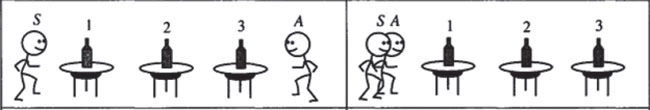
\includegraphics[width=0.8\textwidth]{img/dem2.jpg}
 \end{figure}

Результаты, полученные в ходе этого и следующего экспериментов, представлены в виде таблиц с ответами информантов, где в двух столбцах, представляющих два опыта эксперимента, содержатся данные — демонстративы, употребленные информантами при указании на объекты по пути от ближнего к дальнему. I обозначает I серию, II — II серию, III — III серию демонстративов. По второму эксперименту данные разделены на две таблицы, которые мы будем рассматривать как разные стратегии употребления указательных местоимений. Выделяя основные тенденции и рассматривая каждую парадигму употребления информантом демонстративов как систему, мы перейдем к частным случаям.

\begin{sidewaystable}
 \centering
 \caption{Эксперимент 2}
 \smallskip
 \label{tab:dem2}
 \begin{tabular}{c|c|ccc|ccc} \toprule
 \multirow{2}{*}{{\small стратегия}} &\multirow{2}{*}{{\small \makecell[c]{инфор-\\мант}}} & \multicolumn{3}{c|}{опыт 1} & \multicolumn{3}{c}{опыт 2} \\
 & & {\small объект №1} & {\small объект №2} & {\small объект 3} & {\small объект №1} & {\small объект №2} & {\small объект №3} \\ \midrule
 \multirow{8}{*}{A} & 1 & I & II & II & I & III & III \\
 & 2 & I & II & II & I & II & III \\
 & 3 & I & II & II & I & II & III \\
 & 4 & I & I & II & I & I & III \\
 & 5 & I & II & —* & I & III & III \\
 & 6 & I & II & II & I & III & III \\
 & 7 & I & II & II & I & III & III \\
 & 8 & II & II & II/III & II & II & III \\ \midrule
 \multirow{4}{*}{B} & 9 & I & II & III & I & I & III \\
 & 10 & I & III & III & I & III & III \\
 & 11 & I & II & III & I & I/II & III \\
 & 12 & I & I & III & I & II & III \\ \bottomrule
 \end{tabular}
 \\
 \medskip
 \hspace*{\fill}{\small *Ответ информанта зафиксировать не удалось.}
\end{sidewaystable}

Каждый эксперимент можно представить как поступательное изменение относительно предыдущего. Так, в первом опыте мы имеем картину предыдущего эксперимента, изменённую таким образом, что в расширенное дискурсивное пространство был добавлен ещё один референт. Вместе с тем во втором эксперименте информанты называют все референты, а не только референт №2, как в первом. Таким образом, сначала наша задача состоит в том, чтобы проследить, как меняется употребление УМ носителями при увеличении количества референтов до трёх.

Рассмотрим опыт 1 в рамках стратегии A (Таблица \ref{tab:dem2}). Мы видим доминирующую стратегию маркирования, в которой объект №2 во всех случаях, кроме одного, маркируется демонстративом II серии. Так же употребляется он и в отношении объекта №3 во всех случаях, кроме одного, где ответ информанта не удалось зафиксировать. Применительно к аналогичной ситуации в португальском языке, А.~А.~Ростовцев-Попель пишет о необходимости показать контраст между ближним и сравнительно удалённым объектом \parencite[27]{popiel2009}. Касательно референта, находящегося на наибольшем удалении от говорящего, такой же необходимости различать в указании его и средний референт не возникает. В той же работе рассматривается ситуация, в которой невозможно употребить УМ III серии и при указании на объект, «находящийся во внутреннем пространстве коммуникации», т.~е.~находящийся между локуторами: А.~А.~Ростовцев-Попель признаёт, что языки, которые не допускают такого указания, более склонны к дистантному ориентированию, нежели те, в которых оно возможно \parencite[27]{popiel2009}. Примеров такого употребления в шугнанском нами не выявлено. К той же части таблицы, где употребление демонстративов II серии не встречается вовсе, мы вернёмся позднее.

Теперь обратимся к стратегии B (Таблица \ref{tab:dem2}) для первого опыта. Наглядно в сравнении с данными, рассмотренными выше, употребление информантами демонстративов III серии при указании на референт №3, то есть объект, ближайший к адресату. Так, можно наблюдать, как в первом случае одна часть информантов чётко определяет референт №3 в область адресата (II серия), в то время как другая употребляет в его отношении демонстративы III серии. Употребление последних в шугнанском языке зафиксировано в отношении пространственно удалённых объектов, а в дискурсивном пространстве ассоциируется со сферой 3-го лица, то есть не соотносимой с локуторами \parencite[26]{yusufbekov1998}. Таким образом, информанты, употребившие в данном контексте УМ III серии, склонны игнорировать позицию адресата, отдавая предпочтение параметру удалённости референта №3.

Теперь посмотрим, как отвечали информанты во втором опыте. Если для стратегии A изменение позиции адресата повлекло изменения в указании на референты (принципиален переход от II серии к III в отношении референта №3), то в стратегии B этого не происходит (в двух случаях возможно несколько вариантов УМ, их мы рассмотрим позднее). В таком случае можно сказать, что стратегия B решает проблему появления референта №3 тем, что игнорирует позицию адресата. Ведь всё те же информанты употребляли в ходе первого эксперимента демонстративы II серии, значит, увеличение числа референтов изменило подход к указанию в сторону более дистантно-ориентированного. Исходя из анализа Ростовцева-Попеля, положение адресата в дистантно-ориентированной системе не является опорной точкой при наличии трёх и более референтов \parencite[29]{popiel2009}. Во втором опыте позиции локуторов совпадают, а использование указательных местоимений становится чуть более упорядоченным: абсолютно доминируют УМ I и III серии в указании соответственно на референты №1 и №3.

В указании на референт №2 как в стратегии A, так и в стратегии B используются все три типа маркирования демонстративов (I, II, III), однако принципы их употребления в разных стратегиях разные. Так, в рамках стратегии B, по-видимому, доминирует дистантная ориентация и УМ II серии используется для указания на объект средней удалённости от дейктического центра. В иных случаях для построения дистантной оппозиции употребляются демонстративы только I и III серий — тогда все референты маркируются либо как I–III–III, либо как I–I–III. В ответах этих информантов при появлении третьего референта II серия выходит из употребления, и система работает как двухчастная. Важно подчеркнуть тот факт, что II серия УМ не полностью отсутствует в идиолектах этих информантов, поскольку в первом эксперименте II серию употребляли 100\% участников эксперимента.

За исключением одного случая (информант 4), в стратегии A используется УМ II или III серии для указания на референт №2. Исходя из сугубо дистантного определения шугнанских УМ, III серия употребляется в отношении далёкого, II серия — относительно близкого референта (видимого в обоих случаях) \parencite[40]{yusufbekov1998}. Эта дистантная неопределённость их разграничения, зависимость его от личного отношения говорящего были отмечены в работе \parencite{belikov1972}. Употребить как II, так и III серию можно в одной и той же ситуации:

\pex<exdem3>
\a<a> \begingl
\gla Йам сит-дор жиниҷ, \b{йид} тозā.//
\glc {\sc d1.sg} земля-{\sc hb} снег {\sc d2.sg} чистый//
\endgl
\a<b> \begingl
\gla Йам сит-дор жиниҷ, \b{йу} тозā.//
\glc {\sc d1.sg} земля-{\sc hb} снег {\sc d3.m.sg} чистый//
\glft ‘Этот снег грязный, \b{тот} — чистый.’ \trailingcitation{\parencite[74–75]{belikov1972}}//
\endgl \xe

Объяснить применение разных стратегий в употреблении демонстративов можно через признание идиолектной оппозиции лично- и дистантно-ориентированных дейктических систем. Из рассмотренных А.~А.~Ростовцевым-Попелем языков мы вновь берём португальский как образец: когда во втором опыте теряет значение позиция адресата, в этом языке выходят из употребления УМ II серии, и система становится двухчастной \parencite[28–29]{popiel2009}. Такой же вариант маркирования предлагает и стратегия A во втором опыте (большинство случаев). В иных случаях, где система сохраняет употребление демонстративов II серии, доминирует определение относительно дейктического центра, и последние отсылают не к сфере адресата, а, как это происходит и в стратегии B, указывают на объект, находящийся на среднем удалении от дейктического центра. Таким образом, полученные в результате эксперимента данные подтверждают первоначальное разделение на две группы.

Рассмотрим тот случай в рамках стратегии A, где для указания на ближайшие к говорящему два объекта используются демонстративы I серии (обозначены в двух опытах в Таблице \ref{tab:dem2} как I–I–II и I–I–III — информант 4). Так, использование дейктика II серии в первом опыте (III серии во втором) для обозначения референта №3 уже не позволяет назвать эту систему дистантно-ориентированной: информант учитывает позицию адресата. Возможно, так выглядит несколько нетипичная для шугнанского модель лично-ориентированной системы, где из-за вытеснения II серии I серия частично заняла её «нишу» в дискурсе. Также пограничными можно назвать два случая в Таблице \ref{tab:dem2}. Первый из них (информант 11) обозначен как I–II–III в первом опыте и I–I/II–III во втором. В первом опыте соблюдается выбор демонстративов, типичный для стратегии B, однако, когда положение адресата меняется во втором опыте, появляется вариативность, где при выборе УМ II серии говорящий придерживается стратегии B, но при выборе УМ I серии реагирует на перемещение адресата. Систему, где выбор был совершён в пользу I серии, справедливо считать лично-ориентированной.

Последним нерассмотренным отдельным случаем является информант 8 в Таблице \ref{tab:dem2}: II–II–II/III и II–II–III. Здесь информант допускает повтор в маркировании референта №3 из первого во второй опыт (III~$\rightarrow$~III). Этот повтор совершенно не свойственен стратегии A. В том же месте допускается и типичный для лично-ориентированной стратегии переход II~$\rightarrow$~III. Мы же относим этого информанта к стратегии A из-за выбора демонстративов в маркировании референта №1. Употребление II серии УМ в его отношении не типично ни для одной из стратегий (и более того, ни для одного из информантов в этом эксперименте). Однако выбор II серии говорит больше в пользу личной ориентации, чем дистантной. В дистантно-ориентированной системе употребление II серии объясняется выражением средней степени удалённости от дейктического центра. В данных стратегии B мы видим такие системы, индифферентные к позиции адресата, в них УМ существуют в парадигме «ближний–средний–дальний» или «ближний–дальний», когда система редуцируется до двухчастной. Парадигма «средний–дальний» невозможна для двухчастных систем, ведь двухчастная система предполагает бинарную оппозицию «близко–далеко». В пользу дистантной ориентации здесь можно говорить лишь в том случае, если информант 8 во всех ответах употребляет II серию УМ в значении ближней степени удалённости. В действительности, в речи информанта 8 отсутствуют УМ I серии во всех трёх проведённых экспериментах. Примеров такого замещения в существующих описаниях шугнанского нами не обнаружено, однако полностью исключать этот вариант нельзя.

Иначе объяснить такое проявление II серии можно через вариативность в употреблении демонстративов I и II серий. Существующие описания позволяют предположить определённую свободу в выборе между этими сериями. В действительности, «если говорящий оценивает расстояние между собой и адресатом как “близкое” и наблюдаемый объект находится в поле их зрения, может быть употреблена как I, так и II серия» \parencite[35]{yusufbekov1998}.

\pex<exdem4>
\a<a> \begingl
\gla \b{Дāδ} ту коргар-ен=ен фук=аθ йаст=о?//
\glc {\sc d2.pl} {\sc pron.2sg} рабочий-{\sc pl=3pl} все={\sc int} есть={\sc q}//
\endgl
\a<b> \begingl
\gla \b{Мāδ} ту коргар-ен=ен фук=аθ йаст=о?//
\glc {\sc d1.pl} {\sc pron.2sg} рабочий-{\sc pl=3pl} все={\sc int} есть={\sc q}//
\glft ‘\b{Эти} твои работники все присутствуют?’ \trailingcitation{\parencite[35]{yusufbekov1998}}//
\endgl \xe

Приведённые выше примеры мы взяли у Ш.~П.~Юсуфбекова. Описанный им опыт очень схож с тем, что можно наблюдать во втором опыте второго эксперимента, а также в отношении референта №2 для первого опыта эксперимента. Бригадир, обращаясь к звеньевому, находится вместе с ним в одном дискурсивном пространстве, а работники, о которых первый спрашивает второго, — в другом. Вышерассмотренные примеры говорят нам о существовании пограничных областей коммуникативного пространства, где допустимо употребление как I, так и II серии, как II, так и III серии демонстративов.

Теперь выдвинем предположение о двух стратегиях построения дейктической системы, наблюдаемых в этом эксперименте. Нельзя сказать, что их данные представляют собой безупречную оппозицию: можно наблюдать колебания от более дистантного к более личному пониманию пространства носителем. Однако между ними можно провести чёткую границу, где одна система будет принадлежать стратегии A, а другая — стратегии B (как в примере с тремя УМ II серии, рассмотренном выше — стратегия определяется в зависимости от употребления одного ключевого дейктика). При этом выпадение из употребления УМ II серии и переход системы к двухчастной свойственны обеим стратегиям. В случае стратегии A это происходит из-за исчезновения точки опоры в лице адресата во втором опыте, в случае стратегии B — из-за изначального непринятия во внимание положения адресата. Разделение данных эксперимента на стратегии A и B даёт возможность постулировать лично-дистантную оппозицию в рамках дейксиса шугнанского языка. Таким образом, к стратегии A отнесены те идиолекты, которым свойственна личная ориентация, а к стратегии B те, которым свойственна дистантная. Стратегия A представляется нам более традиционной для шугнанского языка, исходя из вышеупомянутых памироведческих описаний.

Иначе можно было бы представить природу подобного разделения как диалектную, т.~е.~связать её с областью распространения тех или иных языковых явлений. Так, например, М.~Жиц Фукс в своём исследовании дейксиса в хорватском языке находит различия в употреблении демонстративов в зависимости от того, проживает носитель в столичном Загребе или в сельской местности \parencite[55]{zic_fuchs1996}. Такое разделение не представляется нам возможным, поскольку носителей шугнанского, предпочитающих ту или иную стратегию, не удаётся распределить тем же образом в зависимости от происхождения, «образа жизни» или «физического окружения», как то обнаружила для хорватского М.~Жиц Фукс \parencite[60]{zic_fuchs1996}. В Таблице \ref{tab:dem4} представлено распределение ответов информантов и местности их происхождения и проживания. Курсивом отмечены ответы информантов в рамках стратегии B. Не претендуя на статистический анализ, отметим, что данные не позволяют представить какой-либо зависимости выбора стратегии от места. Информанты, происходящие из одного города или джамоата (сельской общины в Таджикистане) или проживающие в одном городе, прибегают к разным стратегиям употребления УМ.

\begin{sidewaystable}
 \centering
 \caption{Результаты эксперимента 2 и места происхождения / проживания информанта}
 \smallskip
 \label{tab:dem4}
 \begin{tabular}{c|ccc|ccc|cc} \toprule
 информант & \multicolumn{3}{c|}{опыт 1} & \multicolumn{3}{c|}{опыт 2} & \makecell{место\\ происхождения} & \makecell{место\\ проживания} \\ \midrule
 3 & I & II & II & I & II & III & Кушк (дж.~Поршинев)* & Хорог \\
 11 & I & II & III & I & I/II & III & Поршинев & Москва и МО* \\
 4 & I & I & II & I & I & III & Вуж (дж.~Вер) & Москва и МО \\
 5 & I & II & — & I & III & III & — & Душанбе \\
 6 & I & II & II & I & III & III & Душанбе & Душанбе \\
 2 & I & II & II & I & II & III & Хорог & Хорог \\
 7 & I & II & II & I & III & III & Хорог & Душанбе \\
 9 & I & I & III & I & I & III & Хорог & Хорог \\
 8 & II & II & II/III & II & II & III & дж.~Дарморахт & Душанбе \\
 10 & I & III & III & I & III & III & Парзудж & Хорог \\
 1 & I & II & II & I & III & III & \makecell{Дашт (дж. Мирсаид\\ Миршакар)} & Дашт \\
 12 & I & II & III & I & II & III & Рошткалинский~дж. & Душанбе\\ \bottomrule
 \end{tabular}
 \\
 \medskip
 \hspace*{\fill}{\small *\i{дж.} — джамоат, МО — Московская область.}
\end{sidewaystable}

\section{Эксперимент третий. Тест на невидимость} \label{dem-exp3}

В основе третьего эксперимента были позиции адресата и говорящего, отличные от опыта 2 второго эксперимента только тем, что референты оказывались у них за спиной, см.~Рисунок \ref{fig:dem3}. Референты были уже «известны» участникам коммуникации из предыдущего эксперимента и становились невидимы для них лишь на этом этапе, что позволяет говорить об анафорическом контексте при их упоминании, как в мнемонических детских играх, где участники определённое время запоминают предметы, а после этого перечисляют их по памяти.

\begin{figure}[H]
 \centering
 \caption{Третий эксперимент \parencite[30]{popiel2009}}
 \smallskip
 \label{fig:dem3}
 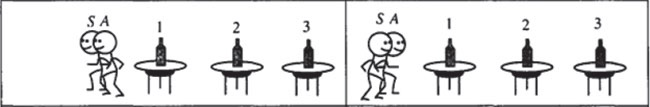
\includegraphics[width=0.8\textwidth]{img/dem3.jpg}
\end{figure}

В Таблице \ref{tab:dem5} приведены результаты эксперимента. Для сравнения также указаны ответы информантов в последнем опыте второго эксперимента, когда локуторы стоят лицом к ряду объектов (он же на второй половине рисунка \ref{fig:dem3}). \b{Жирным} выделены те случаи, где выбор местоимения не зависит от видимости~/~невидимости референта.

\begin{table}[h]
 \centering
 \caption{Результаты эксперимента 3}
 \smallskip
 \label{tab:dem5}
 \begin{tabular}{c|ccc|ccc} \toprule
 информант & \multicolumn{3}{c|}{эксперимент 3} & \multicolumn{3}{c}{\makecell{эксперимент 2\\ (опыт 2)}} \\ \midrule
 1 & III & III & III & I & III & III \\
 2 & \b{I} & \b{II} & \b{III} & \b{I} & \b{II} & \b{III} \\
 3 & \b{I} & \b{II} & \b{III} & \b{I} & \b{II} & \b{III} \\
 4 & I & III & III & I & I & III \\
 5 & II & III & III & I & III & III \\
 6 & II/III & III & III & I & III & III \\
 7 & II & III & III & I & III & III \\
 8 & II & III & III & II & II & III \\
 9 & \b{I} & \b{I} & \b{III} & \b{I} & \b{I} & \b{III} \\
 10 & \b{I} & \b{III} & \b{III} & \b{I} & \b{III} & \b{III} \\
 11 & I & II/III & III & I & I/II & III \\
 12 & II & II & II/III & I & II & III\\ \bottomrule
 \end{tabular}
 \\
 \medskip
\end{table}

\pagebreak[4]

Сразу следует отметить, что мы не разделяем данные третьего эксперимента на отдельные стратегии употребления демонстративов. В том числе то разделение, что имело место в рамках предыдущего эксперимента, здесь не сохраняется. Однако представляется возможным выделить несколько групп УМ, имеющих общие подходы к реализации дискурса.

Первой такой группой можно назвать ту, в рамках которой употребление демонстративов не зависит от видимости/невидимости референтов (4 случая). В их число входят системы, тяготеющие как к личной, так и к дистантной ориентации.

Однако системы идиолектов, наиболее устремлённые к личной ориентации, в эту группу не входят. Критерием выделения таковых стало исчезновение из употребления II серии УМ при совпадении позиций говорящего и адресата во втором эксперименте (информанты 1, 4, 5, 6, 7). Мы знаем, что УМ III серии употребляются как исключения как из сферы адресата, так и из сферы говорящего и имеют семантику удалённости \parencite[32]{yusufbekov1998}. Таким же образом, по-видимому, исключаются референты из пространства речевого акта, оказываясь невидимыми. Для двух информантов из этой группы (информанты 1 и 6) существует способ маркирования, заключающийся в употреблении УМ III серии относительно всех референтов. Этот способ маркирования (III–III–III), засвидетельствованный в речи двух носителей, имеет типологическое сходство с дейктической системой португальского языка, отмечаемой А.~А.~Ростовцевым-Попелем в том же контексте \parencite[30]{popiel2009}. Речи информантов 4, 8 и 11 также свойственен сдвиг I~$\rightarrow$~III или II~$\rightarrow$~III — с той разницей, что он не приводит к маркированию всех референтов III серией УМ. На основании ответов этих пяти информантов выделим вторую группу, в которой стимул невидимости вызывает маркирование референтов при помощи III серии УМ.

Третью группу мы выделим из тех примеров, где реакцией на невидимость референтов стал сдвиг в сторону II серии (I~$\rightarrow$~II и III~$\rightarrow$~II). К ней можно отнести ответы информантов 5, 6, 7, 11, 12. Заметим, что идиолекты одних и тех же информантов (6, 11) допускают отнесённость как ко второй, так и к третьей группе. В свою очередь, у Ш.~П.~Юсуфбекова есть пример употребления УМ I и II серии в схожем контексте. Говорящий сидит спиной к окну и задаёт вопрос (\getfullhref{exdem5.a}), его собеседник, напротив, наблюдает за происходящим снаружи (\getfullhref{exdem5.b}):

\pex<exdem5>
\a<a> \begingl
\gla — Ар \b{дам} мāш кийоска=йен ку газӣт вӯɣ̌ҷ=о, ~~~~~~ йид ғал чуст?//
\glc ~~~~~~ {\sc down} {\sc d2.f.sg.o} {\sc pron.1pl} киоск={\sc 3pl} {\sc ptcl} газета нести.{\sc pf=or} ~ {\sc d2.sg} ещё закрытый//
\glft ‘Привезли ли в \b{(э)тот} (II~серия) наш киоск газеты, или он ещё закрыт?’//
\endgl
\a<b> \begingl
\gla — \b{Йам}=и йет чӯɣ̌ҷ=ат, газӣт=ен ~~~~~~~~~~~~~~~~~~~ ғал гуму̊н на-вӯɣ̌ҷ.//
\glc ~~~~~~ {\sc d1.sg=3sg} открытый делать.{\sc pf=and2} газета={\sc 3pl} ~ ещё видимо {\sc neg}-нести.{\sc pf}//
\glft ‘\b{Этот} (I~серия) [киоск] уже открыт, но газеты, видимо, ещё не привезли.’ \trailingcitation{\parencite[39]{yusufbekov1998}}//
\endgl \xe

Здесь существуют два критерия разграничения I и II серий: во-первых, это «видимость/невидимость определяемого объекта для говорящего и собеседника (т.~е.~видимое выступает как близкое, невидимое воспринимается как далёкое)» \parencite[39]{yusufbekov1998}, во-вторых, упоминается субъективная точка зрения говорящего, вызванная его отличным от адресата местоположением. Поскольку же в третьем эксперименте позиции говорящего и адресата совпадают, внимание здесь следует сосредоточить на первом критерии.

В свою очередь переход III~$\rightarrow$~II, наблюдаемый в идиолекте информанта 12 в контексте третьего эксперимента, с трудом поддаётся объяснению через дейктическое противопоставление, ведь II серия УМ в оппозиции II~\textasciitilde~III серий отвечает за условно более близкий объект, находящийся в пространстве, соотносимом с собеседником. Эти данные заставляют нас обратиться к определению II серии как общеуказательной. Тенденцию к утрате у II серии УМ значения указания на сферу собеседника и возникновение оппозиции II~\textasciitilde~III серий по наличию у II серии «значения подчёркнутого указания» и отсутствия такового у III серии отмечает Ш.~П.~Юсуфбеков [\cite*[41]{yusufbekov1998}]. Наша уверенность в употреблении II серии УМ здесь в значении общеуказательной основывается на ряде причин. Во-первых, в эксперименте 3 данные информанта 12 дают нам систему, где все референты маркируются II серией. Это подтверждает отсутствие противопоставления из-за удалённости референтов друг от друга и от дейктического центра. Во-вторых, мы определили дейктик II серии как немаркированный компонент в шугнанской системе. Из этого следует, что употребление II серии информантом в таком контексте (II–II–II) недейктическое, оно не маркирует удалённость от дейктического центра, однако указывает на значение дейктика II серии как дейктика «по умолчанию».

\pagebreak[2]

С целью исключить, возможно, слишком навязчивую интерпретацию пространственного определения референтов в парадигме «ближний–средний–дальний», мы включили в систему четвёртый референт и провели дополнительный эксперимент. В него были включены два опыта, необходимые для решения нашей задачи: первый — опыт 2 второго эксперимента, но с четырьмя объектами вместо трёх, второй — опыт третьего эксперимента с четырьмя объектами вместо трёх (см.~Рисунок \ref{fig:dem3}). В Таблице \ref{tab:dem6} представлены ответы информантов: в них абсолютно преобладает употребление II серии УМ. Только в одном случае информант 2 не указал на второй по удалённости референт с помощью II серии, однако допустил возможность такого указания. Этот эксперимент даёт нам большее представление о II серии как общеуказательной. Возможно, когда количество референтов, расположенных на приблизительно одинаковом удалении, становится больше трёх, необходимость в дейктическом противопоставлении этих объектов резко отпадает.

\begin{table}
 \centering
 \caption{Результаты дополнительного эксперимента}
 \smallskip
 \label{tab:dem6}
 \begin{tabular}{c|cccc|cccc} \toprule
 информант & \multicolumn{4}{c|}{опыт 1} & \multicolumn{4}{c}{опыт 2} \\ \midrule
 1 & II & II & II & II & I/II & II & II & II \\
 2 & II & II & II & II & II & II & III(II) & II\\ \bottomrule
 \end{tabular}
 \\
 \medskip
\end{table}

Сделаем выводы по третьему эксперименту. Основное разделение по третьему эксперименту — наличие или отсутствие реакции на стимул невидимости. Противопоставление лично- и дистантно-ориентированных систем в этом контексте не даёт нам такого чёткого разделения, как в предыдущем эксперименте, однако членение на отдельные меньшие группы в данных сохраняется. В первую группу мы выделили системы, где фактор невидимости информантами игнорировался. Во вторую и третью группы вошли идиолекты, в которых невидимость референтов стала стимулом для большего употребления III и II серии УМ соответственно. Мы видим, что шугнанский дейксис допускает определённые способы маркирования невидимых референтов, но нельзя сказать, что какой-то один из них доминирует.

Теперь, опираясь на вышеперечисленные примеры, обратим внимание на данные К.~Мюллер. В работе \parencite{muller2015} шугнанские УМ группируются по степени удалённости от говорящего: ближней, средней и дальней соответственно; это местоимения \i{ми}/\i{мам}/\i{мāδ}, \i{ди}/\i{дам}/\i{дāδ} и \i{wи}/\i{wам}/\i{wāδ} \parencite[57]{muller2015}. УМ \i{йам} и \i{йид} указаны как детерминативы с дейктическими функциями: \i{йам} указывает на ближнюю область в рядом с говорящим, \i{йид} на ближнюю область в пространстве непосредственно перед говорящим \parencite[59]{muller2015}. Однако ещё по примерам (\gethref{exdem6})–(\gethref{exdem7}) \parencites[74–77]{belikov1972}[22]{yusufbekov1998} можно установить, что \i{йам} и \i{йид} употребляются как демонстративы и не требуют после себя именной группы, как это делают детерминативы. К демонстративам \i{йам} и \i{йид} относит в своей классификации и М.~Аламшоев [\cite*[31]{alamshoev1994}].

\ex<exdem6>
\begingl
\gla Йу=йи бāд дараw бирêх̌т су̊д, ~~~~~~~~~~~~~~~~~~~~~~~~~~~~~~~~~~~~ ху лу̊в-ҷ=и: «Аҷаб ба-маза на-вад? ~~~~~~~~~~~~ Ду̊нд ик=га рӯған ца вед, \b{йам} соф-аθ ба-маза су̊д».//
\glc {\sc d3.m.sg=3sg} потом {\sc inc} пить.{\sc inf} стать.{\sc prs.3sg} ~ {\sc and1} говорить-{\sc pf=3sg} {\sc ptcl} {\sc all}-вкус {\sc neg}-быть.{\sc pst.f/pl} ~ столько {\sc emph=add} масло {\sc subd} быть.{\sc prs.3sg} {\sc d1.sg} совсем-{\sc adv} {\sc all}-вкус стать.{\sc prs.3sg}//
\glft ‘И он потом начал пить и сказал: «[Разве] не удивительно вкусно? Ещё немного масла было бы, \b{это} стало бы совсем вкусно».’ \trailingcitation{\parencite[75]{belikov1972}}//
\endgl \xe

\ex<exdem7>
\begingl
\gla — Бийор=ам цу̊нд ту х̌икӯд, ~~~~~~~~~~~~~~~~~~~ на-вӯд=āм ту. ~~~~~~~~~~~~~~~~~~~~~~~~~~~~~~~~~~~~~~~~~~~~~~~~~~~~~~~~~~~~~~~~~~~~~~~~~~~~ — Цу̊нд=анд вуд \b{йид}?//
\glc ~~~~~~ вчера={\sc 1pl} сколько {\sc pron.2sg} искать.{\sc pst} ~ {\sc neg}-найти.{\sc pst=1pl} {\sc pron.2sg} ~ ~~~~~~ сколько={\sc loc} быть.{\sc pst.m.sg} {\sc d2.sg}//
\glft ‘— Вчера столько тебя искали, но не нашли. — Во сколько было \b{это}?’ \trailingcitation{\parencite[22]{yusufbekov1998}}//
\endgl \xe

На рассмотренном выше примере (\gethref{exdem5}), а также на основании обозначенных выше контекстов употребления II серии УМ мы видим, что соотнесение \i{йид} с сугубо ближней областью в пространстве перед говорящим у Мюллер [\cite*[59]{muller2015}] не раскрывает всю вариативность употребления этого местоимения в шугнанском языке. Из выводов Мюллер [\cite*[60]{muller2015}] также следует, что употребление местоимений \i{ми}/\i{мам}/\i{мāδ}, \i{ди}/\i{дам}/\i{дāδ} — I и II серии соответственно — невозможно в контекстах невидимости. Из полученных нами данных эксперимента 3 можно выделить систему, которая действительно работает таким образом (идиолект информанта 1). Несомненно, способ маркирования невидимых референтов при помощи III серии существует. Однако, исходя из того же примера (\gethref{exdem5}), а также совокупности данных, полученных нами в ходе эксперимента, мы можем опровергнуть эти выводы К.~Мюллер.

\section{Заключение} \label{dem-conclusion}

В ходе нашего исследования была установлена большая вариативность в построении дейктических систем в шугнанском языке. Это связано с разнонаправленными стратегиями, применявшимися носителями в ходе экспериментов. Первый эксперимент позволил нам установить немаркированный компонент в шугнанской системе — II серию УМ, при этом его данные были лишены даже единичных отклонений. Такое определение II серии УМ коррелирует с её значением подчёркнутого указания. Результаты второго эксперимента подтверждают существование личной и дистантной оппозиции в языке. Мы установили две стратегии употребления демонстративов в данном контексте, где принципом разделения является наличие или отсутствие реакции носителя на смену положения адресата в пространстве. Третий эксперимент позволил выявить способы маркирования невидимых объектов. Его данные представляются наиболее вариативными, вместе с этим разделение на группы в третьем эксперименте не соответствует разделению на две стратегии во втором эксперименте. Также мы склонны считать, что природу вариативности систем нельзя объяснить диалектным территориальным членением, так как приведённая нами география распространения явлений не даёт нам для этого никаких оснований. Дистантная ориентация в контексте трансформации системы в двухчастную, засвидетельствованная в проведённых нами экспериментах, не была отмечена ранее в описаниях шугнанского языка. В свою очередь, определение УМ только через парадигму удаленности «ближний–средний–дальний» в не в полной мере отражает семантику трёхчастных систем. Также и в шугнанском, факторы видимости, соотнесённости со сферами говорящего и адресата, а также количества объектов референции влияют на употребление того или иного УМ и создают основания для внутриязыковой вариативности.

\chapter*{Эвиденциальный Перфект в~шугнанском языке}
\addcontentsline{toc}{chapter}{\textit{М.~Меленченко}. \textbf{Эвиденциальный Перфект в~шугнанском языке}}
\setcounter{section}{0}
\chaptermark{Эвиденциальный Перфект в~шугнанском языке}
\label{chapter-melen-evid}

\begin{customauthorname}
Максим Меленченко
\end{customauthorname}

\begin{englishtitle}
\i{Evidential Perfect in Shughni\\{\small Maksim Melenchenko}}
\end{englishtitle}

\begin{abstract}
В статье с семантической точки зрения рассматривается одна из видовременных форм шугнанского языка, традиционно именуемая Перфектом. Эта форма имеет много ареально-типологических сходств с перфектами в других языках Западной и Центральной Азии. В частности, шугнанский развил эвиденциальное противопоставление между Претеритом и Перфектом, в котором Перфект используется для незасвидетельствованных событий. Он также выражает экспериенциальную и ирреальную семантику. Выделяется небольшой класс «стативно-перфектных» глаголов, у которых форма Перфекта выражает состояние в настоящем. Кроме того, в статье анализируются «миративные» употребления глагола ‘быть’ в форме Перфекта, а также употребление перфектных форм в нарративах.
\end{abstract}

\begin{keywords}
время, иранские языки, миративность, памирские языки, перфект, шугнанский язык, эвиденциальность.
\end{keywords}

\begin{eng-abstract}
This paper describes the semantics of one of the verb forms in Shughni, traditionally called Perfect. This form displays many areally-motivated typological similarities with perfects in other languages of Western and Central Asia. In particular, Shughni has developed an evidential opposition between the Preterite and the Perfect, in which the Perfect is used for non-witnessed events. It is also used to express experiential and irreal semantics. A small class of “stative-perfect” verbs is distinguished, for which the Perfect form expresses a state in the present. In addition, the article analyzes so-called “mirative” uses of the Perfect of the copula, as well as the use of Perfect forms in narratives.
\end{eng-abstract}

\begin{eng-keywords}
evidentiality, Iranian, mirativity, Pamir area, perfect, Shughni, tense.
\end{eng-keywords}

\begin{acknowledgements}
Автор выражает глубокую благодарность Сильвии Лураги, С.~К.~Михайлову, В.~А.~Плунгяну и К.~В.~Филатову за ценные советы, комментарии и обсуждения, а также всем шугнанским консультантам, в особенности Мадине Ардабаевой и Амригул Шоназаровой. Публикация подготовлена в ходе проведения исследования (проект №~22-00-034) в рамках Программы «Научный фонд Национального исследовательского университета “Высшая школа экономики” (НИУ~ВШЭ)» в 2023~году.
\end{acknowledgements}

\begin{initialprint}
\fullcite{melenchenko2023_evidential}\end{initialprint}

\section{Введение} \label{evid-intro}

Перфект~— глагольная категория, с трудом поддающаяся единообразной типологической характеристике. Для европейских языков его семантика традиционно описывается в терминах понятий «\textbf{результат}» или «\textbf{текущая релевантность}» \parencite[52–65]{comrie1976}. Кроме того, одним из наиболее частотных значений, выражаемых перфектами, является экспериенциальность~— указание на опыт в прошлом без привязки к конкретному событию \parencite[67]{bybee_dahl1989}. Так, в посвящённой перфектам главе в атласе WALS перфектами считаются только формы, которые имеют и значение результата, и экспериенциальное значение \parencite{dahl_velupillai2013}.

У языков Западной и Центральной Азии, включая многие иранские, тюркские и уральские языки, а также языки Кавказа, одним из наиболее частотных значений перфекта зачастую является \textbf{непрямая эвиденциальность} \parencites[93]{lazard1999}[375]{lindstedt2000}. Этот ареал также известен как Большой эвиденциальный пояс \parencite[14–15]{plungian2016}. Известно, что перфекты часто развиваются из результативных причастий \parencites[68–69]{bybee_etal1994}[367–373]{lindstedt2000}, однако они характеризуются диахронической нестабильностью и поэтому сами легко подвергаются семантическому сдвигу. Они могут заменить обычное прошедшее время~— этот известный феномен называют «аористическим сдвигом»~— или же приобрести те самые эвиденциальные значения и постепенно грамматикализоваться в специализированный показатель эвиденциальности \parencite[95–97]{bybee_etal1994}. По-видимому, в первую очередь перфект начинает использоваться для событий, о которых говорящий узнаёт путём логического вывода («инферентив»), а уже потом может расшириться до событий, о которых говорящий узнаёт от другого человека («репортатив»). По словам С.~Ферхеес, семантический сдвиг в сторону эвиденциальности вызван сменой направления каузальной импликатуры, присущей результативу: если имеется видимый результат, то ему должно соответствовать событие в прошлом \parencite[78]{verhees2019}. Так по результату человек достраивает картину прошлого, которое он не наблюдал,~— это и есть инферентивное значение.

Настоящая статья представляет собой описание семантики Перфекта в шугнанском языке, который принадлежит к шугнано-рушанской подгруппе внутри восточноиранских языков. Шугнанский также включается в памирские языки~— ареальное объединение внутри восточноиранской группы. На нём говорит около 90~000 человек в Таджикистане и Афганистане \parencite[787–788]{edelman_dodykhudoeva2009_shughni}. Как и многие другие иранские языки, шугнанский развил способ выражения эвиденциального статуса событий в прошлом с помощью видовременных форм глагола. В основном форма Перфекта используется для выражения незасвидетельствованных событий, в то время как для выражения засвидетельствованных событий используется Претерит. В статье описываются особенности употребления шугнанского Перфекта. Используемые данные получены преимущественно от носителей шугнанского в г.~Хорог (Таджикистан) и в Москве в 2022–2023~годах, также использовались данные из корпуса шугнанского языка\fn{Корпус доступен по ссылке: \i{\href{https://linghub.ru/shughni_corpus/search}{linghub.ru/shughni\_corpus/search}}. Подробнее о корпусе см.~в работе \parencite{makarov_etal2022}. На момент проведения исследования в корпусе содержалось 72 текста общим объёмом более 55~000 словоформ. Для анализа нарративов использовались 18~нарративов из корпуса~— это сказки и истории из письменных источников (13), устные тексты, записанные в экспедициях, (4) и фрагменты перевода Евангелия от Луки.} и электронной версии \parencite{makarov_etal2022} словаря Д.~К.~Карамшоева [\cite*{karamshoev1988}].

В \hyperref[evid-verb]{разделе~2} описывается глагольная система шугнанского языка. В \hyperref[evid-sem]{разделе 3} детально описана семантика шугнанского Перфекта. Собранный материал показывает, что основным значением Перфекта является эвиденциальность (\hyperref[evid-evid]{подраздел~3.1}). При этом он также имеет экспериенциальные (\hyperref[evid-exper]{подраздел~3.2}) и контрфактические употребления (\hyperref[evid-modal]{подраздел~3.5}), а для небольшого числа глаголов имеет только результативно-стативное значение (\hyperref[evid-result]{подраздел~3.3}). В \hyperref[evid-be]{подразделе~3.4} обсуждаются особые употребления глагола бытия в форме Перфекта, а в \hyperref[evid-narr]{подразделе~3.6}~— использование Перфекта в нарративах. В \hyperref[evid-conclusion]{разделе~4} делаются выводы и обобщения.

\section{Глагольная система шугнанского языка} \label{evid-verb}

Шугнанский язык обладает сравнительно простой видовременной системой, в которой выделяются три основных формы: Презенс (также непрошедшее или настояще-будущее), Претерит (или прошедшее) и Перфект. Есть также нефинитные, неиндикативные, а также образованные от основных формы (Плюсквамперфект, Императив, Инфинитивы и различные причастия). Все эти формы синтетические; аналитические глагольные формы в шугнанском обычно не выделяются\fn{Имеется ряд аналитических конструкций~— например, две конструкции с инцептивным значением \parencite[352]{parker2023}~— но традиционно они не включаются в глагольную парадигму.}. Глаголы имеют три основы, которые различают разные формы~— Презенс, Претерит и Перфект. Основы Претерита и Перфекта образуются от основы Презенса с помощью специальных суффиксов; при этом у многих глаголов все три основы также различаются нерегулярными чередованиями в корне. У многих глаголов в Претерите и Перфекте различаются две основы: для мужского рода единственного числа и для женского рода или множественного числа. Основа Претерита всегда маркируется суффиксом -\i{т}/-\i{д}, а Перфектная основа маркируется суффиксом -\i{ц}/-\i{ӡ} для формы женского рода или множественного числа, а во всех остальных случаях (в мужском роде или когда род и число не различаются) используется суффикс -\i{ч}/-\i{ҷ}. Кроме того, у многих глаголов имеется особая форма для 3 лица единственного числа Презенса. См.~Таблицу \ref{tab:evid1}\fn{Примеры из шугнанского и близкородственного ему бартангского приводятся в рабочей латинской транскрипции, примеры из других языков~— в орфографиях, используемых в соответствующих источниках.}:

\begin{table}[h]
 \centering
 \caption{Основные формы четырёх шугнанских глаголов}
 \smallskip
 \label{tab:evid1}
 \begin{tabular}{cc|cccc} \toprule
 \multicolumn{2}{c|}{форма глагола} & ‘бросить’ & ‘дать’ & ‘быть’ & ‘уйти’ \\ \midrule
 \multirow{2}{*}{\makecell{основа\\Презенса {[}{\sc prs}{]}}} & {\small обычная} & \multirow{2}{*}{\i{питêw}-} & \i{δāδ}- & \multirow{2}{*}{\i{ви}-} & \i{ти}- \\
  & {\sc 3sg} &  & \i{δӣ}- &  & \i{тӣз}- \\ \midrule
 \multirow{2}{*}{\makecell{основа\\Претерита {[}{\sc pst}{]}}} & {\sc m.sg} & \multirow{2}{*}{\i{питêw-д}} & \multirow{2}{*}{\i{δо.д}} & \i{ву.д} & \i{тӯй.д} \\
  & {\sc f.sg/pl} &  &  & \i{ва.д} & \i{той.д} \\ \midrule
 \multirow{2}{*}{\makecell{основа\\Перфекта {[}{\sc pf}{]}}} & {\sc m.sg} & \multirow{2}{*}{\i{питêw-ҷ}} & \multirow{2}{*}{\i{δоδ.ҷ}} & \i{вуδ.ҷ} & \i{тӯй.ҷ} \\
  & {\sc f.sg/pl} &  &  & \i{ви.ц} & \i{тӣ.ц} \\ \bottomrule
 \end{tabular}
\end{table}

В форме Презенса глаголы согласуются с субъектом клаузы с помощью лично-числовых окончаний (\gethref{exevid1})\fn{Здесь и далее примеры без указания источника получены от носителей путем элицитации.}. В Претерите и Перфекте основа используется без окончаний, но глагол согласуется с субъектом с помощью лично-числовых энклитик, которые обычно присоединяются к первой именной группе клаузы\fn{Показатель 3 лица единственного числа =\i{и} используется только при переходных и псевдопереходных глаголах [\hyperref[chapter-chist-clitic]{Чистякова 2022b}].} (\gethref{exevid2}); эти же энклитики используются с именными предикатами (\gethref{exevid24}) \parencite[22–31]{chistiakova2021}. Лично-числовые суффиксы и энклитики перечислены в Таблице \ref{tab:evid2}.

\ex<exevid1>
\begingl
\gla Йā ар руз китоб \b{х̌ойд}.//
\glc {\sc d3.f.sg} каждый день книга читать.{\sc prs.3sg}//
\glft ‘Она \b{читает} книгу каждый день.’//
\endgl \xe

\ex<exevid2>
\begingl
\gla Йā=йи wам китоб \b{х̌êй-ҷ}.//
\glc {\sc d3.f.sg=3sg} {\sc d3.f.sg.o} книга читать-{\sc pf}//
\glft ‘[Я вижу, что закладка лежит в самом конце книги:] Она \b{прочитала} эту книгу.’//
\endgl \xe

\begin{table}[H]
 \centering
 \caption{Шугнанские лично-числовые показатели}
 \smallskip
 \label{tab:evid2}
 \begin{tabular}{l|cccccc} \toprule
  & {\sc 1sg} & {\sc 2sg} & {\sc 3sg} & {\sc 1pl} & {\sc 2pl} & {\sc 3pl} \\ \midrule
 \makecell[c]{лично-числовые\\суффиксы в~Презенсе} & -\i{ум} & -\i{и} & -\i{т} / -\i{д} & -\i{āм} & -\i{ет} & -\i{ен} \\ \midrule
 \makecell[c]{лично-числовые\\энклитики, использующиеся\\с~Претеритом и~Перфектом} & =\i{ум} & =\i{ат} & =\i{и} / $\emptyset$ & =\i{āм} & =\i{ет} & =\i{ен} \\ \bottomrule
 \end{tabular}
\end{table}

От основы Перфекта с помощью суффикса -\i{ат} регулярно образуется форма Плюсквамперфекта, при этом лицо и число выражается так же, как и в Перфекте~— энклитиками. В современном языке Плюсквамперфект не употребляется в прототипическом для этой категории значении предшествования в прошлом и сохранил исключительно модальные употребления (\gethref{exevid3})\fn{О семантике формы Плюсквамперфекта см.~более позднюю работу \parencite{melenchenko2025_pluperfect}~— \i{прим.~переиздания}.}.

\ex<exevid3>
\begingl
\gla Кошга=йāм мāш йак-ҷо зиндаги \b{чӯɣ̌ҷ-ат}!//
\glc если\_бы={\sc 1pl} {\sc pron.1pl} один-место жизнь делать.{\sc pf-pqp}//
\glft ‘Вот бы мы \b{жили} вместе!’//
\endgl \xe

Кроме того, от основы Перфекта образуются два причастия: результативное с суффиксом -\i{ин} (\gethref{exevid4}) и пассивное с суффиксом -\i{ак} (\gethref{exevid5}) \parencite[798–799]{edelman_dodykhudoeva2009_shughni}.

\ex<exevid4>
\begingl
\gla <…> Йу̊д-анд ик=дис \b{нивиш-ч-ин}: <…>.//
\glc ~~~~~~ {\sc d1-loc} {\sc emph}=такой писать-{\sc pf-ptcp1} ~~~~~~//
\glft ‘<И сказал им:> так \b{написано}, <и так надлежало пострадать Христу, и воскреснуть из мёртвых в третий день.>’ \trailingcitation{[Лк. 24:46]}//
\endgl \xe

\ex<exevid5>
\begingl
\gla Wāδ=ен ту-рд \b{δоδҷ-ак} сат.//
\glc {\sc d3.pl=3pl} {\sc pron.2sg-dat} дать.{\sc pf-ptcp2} стать.{\sc pst.f/pl}//
\glft ‘Они [уже] \b{даны} тебе.’ \trailingcitation{\parencite{karamshoev1988}}//
\endgl \xe

\pagebreak[4]

С диахронической точки зрения основы Претерита с суффиксом -\i{т}/-\i{д} восходят к древнеиранским причастиям на *-\i{ta}, *-\i{tī} \parencite[77]{dodykhudoeva1988}. Они превратились в «простое» прошедшее время и, в свою очередь, послужили основами для развития вторичных причастий, которые превратились в современный Перфект. Показатели Перфекта -\i{ч}/-\i{ҷ} и -\i{ц}/-\i{ӡ} происходят от суффиксов *-\i{ka} и *-\i{čī}, которые образовывали эти вторичные причастия \parencites[193–203]{pakhalina1989}[290–291]{jugel2020}. По предположению Эдельман [\cite*[358–372]{edelman1975_tense}], формы, соответствующие современному Претериту, могли функционировать как перфекты~— до тех пор, пока появление вторичных причастий на *-\i{ka} не вытеснило их в сферу «простого» прошедшего. Древнеиранские причастия, вероятно, прошли через «перфектный цикл», в котором процесс развития перфекта и последующий «аористический сдвиг» повторяются несколько раз \parencite[24]{plungian2016}. Таким образом, с точки зрения происхождения шугнанский Перфект весьма типичен~— он образовался из результативного причастия. Вместе с тем, по сравнению со многими другими перфектами Большого эвиденциального пояса он выделяется тем, что не задействует связку (глагол бытия)\fn{Впрочем, как справедливо заметил редактор выпуска [журнала «Вопросы языкознания»~— \i{прим.~переиздания}] О.~И.~Беляев, лично-числовые клитики можно считать связками, хотя этот вопрос требует отдельного рассмотрения.}~— а например, в таких языках, как таджикский, болгарский или багвалинский, перфекты в разной степени её задействуют. Однако исторически, по-видимому, Перфект имел по крайней мере нулевую связку. Это косвенно подтверждается устройством формы Плюсквамперфекта в шугнано-рушанских языках, которая происходит из конструкции Перфекта и глагола ‘быть’ в форме Претерита. Например, в близкородственном бартангском языке Плюсквамперфект сохранился именно в таком виде: \i{аз=ум суч вуд} (\textsc{pron.1sg=1sg} идти.{\textsc{pf.m.sg} быть.{\textsc{pst.m.sg}) ‘я ходил’, однако в шугнанском формы \i{вуд}/\i{вад} превратились в суффикс -\i{ат}: \i{уз=ум суδҷ-ат} ({\textsc{pron.1sg=1sg} идти.{\textsc{pf.m.sg-pqp}) ‘я ходил бы’ \parencite[76]{dodykhudoeva1988}. Таким образом они стали синтетическими формами, не встраивающимися в парадигму относительно Презенса и Претерита.

Семантика видовременных форм шугнанского языка до недавнего времени была описана сравнительно слабо. Существующие грамматики и очерки не отличаются разнообразием мнений и формулировок по этой теме. Известно, что Презенс используется для описания событий в настоящем и будущем (для референции к будущему часто используется энклитика =\i{та} \parencite[337–342]{parker2023}). Две формы, Претерит и Перфект, используются для описания событий в прошлом. Претерит в научных работах обычно описывается как «стандартное» прошедшее, не маркированное ни по аспекту, ни по эвиденциальному статусу \parencites[154]{karamshoev1963}[370]{edelman1975_tense}[806]{edelman_dodykhudoeva2009_shughni} (исключение составляет предстоящая грамматика \parencite[346]{parker2023}\fn{Шугнанская грамматика К.~Паркера \parencite{parker2023} ещё не была опубликована на момент написания этой статьи~— \i{прим.~переиздания}.}). Перфект, с другой стороны, обычно считается формой с более специфической семантикой. Пять источников единогласно приписывают ему два значения: одно традиционное для перфекта («наличный результат», «текущая релевантность»), а другое~— эвиденциальное (иногда подразделяющееся на инферентив и репортатив) \parencites[161–162]{karamshoev1963}[39]{pakhalina1969_pamir}[370]{edelman1975_tense}[42–43]{bakhtibekov1979}[806]{edelman_dodykhudoeva2009_shughni}. Значение характеристик типа «результат» и «текущая релевантность», используемых в этих работах, не вполне ясно. На мой взгляд, вполне вероятно, что на эти описания влияли представления их авторов о том, какие значения перфекты выражают в других языках (в том числе в других иранских). Никакие другие «перфектные» значения, встречающиеся в типологической литературе, в этих источниках не упоминаются.

\section{Семантика шугнанского Перфекта} \label{evid-sem}

\subsection{Эвиденциальность} \label{evid-evid}

Для большинства глаголов Перфект, по-видимому, является в первую очередь «эвиденциальным» прошедшим временем. Претерит используется в контекстах прямой засвидетельствованности (\gethref{exevid6}), в то время как Перфект используется в инферентивных (\gethref{exevid7}) и репортативных (\gethref{exevid8}) контекстах. Важно отметить, что в примерах (\gethref{exevid7}) и (\gethref{exevid8}) использование формы Претерита носители считают некорректным. Это показывает, что Претерит всё же маркирован по эвиденциальному статусу события и выражает только прямой доступ говорящего к информации, а Перфект выражает косвенный доступ говорящего к информации (инферентивный или репортативный).

\ex<exevid6>
\begingl
\gla Уз=ум тар мактаб тоқ \#вирух̌-ч / \b{вирух̌-т}, <…>.//
\glc {\sc pron.1sg=1sg} {\sc eq} школа окно ломать-{\sc pf} ~~~~~~ ломать-{\sc pst} ~~~~~~//
\glft ‘Я \b{разбил} окно в спортзале, <и теперь моих родителей вызывают в школу>.’//
\endgl \xe

\ex<exevid7>
\begingl
\gla Ар.чāй.ца аз дев талабā-йен=ен тоқ \b{вирух̌-ч} / \#вирух̌-т.//
\glc каждый {\sc el} {\sc d2.pl.o} ученик-{\sc pl=3pl} окно ломать-{\sc pf} ~~~~~~ ломать-{\sc pst}//
\glft ‘[Учительница слышит звук, заходит в спортзал, видит разбитое стекло и идёт в кабинет директора, чтобы сообщить:] Один из этих учеников \b{разбил} окно.’//
\endgl \xe

\ex<exevid8>
\begingl
\gla Йу=йи тар мактаб хейх̌ā \b{вирух̌-ч} / \#вирух̌-т.//
\glc {\sc d3.m.sg=3sg} {\sc eq} школа стекло ломать-{\sc pf} ~~~~~~ ломать-{\sc pst}//
\glft ‘[Учительница звонит матери подростка и сообщает, что её сын разбил окно в школе. Положив трубку, мать говорит своему мужу:] Он \b{разбил} окно в школе.’//
\endgl \xe

По-видимому, Претерит и Перфект противопоставляют по эвиденциальному статусу не только предельные (\gethref{exevid7})–(\gethref{exevid8}), но и непредельные глаголы, что показывают примеры (\gethref{exevid9}) и (\gethref{exevid10}):

\ex<exevid9>
\begingl
\gla Уз=ум то вегā=йец тар дарго \b{ред}.//
\glc {\sc pron.1sg=1sg} {\sc lim1} вечер={\sc lim2} {\sc eq} двор остаться.{\sc pst}//
\glft ‘[Я забыла ключи от дома.] Я \b{простояла} у дома до вечера.’//
\endgl \xe

\ex<exevid10>
\begingl
\gla Йам δу соат тар дарго \b{реδҷ}.//
\glc {\sc d1.sg} два час {\sc eq} двор остаться.{\sc pf}//
\glft ‘[Он забыл ключи от дома. Как он рассказал мне,] он \b{простоял} у дома два часа.’//
\endgl \xe


Некоторые носители шугнанского сами предлагали объяснения разницы в семантике форм Претерита и Перфекта. Многие отвечали, что форма Перфекта используется в случаях, когда говорящий не был свидетелем события. В некоторых случаях предлагались другие ситуативные объяснения: лицо субъекта, уверенность/сомнение говорящего в произошедшем и удалённость события во времени. Однако все эти эффекты на самом деле являются лишь коррелятами эвиденциальности, а не самостоятельными факторами, влияющими на употребление форм. Например, объяснение через лицо субъекта связано с известным «эффектом первого лица», который появляется у эвиденциальных показателей в разных языках: в сочетании с субъектами первого лица такие формы дают значение неосознанности действия \parencite[220–223]{aikhenvald2004}. Он отмечен, например, у другого памирского языка~— сарыкольского \parencite[323]{kim2017}. Так же и в шугнанском форма Перфекта с субъектами первого лица интерпретируется обычно как действие, о совершении которого говорящий не помнит и узнаёт только в момент речи (\gethref{exevid11}). Один из носителей также предположил, что с Перфектом предложение (\gethref{exevid6}) будет означать ‘Я якобы разбил окно’ (см.~такие же употребления эвиденциального Перфекта в турецком \parencite[101]{lewis2000}). На самом деле лицо субъекта не влияет на использование Претерита и Перфекта~— обе формы возможны со всеми лицами.

\ex<exevid11>
\begingl
\gla Уз=ум бийор нош δу̊нҷ-ен \b{вирух̌-ч}…//
\glc {\sc pron.1sg=1sg} вчера абрикос семя-{\sc pl} ломать-{\sc pf}//
\glft ‘[Старик говорит:~— Оказывается,] я \b{размельчил} абрикосовые косточки ещё вчера… [Но я не помню этого!]’//
\endgl \xe

Несколько раз носители предлагали другие объяснения различия семантики двух форм: например, Перфект якобы подчёркивает неуверенность говорящего в том, что событие имело место. Проблема взаимоотношения эвиденциальности и эпистемической модальности (выражения сомнения) давно является предметом дискуссий. Так, например, В.~Фридман предлагал считать «неконфирмативность», то есть сомнение, основным значением эвиденциальных перфектов в языках Балкан и Кавказа [\cite{friedman1979}; \cite*{friedman2003}]. Вполне естественно, что незасвидетельствованные события вызывают большее сомнение, так как прямое наблюдение или участие являются более надёжными источниками информации, но это не означает, что сомнение является одним из значений категории \parencite[3]{arslan2020}. Для шугнанского Перфекта не удалось найти контексты, которые можно было бы объяснить эпистемической модальностью и нельзя~— эвиденциальностью. Вместе с тем, в некоторых контекстах носители предлагали интерпретации, которые необязательно коррелируют с эвиденциальностью напрямую. Обсуждая пример (\gethref{exevid8}), одна консультантка пояснила, что Претерит может использоваться, если мать абсолютно уверена в том, что сын разбил окно, или ожидала, что это произойдёт\fn{Похожие употребления есть в турецком, где прямая эвиденциальная форма может быть использована в контекстах незасвидетельствованности, чтобы подчеркнуть «ожидаемые новости» \parencite[13]{arslan2020}.}~— впрочем, не все носители поддерживают такие суждения. По-видимому, эпистемическая модальность может быть дискурсивным эффектом шугнанского Перфекта.

Третий альтернативный критерий, упомянутый носителями,~— удалённость события во времени. Некоторые утверждали, что Перфект используется для более давних событий. Это объясняется экспериенциальными контекстами, которые выражают опыт, имевший место в неопределённом прошлом, а не конкретное событие (см.~\hyperref[evid-exper]{подраздел~3.2}}), а также контекстами, в которых удалённость во времени коррелирует с эвиденциальностью (то, что было раньше, совпадает с тем, что говорящий не видел). Например, при обсуждении предложения (\gethref{exevid12}) двое носителей предложили такое объяснение: форма Перфекта \i{тӣц} использовалась бы, если бы подруга ушла ещё до того, как пришёл говорящий. Очевидно, такой контекст отличается от изначального стимула в примере (\gethref{exevid12}) не только удалённостью во времени, но и эвиденциальным статусом: говорящий не видел, как она уходила, так как пришёл позже.

\ex<exevid12>
\begingl
\gla Йā аз мāш хез=анд \b{тойд} / \#тӣц, <…>//
\glc {\sc d3.f.sg} {\sc el} {\sc pron.1pl} {\sc apud=loc} идти.{\sc pst.f/pl} ~~~~~~ идти.{\sc pf.f/pl} ~//
\glft ‘[Я сижу и разговариваю с друзьями. Одна из них неожиданно уходит. Я говорю:] Она от нас \b{ушла}, <даже не попрощавшись>.’//
\endgl \xe

\subsection{Экспериенциальность} \label{evid-exper}

Перфект также используется в экспериенциальных контекстах (\gethref{exevid13})–(\gethref{exevid14}), то есть выражает наличие или отсутствие опыта в прошлом без привязки к конкретному событию. В примере (\gethref{exevid13}) один из носителей отметил, что форма Претерита использовалась бы в том случае, «если кто-то дал мне Библию и через некоторое время спросил, прочёл ли я её». В экспериенциальных контекстах эвиденциальный статус события, по-видимому, не влияет на выбор формы\fn{Непонятно, могут ли вообще экспериенциальные употребления различаться по эвиденциальности, что также было подчеркнуто одним из редакторов выпуска [журнала «Вопросы языкознания»~— \i{прим.~переиздания}].}.

\ex<exevid13>
\begingl
\gla Уз=ум Бӣблийā \#х̌êй-д / \b{х̌êй-ҷ}.//
\glc {\sc pron.1sg=1sg} Библия читать-{\sc pst} ~~~~~~ читать-{\sc pf}//
\glft ‘[Ты когда-нибудь читал(а) Библию?~— Да.] Я \b{читал(а)} Библию.’//
\endgl \xe

\ex<exevid14>
\begingl
\gla Уз=ум ачаθ вино \b{на-бирох̌-ч}.//
\glc {\sc pron.1sg=1sg} совсем вино {\sc neg}-пить-{\sc pf}//
\glft ‘Я никогда \b{не пил(а)} вина.’//
\endgl \xe

Экспериенциальное значение широко распространено у перфектов в разных языках, но оно совсем не обязательно выражается перфектом. К примеру, в родственном сарыкольском языке экспериенциальное значение выражается конструкцией со вторичным причастием на -\i{енҷ} \parencite[91]{palmer2016}, которое соответствует шугнанскому результативному причастию на -\i{ин} \parencite[371]{edelman1975_tense}.

\subsection{Результативность и стативность} \label{evid-result}

Для многих языков с «эвиденциальными перфектами» исследователи отдельно выделяют результативное значение, однако смысл этого ярлыка и распределение между эвиденциальной и традиционной не-эвиденциальной интерпретациями зачастую неясны. В некотором смысле результативность можно найти и в шугнанском Перфекте. У нескольких шугнанских глаголов имеется два отличительных свойства: форма Перфекта (а)~даёт интерпретацию состояния в настоящем времени и при этом (б)~не маркирована по эвиденциальному статусу. На настоящий момент таких глаголов известно четыре: \i{х̌офц}:\i{х̌овд} ‘лежать, спать, ложиться’, \i{ниθ}:\i{нӯст} ‘сидеть, ждать, садиться’, \i{wирāфц}:\i{wирӯвд} ‘стоять, вставать’ и \i{пиниӡ}:\i{пинӯйд} ‘носить, надевать’\fn{Данное предложение со словом \i{ғал} ‘ещё’ получено как перевод стимула, в котором русского слова «ещё» не было.}:

\ex<exevid15>
\begingl
\gla Уз=ум астанофка=йанд ғал \b{нӣсц}.//
\glc {\sc pron.1sg=1sg} остановка={\sc loc} ещё сидеть.{\sc pf.f/pl}//
\glft ‘[Ты где?] Я \b{сижу} на остановке.’//
\endgl \xe

Существование отдельного класса глаголов со значением состояния отмечено во многих языках с эвиденциальным перфектом. Такие глаголы известны в других памирских языках~— как минимум в рушанском \parencite[112]{fayzov1966}, сарыкольском \parencite[92]{palmer2016} и язгулямском \parencite[57]{edelman1966}, а также, например, в таджикском \parencite[221–223]{perry2005} и прочих иранских \parencite[292–293]{jugel2020}, как и, например, в языках Дагестана \parencites[450]{tatevosov2001}[70]{verhees2019} и многих других. Несмотря на то, что такие употребления часто называют «результативными», я предлагаю называть их скорее «стативными», так как они, видимо, могут обозначать и состояния, не являющиеся результатом действия (в духе «статального перфекта» Ю.~С.~Маслова [\cite*[42]{maslov1983}]). Форма Претерита у таких глаголов может выражать не только значение состояния в прошедшем, но и инцептивное значение (‘пошла спать’, ‘надела’, ‘села’).

Интересно взаимодействие «результативного» и «эвиденциального» значений: например, в багвалинском существуют глаголы, для которых возможна только одна из двух интерпретаций, а есть такие, для которых возможны обе \parencite[355–357]{tatevosov2007}. В шугнанском проблема наличия эвиденциального значения у «стативно-перфектных» глаголов требует дальнейшего изучения. По умолчанию носители переводят Перфектную форму таких глаголов со стативным значением и референцией к настоящему времени. При этом при просьбе перевести на шугнанский контекст в прошедшем времени с непрямым эвиденциальным статусом наблюдается вариативность в выборе формы. Некоторые носители разрешают, а другие запрещают употребление Претерита и Перфекта в таких случаях. Однозначно допустимой в этой ситуации считается конструкция с результативным причастием и формой Перфекта глагола ‘быть’:

\ex<exevid16>
\begingl
\gla Ар.чāй.ца мам стӯл-ак=ти \b{нӯсч-ин} \b{вуδҷ} / ?нӯсч / ?нӯст.//
\glc каждый {\sc d1.f.sg.o} стул-{\sc dim=sup} сидеть.{\sc pf.m.sg-ptcp1} быть.{\sc pf.m.sg} ~~~~~~ сидеть.{\sc pf.m.sg} ~~~~~~ сидеть.{\sc pst.m.sg}//
\glft ‘[Когда я уходил, стул был очень пыльный, но сейчас на нём нет ни пылинки. Я говорю:] Кто-то \b{сидел} на этом стуле [пока меня не было].’//
\endgl \xe

Эти «стативные Перфекты» не просто реферируют к моменту речи, они практически грамматикализовались как форма настоящего времени для соответствующих глагольных лексем. В то время как у остальных глаголов форма Презенса может выражать актуальное событие, хабитуалис или событие в будущем, у «стативно-перфектных» глаголов Перфект вытеснил Презенс из значения актуального события (\gethref{exevid17}), оставив ему только хабитуальную (\gethref{exevid18}) и футуральную (\getfullhref{exevid19.b}) семантику. Например, хотя на стимул из примера (\gethref{exevid19}) некоторые носители выдавали форму Презенса, затем оказывалось, что на самом деле такая форма будет интерпретироваться с референцией к ближайшему будущему и, соответственно, такие предложения обычно считали неграмматичными без энклитики =\i{та}, которая обычно маркирует будущее время (\getfullhref{exevid19.b}). В этом смысле глагол \i{х̌офц}:\i{х̌овд} ‘лежать, спать, ложиться’ отличается от других трёх вариативностью: некоторые опрошенные носители разрешали актуальную интерпретацию в Презенсе, другие запрещали. Для других глаголов все консультанты единогласно выбирали Перфект.

\ex<exevid17>
\begingl
\gla Ку мā-раф, уз=ум \b{х̌êвӡ}! ~~~~~~~~~~~~~~~~~~~~~~~~~~~~~~~~~~~~~~~ / ?уз хофц-ум!//
\glc {\sc ptcl} {\sc proh}-трогать {\sc pron.1sg=1sg} спать.{\sc pf.f/pl} ~ ~~~~~~ {\sc pron.1sg} спать-{\sc prs.1sg}//
\glft ‘Не мешай мне, я \b{сплю}!’//
\endgl \xe

\ex<exevid18>
\begingl
\gla Ту хурд лап башāнд \b{х̌офц-и} х̌āб.//
\glc {\sc pron.2sg} оказывается очень хорошо спать-{\sc prs.2sg} ночь//
\glft ‘Ты, оказывается, очень крепко \b{спишь} по ночам.’//
\endgl \xe

\pex<exevid19>
\a<a> \begingl
\gla Уз=ум мам астанофка=йанд \b{wирӣвӡ}.//
\glc {\sc pron.1sg=1sg} {\sc d1.f.sg.o} остановка={\sc loc} стоять.{\sc pf.f/pl}//
\glft ‘[Я ищу тебя, ты где?] Я \b{стою} на остановке.’//
\endgl
\a<b> \begingl
\gla Уз *(=та) мам астанофка=йанд \b{wирāфц-ум}.//
\glc {\sc pron.1sg} ={\sc fut} {\sc d1.f.sg.o} остановка={\sc loc} стоять-{\sc prs.1sg}//
\glft ‘[Я ищу тебя, ты где?] Я (буду) на остановке [~= ты найдёшь меня там].’//
\endgl \xe

В шугнанском языке можно также найти лексикализованные стативные Перфекты. Ярким примером является глагол \i{жӣwҷ} ‘любить, хотеть’. Он описан в словаре Карамшоева [\cite*{karamshoev1988}] как «недостаточный»: указывается, что он утратил все формы, кроме Перфекта (\getfullhref{exevid20.a}), который обозначает состояние в настоящем времени. Состояние в прошедшем, как пишет Карамшоев, выражается формой Плюсквамперфекта \i{жӣwҷат}. В современном хорогском шугнанском, однако, форма \i{жӣwҷат} вышла из употребления, а прошедшее время выражается сложным глаголом \i{жӣwҷ кин}:\i{чӯд} ‘делать’\fn{Свойства недостаточного глагола \i{жӣwҷ} были подробно изучены в недавней статье \parencite{melenchenko2024_love}~— \i{прим.~переиздания}.} (\getfullhref{exevid20.b}).

\pex<exevid20>
\a<a> \begingl
\gla Уз=ум Саӣдā \b{жӣwҷ}.//
\glc {\sc pron.1sg=1sg} Саида любить//
\glft ‘Я \b{люблю} Саиду.’//
\endgl
\a<b> \begingl
\gla Дойим=ум уз Саӣдā лап \b{жӣwҷ} \b{чӯд}=ат, шич нāй.//
\glc раньше={\sc 1sg} {\sc pron.1sg} Саида очень любить делать.{\sc pst=and2} сейчас нет//
\glft ‘Раньше я очень \b{любил} Саиду, а теперь нет.’//
\endgl \xe

В.~П.~Недялков и С.~Е.~Яхонтов [\cite*[12]{nedialkov_yakhontov1983}] предложили в качестве одного из критериев разграничения граммем результатива и перфекта тест на сочетаемость с наречиями со значением ‘всё ещё’ / ‘ещё не’. Предполагается, что в языке, где есть и результатив, и перфект, результатив будет сочетаться с таким наречием, а перфект нет. В шугнанском языке функцию такого наречия выполняет многофункциональная частица \i{ғал}, которая свободно сочетается как с Перфектом (\gethref{exevid21}), так и с результативным причастием. Таким образом, этот тест для шугнанского не применим. Более того, частица \i{ғал}, по-видимому, вообще очень часто употребляется с Перфектом (особенно экспериенциальным или стативным). Её значение и её связь с семантикой Перфекта ещё только предстоит изучить. В примере (\gethref{exevid21}) один из носителей разрешил употребление и Претерита, и Перфекта, но употребление Перфекта оказывалось невозможным без \i{ғал} (с лимитативной энклитикой =\i{ец}, особенности употребления которого требуют отдельного исследования):

\ex<exevid21>
\begingl
\gla Му пуц *(ғал=ец) мис ғулā \b{на-суδҷ}.//
\glc {\sc pron.1sg.o} сын ещё={\sc lim2} уже большой {\sc neg}-стать.{\sc pf.m.sg}//
\glft ‘Мой сын так и \b{не стал} взрослым. [Он не умеет брать на себя ответственность.]’//
\endgl \xe

\subsection{Форма Перфекта глагола ‘быть’} \label{evid-be}

Форма Перфекта одного шугнанского глагола отличается от других по ряду семантических свойств~— это глагол \i{ви}:\i{вуд} ‘быть’. Его формы Перфекта \i{вуδҷ}/\i{виц} могут иметь значение непрямой эвиденциальности и миративности и реферировать к настоящему времени. Это свойство глагола \i{ви}:\i{вуд} отмечено в соответствующей статье словаря Карамшоева [\cite*{karamshoev1988}] и сохраняется в современном языке. Это явление, по-видимому, не упоминается в существующих описаниях шугнанского, но отмечено для близкородственного бартангского языка в грамматике \parencite[170]{karamkhudoev1973}. Пример из этой грамматики, использующий глагол бытия в форме Перфекта (\gethref{exevid22}), современные носители шугнанского переводят с аналогичной формой (\gethref{exevid23}).

\ex<exevid22> 
\begingl
\gla Тā ғулā вирод башāнд одам \b{вуҷ} <…>.//
\glc {\sc pron.2sg.o} большой брат хороший человек быть.{\sc pf.m.sg} ~//
\glft ‘[\b{Оказывается},] твой старший брат хороший человек, <а ты плохой>.’ \trailingcitation{бартангский \parencite[170]{karamkhudoev1973}}//
\endgl \xe

\ex<exevid23>
\begingl
\gla Ту ғулā вирод башāнд \b{вуδҷ}, ~~~~~~~~~~~~~~~~~~~~~~~~~~~~~~ ту=т гандā.//
\glc {\sc pron.2sg} большой брат хороший быть.{\sc pf.m.sg} ~ {\sc pron.2sg=2sg} плохой//
\glft ‘[\b{Оказывается},] твой старший брат хороший, а ты плохой.’ \trailingcitation{шугнанский (элицитация, стимул взят из \parencite[170]{karamkhudoev1973})}//
\endgl \xe

Существенно, что в примерах (\gethref{exevid22}) и (\gethref{exevid23}) инферентивная семантика вводного слова ‘оказывается’ не имеет лексического выражения и выражается исключительно Перфектной формой глагола \i{ви}:\i{вуд} ‘быть’. При опущении этого глагола примеры (\gethref{exevid22})–(\gethref{exevid23}) означали бы простую констатацию факта. Такая ситуация невозможна с другими глаголами. К примеру, при переводе похожего стимула (\gethref{exevid24}), который требует глагола \i{фāм}:\i{фāмт} ‘знать, понимать’, для выражения инферентивности требуется частица \i{хурд} ‘оказывается’, а глагол стоит в Презенсе, а не в Перфекте:

\ex<exevid24>
\begingl
\gla Ту хурд лап ар чӣз=аθ \b{фāм-и}!//
\glc {\sc pron.2sg} оказывается очень каждый что={\sc int} знать-{\sc prs.2sg}//
\glft ‘Оказывается, ты очень много всего \b{знаешь}!’//
\endgl \xe

Вместе с тем, Перфектная форма \i{вуδҷ}/\i{виц} может употребляться и как обычный глагол~— в контекстах с непрямым эвиденциальным статусом и с референцией к прошлому. Это показывают различные контексты, в которых состояние явным образом прекратилось до момента речи, как в примере (\gethref{exevid25}), где говорящий рассказывает про своих родственников\fn{В этом примере использован пример из корпуса. Названия текстов из шугнанского корпуса приводятся в соответствии с именованиями в корпусе.}:

\ex<exevid25>
\begingl
\gla Боб Шофтур муалим \b{вуδҷ}.//
\glc дед Шофтур учитель быть.{\sc pf.m.sg}//
\glft ‘Дед Шофтур \b{был} учителем.’ \trailingcitation{[текст \i{Old parties}, 62]}//
\endgl \xe

Важно, что употребления глагола бытия типа (\gethref{exevid23}) не просто реферируют к настоящему времени, они могут отсылать к событиям, которые говорящий непосредственно наблюдает,~— на первый взгляд, их уже нельзя назвать эвиденциальными. Для анализа таких употреблений часто используют понятие миративности или адмиративности\fn{См.~обсуждение понятий ‘миративность’ и ‘адмиративность’ в \parencite[192]{friedman2003}.}. \b{Миративность}~— грамматическая категория, выражающая удивление говорящего от сообщаемого им высказывания, новизну и неожиданность информации для самого говорящего \parencite{delancey2001}. В описании Перфекта в багвалинском, где у глагола бытия имеется такое же свойство, С.~Г.~Татевосов [\cite*[380]{tatevosov2007}] отмечает, что “большинство примеров на адмиративное значение, которые обычно приводятся в литературе,~— это адмиратив в контексте глагола в настоящем времени и/или стативного глагола, в особенности глаголов ‘быть’ или ‘иметь’”~— это контексты типа (\gethref{exevid23}). При этом существование миративности как отдельной категории, отличной от эвиденциальности, является дискуссионным вопросом (см.~обсуждение в \parencites{lazard1999}{hill2012}{delancey2012}).

Некоторые формы, которые описывались в литературе как эвиденциальные, могут использоваться в контекстах, которые как будто предполагают прямое наблюдение говорящего~— что и привело к предложению выделить категорию миративности. К примеру, турецкий Перфект может быть употреблён в предложении типа (\gethref{exevid26}). Считается, что такие контексты уже не имеют непрямого эвиденциального статуса, поэтому для их анализа часто прибегают к таким концепциям, как «[ад]миративность» или «медиативность» (см.~\parencite{lazard1999}). Эти концепции предполагают, что адмиративная/медиативная форма указывает не на тип источника информации, а подчёркивает само наличие такого источника (медиатора): наблюдение, инференция или рассказ с чужих слов.

\ex<exevid26>
\begingl
\gla Kız-ınız çok iyi piyano \b{çal-ıyor-muş}.//
\glc дочь-{\sc 2sg} очень хорошо фортепиано играть-{\sc prs-pf}//
\glft ‘[Как я вижу,] ваша дочь отлично \b{играет} на фортепиано!’ (произнесено после того, как говорящий наблюдал за её игрой) \trailingcitation{турецкий \parencite[197]{slobin_aksu1982}}//
\endgl \xe

Употребления глагола ‘быть’ в Перфекте для выражения миративности в настоящем засвидетельствованы в других памирских языках~— в частности, в сарыкольском (\gethref{exevid27}) и ваханском (\gethref{exevid28})\fn{В ваханском примере сохранены оригинальные глоссы и транскрипция~— \i{прим.~переиздания}.}.

\ex<exevid27>
\begingl
\gla Туҷик халг-хêйл=аф ыч быланд \b{веδҷ}.//
\glc таджик человек-{\sc pl.nom=3pl.pfv} очень высокий быть.{\sc pf}//
\glft ‘Таджики [\b{оказывается}] очень высокие!’ \trailingcitation{сарыкольский \parencite[94]{palmer2016}}//
\endgl \xe

\ex<exevid28>
\begingl
\gla Yem=i trešp cuan \b{tuetk}.//
\glc этот={\sc 3sg} кислый абрикос быть.{\sc pf}//
\glft ‘Этот абрикос [\b{оказывается}] кислый.’ \trailingcitation{ваханский \parencite[8]{bashir2006}}//
\endgl \xe

В сарыкольском аналогичная форма развила и другие функции. Она используется в специальной аналитической конструкции для выражения эвиденциальности у незавершённых событий и состояний, которая по сути стала имперфективным аналогом эвиденциального Перфекта \parencite[94–95]{palmer2016}. Кроме того, в сарыкольском и ваханском языках форма перфекта глагола ‘быть’ может присоединяться к концу клаузы, в которой уже есть форма Перфекта другого глагола. \parencite[323]{kim2017} сообщает для сарыкольского, что вспомогательный глагол ‘быть’ в таких случаях опционален. Э.~Башир [\cite*[7–8]{bashir2006}] сообщает, что в ваханском добавление ‘быть’ к другой Перфектной форме даёт не просто эвиденциальное, а миративное значение (впрочем, из переводов примеров не вполне ясно, что она имеет в виду под миративностью). Эту особенность ваханский, вероятно, перенял у своих южных соседей~— дардских языков, таких как калашский и кховар, в которых эвиденциальность и миративность выражаются добавлением особой формы вспомогательного глагола к клаузе [\cite{bashir2006}; \cite*{bashir2010}].

Вообще же употребление Перфекта вспомогательных глаголов с референцией к настоящему времени имеет место и в других языках с эвиденциальными Перфектами. К примеру, в таджикском глаголы \i{будан} ‘быть’ и \i{доштан} ‘иметь’ могут выражать события, происходящие в настоящем \parencite[87–90]{nilsson2022} (\gethref{exevid29}).

\ex<exevid29>
\begingl
\gla Пул=ам \b{на-буда=й}.//
\glc деньги={\sc 1sg} {\sc neg}-быть.{\sc pf=cop.3sg}//
\glft ‘[Ой,] у меня \b{нет} денег.’ \trailingcitation{варзобский таджикский \parencite[235]{perry2000}}//
\endgl \xe

\pagebreak[4]

Я предлагаю рассмотреть несколько иную интерпретацию контекстов типа (\gethref{exevid23}) и (\gethref{exevid26})–(\gethref{exevid29}), в которых употребление перфектов традиционно объясняются «миративностью» или «медиативностью». Такие контексты сообщают о ситуации, которая не просто имеет место в настоящем, но протяжена на некоторую дистанцию в прошлое. Предложения (\gethref{exevid23}), (\gethref{exevid26})–(\gethref{exevid28}) сообщают о длительных состояниях-свойствах (‘быть плохим’, ‘хорошо играть на фортепиано’ и так далее), которые, очевидно, имели место и в прошлом. Например, при анализе высказывания (\gethref{exevid26}) обычно считается, что речь идёт о наблюдаемом в момент речи действии (‘играет на фортепиано’), но на самом деле говорящий сообщает о хабитуальном состоянии (‘умеет играть’), о котором он узнаёт, делая вывод на основании текущего наблюдения. В предложении (\gethref{exevid29}) состояние более кратковременное, но оно также начинается в прошлом~— например, в момент, когда говорящий, выходя из дома, должен был взять кошелёк, но забыл это сделать. Таким образом, употребления предикатов состояния в Перфекте с референцией к настоящему времени могут объясняться инферентивным значением. Шугнанские данные подтверждают корректность такого анализа:

\ex<exevid30>
\begingl
\gla Ту=т аҷаб зӣрд (*вуδҷ)!//
\glc {\sc pron.2sg=2sg} {\sc ptcl} яркий быть.{\sc pf.m.sg}//
\glft [Муж был брюнетом, но вдруг покрасился в рыжий цвет, не сообщив об этом жене. Увидев его, она с удивлением восклицает:] ‘Какой ты рыжий!’//
\endgl \xe

Пример (\gethref{exevid30}) сконструирован так, чтобы описываемое состояние было очевидно новым~— здесь жена знает, что раньше у мужа был другой цвет волос; событие не протяжено во времени в прошлое. Использование глагола бытия в форме Перфекта в таком случае запрещается. Интересно, что и русское выражение ‘оказывается’ с трудом получается вставить в такой контекст. Как и шугнанский Перфект, оно отсылает не просто к новой для говорящего информации, а к информации, которая является новостью для говорящего, но сама по себе не является новой.

Такой подход позволяет не применять понятие «миратив» по отношению к рассмотренным употреблениям шугнанского глагола бытия, а вместо этого анализировать их как частный случай инферентивного значения. Вместе с тем, форма Перфекта глагола ‘быть’ может быть на пути грамматикализации в полноценный миративный показатель. В ваханском и сарыкольском аналогичная форма, по-видимому, грамматикализовалась в большей степени. На мой взгляд, анализ миративности как эвиденциальности, «протяжённой» в настоящее, может быть полезным и для других языков, в которых форма Перфекта от ‘быть’ или других глаголов состояния ведёт себя похожим образом\fn{Миративность в шугнанском и других языках стала предметом обсуждения более поздней работы \parencite{melenchenko2024_mirativity}~— \i{прим.~переиздания}.}.

\subsection{Модальные употребления Перфекта} \label{evid-modal}

Шугнанский Перфект может иметь модальную семантику. В частности, он часто употребляется в обеих частях условных предложений с контрфактическим условием (\gethref{exevid31}). Возможно употребление Перфекта только в одной из клауз (или в условной, или в матричной), но такие случаи требуют отдельного изучения. Также Перфект может употребляться в значении пожелания (\gethref{exevid32}) \parencite[813–814]{edelman_dodykhudoeva2009_shughni}. Карамшоев [\cite*[162]{karamshoev1963}] упоминает, что иногда Перфект может реферировать к событиям в настоящем и будущем, но примеры, которые он приводит, достаточно неоднородны и, по-видимому, объясняются разными факторами. Вероятно, многие такие употребления стоит отнести к модальным (\gethref{exevid33}).

\ex<exevid31>
\begingl
\gla Му-нд шич-ард лап су̊м ца \b{вуδҷ}, ~~~~~~~~~~~ уз=ум ху-рд мошӣн \b{зох̌-ч}.//
\glc {\sc pron.1sg.o-loc} сейчас-{\sc dat} очень деньги {\sc subd} быть.{\sc pf.m.sg} ~ {\sc pron.1sg=1sg} {\sc refl-dat} машина взять-{\sc pf}//
\glft ‘Если бы у меня \b{было} много денег [сейчас], я бы \b{купил} себе машину.’//
\endgl \xe

\ex<exevid32>
\begingl
\gla Ту даδ дис.на маркāб-ен \b{зох̌-ч}=ху, ~~~~~~~~~~~~~~~~~~~~~~~~~~~~~~~~~ wи ках̌т \b{тӣж-ҷ}.//
\glc {\sc pron.2sg} лучше бы осёл-{\sc pl} взять-{\sc pf=and1} ~ {\sc d3.m.sg.o} зерно тянуть-{\sc pf}//
\glft ‘Ты \b{взял} бы ослов да и \b{привёз} бы зерно.’ \trailingcitation{\parencite[162]{karamshoev1963}}//
\endgl \xe

\ex<exevid33>
\begingl
\gla <…> дигā=м ту-рд \b{δоδҷ}.//
\glc ~~~~~~ другой={\sc 1sg} {\sc pron.2sg-dat} дать.{\sc pf}//
\glft ‘<Когда разделим, я возьму себе лишь одно, а> остальное \b{отдам} тебе.’ \trailingcitation{\parencite[162]{karamshoev1963}}//
\endgl \xe

\subsection{Использование Перфекта в нарративах} \label{evid-narr}

Традиционно считается, что перфекты не могут использоваться как нарративное время, то есть для обозначения повествования из последовательных событий \parencites[138]{dahl1985}[366]{lindstedt2000}. Вместо этого в нарративах им обычно отводится роль «фоновых» употреблений: они обозначают события, происходящие вне основного сюжета~— например, до его начала \parencite[62]{bybee_etal1994}. Однако для языков с эвиденциальными перфектами это ограничение, по-видимому, не так строго: выбор нарративного времени в них может зависеть от эвиденциального статуса рассказа. Так, рассказы о давних исторических событиях, а также сказки или анекдоты в некоторых языках могут использовать перфекты как основную глагольную форму для повествования \parencites[151–152]{dahl1985}[99]{lazard1999}.

Детальное исследование выбора видовременных форм в шугнанских нарративах ещё только предстоит, но уже можно сделать некоторые предварительные выводы на основании анализа текстов из корпуса, который включает в себя в основном фольклорные тексты и фрагменты перевода Евангелия от Луки. Основным нарративным временем является Претерит, а Перфект, как и ожидается, часто имеет «фоновые» функции. Также как нарративное время может использоваться Презенс~— по-видимому, только в незасвидетельствованных историях. Похожая стратегия выбора нарративного времени, в которой Презенс является «эвиденциальной» повествовательной формой, описана для ваханского \parencite[53–63]{obrtelova2019_text}. Выбор Перфекта для каких-либо событий в нарративе обычно определяется эвиденциальностью и её коррелятами (удалённостью во времени или новизной события). Дейктический центр обычно совпадает с протагонистами~— время и эвиденциальный статус определяются с их точки зрения относительно текущего момента в сюжете. Встречаются и не-эвиденциальные употребления Перфекта~— экспериенциальные и стативные:

\ex<exevid34>
\begingl
\gla <…> Wи Мāбад=анд вирӯд. Йу оху̊н-ен дарӯн \b{нӯсч}=атā, ниғу̊ɣ̌-д wев=ат пех̌с-т.//
\glc ~~~~~~ {\sc d3.m.sg.o} храм={\sc loc} найти.{\sc pst} {\sc d3.m.sg} учитель-{\sc pl} внутри сидеть.{\sc pf.m.sg=and3} слушать-{\sc prs.3sg} {\sc d3.pl.o=and2} спросить-{\sc prs.3sg}//
\glft ‘<Через три дня> нашли Его в храме, сидящего посреди учителей, слушающего их и спрашивающего их’ (буквально: ‘Его в храме нашли. Он среди учителей \b{сидит} и слушает их, и спрашивает.’) \trailingcitation{[Лк. 2:46; \cite{dodixudoev2001}]}//
\endgl \xe

Перфект может использоваться в интродуктивной части нарратива, чтобы описать положение до начала сюжета. Существует специальная дискурсивная формула \i{вуδҷ на-вуδҷ} [быть.{\sc pf.m.sg} {\sc neg}-быть.{\sc pf.m.sg}] ‘было, не было’ которая часто служит зачином сказочного сюжета (\gethref{exevid35}). Аналогичные конструкции ‘было, не было’, использующие формы Перфекта, есть в сарыкольском \parencite[98]{palmer2016} и ваханском \parencite[29]{obrtelova2017}, а также во многих языках Кавказа \parencite[341]{maisak2016}. Как только начинается повествование, Перфект сменяется нарративным временем (обычно Претеритом).

\ex<exevid35>
\begingl
\gla \b{Вуδҷ}\textsubscript{[PF]} \b{навуδҷ}\textsubscript{[PF]} йи потх̌о \b{вуδҷ}\textsubscript{[PF]}. Wинд=ен хоɣ̌ ɣ̌ин \b{виц}\textsubscript{[PF]}. Ас~дефанд йи нутфā мис wинд \b{навуδҷ}\textsubscript{[PF]}. Потх̌о=йи хойих̌ \b{чӯɣ̌ҷ}\textsubscript{[PF]} wӯвдум ɣ̌ин вӣрт…//
\glft ‘Жил-был царь [буквально: \b{Был}\textsubscript{[PF]}, \b{не~был}\textsubscript{[PF]}~— \b{был}\textsubscript{[PF]} царь]. У~него \b{было}\textsubscript{[PF]} шесть жён. У~него \b{не~было}\textsubscript{[PF]} от~них детей. Царь \b{решил}\textsubscript{[PF]} взять себе седьмую жену…’ \trailingcitation{[текст \i{The black-skinned servant}, 1–4]}//
\endgl \xe

«Фоновые» употребления затем появляются уже внутри нарратива, дополняя сюжет необходимым контекстом или отсылая к событиям, произошедшим до текущего момента в сюжете. В этой функции может использоваться и Претерит. По-видимому, Претерит в таких случаях подчёркивает событийность (герои нарратива видели это событие / оно произошло ранее в нарративе), а Перфект фокусируется на результате (событие произошло до начала нарратива). Выбор формы во многих случаях может зависеть от желания рассказчика акцентировать внимание на одном из этих аспектов. К примеру, отрывок (\gethref{exevid36}) отсылает к оживлению оборотня, которое описывалось в тексте раньше, но внимание акцентируется на результате этого действия. Кроме того, возможно, использование Перфекта связано с точкой зрения героя (юноши), который, как тут же и подчёркивается, не знал об этом:

\ex<exevid36>
\begingl
\gla …Ба кӯтойи мухтасар анҷāвāм, йā wи ғиδā нāн лозаки \b{сат}\textsubscript{[PST]}, амо йу ғиδā ас ху нāн кор бехабар, \b{наwзент}\textsubscript{[PST]} диди wи жиндӯрвак=и wи нāн зиндā \b{чӯɣ̌ҷ}\textsubscript{[PF]}.//
\glft ‘Короче говоря, мать этого юноши \b{забеременела}\textsubscript{[PST]}, но юноша о~делах своей матери понятия не~имел и~\b{не~знал}\textsubscript{[PST]}, что~она оборотня \b{оживила}\textsubscript{[PF]}’ \trailingcitation{[текст \i{White mountain goat}, 69]}//
\endgl \xe

Пример (\gethref{exevid37}) хорошо демонстрирует, как эвиденциальность влияет на выбор формы. Шугнанский текст здесь явно указывает, как события соотносятся друг с другом: женщина не видела, как ребёнок заплакал, она вошла в тот момент, когда старший сын уже держал его на руках~— Перфект используется для описания событий, которые произошли в её отсутствие.

\ex<exevid37>
\begingl
\gla Хêр, йилāв йāм ɣ̌иник тар ми жиндӯрвак хез \b{ност}\textsubscript{[PST]} ху \b{сат}\textsubscript{[PST]} тар чӣд, диди йу wих̌так=и йилāв \b{нӣwҷ}\textsubscript{[PF]} ху, йу ғулā пуц мис \b{суδҷ}\textsubscript{[PF]} агā ху, wи wих̌так=и \b{зох̌ч}\textsubscript{[PF]} ху пи бататā, нақл wи қатӣр \b{ких̌т}\textsubscript{[PRS]}.//
\glft ‘Она немного \b{посидела}\textsubscript{[PST]} с оборотнем и потом \b{пошла}\textsubscript{[PST]} в свою комнату, а там [как оказалось,] ребёнок \b{плакал}\textsubscript{[PF]}, и её старший сын \b{проснулся}\textsubscript{[PF]} и \b{взял}\textsubscript{[PF]} ребёнка на руки и [теперь] \b{разговаривает}\textsubscript{[PRS]} с ним.’ \trailingcitation{[текст \i{White mountain goat}, 119]}//
\endgl \xe

В некоторых случаях Перфект, видимо, подчёркивает неожиданность и/ли неконтролируемость события. В примере (\gethref{exevid38}) событие ‘увидела’ находится в нарративе и выражается Претеритом, а ‘влюбилась’ выражается Перфектом и будто бы выпадает из нарратива~— вероятно, потому, что является неожиданным для героини, неконтролируемым результатом предыдущего события\fn{Об использовании видовременных глагольных форм в шугнанских нарративах см.~более позднюю работу \parencite{melenchenko2025_diploma}~— \i{прим.~переиздания}.}.

\ex<exevid38>
\begingl
\gla Йā потх̌о нозийу̊н ɣ̌ин=и wи \b{wӣнт}\textsubscript{[PST]} ху, ошиқ wи-ти \b{сиц}\textsubscript{[PF]}.//
\glft ‘Любимая жена короля \b{увидела}\textsubscript{[PST]} его [слугу] и \b{влюбилась}\textsubscript{[PF]} в него.’ \trailingcitation{[текст \i{The black-skinned servant}, 9]}//
\endgl \xe

\pagebreak[2]

\section{Заключение} \label{evid-conclusion}

Проведённое исследование позволяет сделать следующие выводы: у большинства глаголов форма Перфекта используется для выражения (а)~незасвидетельствованных событий в прошлом, (б)~экспериенциальной семантики и (в)~модальной семантики (контрфактичность и пожелание). Существенно, что Претерит выражает прямое свидетельство и в этом противопоставлен Перфекту. У ограниченного числа глаголов, которые я здесь называю «стативно-перфектными», Перфект обозначает актуальные состояния в настоящем времени, в то время как Презенс обозначает хабитуальные состояния и состояния в будущем времени. Вопрос выражения экспериенциальной и ирреальной семантики у таких глаголов требует дальнейшего изучения. Условно к похожим на стативно-перфектные глаголы можно отнести застывшие формы Перфекта типа \i{жӣwҷ} ‘любить’. Перфектная форма глагола \i{вуδҷ}/\i{виц} ‘быть’ может употребляться с референцией к настоящему времени. Такие употребления глагола бытия часто считают «миративными», но я предлагаю анализировать их как инферентивные. В нарративах Перфект используется не как нарративное время, а в «фоновой» функции.

В общем шугнанский Перфект можно охарактеризовать как «неопределённое прошедшее» (формулировка предложена носительницей). Он используется для событий, которые говорящий не наблюдал, для выражения абстрактного опыта (экспериенциальность) или абстрактного состояния (форма Перфекта глагола ‘быть’)~— в противовес Претериту, употребляемому для описания конкретных событий, которые говорящий видел. Стативные Перфекты являются отклонениями от этого описания. По-видимому, их стоит считать итогом альтернативного развития семантики бывшего результативного причастия. В то время как у других глаголов оно развилось в эвиденциальную форму, у «стативно-перфектных» глаголов оно стало выражать стативность.

С типологической точки зрения шугнанский Перфект~— «эвиденциальный перфект» (также «перфектоид» \parencite[14–15]{plungian2016} или «эвиденциальная стратегия» \parencite[276]{aikhenvald2004}). Это не позволяет чётко встроить его в традиционную типологию перфектов, которая не включает в себя эвиденциальность. К примеру, неясно, относится ли шугнанский Перфект к межъязыковой категории «перфектов» по \parencite{dahl_velupillai2013}, где одним из критериев является наличие значения результата, но не сообщается о случаях, когда это значение выражается перфектом только у незасвидетельствованных событий. Что касается типологии эвиденциальных систем, шугнанский язык имеет систему типа А1 по классификации \parencite{aikhenvald2004}. Системы А1 различают два значения эвиденциальности: прямая и непрямая. По семантике перфекта и по географическому расположению шугнанский однозначно принадлежит к Большому эвиденциальному поясу. Многие его семантические свойства типичны для языков этого ареала (и особенно для памирского ареала)~— в частности, значение непрямой эвиденциальности у большинства глаголов и «миративные» употребления глагола бытия. При этом он выделяется тем, что, вероятно, достаточно далеко продвинулся на пути грамматикализации в эвиденциальную форму. Это можно проследить и в его морфологической структуре (синтетическая форма, не использующая связку), и в семантике (небольшой, чётко выделенный класс стативно-перфектных глаголов~— реликтов).

\printbibliography[title={Библиография}, heading=bibintoc]

%\clearpage
\thispagestyle{empty}

~\\

\vfill

\pagebreak

\clearpage
\thispagestyle{empty}

{\setlength{\parindent}{0cm} \setstretch{1.1}

~\\

\vfill

Типография «Сифат-Офсет»\\
734036, город Душанбе\\
Телефон: (+992)~93-585-72-71
}
\clearpage
\thispagestyle{empty}

~\\

\vfill

{\setlength{\parindent}{0cm}
На~фото на~задней обложке (снизу вверх, слева направо) состав экспедиции 2024~года: Екатерина Рахилина, Елена Арманд, Александр Сергиенко, Полина Падалка, Дарья Чистякова, Софья Главатских, Анастасия Шаврина, Дарья Рыжова, Максим Меленченко, Борис Якубсон, Софья Седунова, Дмитрий Новокшанов.
}

\bigskip

~\\

\pagebreak

\clearpage
\thispagestyle{empty}

{\setlength{\parindent}{0cm} \setstretch{1.1}

~\\

\vfill

Типография «Сифат-Офсет»\\
734036, город Душанбе\\
Телефон: (+992)~93-585-72-71
}

\pagebreak

\end{document}